% Лекции Сергея Борисовича Стечкина
% Версия 07.06.10 (ИММ)

\documentclass{report}

\usepackage{stechkin-usu}

%\title{ {\Huge {\bf Изложение лекций С.\,Б.\,Стечкина \\ по теории приближений}}}
%\author{{\bf С.\,Б.\,Стечкин}}
%\date{ }

\begin{document}


\thispagestyle{empty}
\begin{center}
{\footnotesize{\textbf{РОССИЙСКАЯ\ АКАДЕМИЯ\ НАУК}}}\\
{\footnotesize{\textbf{УРАЛЬСКОЕ\ ОТДЕЛЕНИЕ}}}\\
{\footnotesize{\textbf{ИНСТИТУТ\ МАТЕМАТИКИ\ И\
МЕХАНИКИ}}}\\
{\footnotesize{\textbf{МИНИСТЕРСТВО ОБРАЗОВАНИЯ И НАУКИ РФ}}}\\
{\footnotesize{\textbf{МОСКОВСКИЙ ГОСУДАРСТВЕННЫЙ УНИВЕРСИТЕТ ИМ. М.\,В.\,ЛОМОНОСОВА}}}
\\
{\footnotesize{\textbf{УРАЛЬСКИЙ ГОСУДАРСТВЕННЫЙ УНИВЕРСИТЕТ ИМ. А.\,М.\,ГОРЬКОГО}}}
\end{center}

\vspace{3cm}

\begin{center}
{\Huge{\textbf{ИЗЛОЖЕНИЕ ЛЕКЦИЙ \\ [5pt] С.\,Б.\,СТЕЧКИНА \\ [5pt] ПО ТЕОРИИ ПРИБЛИЖЕНИЙ \\[4pt]
               %: НАУЧНОЕ ИЗДАНИЕ\\[4pt]
                }}}
\end{center}

\vfill

\begin{center}
{\footnotesize{\textbf{ЕКАТЕРИНБУРГ,\ \ }}}\ {\footnotesize{\textbf{2010}}}
\end{center}

\newpage







\newpage
\thispagestyle{empty}


\vfill


\setcounter{page}{2}



%\large

\vspace*{1.5cm}

\noindent УДК\ 517.5
\hfill

\vspace{1cm}

\noindent{}\ \
{\textbf{Изложение лекций С.\,Б.\,Стечкина по теории приближений.}}\ \
Екатеринбург:\ УрО РАН,\ 2010. 154~c.\\[12pt]
ISBN~?--????--????--?

\vspace{5mm}

Материал книги -- результат обработки конспекта
лекций профессора С.\,Б.\,Стечкина по теории приближения,
прочитанных им как спецкурс на
механико-математическом факультете МГУ им.~М.\,В.\,Ло\-моносова в
1970--1971 учебном году. Спецкурсы С.\,Б.\,Стечкина, как и этот предлагаемый сейчас
читателю, отличались оригинальностью в выборе материала и
его изложении. Издание этого спецкурса будет
полезным и интересным как для студентов, так и для
преподавателей.

 \vspace{12mm}
\begin{center}
Редакционная коллегия: \\[2ex] {\em{член-корр. РАН}}
В.\,И.\,Бердышев (главный редактор); \\
 {\em{член-корр. РАН}} Ю.\,Н.\,Субботин;\\
{\em{доктор физ.-мат. наук }} В.\,В.\,Арестов;
{\em{доктор физ.-мат. наук }} С.\,В.\,Конягин; \\
{\em{доктор физ.-мат. наук }} С.\,А.\,Теляковский;
{\em{доктор физ.-мат. наук }} Н.\,Н.\,Холщевникова; \\
{\em{доктор физ.-мат. наук }} И.\,Г.\,Царьков; \\
{\em{доктор физ.-мат. наук }} Н.\,И.\,Черных (ответственный редактор); \\
{\em{доктор физ.-мат. наук }} В.\,А.\,Юдин.

 \end{center} \vfill


\noindent ISBN~???--?--????--????--?\\[12pt] Б\,$\frac{\textstyle
122(07)}{\textstyle 8\Pi 6(03)1998}$\,ПВ--2010\hfill
 $\copyright$\  ИММ УрО РАН,\ 2010~г.

\bigskip


%\begin{center}{\bf \Large Предисловие}\end{center}




\renewcommand{\chaptername}{Лекция}
%\renewcommand{\bibname}{Список литературы}
%\maketitle
\large
\sloppy

 \tableofcontents %%%% Содержание
 \begin{center}

{\Large \bf ПРЕДИСЛОВИЕ}

\end{center}

\ \

Настоящее издание возникло в результате обработки конспекта
лекций профессора С.\,Б.\,Стечкина по теории приближений, прочитанных им как спецкурс на
механико-математическом факультете МГУ им.~М.\,В.\,Ломоносова в
1970--1971 учебном году. Лекции были записаны студенткой
Т.\,В.\,Деминой.

Естественно, что такие студенческие записи
нуждались в доработке, которая была выполнена в последние
годы учениками С.\,Б.\,Стечкина. Лекции 1--4 к печати
готовил Ю.\,Н.\,Субботин, лекции 5--7 готовил С.\,А.\,Теляковский,
лекции 8--10 готовили В.\,И.\,Бердышев, Н.\,Н.\,Холщевникова и И.\,Г.\,Царьков,
лекции 11-13 готовили С.\,В.\,Конягин и И.\,Г.\,Царьков, лекции
14, 15 и частично 16 готовил В.\,А.\,Юдин, лекции 16--20
готовил В.\,В.\,Арестов.

Первоначальную обработку
оригинального конспекта лекций (расшифровка скорописи рукописного
текста, набор формул, исправление явных опечаток,
оформление рисунков) и последующую многократную перепечатку
материала лекций в процессе редактирования и согласования
осуществляли: в Москве -- А.\,И.\,Козко, Ю.\,В.\,Малыхин,
Т.\,В.\,Радославова, Н.\,Н.\,Холщевникова\footnote{Без инициативы и настойчивости
Натальи Николаевны эта книга вряд ли могла бы быть (прим. отв. редактора)};
в Екатеринбурге~--
П.\,Ю.\,Глазырина, М.\,В.\,Дейкалова, А.\,А.\,Кошелев,
Н.\,А.\,Куклин, К.\,С.\,Тихановцева, В.\,В.\,Шевченко.
Особенно большая работа легла на плечи М.\,В.\,Дейкаловой,
Ю.\,В.\,Малыхина, В.\,В.\,Шевченко.

Общее редактирование текста провел Н.\,И.\,Черных при большой поддержке и
помощи С.\,А.\,Теляковского, Н.\,Н.\,Холщевниковой и
Ю.\,В.\,Малыхина.

Различные варианты спецкурса по теории приближений
С.\,Б.\,Стечкин читал систематически, почти каждый учебный
год своей многолетней педагогической деятельности в
Московском и Уральском государственных университетах.
Спецкурсы С.\,Б.\,Стечкина, как и этот предлагаемый сейчас
читателю, отличались оригинальностью в выборе материала и
его изложении. Студенты, слушавшие лекции С.\,Б.\,Стечкина,
и обязательные и специальные курсы, помнят и высоко ценят
исключительное мастерство и артистизм, с которыми они
читались. Лекции С.\,Б.\,Стечкина производили на слушателя
завораживающее впечатление.

К сожалению, передать манеру чтения лекций С.\,Б.\,Стечкина
в изложении конспекта его лекций невозможно, и мы с самого
начала не стремились к этому, понимая безнадежность такой
попытки.

Тем не менее мы считаем, что издание этого спецкурса будет
полезным и интересным как для студентов, так и для
преподавателей.

Все подстрочные замечания сделаны при подготовке этого
издания.

\ \

Июль, 2010 г.

\ \

В.\,В.\,Арестов, В.\,И.\,Бердышев, С.\,В.\,Конягин,
Ю.\,Н.\,Субботин,

 С.\,А.\,Теляковский, Н.\,Н.\,Холщевникова, И.\,Г.\,Царьков,
Н.\,И.\,Черных, В.\,А.\,Юдин.

 % Лекции Сергея Борисовича Стечкина
% Внесены исправления Ю.Н.Субботина и Н.И.Черныха, версия 30.06.2009
% Внесены исправления Н.И.Черныха, версия 29.07.2009
% Внесена грамматическая и ТеХ-правка М.Дейкаловой, версия 05.08.09

\chapter{Интерполирование}   %%{Лекция 1.}

\section{Основные понятия}

\begin{defi}
{\it Метрическое пространство} $R=\{X,\ro\}$ -- это
множество $X$, между любыми двумя элементами $x,\, y$
которого определено расстояние $\ro(x,y)$, {удовлетворяющее
условиям}

1) $\ro(x,y)\ge 0,$ \ $\rho(x,y)=\rho(y,x)$\quad  $\forall \,x,y \in X;$

2) $\ro(x,y)=0 \Longleftrightarrow x=y;$

3) $\ro(x,y)\le \ro(x,z)+\ro(z,y)$\quad $\forall\, x,y,z \in X.$
\end{defi}

Пусть $\G M$~-- подмножество из $X,$\  $\G M \ne \varnothing,$\  $x \in X.$

\begin{defi}    %Определение
{\it Наилучшим приближением элемента $x$ элементами $\G M$} называется
величина
\[
{E(x)=}E(x,\G M)_R=\inf_{y \in \G M} \ro (x,y)=\ro (x,\G M) \ge 0.
\]
\end{defi}

{Для каждого элемента $x$ наряду} с $E(x,\G M)_R$
рассматривают множество $Y(x)$
наилучших элементов. {Итак,} $x \longmapsto Y(x) \subset X${:}
\[
  {y^* =} y^*{(x)} \in Y(x) \Longleftrightarrow  \begin{cases}
                            1) & y^* \in \G M,\\
                            2)  & \ro (x,y^*)=E(x,\G M)_R.
                           \end{cases}
\]

\begin{defi}
{Множество} $Y(x)$ называется множеством (многогранником)
наилучших элементов для $x$ или {\it множеством наилучших элементов
элемента} $x.$
\end{defi}

Может случиться, в частности, что {$Y(x)=\{y^*\}$} т.\,е. $y^*$~-- единственный
наилучший элемент для $x$ в $\G M.$ Так для $x \in \G M$ имеем $y^*=x,\ Y(x)=\{x\}.$

В следующем примере под кругом и далее под шаром в
любом нормированном пространстве понимаются соответствующие
замкнутые множества.

\begin{Example}
{Пусть $R=\{\bR^2, \ro\},$~ $\ro$ -- евклидово расстояние на плоскости
$\bR^2$,} $\G M$~-- круг {{(см. рис.~1.1)}} $x\notin \mathfrak{M},\
Y(x)=y^*$~-- одноэлементное множество. {Множество $Y(x)$} может быть пустым, например, если $\G
M$~-- внутренность круга, {и даже совпадать с $\G M$, например, если
$\G M$~-- окружность}, а ${x}$~-- ее центр.
\end{Example}

\begin{defi}
Если для любого элемента $x\in X,\ Y(x)\ne \varnothing,$ то
$\mathfrak{M}$ называется {\it множеством существования}, а
если $Y(x)$ -- одноточечное или пустое множество, то $\mathfrak{M}$
называется {\it множеством единственности.} В случае, когда
для любого $x\in X$ существует, причем единственный наилучший элемент в
$\mathfrak{M},$ то $\mathfrak{M}$ называется {\it чебышевским множеством.}
\end{defi}

%%%%%%%%%%%%%%%%%%%%%%%%%%%%%%%%%%%%%%%%%%%%%%%%%%%%%%
%\vspace{5mm}

\begin{figure}[ht]
\begin{center}
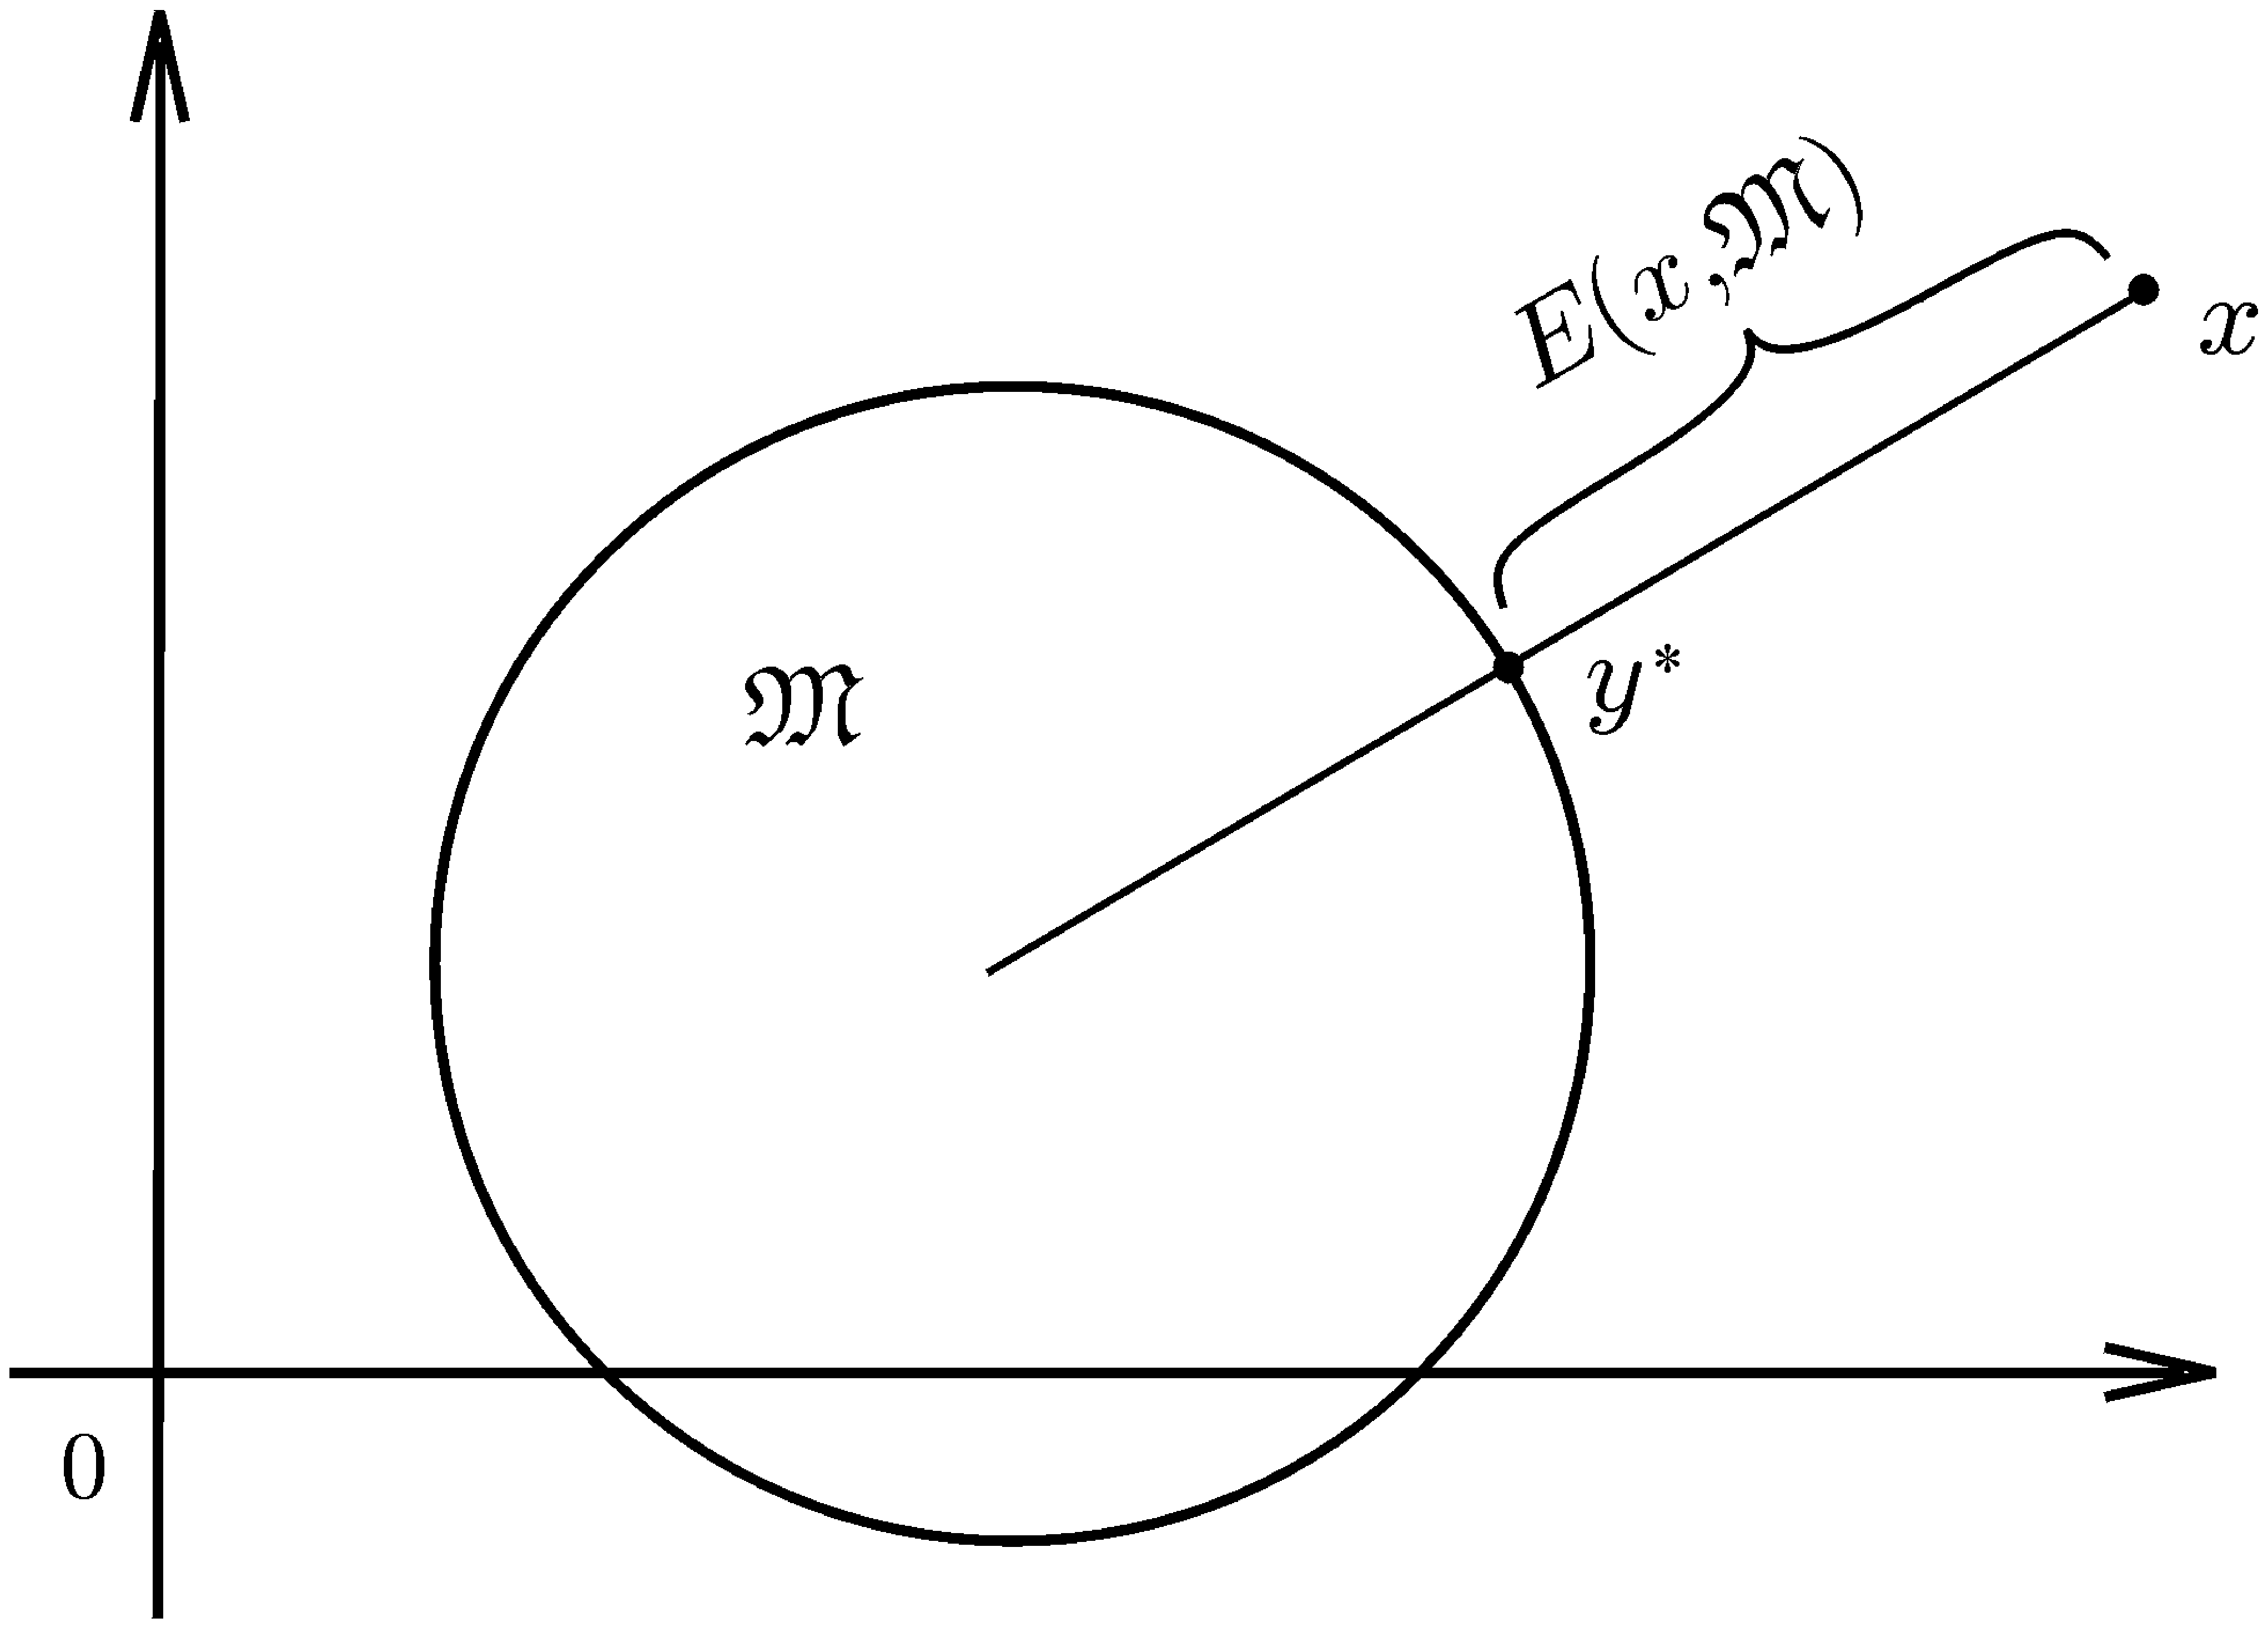
\includegraphics[width=0.5\textwidth]{pict01-1.eps}
\end{center}
 \bigskip
 \refstepcounter{ris}\label{r1-1}

 \centerline{Рис.~\theris}
 \bigskip
\end{figure}

% \bigskip
% \begin{picture}(70,170)
% \put(70,160){\special{em: graph pict1-1.eps}}
% \end{picture}
%\hbox to 0.5cm {}{\special{em:graph pict1.pcx}}
%\vspace{6cm}
% \bigskip
% \refstepcounter{ris}\label{r1-1}

% \centerline{Рис.~\theris}
% \bigskip

%%%%%%%%%%%%%%%%%%%%%%%%%%%%%%%%%%%%%%%%%%%%%%%%%%%%%%%%%%


Наилучшее приближение и наилучший элемент обладают и другими
неприятными особенностями. Поясним на
примере.

\begin{Example}
$X=C[a,b],$~ $-\infty < a < b < +\infty$ {(функция $f\in
C[a,b]$,} {если она непрерывна на $[a,b]$)},
{$\|f\|_C=\max\limits_{x\in[a,b]}|f(x)|$,}
$\ro(f,g)=\|f-g\|_C$. В качестве $\G M$ возьмем $\G M=\{c \}$
{--} множество констант $c \in \bR${, точнее, множество}
{постоянных функций}. Тогда, очевидно, {для любой} $ f
\in C[a,b]$ существует единственный наилучший элемент $c^* \in
\G M$, {
$$
c^* = \frac{\max\limits_{x\in[a,b]}{f(x)}+\min\limits_{x\in[a,b]} {f(x)}}{2}
$$
}
(см. рис.~\ref{r1-2}).
\end{Example}

%%%%%%%%%%%%%%%%%%%%%%%%%%%%%%%%%%%%%%%%%%%%%%%%%%%%%%
%\vspace{5mm}

\begin{figure}[ht]
\begin{center}
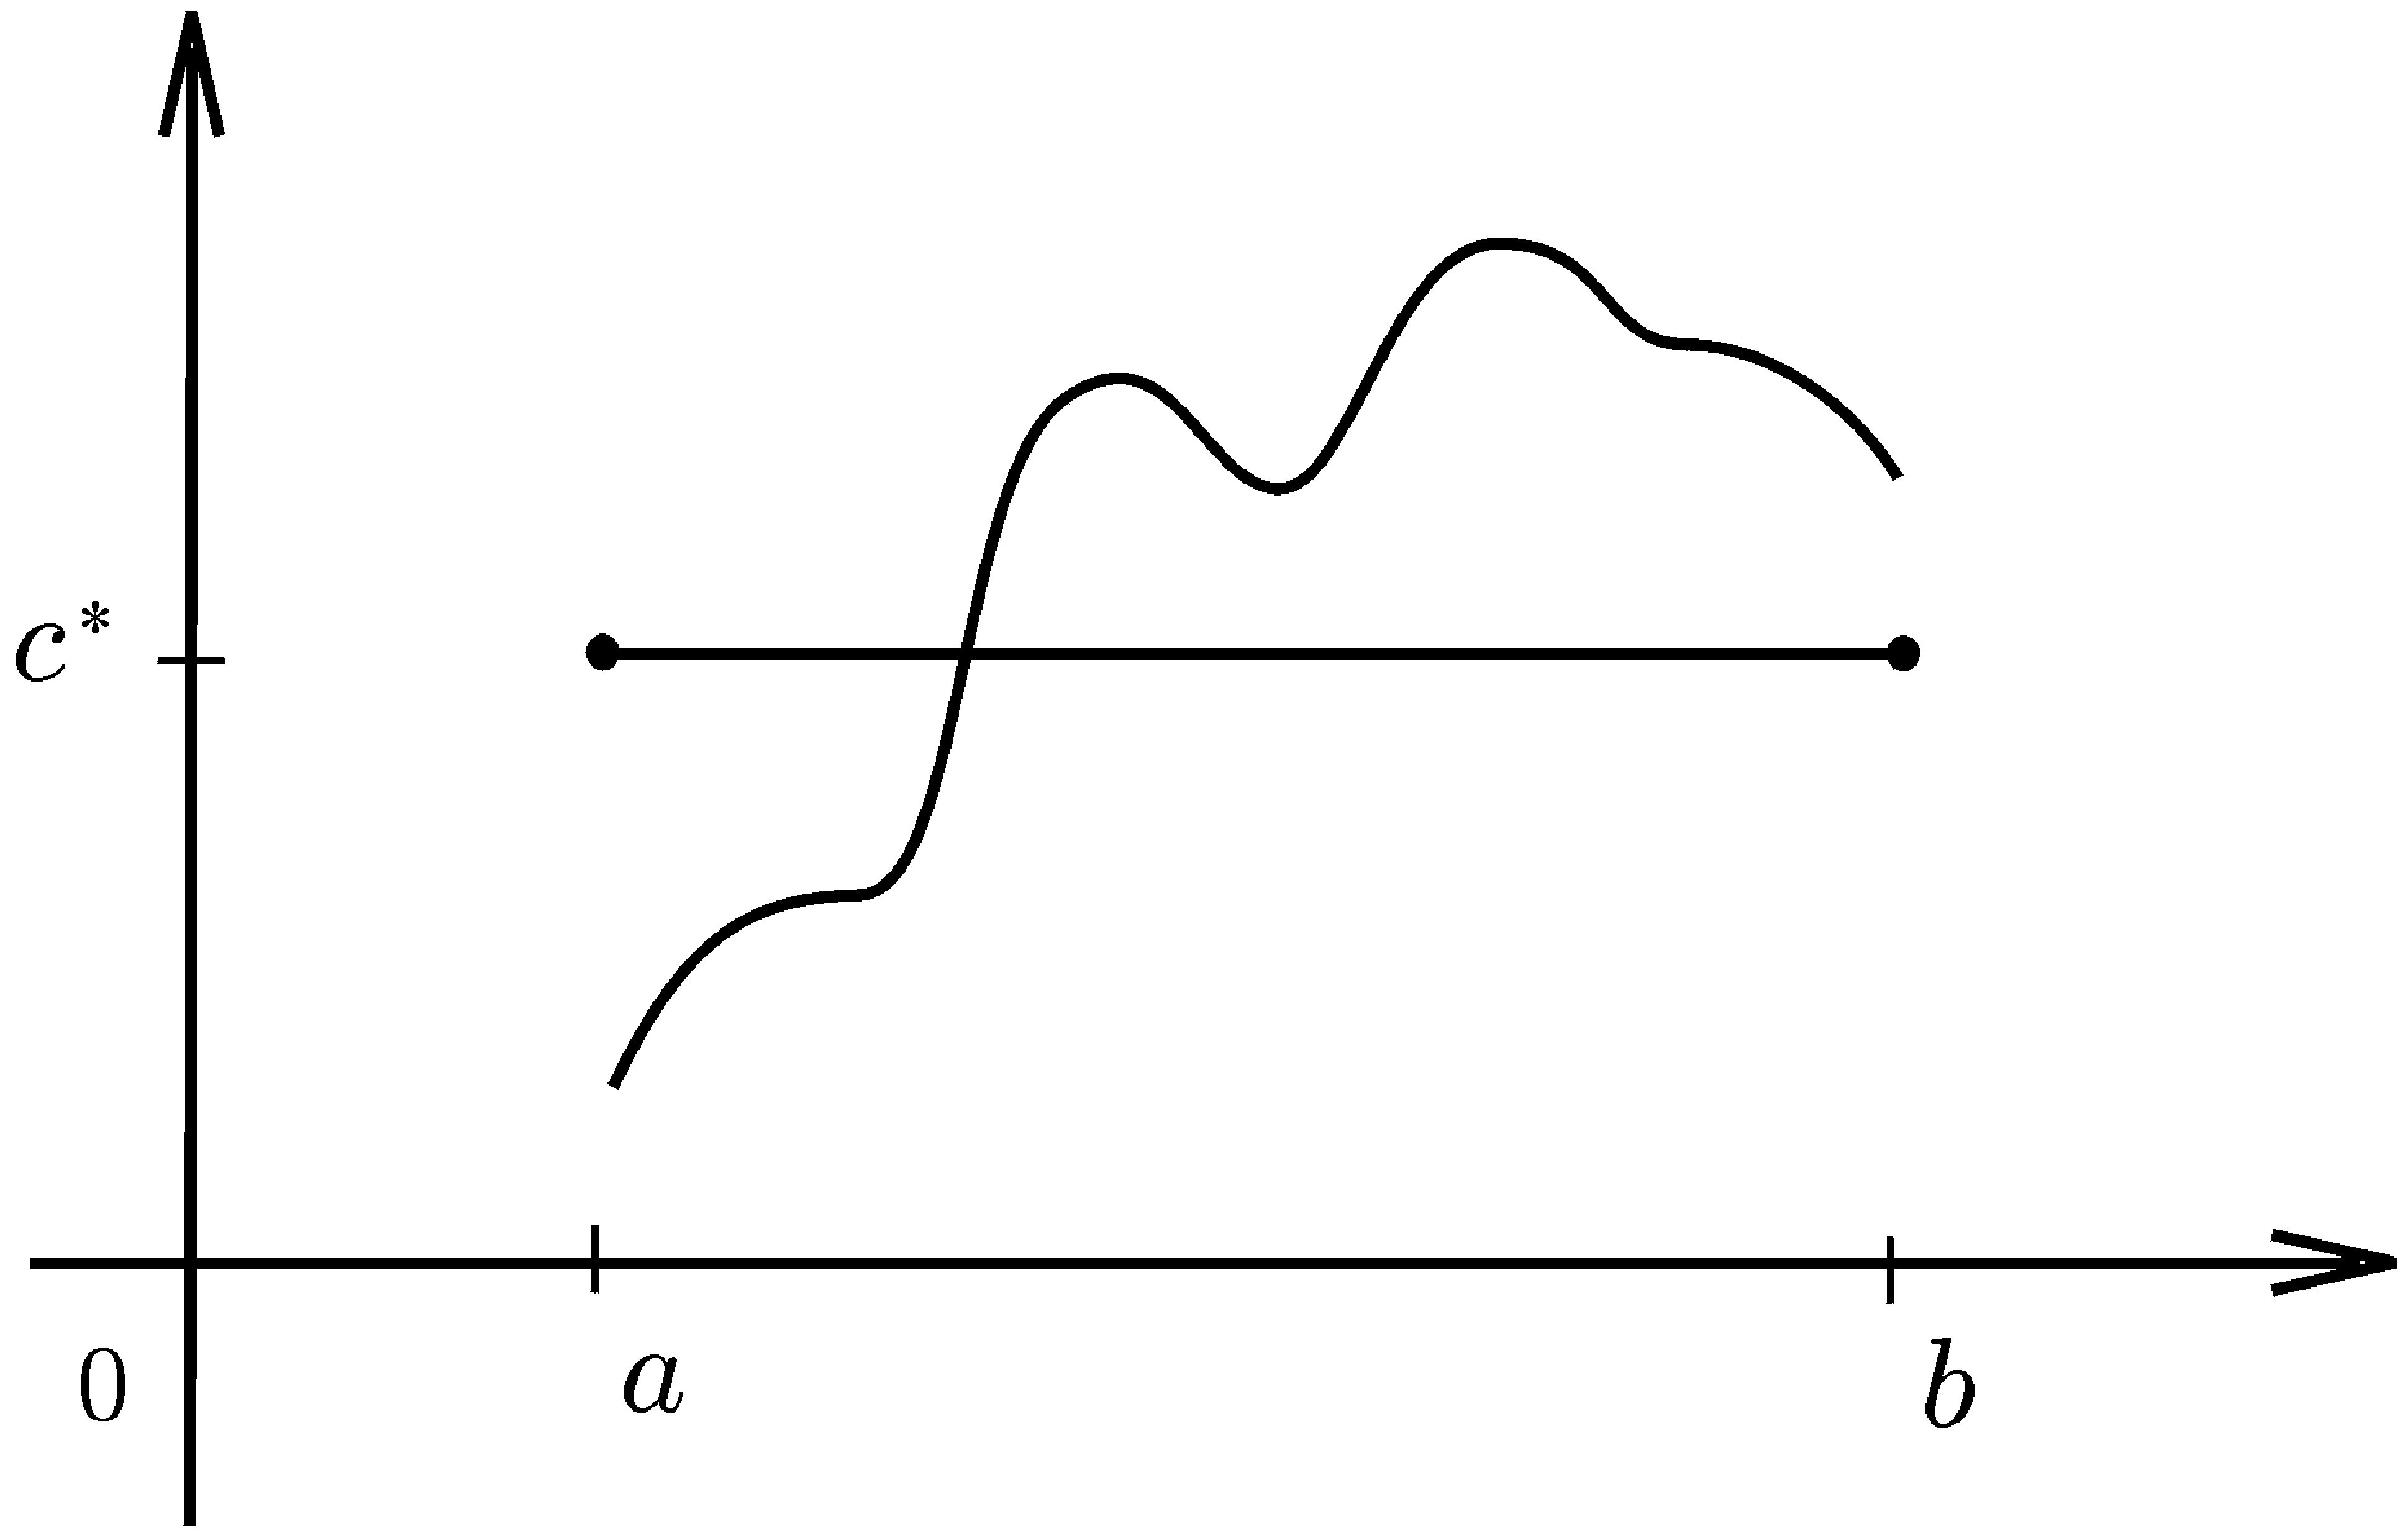
\includegraphics[width=0.5\textwidth]{pict01-2.eps}
\end{center}
 \bigskip
 \refstepcounter{ris}\label{r1-2}

 \centerline{Рис.~\theris}
 \bigskip
\end{figure}

% \bigskip
% \begin{picture}(70,170)
% \put(100,160){\special{em: graph pict01-2.eps}}
% \end{picture}
% \refstepcounter{ris}\label{r1-2}

% \centerline{Рис.~\theris}
% \bigskip

%%%%%%%%%%%%%%%%%%%%%%%%%%%%%%%%%%%%%%%%%%%%%%%%%%%%%%%%%%



Итак, возникает оператор {наилучшего приближения} $A${,}
любой функции $f \in C[a,b]$ ставящий в соответствие
наилучший элемент $c^* \in \G M$: $A(f)=c^*(f).$ Этот оператор не является линейным.
Действительно, если мы возьмем $f_1$ и $f_2$ как на рис.~\ref{r1-3}, то
$c^*(f_1)=c^*(f_2)=c^*(f_1+f_2)=h/2,$ т.\,е. $A(f_1+f_2)\ne A(f_1)+A(f_2).$

%%%%%%%%%%%%%%%%%%%%%%%%%%%%%%%%%%%%%%%%%%%%%%%%%%%%%%
%\vspace{5mm}

\begin{figure}[ht]
\begin{center}
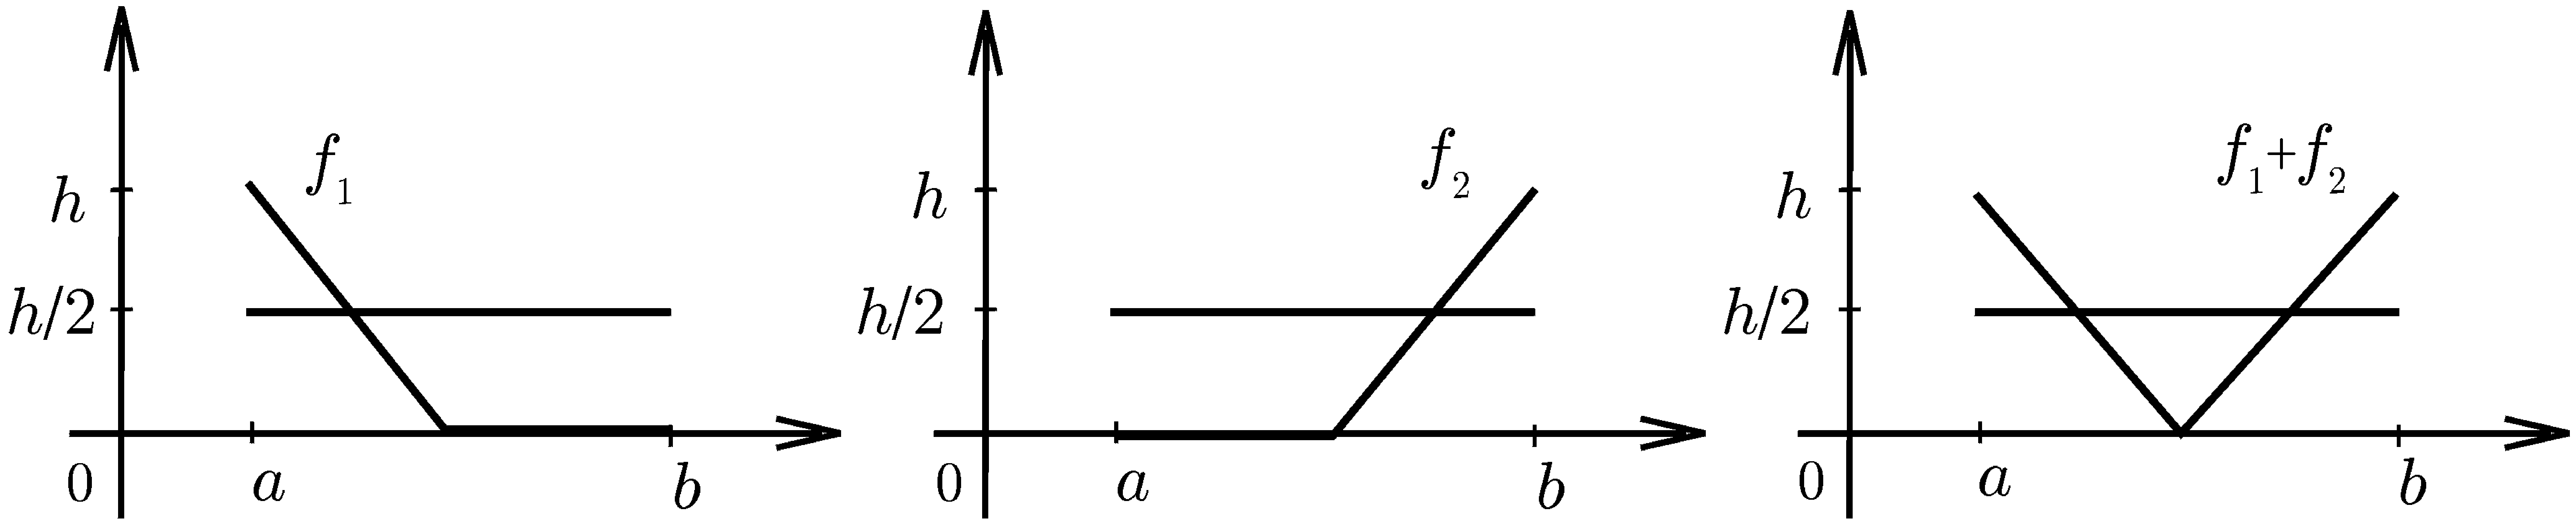
\includegraphics[width=0.9\textwidth]{pict01-3.eps}
\end{center}
 \bigskip
 \refstepcounter{ris}\label{r1-3}

 \centerline{Рис.~\theris}
 \bigskip
\end{figure}



% \bigskip
% \begin{picture}(0,120)
% \put(-10,120){\special{em: graph pict01-3.pcx}}
% \end{picture}
%\centerline{рис. 3} \vspace{5mm}
% \refstepcounter{ris}\label{r1-3}

% \centerline{Рис.~\theris}
% \bigskip

Итак, в некоторых функциональных пространствах {оператор наилучшего} {приближения}
$A$ не является линейным, значит,
{найти} $E{(x)}$ и $y^*{(x)}$ {может} {оказаться трудной задачей. Поэтому рассматривают и
более простые методы} {приближения. В частности, различные линейные методы.}

\section{Линейная задача теории приближения}

Пусть $X=C[a,b]=C$ и $\Cal L$ -- некоторое {подпространство} из $C$ и пусть $A$~--
линейный оператор из $C$ в $C$ и {$Af \in \Cal L$} для любой функции $f \in C[a,b].$
Будем говорить в этом случае, что в $C$ задан линейный метод $A$ приближения элементов
{из} $C$ посредством подпространства $\Cal L$. {Для $f$ в качестве приближающего
выступает элемент $Af$.}

Интерполирование -- первый классический метод линейного приближения.

\section{Лагранжево интерполирование}

Пусть функция $f \in C[a,b]$ (пока можно считать, что значения $f(x) \in \bC$~--
множеству комплексных чисел).

Возьмем на $[a,b]$ {различные точки} $x_k\ (k=0,1,\ldots,n)$. Можно считать, что
$a \le x_0 <x_1< \cdots <x_n \le b.$ Точки $\{x_k\}$ будут называться {\it узлами
интерполяции}.

Задача состоит в том, чтобы для узлов $\{x_k\}$ и для любого набора {чисел} $\{y_k\}\
(k=0,1,\dots ,n)$ построить многочлен $p_n \in \mathcal{P}_n,$
\[
  p_n(x)=a_0+a_1x+\cdots +a_n x^n,
\]
такой, что $p_n(x_k)=y_k$\  $(k=0,1,\dots ,n).$

Возникают вопросы:
\smallskip
1) Всегда ли задача разрешима?
\smallskip
2) Сколько имеется решений?
\smallskip

Здесь для определения коэффициентов $a_i\ (i=0,1,\dots,n)$ получается система линейных
уравнений с определителем Вандермонда, не равным $0.$ Следовательно, для любых $x_k$ и
любых $y_k$ имеется единственное решение. Поэтому достаточно {выписать} решение в
явном виде. {С этой целью для} любого $k=0,1,\dots,n$ построим фундаментальный
многочлен {$l_k(x)$} лагранжевой интерполяции, соответствующий $k$-му узлу, -- это
многочлен степени $n$, обладающий свойствами: $l_k(x_i)=\delta_{i,k}$, где
$\delta_{i,k}$ -- символ Кронекера, $\delta_{k,k}=1, \ \delta_{i,k}=0$ при $i \ne k$.

Очевидно,
\[
  l_k(x)=\frac{(x-x_0)(x-x_1)\cdots (x-x_{k-1})(x-x_{k+1})\cdots (x-x_n)}
         {(x_k-x_0)(x_k-x_1)\cdots (x_k-x_{k-1})(x_k-x_{k+1})\cdots (x_k-x_n)}.
\]
Обозначим $\omega(x)=\prod_{k=0}^n(x-x_k).$
Тогда
$$
\omega'(x_k)=
      (x_k-x_0)(x_k-x_1)\cdots (x_k-x_{k-1})(x_k-x_{k+1})\cdots (x_k-x_n)
$$
и, следовательно,
\[
 l_k(x)=\frac{\omega(x)}{(x-x_k)\omega'(x_k)}.
\]
Ясно, что
\[
 p_n(x)=p_{n}(x,\{y_k\},\{x_k\})=
 %\sum_{k=0}^n y_k
 %\frac{\omega(x)}{(x-x_k)\omega'(x_k)}=
 \sum\limits_{k=0}^n y_k l_k(x)
\]
-- искомый многочлен. Интерполяционный многочлен
рассматриваемой задачи, записанный в этой форме, называется {\it
интерполяционным многочленом Лагранжа}.

Пусть теперь $f \in C[a,b],$~ $\{x_k\}$~-- узлы интерполяции, а $y_k=f(x_k)$\
$(k=0,1,\dots ,n).$ Тогда для любой функции $f \in C[a,b]$ и любых узлов
{интерполяции} $\{x_k\}$\  $(k=0,1,\dots ,n)$ существует единственный многочлен
$$
p_n(x,f)=p_n(x,f,\{x_k\})=\sum\limits_{k=0}^n f(x_k) l_k(x)
$$
степени не выше $n$, который удовлетворяет условиям
\[
 p_n(x_k,f)=f(x_k)\qquad (k=0,1,\dots ,n).
\]
Таким образом, возникает {оператор} $P_n:\ f \longmapsto p_n(x,f)$ {из} $C{[a,
b]}$ в $C{[a,b]}$. {Отметим} простейшие свойства {этого оператора.}

1) {Если} $f \in \Cal P_n$, то для любых узлов $\{x_k\}$
имеем $p_n(x,f)\equiv f(x),$ т.\,е. $P_{n}(f)=f.$

2) $f \to P_n(\cdot,f)$
~-- линейный (т.\,е. однородный, аддитивный) ограниченный оператор:
$$
  P_n(c_1f_1+c_2f_2) \equiv c_1P_n(f_1)+c_2P_n(f_2),\qquad
  f_i\in C[a,b],\qquad c_i\in \bR\qquad (i=1,2),
$$
и для любой функции
$f\in C[a,b]$
$$
  \|p_n(\cdot,f)\|_C \le L_n\|f\|_C,\ \ \mbox{где}\ \
  L_n=\|P_n\|_C^C<\infty.
$$

Более того,
$$
|p_n(x,f)| \le L_n(x)\|f\|_C.
$$
Здесь $L_n(x)=\sum{|l_k(x)|},$~ $L_n =
\|L_n(x)\|_C$. Оба неравенства вытекают из формулы для $p_n(x, f) = p_n(x,f,\{x_k\})$. В
пространстве $C[a,b]$ они являются точными.

{Действительно, определим
при фиксированном $\xi \in [a,b]$ функцию $f_\xi(x)$ так,
чтобы она удовлетворяла условиям}

{а) $f_\xi(x)=\sign{l_k(\xi)}$ при $x=x_k\  ( k=0,1,\ldots,n)$,}

{б) $|f_\xi(x)| \le 1$ при $x \in [a,b]$,}

{в) $f_\xi(x)$ непрерывна по $x$ на $[a,b]$.}

{Тогда будем иметь
$$
\|f_\xi\|_C=1,
\qquad  p_n(x, f_\xi) = \sum\limits^n_{k=0}{f_\xi(x_k)l_k(x)}
$$
и, в частности,
$$
  p_n(\xi, f_\xi) = \sum\limits^n_{k=0}{|l_k(\xi)|} =
  L_n(\xi)\|f_\xi\|_C,
$$
а выбирая здесь в качестве $\xi$ точку $x^*$ максимума на $[a,b]$ функции $L_n(x)$,
получим
$$
  p_n(x^*,f_{x^*}(\cdot)) = L_n\|f_{x^*}\|_C
$$
и, следовательно,
$$
  \|p_n(x,f_{x^*}(\cdot))\|_C = L_n\|f_{x^*}\|_C.
$$}

{Таким образом, константа $L_n$ есть норма оператора $P_n\colon f \longmapsto p_n(x,f):$
$$
  \|P_n\|_{C \to C} = L_n.
$$
А для любого фиксированного $x \in [a,b]$ величина $L_n(x)$ является нормой функционала
$P_x(f)=p_n(x,f)$ в $C[a,b]$:
$$
\|P_x(f)\| = L_n(x),
$$
так как
$$
|P_x(f)| \le L_n(x)\|f\|_C\qquad \forall\ f \in C[a,b]
$$
и
$$
|P_x(f_x(\cdot))|=L_n(x)\|f_x\|_C.
$$}

{Константа $L_n$ называется \textit{константой Лебега}, а $L_n(x)$ --
\textit{функцией Лебега} линейного метода $p_n(x, f, \{x_k\})$ приближения функций $f$ из
$C[a,b]$ интерполяционными многочленами Лагранжа. Ясно, как эти понятия распространяются
на другие линейные методы приближения.}

{Метод интерполирования тем <<лучше>>, чем меньше его норма, т.\,е. константа Лебега. При
$n$ фиксированном $L_n$ зависит от узлов интерполирования $\{x_k\}$. Если $[a,b]=[-1,1]$,
то можно узлы выбрать так, что $L_n=\dfrac{2}{\pi}\ln{n} + O(1)$~ $(n \to +\infty)$, а
именно, в качестве узлов интерполяции нужно взять нули многочлена Чебышева
$$
T_{n+1}(x)=\cos({(n+1)}\arccos{x}).
$$}

3) Тождества Коши.

Из свойства 1) и формулы для интерполяционного многочлена {при $f(x)\equiv 1$}
получаем {тождество}
\[ \sum\limits_{k=0}^n l_k(x) \equiv 1, \]
{а при} $f(x)=(x-u)^j$~ $(j=1,\dots ,n;\ u\in \mathbb C)$ {-- тождества}
$$
(x-u)^j\equiv \sum\limits_{k=0}^n (x_k-u)^j l_k(x) \qquad (j=1,2,\ldots,n),
$$
{откуда при} $u=x$ следует, {что}
\begin{equation}\label{f1-1}
\sum\limits_{k=0}^n (x_k-x)^j l_k(x)\equiv 0\qquad (j=1,\ldots ,n).
\end{equation}
Эти тождества при $\{x_n\}\subset [a,b]$ справедливы для
всех $x\in \mathbb C.$

\section{Оценка погрешности интерполяционной \\ формулы
Лагранжа. Неравенства Лебега}

Пусть $\{x_k\}_{k=0}^n$~-- узлы интерполяции, $f \in C[a,b],$ $p_n(x,f)$ --
соответствующий интерполяционный многочлен Лагранжа. Можно написать
\[
  f(x)=p_n(x,f)+R_n(x,f),
\]
где $R_n(x,f)$~-- остаточный член. Очевидно, в узлах интерполяции $R_n(x_k,f)=0$~
$(k=0,\dots ,n).$ Требуется оценить $R_n(x,f)$ для любого фиксированного $x \in [a,b],$
а также оценить $\|R_n(\cdot ,f)\|_{C[a,b]}.$

Оказывается, для оценок остаточного члена лагранжевой интерполяции {достаточно} знать
$L_n(x),$ $L_n$ {и} $E(f ,\Cal P_n)_C=\inf\limits_{q \in \Cal P_n}\|f-q\|_{{C}}.$
Именно, имеют место неравенства Лебега
\[  |R_n(x,f)|\le (L_n(x)+1)E(f ,\Cal P_n)_C,             \]
\[  \|R_n(\cdot ,f)\|_{{C}} \le (L_n+1)E(f ,\Cal P_n)_C.             \]
Для доказательства воспользуемся тем, что $P_n(x,f)$~-- линейный оператор, и
$P_n(x,q)=q(x)$ для любого $q \in \Cal P_n$ ({аналогичные неравенства} Лебега
{возникают} и {для} более {общих линейных методов, сохраняющих элементы $\Cal
P_n$ на месте}). Имеем
\begin{multline*}
  |R_n(x,f)|=|f(x)-p_n(x,f)|=|f(x)-q(x)-p_n(x,f-q)|\le  \\
  \le |f(x)-q(x)|+L_n(x)\|f-q\| \le
      (L_n(x)+1)\|f-q\|_{{C}}, \qquad q \in \Cal P_n.
\end{multline*}
Значит, если в качестве $q$
возьмем наилучший элемент для $f$
в $\Cal P_n,$
то получим
\[  |R_n(x,f)|\le (L_n(x)+1)E(f ,\Cal P_n)_C,\qquad x\in [a,b],   \]
откуда следует, что
\[  \|R_n(\cdot ,f)\|_{{C}} \le (L_n+1)E(f ,\Cal P_n)_C.             \]

\section{Остаточный член в форме Коши\\
 для интерполяционной формулы Лагранжа}

%%%%%%%%%%%%%%%%%%%%%%%%%%%%%%%%%%%%%%%%%%%%%%%%%%%%%%%%%
{Функция $f \in C^{(n+1)}[a,b],$ если $f$ непрерывна на $[a,b]$ вместе с производными
до} {порядка $n+1$ включительно.}

\begin{teo}\label{t1-1}
Пусть $f \in C^{(n+1)}[a,b].$ Тогда для любого $x \in [a,b]$ существует {точка} $\xi
\in (a,b)$ {такая}, что
\[
  R_n(x,f)=\frac{f^{(n+1)}(\xi)}{(n+1)!}\omega (x)
\]
$(${здесь $\xi=\xi(x,f,\{x_k\})$},~ $n+1$~-- число узлов
интерполяции$).$
\end{teo}

\begin{proof}
{Доказываемая формула, очевидно, верна для $x=x_k$}
{$(k=0,\dots ,n)$} ($\xi$ может любой точкой). Зафиксируем {$x \in [a,b],$~ $x \ne x_k,$}
и рассмотрим вспомогательную функцию
\[
  F(t)=f(t)-p_n(t)-K\omega (t),
\]
где {$p_n(t)=p_n(t,f,\{x_k\}),$~ $K=R_n(x,f)/ \omega (x), \ \omega(x) \ne 0.$} Заметим,
что $F(t)$ при $t=x_k$ равна нулю $(k=0,\dots ,n)$ и $F(x)=0$ по выбору $K.$ Следовательно, функция
{$F(t)$} имеет нули в ${n+2}$ различных точках. Применим обобщенную теорему Ролля, из
которой следует, что найдется точка $\xi \in (a,b)$ такая, что $F^{(n+1)}(\xi)=0$.
{Но} $F^{(n+1)}(\xi)=f^{(n+1)}(\xi)-K\cdot (n+1)!,$ значит,
$K=f^{(n+1)}(\xi)/(n+1)!,$ откуда {для} $R_n(x,f)=K\omega(x)$ {получаем}
\[
  R_n(x,f)=\frac{f^{(n+1)}(\xi)}{(n+1)!}\omega (x)
\]
и теорема доказана.
\end{proof}

\begin{Remark}[геометрическое]
{Остаточный} член не обязан менять знак в узлах {интерполяции вслед за
$\omega(x).$} Графики $f(x)$ и $p_n(x,f)$ могут соприкасаться, как показано на
рис.~\ref{r1-4}.
\end{Remark}

%%%%%%%%%%%%%%%%%%%%%%%%%%%%%%%%%%%%%%%%%%%%%%%%%%%%%%
%\vspace{5mm}

\begin{figure}[ht]
\begin{center}
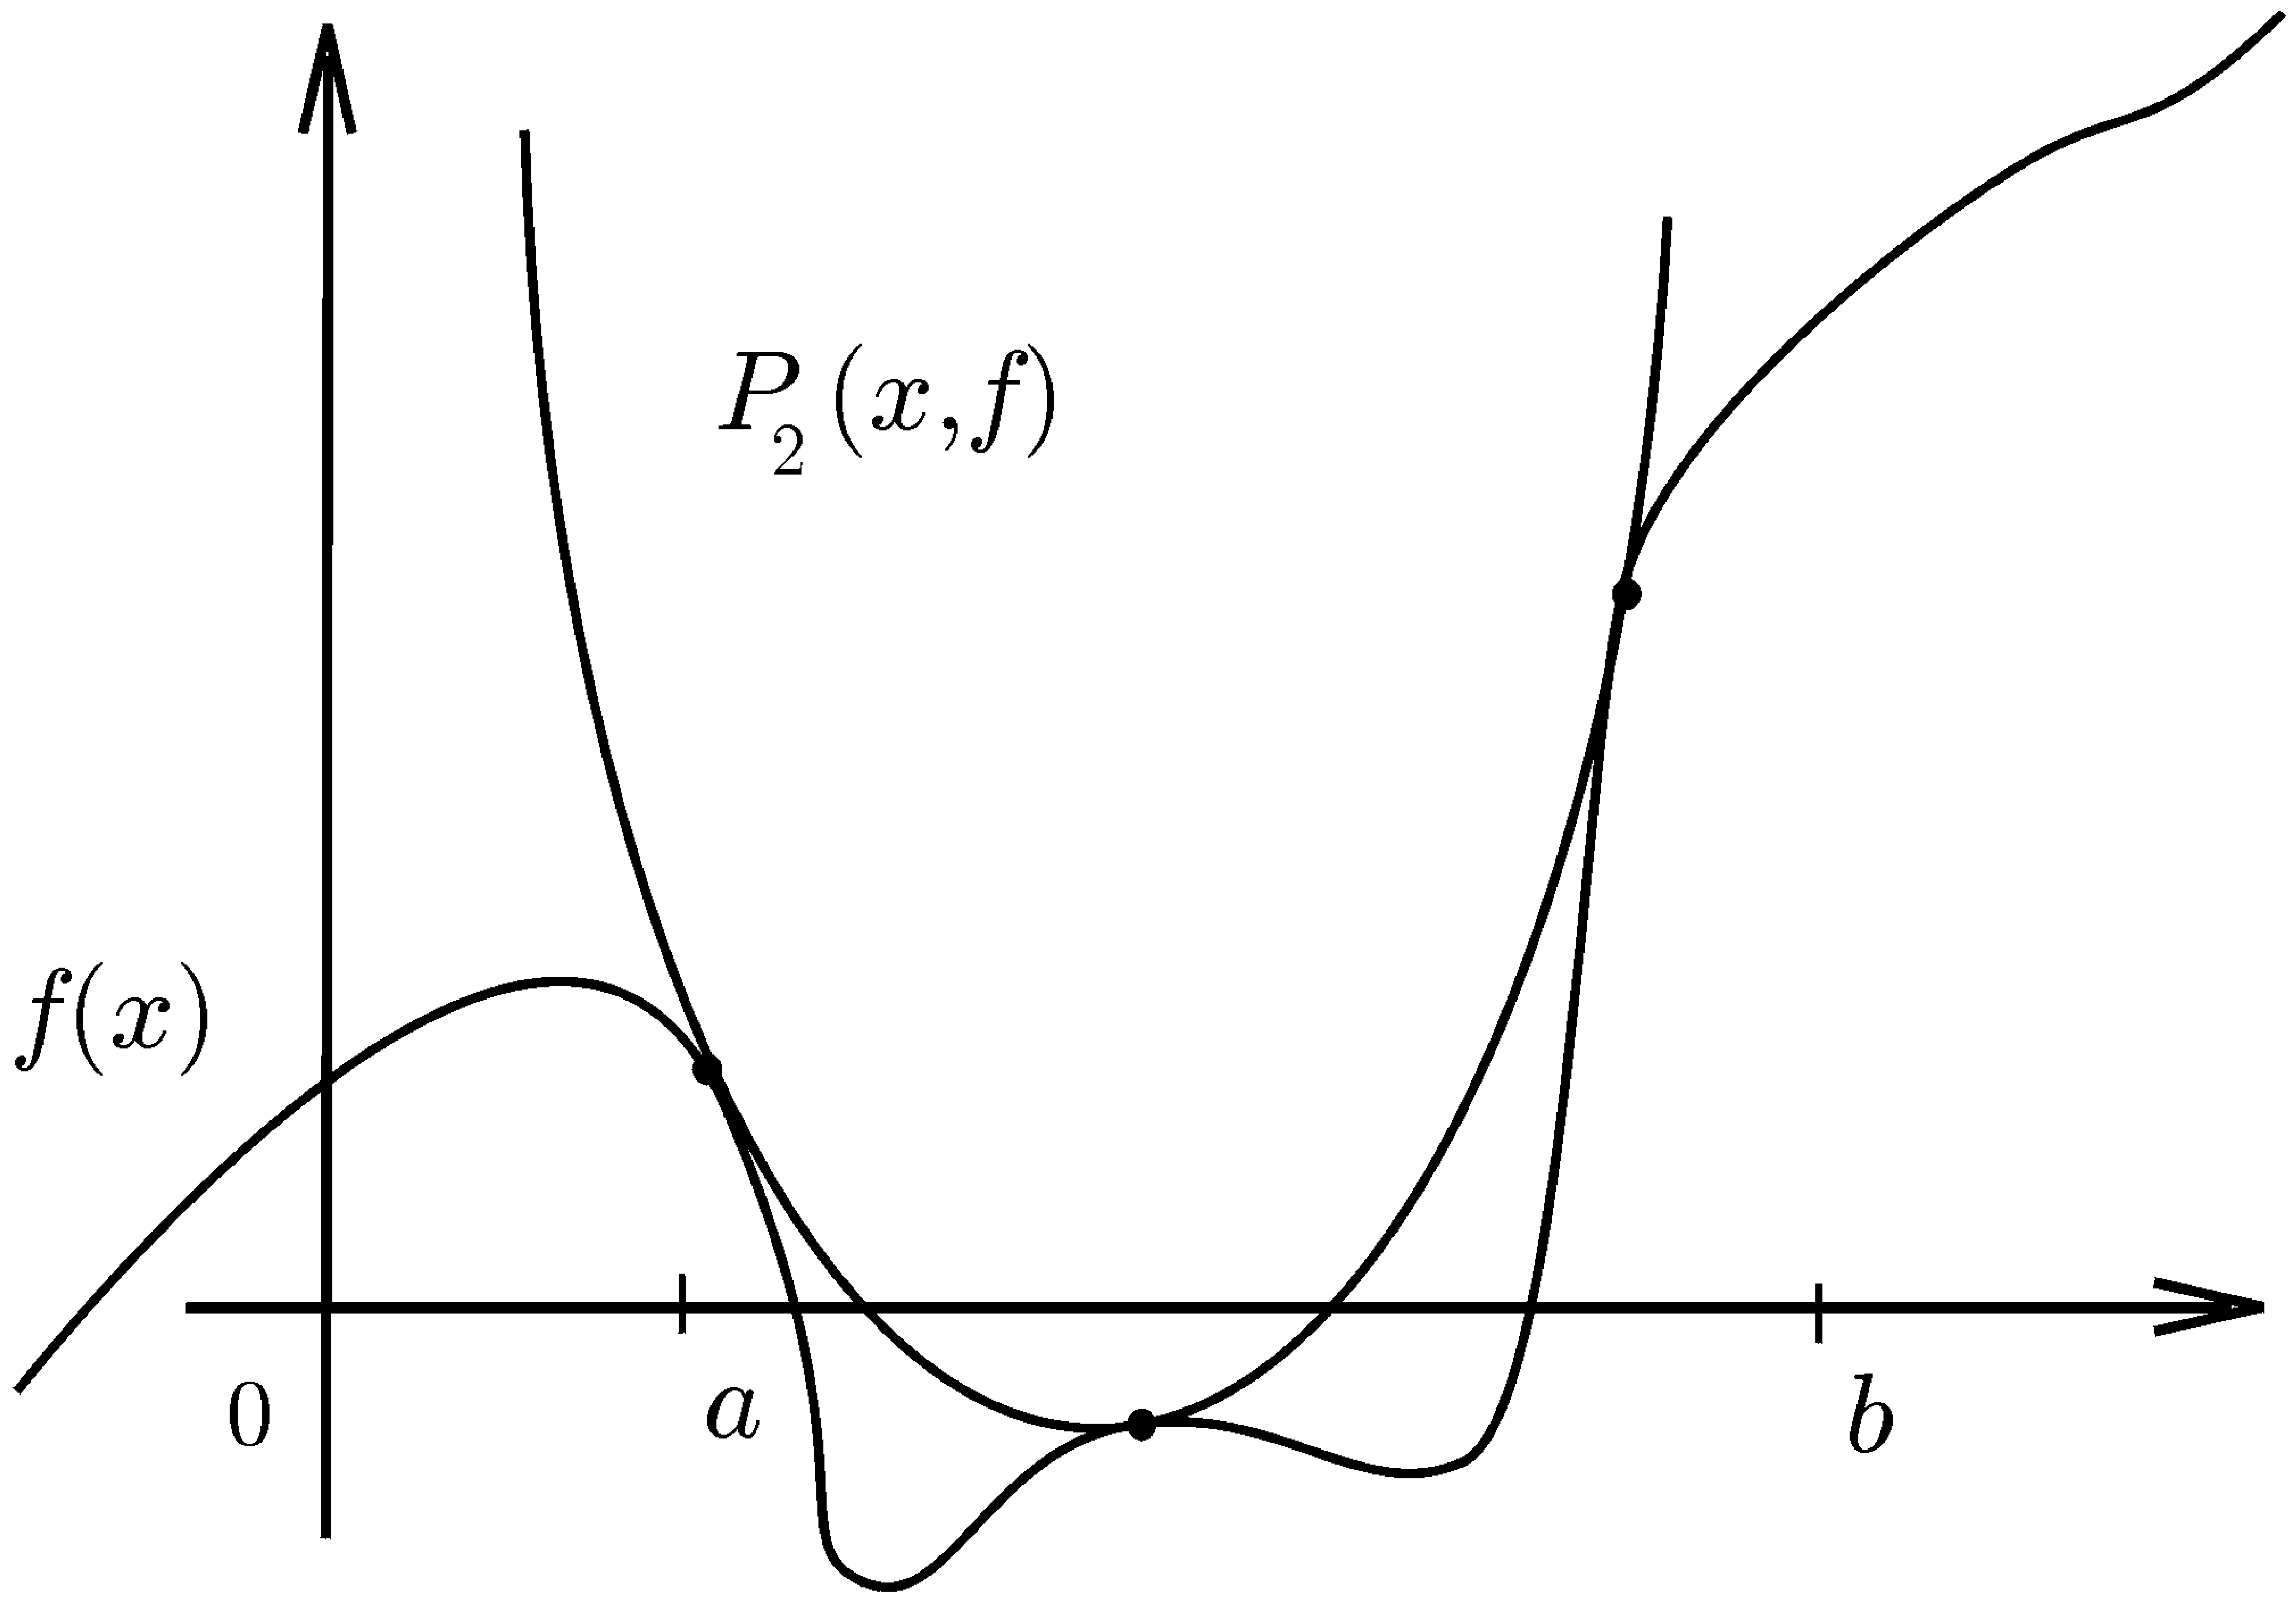
\includegraphics[width=0.5\textwidth]{pict01-4.eps}
\end{center}
 \bigskip
 \refstepcounter{ris}\label{r1-4}

 \centerline{Рис.~\theris}
 \bigskip
\end{figure}



% \bigskip
% \begin{picture}(70,190)
% \put(90,190){\special{em: graph pict01-4.pcx}}
% \end{picture}
%\hbox to 0.5cm {}{\special{em:graph pict4.pcx}}
%\vspace{6cm}

% \refstepcounter{ris}\label{r1-4}

% \centerline{Рис.~\theris}
% \bigskip

%%%%%%%%%%%%%%%%%%%%%%%%%%%%%%%%%%%%%%%%%%%%%%%%%%%%%%%%%%
%\noindent \hskip3.0cm {\rm рис. 4}
%\bigskip



Но есть достаточное условие того, что остаточный член меняет знак в узлах. Как видно из
формулы для остаточного члена интерполяции в форме Коши, {\it если} $f^{(n+1)}(x)$
{\it сохраняет знак}, {\it то} $R_n(x,f)$ {\it меняет знак в узлах интерполяции и только в них}.

Обозначим $M_{n+1}(f)=\max\limits_{x \in [a,b]}f^{(n+1)}(x).$

\begin{Corollary}
\[
 \|R_n(\cdot ,f) \|_C \le \frac{M_{n+1}(f)}{(n+1)!}\|\omega(\cdot ) \|_C .
\]
\end{Corollary}

\begin{task}
При каком выборе узлов интерполяции величина $\|\omega(\cdot ) \|_C$
наименьшая?
\end{task}

 Оказывается {это будет,} когда $\omega$~-- многочлен
Чебышева\footnote{{Свойства} многочлена Чебышева приводятся в лекции 2.}
{$\widetilde{T}_{n+1}(x,I)$ $(I=[a,b]).$}
{Действительно, } $\omega(x)=x^{n+1} +a_{n}x^n+ \dots +a_0.$ Так {что}
\[
  \inf \|\omega(\cdot)\|_{C[a,b]}=\|\widetilde{T}_{n+1}(\cdot{, I})\|_{C[a,b]},
\]
где $\widetilde{T}_{n+1}{(\cdot, I)}$~-- многочлен Чебышева
на $[a,b],$ т.\,е. наименее
уклоняющийся на $[a,b]$ от нуля многочлен {степени $n+1$} со
старшим коэффициентом 1. В частности, $\widetilde{T}_{n+1}(x,[-1,1])=
\dfrac1{2^n}\cos(n+1)\arccos x.$


\section{Теорема Хаара об интерполяции в $\mathbb R^N$}

Мы рассматривали {задачу} интерполяции на {$D=[a,b] \subset
\bR^1$} т.\,е. в одномерном случае. Пусть теперь множество {$D \subset \bR^N,\ N\ge 2.$}

{{В о п р о с ы}. \hspace{1em}}

Имеет ли смысл задача {интерполяции} в многомерном случае?

Существуют ли действительные функции {$f_0(x),f_1(x),\dots,f_n(x),$~ $x \in
\overline{D} \subset \bR^N,$} ({\it интерполяционные системы на} $D$), {линейными
комбинациями которых} можно интерполировать {любой набор чисел $\{y_k\}_{k=0}^n$ в} любых
{несовпадающих узлах} $\{x_k\}_{k=0}^n \in D?$

Легко убедиться, что интерполяционные системы, состоящие из
разрывных функций, существуют на любом множестве мощности континуум. Для
этого достаточно рассмотреть взаимно однозначное
отображение отрезка на множество и взять порожденные им функции,
соответствующие рассмотренной нами на отрезке
интерполяционной системе $1,x,x^2,\dots ,x^n.$

Далее будет показано, что задача интерполяции многочленами разрешима
в комплексной области. А ответ на вопрос об $\bR^N$ дает следующая теорема.

\begin{teo}[А.\,Хаар]
Если $N>1$ и множество $D\subset \mathbb R^N$ имеет
внутренние точки, т.\,е. {$\inter {D} \ne \varnothing,$} и если $n \ne 0,$ то {в
$D$ не существует} непрерывных действительных интерполяционных систем {$($т.\,е.
систем, которыми можно интерполировать} при любом выборе узлов $\{x_k\}^{n}_{k=0}$
любой набор чисел $\{ y_k\}_{k=0}^n).$
\end{teo}

\begin{proof}
Возьмем внутреннюю точку и ее некоторую
окрестность $\Delta \subset D,$
и пусть {$\{x_k\}_{k=0}^n \subset \Delta.$}

%%%%%%%%%%%%%%%%%%%%%%%%%%%%%%%%%%%%%%%%%%%%%%%%%%%%%%

\begin{figure}[ht]
\begin{center}
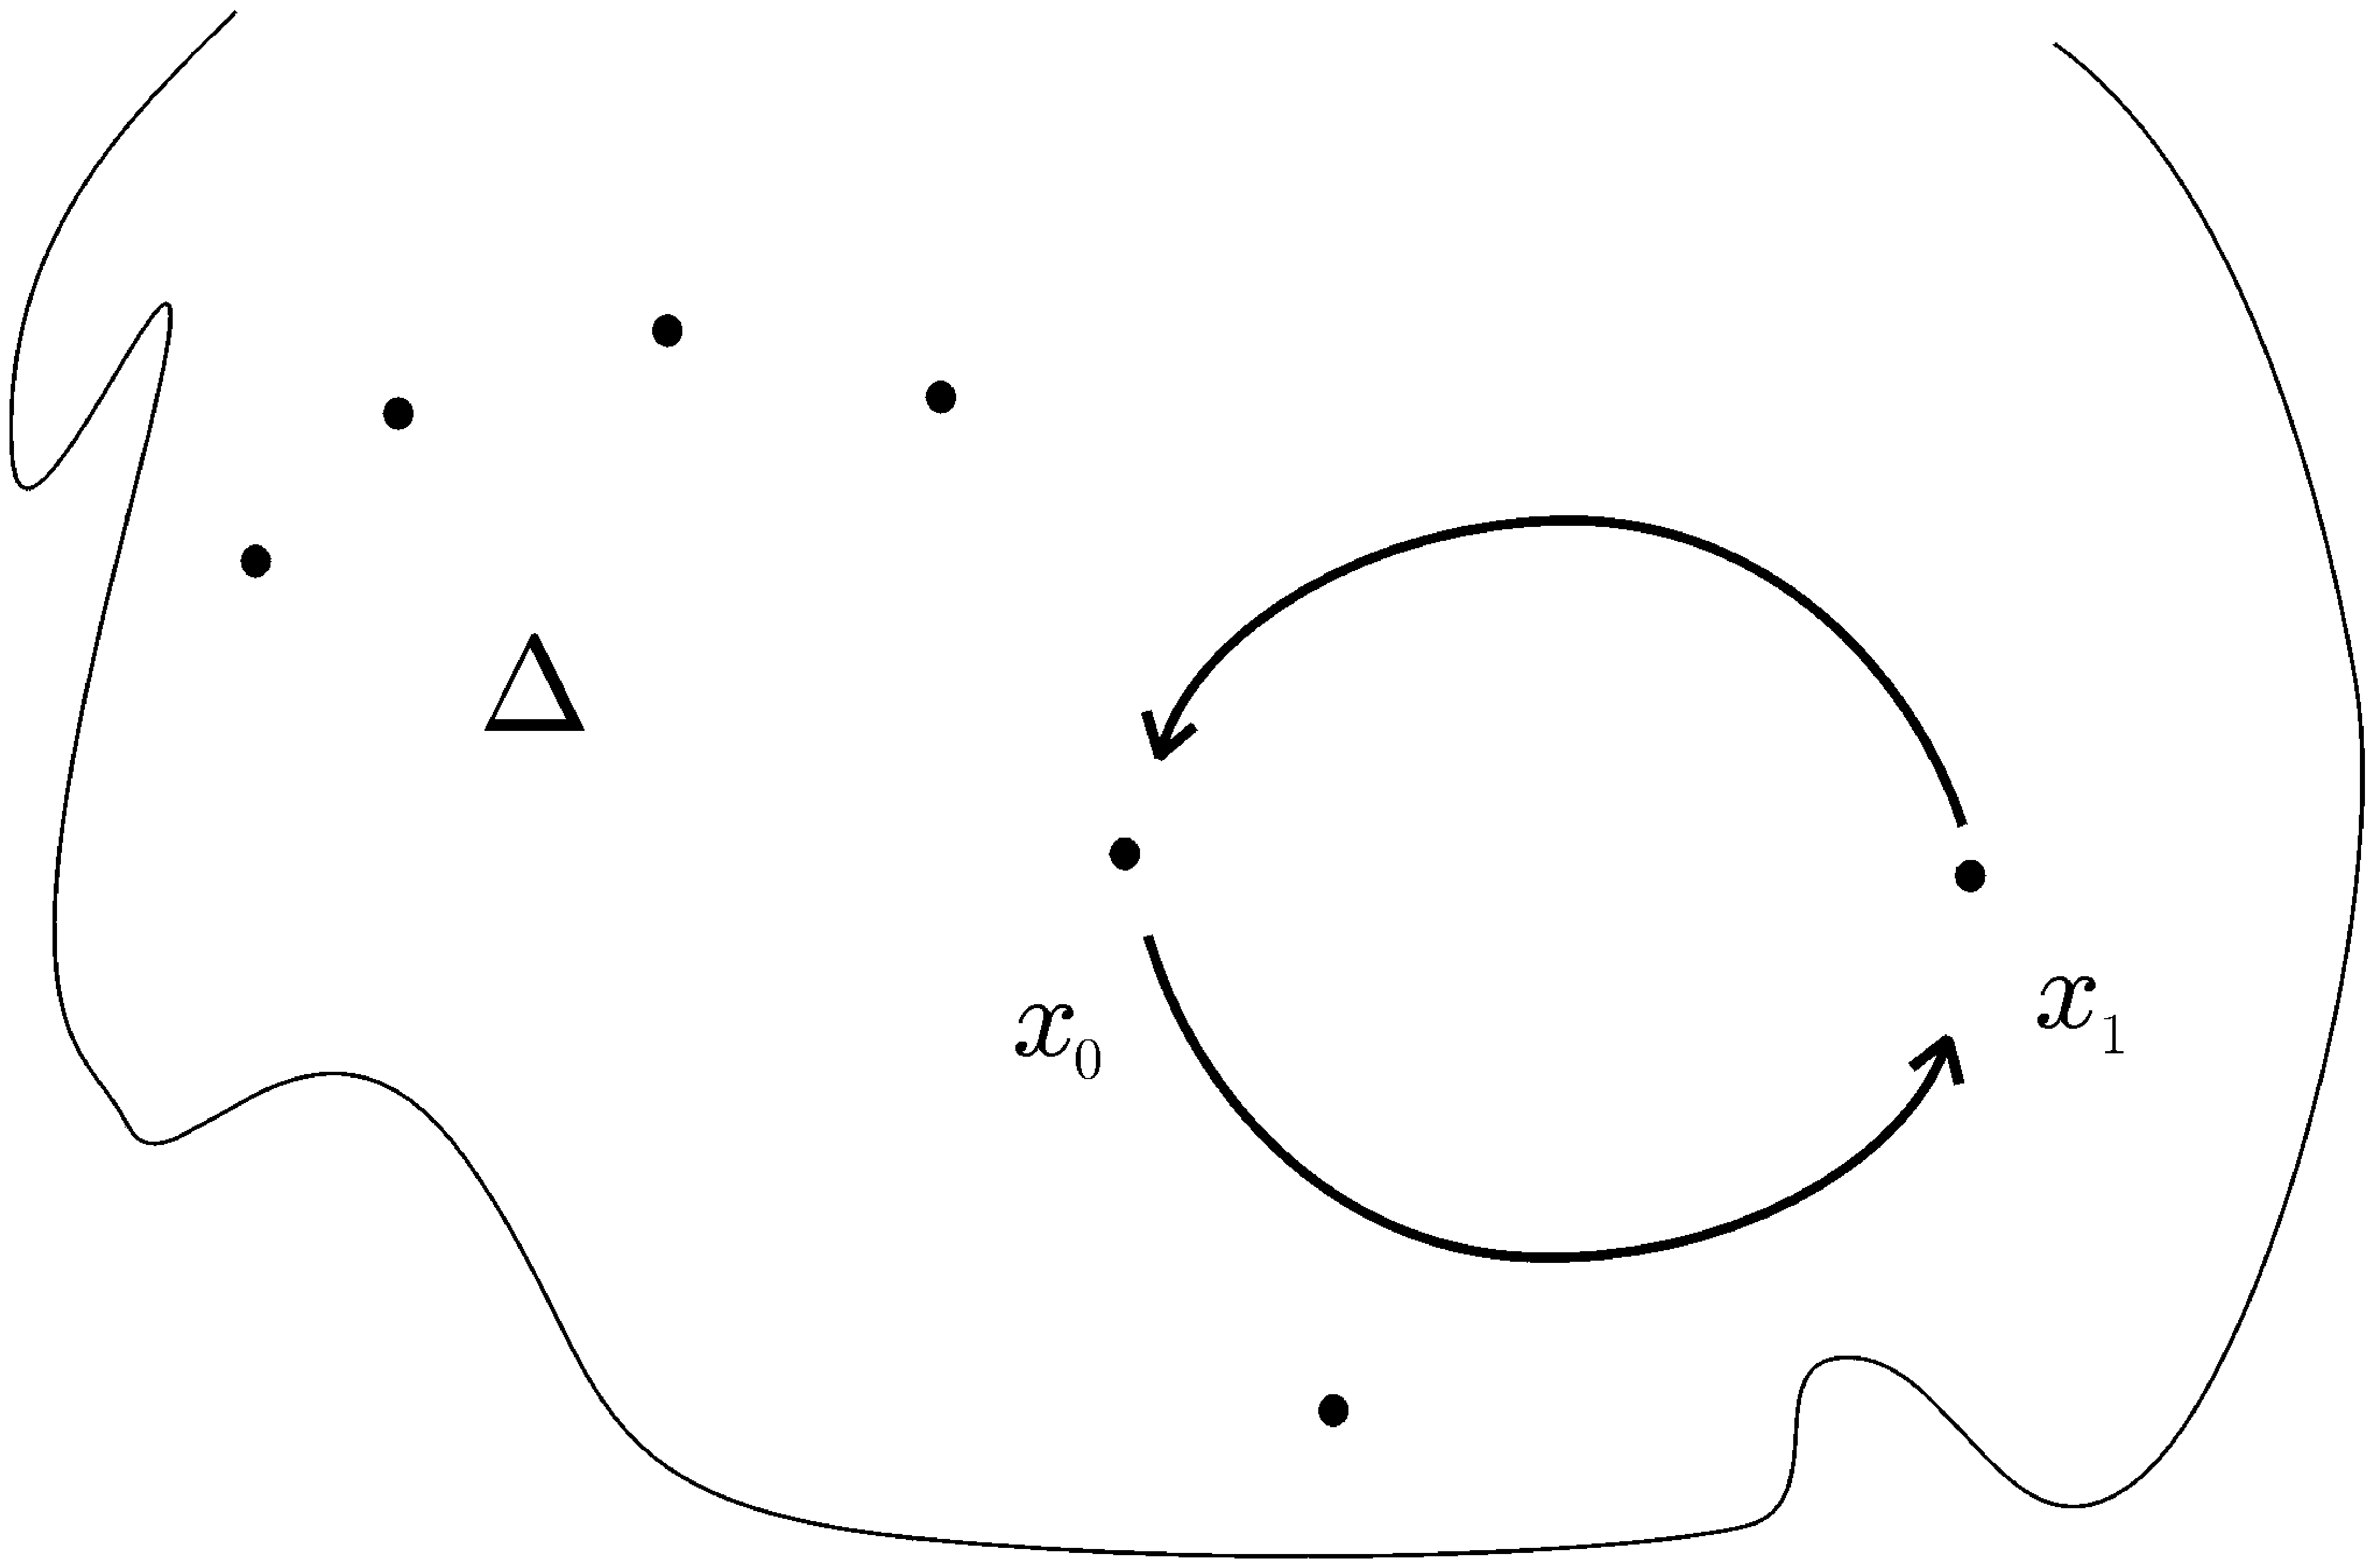
\includegraphics[width=0.5\textwidth]{pict01-5.eps}
\end{center}
 \bigskip
 \refstepcounter{ris}\label{r1-5}

 \centerline{Рис.~\theris}
 \bigskip
\end{figure}




\noindent Если система {$\{f_k\}$~ $(k=0,\ldots,n)$} интерполяционная, то система
уравнений
\[
  \sum\limits^{n}_{k=0}c_k f_k(x_i)=y_i\qquad ({i}=0,\dots ,n),
\]
разрешима для любых {наборов чисел $\{y_k\}$}. {Отсюда следует, что} $\det
(f_k(x_i)) \ne 0$ {для любых $\{x_k\} \subset \Delta$.} По условию функции
$f_k$ непрерывны, следовательно, определитель непрерывен как функция от точек
$\{x_i\}$ в области $\Delta.$ Теперь все точки $x_k$ в $\Delta,$ кроме двух, например
$x_0$ и $x_1$, оставим на месте, а $x_0$ и $x_1$ будем непрерывно переводить друг в
друга {(см. рис.~\ref{r1-5})} {так, что при движении все $n+1$ точки
остаются различными и принадлежат $\Delta$.} Определитель будет непрерывно меняться,
{оставаясь вещественным,} и переменит знак (поменяются местами две строки
определителя). Следовательно, { при каком-то} {промежуточном наборе точек он
обращался в нуль. Это противоречие доказывает } {теорему. }
\end{proof}

\begin{Remark}
Непрерывные действительные интерполяционные
системы не существуют не только на множествах с непустой
внутренностью, но даже на континууме
с точкой ветвления.
\end{Remark}
Действительно, поменяем точки $x_0$ и $x_1$ {местами, перемещая их непрерывно,} как
показано на рис.~\ref{r1-6}, знак определителя изменится, следовательно, он обращался в
нуль, чего  не {должно} быть для непрерывных интерполяционных систем.

%%%%%%%%%%%%%%%%%%%%%%%%%%%%%%%%%%%%%%%%%%%%%%%%%%%%%%
 \bigskip
\begin{figure}[h]
\begin{center}
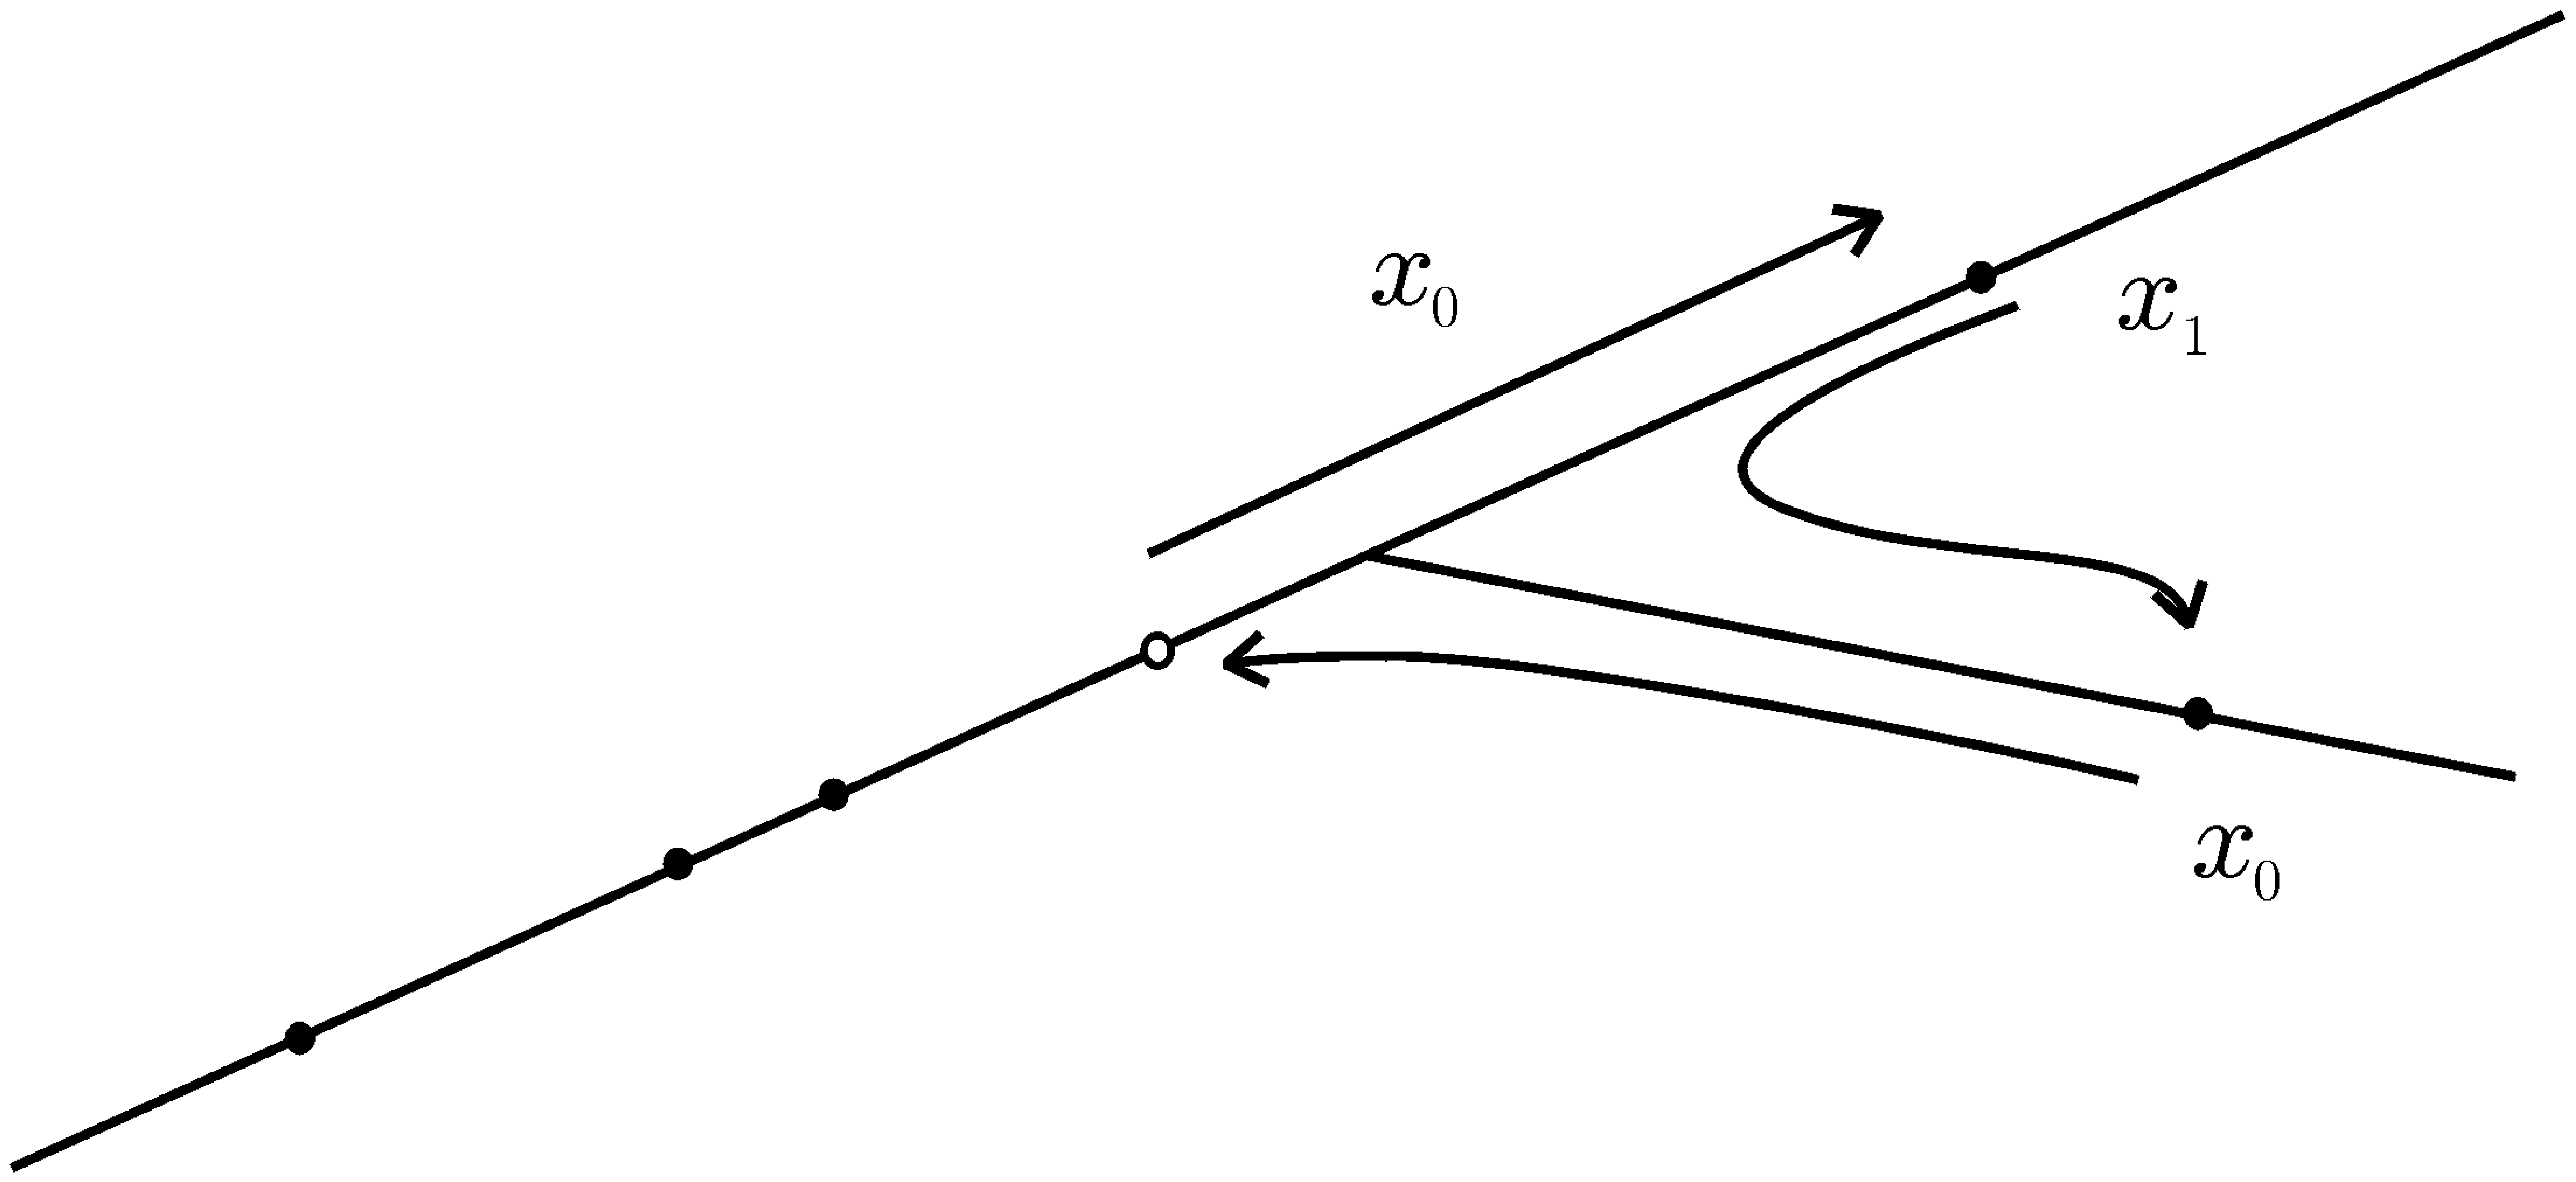
\includegraphics[width=0.5\textwidth]{pict01-6.eps}
\end{center}
 \bigskip
 \refstepcounter{ris}\label{r1-6}

 \centerline{Рис.~\theris}
 \bigskip
\end{figure}


%%%%%%%%%%%%%%%%%%%%%%%%%%%%%%%%%%%%%%%%%%%%%%%%%%%%%%%%%%
%\noindent \hskip3.0cm {рис. 6}
%\bigskip

\noindent
Так что классическая задача интерполяции ограничена
рассмотрением ее на отрезке.

\begin{task}
При чем здесь отрезок? Пусть {$f_k(x) \in \bR^m$}\  $\forall\ x \in K \subset
\bR^M$\ {$(k=0,1,\ldots,n).$} На каких множествах $K$ существуют
непрерывные интерполяционные системы, а для каких не существуют?
\end{task}

При $m \ge 2$ окончательного ответа на эти вопросы нет. Известно (теорема
Мерхьюбера), что при $m=1$ и $n \ge 1$ компактное множество $K$ должно быть гомеоморфно
части
{окружности или всей окружности.
В последнем случае $n$ должно быть четным, т.\,е.} {число базисных функций -- нечетным.
}

 % Лекции Сергея Борисовича Стечкина
% Внесены исправления Ю.Н.Субботина и Н.И.Черныха, версия 30.06.2009
% Внесены исправления Н.И.Черныха, версия 29.07.2009
% Внесена грамматическая и ТеХ-правка М.Дейкаловой, версия 05.08.09

\chapter{Оценка остаточного члена интерполяции.\\
Многочлены Чебышева} %%{Лекция 2.}

\section{Оценка остаточного члена}

Пусть {$\{x_k\}^n_{k=0}$}~-- узлы интерполяции на $[a,b]$ и функция $f$ имеет непрерывную
${n+1}$ производную на $[a,b],$\ {$p_n(x,f)$~--
соответствующий} интерполяционный многочлен {Лагранжа} для $f,$\ $R_n(x,f)=f(x)-p_n(x,f)$~--
остаточный член интерполяции. Мы получили оценку
для $\|f(\cdot)-p_n(\cdot ,f)\|_C$ через наилучшее приближение
$E_n(f, \Cal P_n)_C$ (см. неравенство Лебега) и, значит, {(}так как $E_n(f,
\Cal P_n)_C \le \|f\|_C${)} через $\|f\|_C.$ Получили также оценку
$\|R_n(\cdot ,f) \|_C$ через максимум $f^{(n+1)}$ на отрезке, т.\,е. через
$\|f^{(n+1)}\|_C$ (см. {следствие из теоремы~\ref{t1-1})}. Следовательно, имеем оценки
\[
  \|f(\cdot )-p_n(\cdot ,f)\|_C \le
               \begin{cases}
                   \Cal K_0 \|f\|_C ,\\
                   \Cal K_{n+1} \|f^{(n+1)}\|_C ,
               \end{cases}
\]
где $\Cal K_0$ и $\Cal K_{n+1}$ -- соответствующие
независящие от функции константы. Попробуем оценить $\|R_n(\cdot ,f)\|_C$ через
{$\|f^{(m+1)}\|_C,$} т.\,е. получить оценки
\begin{equation}\label{lab1}
  \|R_n(\cdot ,f) \|_C \le  \Cal K_{m+1} \|f^{{(m+1)}}\|_C
\end{equation}
и для других $m,$ где $K_{m+1}=K_{m+1}(n)$ не зависят от $f.$
Если такие оценки справедливы, то, взяв функцию $f\in {\cal P}_m$,
у которой {$\|f^{(m+1)}(\cdot )\|_C=0$} получим, что $\|R_n(\cdot ,f)
\|_C=0,$ т.\,е. $f(x) \equiv p_n(x ,f)$ {~--} многочлен степени не выше
$n.$ Так что получаем {необходимое} ограничение на {числа $m,$}
для которых могут быть верны эти оценки: {$m \le n.$} Оценить $\|R_n(\cdot ,f) \|_C$
через нормы производных более высокого порядка нельзя,
так как из условия $f^{(m+1)}(x) \equiv 0,$~ $m > n,$ не следует, вообще
говоря, что $f(x) \equiv p_n(x ,f)$ (например, если $f$ есть
многочлен порядка {$m>n$}).

\begin{lemma}
Условие $m \le n$ является и достаточным условием для справедливости
оценки~$(\ref{lab1}).$
%$\|R_n(\cdot ,f) \|_C$
%через {$\|f^{(m+1)}(\cdot )\|_C.$}
\end{lemma}

\begin{proof}
Интерполяционная формула Лагранжа для $f$ имеет вид
\[
  p_n(x,f)=\sum\limits_{k=0}^n f(x_k) l_k(x).
\]
Используя тождество Коши $\sum\limits_{k=0}^n l_k(x) \equiv 1,$ получаем
$$
R_n(x,f)=f(x)-\sum\limits_{k=0}^nf(x_k)l_k(x)=\sum\limits_{k=0}^n \{f(x)-f(x_k) \} l_k(x).
$$
Запишем для $f(y)$ формулу Тейлора порядка $m$ в точке $x$ с остаточным
членом в интегральной форме
\[
  f(y)=f(x)+p(x,y)+\frac{1}{m!}\int_x^y (y-t)^m f^{(m+1)}(t)dt,
\]
где $f(x)+p(x,y)=q_x(y)$~-- многочлен Тейлора функции $f$ в точке $x.$ В частности,
\[
 f(x_k)=f(x)+q_x(x_k)+\frac{1}{m!}\int_x^{x_k} (x_k-t)^m f^{(m+1)}(t)dt,
\]
где
$$
q_x(x_k) = \sum\limits_{s=1}^m\frac{1}{s!}f^{(s)}(x)(x_k-x)^s
$$
($q_x(x_k)$~-- не многочлен по $x$).

Подставим $f(x_k)$ в выражение для $R_n(x,f),$ при этом учтем, что в
силу третьего тождества Коши \eqref{f1-1} при $m \le n$
$$
\sum\limits_{k=0}^n q_x(x_k)l_k(x)=\sum\limits_{{s=1}}^m{\frac{1}{s!}f^{(s)}(x)
 \sum\limits_{k=0}^n{(x_k-x)^s}l_k(x)}\equiv
0.
$$
{Получим}
\[
{  R_n(x,f)=-\frac{1}{m!} \sum\limits_{k=0}^n l_k(x)
                         \int_x^{x_k} (x_k-t)^m f^{(m+1)}(t)dt=
                         \int_a^b K_{n,m}(x,t,\{x_k\}) f^{(m+1)}(t)dt,}
\]
{Можно проверить, что ядро $K_{n,m}(x,t,\{x_k\})$} этого
выражения при каждом $x$ только при $m=n$ не {меняет знак при $t \in
[a,b]$} и только в этом случае можем,
{применив теорему о среднем,} записать
\[
  R_n(x,f)=f^{(n+1)}(\xi) \cdot A(x)\qquad {(\xi = \xi(x, f, K_{n,n})),}
\]
где $A(x)$ от $f$ не зависит. {Но во} всех {рассматриваемых} случаях {(т.\,е.
при $m \le n$)} получим оценку
\[
  |R_n(x,f)| \le \|f^{(m+1)}(\cdot )\|_C
        \int_a^b |K_{n,m}(x,t,\{x_k\})| dt,\qquad x \in [a,b],
\]
из которой следует требуемое неравенство~(\ref{lab1}).
\end{proof}

\section{Многочлены Чебышева}

Многочленами Чебышева $T_n(x)$ {называются функции}
$$
  T_n(x)=\cos (n\arccos x) \qquad (n=0,1,\dots ),\qquad  x \in [-1,1].
$$
Это, действительно, многочлены: положим $x= \cos \theta$,~ {$\theta \in [0, \pi],$} тогда
%\begin{multline*}
$$
\begin{aligned}
T_n(x) &=\cos (n \arccos x)= \cos n\theta = {\frac{1}{2}(e^{in\theta} +
e^{-in\theta})
=} \\
   &=\frac{1}{2}\{(\cos \theta +i \sin \theta)^n+(\cos \theta -i \sin \theta)^n\}.
\end{aligned}
$$
%\end{multline*}
{Следовательно, при $|x| \le 1$}
$$
T_n(x)=\frac{1}{2}\{(x +i \sqrt{1-x^2})^n+(x -i \sqrt{1-x^2})^n\}.
$$
Из последнего выражения видно, что мнимые части {здесь} уничтожаются, {а в}
{вещественной части радикалы отсутствуют}.

\begin{ex}
{Как многочлен, функция $T_n(x)$ определена при всех $x$. Найти} {для него
представление при $|x| > 1$, аналогичное последней формуле.}
\end{ex}

\section{Основные свойства многочленов Чебышева \\
(выражаемые равенствами)}

\vspace{-2mm}
{\bf 1. Рекуррентная формула}
\vspace{3mm}

При $n=0$ и $n=1$ имеем $T_0(x) \equiv 1,$ $T_1(x) \equiv x.$ Из тригонометрического тождества
\[
  \cos (n+1)\theta =2 \cos \theta \cos n \theta -\cos (n-1)\theta
  \qquad (x = \cos{\theta})
\]
следует {рекуррентная формула}
\[
  T_{n+1}(x)=2x T_n(x)-T_{n-1}(x) \qquad (n=1,2,\dots ).
\]
{Имеем также}
$$
 {T_n'(x)=n \sin ({n} \arccos{x})\cdot \frac{1}{\sqrt{1-x^2}} = \frac{n\sin
 n\theta}{\sin{\theta}}.}
$$

Из рекуррентной формулы следует, что коэффициент при старшей степени многочлена
{$T_n(x)$ при $n \ge 1$} равен $2^{n-1}$, так что
\[
  T_n(x)=\cos (n \arccos x) =2^{n-1} x^n+\cdots .
\]
Все нули этого многочлена $x_k=\cos \dfrac{2k-1}{2n}\pi$
$(k=1,2,\dots ,n)$ лежат в~$(-1,1).$ {Точками} экстремумов
на $[-1,1]$ являются {точки} $\widetilde x_k=\cos \dfrac{k
\pi}{n}$ {$(k=0,1,\dots ,n),$} $T_n(\widetilde x_k)=(-1)^k,$
причем при {$k\ne 0$} и {$k \ne n$} выполнено {условие
$T_n'(\widetilde x_k) = 0,$ а $T_n'(1)=n^2,$}\
{$T_n'(-1)=(-1)^{n-1}n^2$. С ростом $n$ нули и точки
экстремума уплотняются у концов} {отрезка $[-1,1]$} (сравним
рис.~\ref{r2-1} и \ref{r2-2}).

%%%%%%%%%%%%%%%%%%%%%%%%%%%%%%%%%%%%%%%%%%%%%%%%%%%%%%
%\hbox to 0.5cm {}{\special{em:graph pict7.pcx}}
%\vspace{6cm} \vspace{5mm} \noindent
%\begin{picture}(0,170)
% \put(0,160){\special{em: graph pict2-1.pcx}}
% \end{picture}

\begin{center}
\begin{picture}(290,100)
\includegraphics[width=0.95\textwidth]{pict02-1.eps}
\end{picture}
%\bigskip
\centerline{\normalsize Рис.~\theris}

\refstepcounter{ris}\label{r2-1}
\end{center}


%\vspace{-3mm}
{\bf 2. Производящая функция}
\vspace{3mm}

Если дана последовательность $\{A_n\},$ то {ее} производящей функцией называется
такая функция $F,$ коэффициенты Тейлора которой равны $A_n.$

Вычислим {$\sum\limits_{n = 0}^{\infty} \cos (n\theta )\ {t^n}.$}
Это действительная часть степенного ряда
\[
  \sum\limits_{{n=0}}^{\infty}\, \exp{(i n\theta)}\ t^n=\frac{1}{1-t\exp{(i \theta)}}
 { =\frac{1-t\exp(-i\theta)}{1-2{t}\cos{\theta}+t^2},}
\]
так что
\[
  \sum\limits_{{n=0}}^{\infty}\, \cos (n\theta )\ {t^n}=
                      \frac{1-t \cos \theta}{1-2t\cos \theta +t^2}
\]
и если $x=\cos \theta,$ то получаем производящую функцию {$F(t)$} для {последовательности}
многочленов Чебышева:
\[
  \sum\limits_{n=0}^{\infty} T_n(x)\,t^n=\frac{1-tx}{1-2tx+t^2}.
\]
{Заменим здесь $x$ на $-x$. Получим}
$$
{\sum\limits_{n=0}^\infty{T_n(-x)t^n} = \sum\limits_{n=0}^\infty{T_n(x)(-t)^n}}
$$
{и, следовательно, $T_n(-x)=(-1)^nT_n(x)$. Конечно, это
свойство можно вывести и из} {явного представления для
$T_n$.}

\ex Как растут {$|T_n(x)|$} в точках $|x|>1$ {с ростом $n$?}

\noindent {У к а з а н и е.\ \ Воспользоваться представлением}
$$
{T_n(x)=\frac{1}{2}\left \{(x +\sqrt{x^2-1})^n+(x -
\sqrt{x^2-1})^n \right\}, \qquad |x|>1.}
$$

\vspace{3mm}
{\bf 3. Дифференциальное уравнение}
\vspace{3mm}

Дифференциальное уравнение, которому удовлетворяют $T_n$:
\[
  (1-x^2)y''-xy'+n^2y=0\qquad (n=0,1,\dots ).
\]
\ex Проверить.

Будем искать {коэффициенты многочлена}
$$
{ T_n(x)=\sum\limits_{k=0}^n a_kx^{n-k}}
$$
{при $n\ge 2$, зная, что он} удовлетворяет этому уравнению. {Знаем также, что}
$a_0=2^{n-1}$ {и} $a_1=a_3=\cdots =0,$ {так как $T_n(-x)=(-1)^nT_n(x).$} Тогда,
подставив в дифференциальное уравнение, получим рекуррентное соотношение
\[
  a_{2k}=-\frac{(n-2k+2)(n-2k+1)}{4k(n-k)}a_{2k-2}.
\]
Следовательно,
\[
  a_{2k}=\frac{(-1)^k n(n-1)\cdots (n-2k+1)}{4^kk!(n-1)\cdots (n-k)}\,{a_0}=
  (-1^k)
  \frac{n}{n-k}C^k_{n-k}2^{n-2k-1}
\]
{и}
$$
  T_n(x)=\sum\limits_{k=0}^{[n/2]} a_{2k}x^{n-2k}.
$$

\begin{Remark}
Несмотря на то, что многочлены Чебышева ограничены единицей на $[-1,1],$ его
коэффициенты при больших $n$ очень большие.
\end{Remark}

\vspace{3mm}
{\bf 4. Ортогональность}
\vspace{3mm}

{Справедливы равенства}
\[
{\frac{2}{\pi}} \int_{-1}^1 \frac{T_n(x)T_m(x)}{\sqrt{1-x^2}}dx={\delta_{n,m}}.
\]

\begin{ex}
{Проверить, сделав замену $x=\cos{\theta}$~ $(0 \le \theta \le \pi)$.}
\end{ex}

\section{Экстремальные свойства многочленов Чебышева}

%\vspace{3mm}
{\bf 1. Первое экстремальное свойство}
\vspace{3mm}

Нормированный многочлен Чебышева $\widetilde T_n(x)=\dfrac{T_n(x)}{2^{n-1}}$ есть многочлен, наименее уклоняющийся от нуля на $[-1,1]$ среди
всех многочленов со старшим коэффициентом $1,$ т.\,е. имеет место {следующее утверждение.}

\begin{teo} \label{teo1extsvo}
Справедливы равенства
%{\it
%\begin{multline*}
$$
\inf_{p \in \Cal P_n,\ p =x^n+\dots} \|p(\cdot )\|_{C[-1,1]} =
            \|\widetilde T_n(\cdot )\|_{C[-1,1]}=\frac{1}{2^{n-1}}=
$$
$$
=\inf_{p \in \Cal P_{n-1}} \|x^n-p(x)\|_{C[-1,1]}= E_{n-1}(x^n)_{C[-1,1]},
$$
%\end{multline*}
где $$\widetilde T(x)=\dfrac{1}{2^{n-1}}T_n(x)=x^n+\dots$$ -- нормированный
многочлен Чебышева. Наилучшее приближение
$E_{n-1}(x^n)_{C[-1,1]}$ достигается на
многочлене $p(x)=x^n-\dfrac{1}{2^{n-1}}T_n(x)\in {\cal P}_n$ {и только на нем}.
\end{teo}

\begin{proof}
Основная идея доказательства заключается в подсчете числа нулей. Пусть есть многочлен
$p \in \Cal P_n$ %с той же нормировкой,
{со старшим коэффициентом, равным $1$,}
но {такой, что}
$$
  \|p(\cdot )\|_{C[-1,1]}  \le \|\widetilde T_n(\cdot )\|_{C[-1,1]}.
$$
Тогда на каждом отрезке, где {$T_n(x)$} изменяется от {$\pm 1$} до {$\mp 1,$ т.\,е. на }
{отрезках $[\widetilde x_k, \widetilde
x_{k+1}]\ (\widetilde x_k=\cos \dfrac{k\pi}{n}$, \
$k={0,1,}\ldots,n$)} разность {$r_{n-1}(x)=\widetilde T_n(x)-p(x)$} обращается в нуль
{(при этом мы учитываем, что если $r_{n-1}=0$ в общем конце двух} {таких отрезков,
то там $T'$ и $p'$ обращаются в нуль и, значит, это
двойной нуль} {разности $r_{n-1}(x)$, см.~рис.~\ref{r2-2}).} {Таким образом,}
степень многочлена $r_{n-1}$ не выше $n-1,$ {а число его
нулей с учетом кратности $\ge n.$} {Следовательно,} $r_{n-1} \equiv 0,$ {$p(x)
\equiv \widetilde T_n(x),$ откуда вытекают все утверждения
теоремы~\ref{teo1extsvo}.} %\pagebreak

%%%%%%%%%%%%%%%%%%%%%%%%%%%%%%%%%%%%%%%%%%%%%%%%%%%%%% %\hbox to 0.5cm {}{\special{em:graph pict8.pcx}} %\vspace{6cm} \vspace{5mm} \noindent
%\begin{picture}(0,210)
% \put(0,190){\special{em: graph pict2-2.pcx}}
% \end{picture}
% \refstepcounter{ris}\label{r2-2}
\begin{center}
\begin{picture}(320,130)
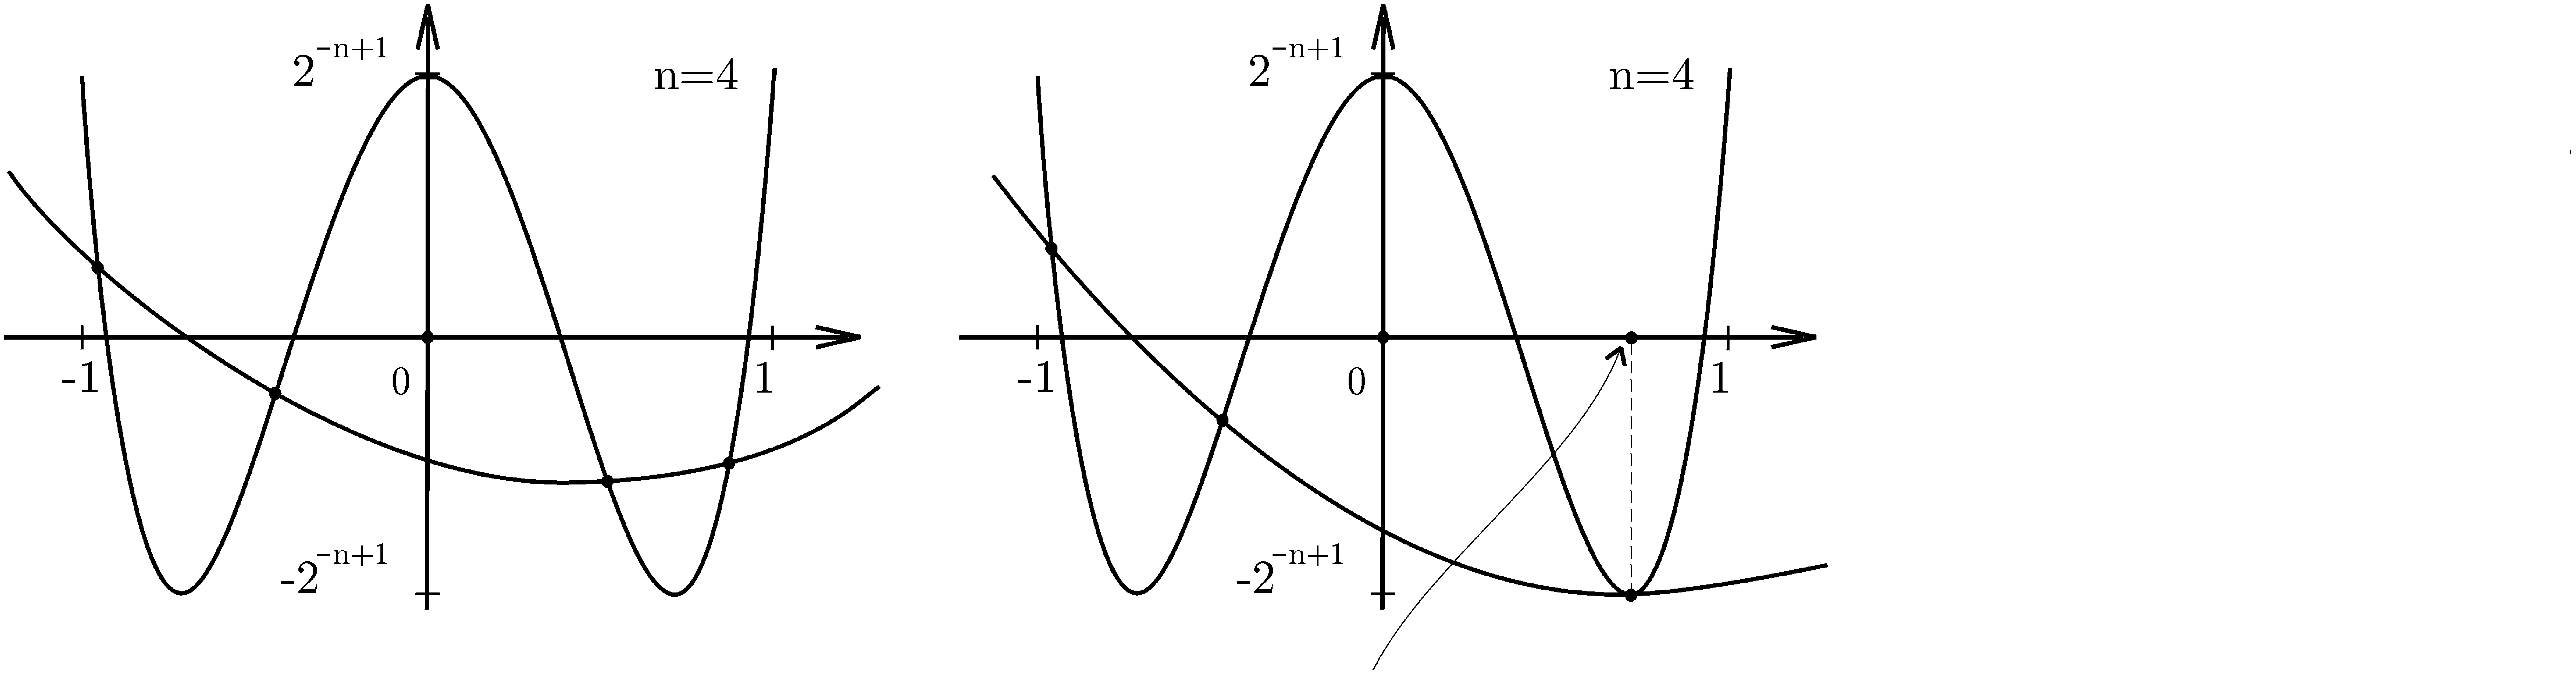
\includegraphics[width=0.99\textwidth]{pict02-2.eps}
\end{picture}
%\bigskip

\refstepcounter{ris}\label{r2-2}
\end{center}

%\centerline{Рис.~\theris}
 \hspace{9.5cm} {Двойной нуль}


 \centerline{\normalsize Рис.~\theris}
\end{proof}

\vspace{2mm}
{\bf 2. Второе экстремальное свойство}
\vspace{3mm}

\begin{lemma}
Пусть {$p \in \Cal P_n,$~ $|p(x)| \not\equiv |T_n(x)|\cdot \|p\|_{C[-1,1]},$} и пусть
$\xi \in \bR,$~ $|\xi |>1.$ Тогда
\[
{ |p(\xi )| < |T_n(\xi)|\cdot \|p(\cdot )\|_{C[-1,1]}.}
\]
{Равенство хотя бы в одной точке $\xi$ вне $[-1,1]$ здесь возможно, только если}
{$p(x)\equiv 0$ {или
$\dfrac{|p(x)|}{\|p\|_{C[-1,1]}}\equiv |T_n(x)|.$}}
\end{lemma}

Д о к а з а т е л ь с т в о\ \ от противного. {Предположим,} {что $\exists\ \xi
\not \in [-1,1]$ :} {$|p(\xi)|
\ge |T_n(\xi)|\cdot\|p\|_{C}$.} Разность
{$q(x)=\dfrac{p(x)}{\|p_n\|_{C[-1,1]}}-T_n(x)$} {-- нетривиальный} многочлен степени
{не выше} $n$ и не может иметь {больше $n$
нулей.} { Пусть для определенности $\xi<-1$,~ $\dfrac{p(\xi)}{\|p\|_{C}}
\ge T_n(\xi) > 0$ (т.\,е. $n$ -- четное, $p(\xi)>0$).}
{Считаем нули. Ясно, что на отрезке $[\xi,-1]$ найдется точка}
{$\xi_0,$ в которой $q(\xi_0)=0.$}

%%%%%%%%%%%%%%%%%%%%%%%%%%%%%%%%%%%%%%%%%%%%%%%%%%%%%%
%\hbox to 0.5cm {}{\special{em:graph pict9.pcx}} %\vspace{6cm} \vspace{5mm}
 %\bigskip
 %\begin{picture}(110,200)
 %\put(110,200){\special{em: graph pict2-3.pcx}}
 %\end{picture}
 %\refstepcounter{ris}\label{r2-3}

 %\centerline{Рис.~\theris}
 %\bigskip

 \begin{center}
\begin{picture}(160,128)
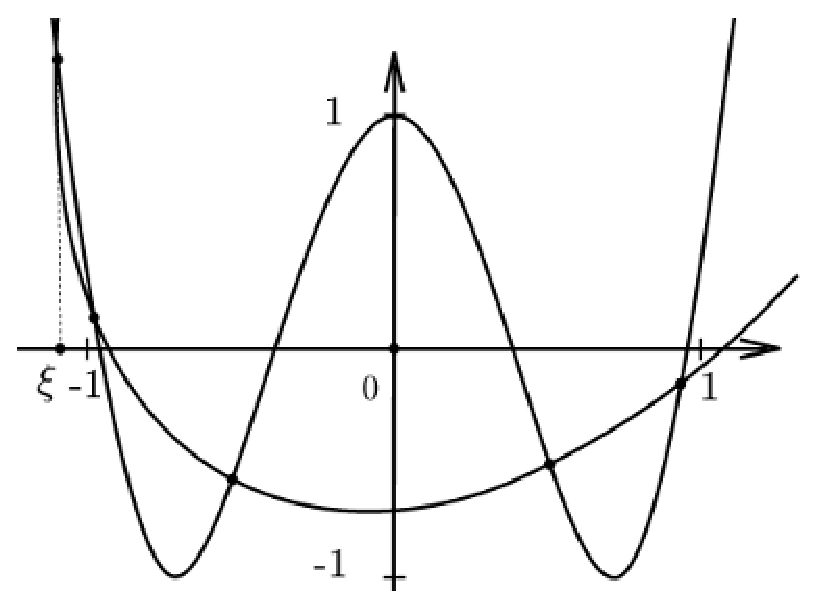
\includegraphics[width=0.34\textwidth]{pict02-3.eps}
\end{picture}
\vspace{5mm}
\refstepcounter{ris}\label{r2-3}
\end{center}

\centerline{\normalsize Рис.~\theris}


%%%%%%%%%%%%%%%%%%%%%%%%%%%%%%%%%%%%%%%%%%%%%%%%%%%%%%%%%% %\noindent \hskip3.0cm {рис. 9}

%\centerline{рис.9}


\noindent

{Далее, график полинома $y{(x)}=\dfrac{p(x)}{\|p\|_{C}}$ на отрезке
$[-1,1]$ не выходит за полосу $|y| \le 1.$ Поэтому, рассуждая как при
доказательстве теоремы~\ref{teo1extsvo}, получаем, что $q(x)$ имеет на
$[-1,1]\quad n$ нулей с учетом их кратности. Если к тому же $\xi_0 < -1$
{(см. рис.~\ref{r2-3})}, то получаем $q(x) \equiv 0$ на $\bR.$
Если же $\xi_0=-1$ и $q(x) \ne 0$ на промежутке $[\xi, -1),$ то рассуждать
нужно чуть потоньше. Во-первых, может оказаться, что $\xi_0=-1$~-- нуль
второго порядка~-- двойной корень $q.$ Ясно, что один из них не вошел в
число учтенных $n$ нулей на отрезке $[-1,1],$ так как из двойных нулей
были учтены только совпадающие с некоторыми из $\widetilde x_k=\cos
\dfrac{k\pi}{n}$~ $(k=1,2,\ldots,n-1).$}

{Вторая возможность~-- $q'(\xi_0) \ne 0$ {$(\xi_0=-1)$.}
Тогда $q(x)$ в
точке $\xi_0=-1$ меняет знак с $+$ на $-$, график $p(x)$ в
правой полуокрестности точки {$\xi_0$} окажется ниже
графика~$T_n.$ Следовательно в обоих случаях {на промежутке $[-1,\widetilde{x}_{n-1}]$}
{у полинома $q(x)$ будет не менее двух нулей,} общее число
нулей будет $\ge n+1.$ Значит, опять $q(x) \equiv 0$ на $\bR,$
что противоречит предположению.}

{Общий случай (без предположений $\xi < -1$ и $n$~-- четное) сводится к
рассматриваемому заменой $p$ и $T_n$ на $-p,\ -T_n$ и/или $T_n(x)$ на $T_n(-x)$. Лемма
доказана.}

%\end{proof}


{Таким образом, если $\|p_n\|_{C[-1,1]} \le 1,$~ $p_n \in \Cal P_n,$ и
$|\xi|>1,$ то $|p_n(\xi)| \le |T_n(\xi)|.$}

\ex {Доказать, что если $p \in \Cal P_n$ и}
$\|p(\cdot )\|_{C[-1,1]} \le 1,$ то $|p'(1)| \le T_n'(1)$ (для доказательства
опять считаем нули), {см. рис.~\ref{r2-4}}.

{Имея ввиду это свойство, $T_n$} называют многочленом сравнения.

%%%%%%%%%%%%%%%%%%%%%%%%%%%%%%%%%%%%%%%%%%%%%%%%%%%%%% %\hbox to 0.5cm {}{\special{em:graph pict10.pcx}} %\vspace{6cm} \vspace{5mm}
%\begin{picture}(100,170)
% \put(100,160){\special{em: graph pict2-4.pcx}}
% \end{picture}
% \refstepcounter{ris}\label{r2-4}

% \centerline{Рис.~\theris }
% \bigskip


 \bigskip
\begin{figure}[ht]
\begin{center}
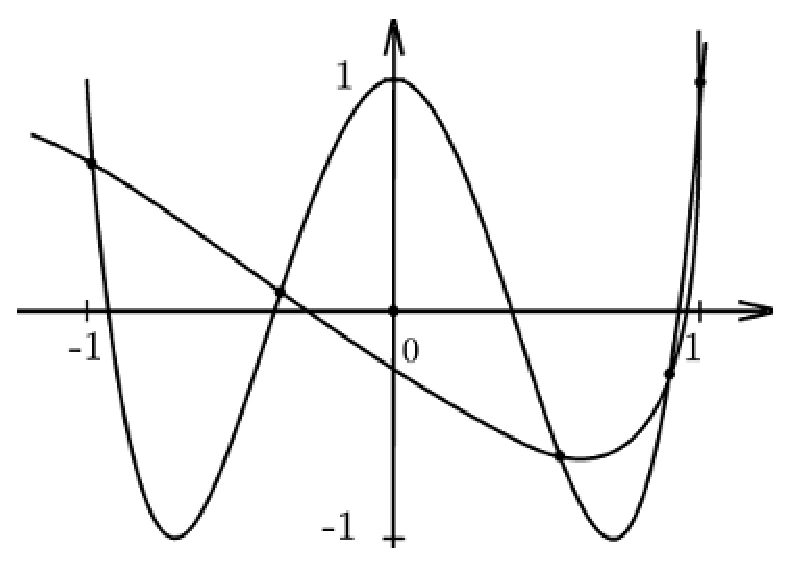
\includegraphics[width=0.35\textwidth]{pict02-4.eps}
\end{center}
 \bigskip
 \refstepcounter{ris}\label{r2-4}

 \centerline{Рис.~\theris}
 \bigskip
\end{figure}




\begin{Remark}
Из леммы~2.2 следует, что если $[-a,a] \supset [-1,1]$
 и $p_n \in \Cal P_n,$ то справедливо неравенство
\[
  \|p(\cdot )\|_{C[-a,a]} \le \|T_n(\cdot )\|_{C[-a,a]}\cdot \|p(\cdot )\|_{C[-1,1]},
\]
{где знак равенства возможен только при $p(x)\equiv 0$ или $p(x)\equiv\pm T_n(x)
\|p(\cdot )\|_{C[-1,1]}$.}
\end{Remark}

 % ���樨 ��ࣥ� ���ᮢ�� ��窨��
% ���ᥭ� ��ࠢ����� �.�.�㡡�⨭� � �.�.�����, ����� 30.06.2009
% ���ᥭ� ��ࠢ����� �.�.�����, ����� 29.07.2009
% ���ᥭ� �ࠬ����᪠� � ���-�ࠢ�� �.����������, ����� 05.08.09

\chapter{�����童�� ����襢� (�த�������).\\ {���௮���� (�ਫ������)}}  %%{����� 3.}

{\section{���६� �.\,�.\,��મ�� }}

{\bf 1. ���� ����६��쭮� ᢮��⢮ �����童��� ����襢�}

\ \

���ᬮ�ਬ ������ �.\,�.\,��મ��. �� 䨪�஢����� {$m\in \bN$ � $n \ge m$}
�।� ��� �����童��� �⥯���
{$n$ � �����樥�⮬} $a_m=1,$ ����� �����童� ��������
㪫������ �� ��� {�� $[-1,1]$}?


��� �� �襭�� �।���⥫쭮 ������� ᫥������ �����.

\begin{lemma}[����� � ����]\label{l2-3}
����� ��� {�⫨�� �� ⮦���⢥����� ���} $(N+1)$-童��� �������
$\sum\limits_{k=0}^{N}A_kx^{\lambda_k},$ $0 \le \lambda_0 < \lambda_1 < \cdots <
\lambda_N.$ ����� �� $(0,\infty )$ �� ����� ����� �� ����� $N$ �㫥�.
\end{lemma}

 %\begin{proof}
�\;�\;�\;�\;�\;�\;�\;�\;�\;�\;�\;�\;�\;�\ \ ����樥� �� $N.$
�� $N=0$ {� $A_0 \ne 0$} {�������} $A_0 x^{\lambda_0}$
�� ����� �㫥� �� $(0, \infty ).$ �� $N=1$ {� $|A_0|+|A_1|
\ne 0$ �������} $A_0 x^{\lambda_0}+A_1
x^{\lambda_1}=x^{\lambda_0}
                                   (A_0+A_1 x^{\lambda_1-\lambda_0})$
����� ����� �� ����� ������ ��� ��~$(0,\infty).$ �����
{�� $(N+1)$-童��� �������
$\sum\limits_{k=0}^{N}A_kx^{\lambda_k} \not \equiv 0$ } �����
�� ����� $N$ �㫥� ��~$(0, \infty).$ �����
{$G(x)=\sum\limits_{k=0}^{N+1}A_kx^{\lambda_k}=
                        x^{\lambda_0}\sum\limits_{k=0}^{N+1}A_kx^{\lambda_k-\lambda_0}=
                        x^{\lambda_0}\cdot F(x)$}
����� �⮫쪮 �㫥� �� $(0, \infty ),$ ᪮�쪮 �� �����
$F(x)=\sum\limits_{k=0}^{N+1}A_kx^{\lambda_k-\lambda_0},$
�� �⮬ ����� �����, �� $A_{N+1} \ne 0$ {(����
$G(x)$~-- $(N+1)$-童��� �������).} �� {⮣��}
$F'(x)=\sum\limits_{k=1}^{N+1}B_kx^{\lambda_k-\lambda_0-1}$~-- {$(N+1)$}-童���
{�� �ਢ�����} �������
{$(B_{N+1}=(\lambda_{N+1}-\lambda_0) A_{N+1}\ne 0)$}, ����� ��
�।��������� ����樨 ����� �� ����� $N$ �㫥�. �������⥫쭮,
{�� ⥮६� �����} $F(x)$ ����� �� ����� $N+1$ �㫥�. �����
��������. %\end{proof}

������ ��୥��� � ����� �.\,�.\,��મ��.

����� $C=C[-1,1],$~ $p_n \in {\Cal P}_n,$~ $p_n(x)=\sum\limits_{k=0}^{n}a_kx^k,$~
${\Cal Q}^m_{n}=\{p_n(x):\ p_n\in {\Cal P}_n,\ a_{m}=1\}.$

%\begin{task}
�ॡ���� ���� $p_n^* \in \Cal P_n$
⠪��, ��
\[
  \inf_{p_n \in {\Cal Q}^m_n} \|p_n(\cdot)\|_{C[-1,1]} =
  \min_{p_n \in {\Cal Q}^m_n} \|p_n(\cdot)\|_{C[-1,1]} =
  \|p^*_n(\cdot)\|_{C[-1,1]}.
\]
��� ������ ����� ⠪�� ��ᬠ�ਢ��� ��� ������ �
������襬 �ਡ�������, ������
\[
  \inf_{p_n \in {\Cal Q}^m_n} \|p_n(\cdot)\|_{C[-1,1]} =
  \inf_{q \in {\Cal P}_n,\ a_m=0} \|x^m-q(x)\|_{C[-1,1]} =
  E(x^m,L_n^m)_{C[-1,1]},
\]
��� $L_n^m=\{p\in {\Cal P}_n:\ a_m=0\}$ -- ����筮��୮� �������� �������࠭�⢮ ����࠭�⢠
$C,$ ���஥ �������� ��� � ${\Cal P}_n$ ᢮��⢮�: �᫨ ���쬥�
���� ��� ������ ���� ������-����� �����童�� �� �⮣�
�������࠭�⢠, � ᭮�� ����稬 �����童� �� �⮣� �������࠭�⢠.
%\end{task}

����⨬, �� �।� �����童��� {� $a_m=0$}, ����� �ਡ������ �㭪�� $x^m$
������訬 ��ࠧ��, {�������� ������訩} �����童� {⮩ ��
�⭮��, ��} $x^m$.

����⢨⥫쭮, ����� $m$ �⭮� � $p_n(x)$~-- ������訩 �����童� �� ��襣�
�������࠭�⢠. ����� {$q_n(x)=\dfrac{1}{2}\{p_n(-x)+p_n(x)\}$}
⮦� �����童� �� ⮣� �� �������࠭�⢠, �� 㦥 ���, � �ਡ������
{�㭪�� $x^m$} �� �㦥:
\[
  \|x^m-q_n(x)\|_C=\Bigl\|\frac{1}{2}(x^m-p_n(x))+
                     \frac{1}{2}((-x)^m-p_n(-x))\Bigr\|_C \le
  \|x^m-p_n(x)\|_C.
\]
�������⥫쭮, ��� �㭪樨 �ਡ�������� ��묨
�����童���� ������訬 ��ࠧ��. ��������� �뢮� ����� ᤥ���� ��� ������
�㭪権 � ������ �����童���. ��� ᫥���, � ��⭮��,
�� �᫨ $m$ � $n$ ࠧ��� �⭮��, � ������訩 �����童�
{$q_n^*$} ⮩ �� �⭮��, �� � $m$, ������ ����� �⥯���
$n-1,$ � ᫥����⥫쭮, {$q_n^*\equiv q_{n-1}^*.$}

 ������ � ��ᬮ�७�� {᫥���饥 �।�⠢����� �����童��}
����襢�:
\[
  T_n(x)=\cos{( n \arccos x)} =\sum\limits_{k=0}^n A_k^nx^k.
\]
\begin{teo}[{�.\,�.\,��મ�}]
�᫨ $m$ � $n$ ����� ���������� �⭮���, � �।� ��� �����童��� �⥯��� $n$ �
�����樥�⮬ $a_m=1$ {$(0\le m\le n)$} �������� 㪫������ ��
��� �����童� $\dfrac{T_n(x)}{A_m^n},$ � 㪫�������
\[
  \Bigl\|\frac{T_n(\cdot )}{A_m^n}\Bigr\|_{C[-1,1]}=\frac{1}{|A_m^n|}.
\]
�᫨ �� $m$ � $n$ ����� ࠧ��� �⭮���, � �।� ��� �����童��� �⥯��� $n$ ������
$a_m=1$ {$(0\le m\le n-1),$} �������� 㪫����騬�� �� ��� ���� �����童�
$\dfrac{T_{n-1}(x)}{A_m^{n-1}},$ � 㪫�������
\[
  \Bigl\|\frac{T_{n-1}(\cdot )}{A_m^{n-1}}\Bigr\|_{C[-1,1]}
                                             =\frac{1}{|A_m^{n-1}|}.
\]
\end{teo}

\begin{proof}
��� ������⥫��⢠ ���� ��ᬮ���� 4 ���� ��� $m$ � $n$ ࠧ��� �⭮�⥩. �������
{⥮६� ⮫쪮 � ����� ��砥}, ����� $m$ � $n$ ���. �⠪, ���� ��������, �� �᫨
$p_n(x)=\sum\limits_{k=0}^n a_kx^k$~-- �ந������ �����童� � $a_m=1$ {� ��묨
$n$ � $m,$} �
\[
  \| p_{n}(\cdot ) \|_{C[-1,1]} \ge \frac{1}{|A_m^{n}|}.
\]


����� �� �⢥ত���� ����୮, �.\,�. ����� ������� �����童�
{$p_n(x)$} ⠪��, ��
\begin{equation}
\label{Macar}
  \| p_{n}(\cdot ) \|_{C[-1,1]} {<} \frac{1}{|A_m^{n}|}.
\end{equation}
{�����童�} $p_n$ ����� {��} ���� ���, �� ⮣�� {$\dfrac{1}{2}(p_n(x)+p_n(-x))
\in \Cal Q^m_n$} ⮦� 㤮���⢮��� ��ࠢ�����~(\ref{Macar}) � �㤥� ���.
{���⮬� ����� ��⠥�, �� �~(\ref{Macar}) $p_n$ --} {��� �����童�, �⫨�� ��
$\dfrac{T_n(x)}{A_m^n}$.} �����童� ����襢� $T_n(x)$ ⮦� ���. ���ᬮ�ਬ �����童�
\[
  R_{n}(x)=\frac{T_n(x)}{A_m^{n}}-p_n(x)=
  \sum\limits_{k=0}^{n/2}b_kx^{2k}{\not\equiv 0,}
\]
{���} $b_{m/2}=0.$ ����� ��ࠧ��, � $R_n(x)$ �� �����, 祬 $n/2=l$ �� ࠢ��� ���
�����樥�⮢. �� {�����~\ref{l2-3}} � ���� $l$-童��� �������
{$R_n(x)\not\equiv0$} ����� ����� �� $(0,\infty)$ �, ᫥����⥫쭮, �� $(0,1)$ -- ��
����� $l-1$ �㫥�. � ��� �� $T_n(x)$ ����� �� $[0,1]$ ஢�� $n/2+1$ �祪
{$\widetilde{x}_k=\cos\dfrac{k\pi}{n} \
 \left(k=0,1,\ldots,\dfrac{n}{2} \right)$} ���ᨬ��쭮�� 㪫������, � ������
$R_n(x)$ {� ᨫ�~(\ref{Macar})} ����� �� �� ����, �� � $\dfrac{T_n(x)}{A_m^{n}}$ �,
�����, ����� ���� ���� $n/2=l$ �祪, � ������
$R_n(x)=0.$ �� �� $l$ �㫥� $R_n(x)$ ����� �筮 � {���ࢠ��} $(0,1),$
{�� ��⨢���� �।��饬� �뢮��.} �������⥫쭮, �����~(\ref{Macar})
����� ��⨢��������� ��ࠢ���⢮, ���஥ ���頥��� � ࠢ���⢮ ��
$p_n(x)\equiv\dfrac{T_n(x)}{A_m^{n}}.$ � ��⠫��� ����� ⥮६�
�����뢠���� �������筮.
\end{proof}

\begin{Remark}
� ��饬 ��砥 �����童� �������襣� 㪫������ ��
�����⢥���. ���ਬ��, �� $n=2,$ $m=0$ � $0\le c\le 2$
�����
{$$
\|1-cx^2\|_{C[-1,1]}=1=\left\|\dfrac{T_2(x)}{A_0^2}\right\|_{C[-1,1]}.
$$}
\end{Remark}



\begin{Corollary}[�業�� �����樥�⮢ �����童���]
����� $p_n(x)=\sum\limits_{k=0}^n a_kx^k$ � �����⭠ ��ଠ
$\|p_n(\cdot )\|_{C[-1,1]}.$ ����� ��� $m$ � $n$ ����������
�⭮��
\[
  |a_m| \le |A_m^n|\cdot  \|p_n(\cdot )\|_{C[-1,1]},
\]
{�} ��� $m$ � $n$ ࠧ��� �⭮��
\[
  |a_m| \le |A_m^{n-1}|\cdot  \|p_n(\cdot )\|_{C[-1,1]}.
\]
\end{Corollary}

\begin{proof} ����⢨⥫쭮, ���ਬ��, ��� $m$ � $n$ {����������}
{�⭮�� � $a_m\neq 0$} �� ⥮६� ᫥��� {�業��}
\[
  \Bigl\| \frac{p_{n}(\cdot )}{a_m} \Bigr\|_{C[-1,1]}
  \ge \frac{1}{|A_m^{n}|},
\]
�, �����, � �ॡ㥬�� ��ࠢ���⢮. {�� $a_m=0$ �� ��ࠢ���⢮ �ਢ���쭮�.}
�������⥫쭮, � �����童��� ����襢� �����樥��� ����������
� �⥯���� �����童�� �⭮�� ᠬ� ����訥
{�।� �����童��� $p_n$ ⮩ �� �⥯��� � $\|p_n\|_{C[-1,1]}\le 1.$}

\begin{ex}
�஢��� ������⥫��⢮ ⥮६� ��મ�� ��� $m$ � $n$
ࠧ��� �⭮��.
\end{ex}
\end{proof}

\begin{Remark} ��� ��� $a_m={\dfrac{p_n^{(m)}(0)}{p!}}$,
� {��ࠢ���⢠ ᫥��⢨� ����� ��९����} {� ����}
\[
  |p_n^{(m)}(0)| \le m!\cdot |A_m^n|\cdot  \|p_n(\cdot )\|_{C[-1,1]},
\]
\[
{|p_n^{(m)}(0)| \le |T_n^{(m)}(0)|\cdot \|p_n(\cdot )\|_{C[-1,1]}\qquad (0\le m\le n)}
\]
��� $m$ � $n$ ���������� �⭮�� �
\[
  |p_n^{(m)}(0)| \le m!\cdot |A_m^{n-1}|\cdot  \|p_n(\cdot )\|_{C[-1,1]},
\]
\[
{|p_n^{(m)}(0)| \le |T_{n-1}^{(m)}(0)|\cdot \|p_n(\cdot )\|_{C[-1,1]} \qquad (0\le m\le n-1)}
\]
���
$m$ � $n$ ࠧ��� �⭮��.
\end{Remark}
%\end{proof}

\section{����६��쭠� ���௮���� �� ����� $W^{n+1}$}

{\bf 1. ��⢥�⮥ ����६��쭮� ᢮��⢮}

\ \

����� $a \le x_0<x_1<\dots <x_n\le b$~-- 㧫� ���௮��樨 ��
$[a,b],$ $f \in \G M \subset C^{(n+1)}[a,b]$,~ $p_n(x,f)=\sum\limits_{k=0}^n
f(x_k)l_k(x)$~-- ���௮��樮��� �����童� ���࠭��. �����, ��� �� �����,
\[
  R_n(x,f)=f(x)-p_n(x,f)=\frac{f^{(n+1)}(\xi)}{(n+1)!} \omega (x),
\]
��� $\xi \in [a,b]$ � $\omega(x)=(x-x_0)\cdots (x-x_n).$
�⠪, ����� ����� �㭪権 $f \in \G M.$
��� �������� 㧫� ⠪, �⮡� ���⮪ ���௮��樮���� ���� �� �ᥬ� ������ ��
�������訩?


��� ����� $\G M$
��ᬮ�ਬ ����稭�
\begin{equation}
\label{estim1}
  \sup_{f \in \G M}\| R_{n}(\cdot ,f,\{x_k\}) \|_{C[-1,1]}
                      =F_n(\G M,\{x_k\}),
\end{equation}
{���� $[a,b]=[-1,1]$.} ����� �⠢���� ⠪: ��� ����� 㧫�,
�⮡� ����稭�~(\ref{estim1}) �뫠 �������, �.\,�. ���� ����
\[
  \inf_{\{x_k\}}F_n(\G M,\{x_k\})=\Phi_n(\G M).
\]
{�����} ��� �� �㭪樨 $f \in \G M $ {� ����६����� 㧫�� �㤥� �����}
$$
{\| R_{n}(\cdot ,f,\{x_k\}) \|_{C[-1,1]} \le \Phi_n(\G M).}
$$

����⨬, �� �᫨ ��� �������� �㭪樨 �롨��� 㧫� ⠪, �⮡� ����稭�
$\|f(\cdot )-p_n(\cdot ,f)\|_{C[-1,1]}$ �뫠 �������襩, � �� �뫠 ��
{\it ��㣠� �����}. �� �� ����� �� �蠥�.

�롥६ � ����⢥ $\G M$ �����
\[
 W^{(n+1)}=\{f{\in C^{n+1}[-1,1]}:\ \|f^{(n+1)}\|_{C[-1,1]}{\le 1}\}.
\]
������
\[
  \inf_{\{x_k\}}\sup_{f \in W^{(n+1)}} \| R_{n}(\cdot ,f,\{x_k\}) \|_{C[-1,1]}.
\]
��䨪��㥬 $x \in [-1,1].$
�� ���� ��� ����筮�� 童�� � �ଥ ���
\[
   R_n(x,f)=\frac{f^{(n+1)}{(\xi )}}{(n+1)!} \,\,\omega (x)
\]
᫥���
\[
  \sup_{f \in \,W^{(n+1)}} | R_{n}(x ,f,\{x_k\}) | \le \frac{|\omega(x)|}{(n+1)!}.
\]
��� ��� ������� �㭪��, ��� ���ன $f^{(n+1)}(x) \equiv \pm 1,$ ���ਬ��,
�᫨ $f$ ���� �����童� � ���訬 �����樥�⮬ $\pm
\dfrac{1}{(n+1)!},$ � �� �業�� ���頥��� � ࠢ���⢮ ��� ��� $x \in [-1,1]$:
\[
  \sup_{f \in \,W^{(n+1)}} | R_{n}(x ,f,\{x_k\}) | =\frac{|\omega(x)|}{(n+1)!}.
\]
�����, �
\[
  \sup_{f \in\, W^{(n+1)}} \| R_{n}(\cdot ,f,\{x_k\}) {\|}_{C[-1,1]} \le
                                \frac{\|\omega(\cdot )\|_{C[-1,1]}}{(n+1)!},
\]
��祬 {���� ࠢ���⢠ �㤥�} ����� ��� ⮩ �� �㭪樨.
�������⥫쭮, ����� ᢥ���� � ��宦�����
\[
  \inf_{\{x_k\}} \|\omega(\cdot )\|_{C[-1,1]}.
\]
��� ��� $\omega (x)=\prod\limits_{k=0}^n (x-x_k)=x^{n+1}+\cdots ,$ �
\[
  \inf_{\{x_k\}} \|\omega(\cdot )\|_{C[-1,1]} \ge
  \inf_{x^{n+1}+\cdots } \|p_{n+1}(\cdot )\|_{C[-1,1]}
  =\|\widetilde T_{n+1}(\cdot )\|_{C[-1,1]}=\frac{1}{2^{n}}.
\]
�� ᠬ�� ���� ����� {ࠢ���⢮}, ⠪ ��� ����� {��� ��ᬠ�ਢ�����} $\omega (x)$~--
{�� �����} �����童��� � ���訬 �����樥�⮬,
ࠢ�� $1$, � � ��ﬨ $x_k \in [-1,1]$\ $(k=0,\dots ,n),$ {�}
��ନ஢���� �����童� ����襢� {$\widetilde{T}_{n+1}$} ����� � �⮬
�����. �������⥫쭮,
\[
  \inf_{\{x_k\}}\sup_{f \in W^{(n+1)}} \| R_{n}(\cdot ,f,\{x_k\}) \|_{C[-1,1]}
  =\frac{1}{(n+1)!}\cdot 2^{-n}
\]
� ���⨣����� ��� {㧫��} $\{x_k\},$
������ ��ﬨ $T_{n+1}.$

\begin{task}
����
$$
\inf\limits_{\{x_k\}}\sup\limits_{f \in W^{(r)}}
             \| R_{n}(\cdot ,f,\{x_k\}) \|_{C[-1,1]}
$$
��� ��� $0 \le r \le n+1.$
\end{task}

��� $r=0$ ����� {�襭� �ᨬ����᪨,} ��� $r=n+1$ {�襭�� ����� �뫮} {�������� ⮫쪮
��,} ��� ��⠫��� $r$ ����� �� �襭�.

\section{���௮���� � �������᭮� ������}

���ᬮ�ਬ ���������� ���᪮��� $\bC,$ ������� {$D \subset \bC,$} � ����� $w=f(z)$~--
�������᭮���筠� �㭪�� �� $D.$ ����� � ������ $D$
������ ��⥬� ࠧ����� �祪 $\{z_k\}$ $(k=0,\dots ,n).$

����ந� �����童� $p_n(z,f)$
⠪��, �⮡�
\[
  p_n(z_k)=f(z_k).
\]
���௮��樮���� ��㫠 ���࠭�� � ����� ��࠭����:
\[
  p_n(z,f)=\sum\limits_{k=0}^n f(z_k)l_k(z),\qquad {l_k(z)=\frac{\omega(z)}{\omega'(z_k)
  (z-z_k)},\qquad
  \omega(z)=\prod_{m=0}^n(z-z_m)}.
\]
����� $f$~-- �������᪠� (ॣ��ୠ�) �㭪�� � ������ $D,$ �.\,�. �
$f$ ������� $f'$ � $D,$ � ����� $D$ �����吝�. ������ ��ࠦ���� ���
����筮�� 童��. ���ᬮ�ਬ � $D$ ������ $C$ ⠪��, �� �� �窨 $z_k$
����� ����� $C.$ �㭪�� $\dfrac{f(z)}{(z-z_0)\cdots (z-z_n)}$ �����
$C$ ����� � ����⢥ �ᮡ�����⥩ ⮫쪮 �窨 $z_0,\dots ,z_n$ � ����� ⠬
{���࠭��� �ᮡ������ (�᫨ $f(z_k)=0$) ���} ����� �����,
⠪ ��� $z_k \ne z_l$ �� $k \ne l.$ ����� {�� ⥮६� � �����}
$$
  \frac{1}{2\pi i}\int_C\frac{f(t)\,dt}{(t-z_0)\cdots (t-z_n)}
  =
$$
$$
  =\sum\limits_{k=0}^n \frac{f(z_k)}{(z_k-z_0)\cdots
                    (z_k-z_{k-1})(z_k-z_{k+1})\cdots (z_k-z_n)}
 = \sum\limits_{k=0}^n \frac{f(z_k)}{\omega'(z_k)}.
$$
��䨪��㥬 ��� $z$
����� ������ $C.$
������稬
\[
  J(z)=\frac{1}{2\pi i}\int_C \frac{f(t)\,dt}{(t-z)\prod_{k=0}^n(t-z_k)}.
\]
�����
\[
  J(z)=\frac{f(z)}{\prod_{k=0}^n(z-z_k)}-
  \sum\limits_{k=0}^n \frac{f(z_k)}{(z-z_k)\omega'(z_k)}
\]
���
%\begin{multline*}
\[
  J(z)\cdot \omega(z)=f(z)-\sum\limits_{k=0}^n
            \frac{f(z_k)\omega(z)}{(z-z_k)\omega'(z_k)}={f(z)-p_n(z,f)=}R_n(z,f)
 =\frac{1}{2\pi i}\int_C \frac{\omega(z)f(t)\,dt}{(t-z)\omega(t)}
\]
%\end{multline*}
��� ��� $z$ ����� $C.$ �।�⠢�� $f(z)$ � ���� ��⥣ࠫ� ���
\[
{f(z)=}\frac{1}{2\pi i}\int_C \frac{\omega(t)f(t)\,dt}{(t-z)\omega(t)}.
\]
����� ���௮��樮��� �����童�
\[
  p_n(z,f)=f(z)-R_n(z,f)=
 \frac{1}{2\pi i}\int_C \frac{\{\omega(t)-\omega(z)\}f(t)dt}{(t-z)\omega(t)}.
\]

\section{���⥩訥 �ਫ������\\ ���௮��樮���� ����
���࠭��}\label{3.4}


����� {�㭪�� $f$} ��।����� �� $[a,b].$ � �ਫ������� {���} ����砥���
����� � ���᫥��� ���祭�� �㭪樮����� � �����஢ �� �������� $f$
�㭪樮������ ����࠭��. ����筮, � ��饬 ��砥 �����
����� ������� ���� � �ਡ�������� ��⮤��.

%\subsubsection{1. ���᫥��� {���祭��} �㭪樮���� $F(f),$
%�.\,�.�᫠}
\vspace{3mm}
{\bf 1. ���᫥��� ��।�������� ��⥣ࠫ�}
\vspace{3mm}

����� ��ᬠ�ਢ����� �� ����� �� �ਬ�� ���⮣� �㭪樮����
$\displaystyle\int_a^b f(x)\,dx.$ �� �⮬ ��� ���⥩襣� �㭪樮����~-- ���祭�� �㭪樨 �
�窥 -- ��⠥���
������� ��� ��� �ਡ������� ��⮤ ���᫥���.

%\subsubsection{2. ���᫥��� {���祭��} ������ A(f){,
%�.\,�. �㭪樨 $A(f)(x).$}}


%\subsection{���᫥��� $\displaystyle\boldsymbol{\int_a^b f(x)dx}$}\label{3.2.1}

����� $f(x)\in C[a,b],$ $p_n(x,f)$~-- ���௮��樮��� �����童�, $\{x_k\}$~--
㧫� ���௮��樨, $\{f(x_k)\}$~-- ���祭�� �㭪樨 � 㧫��.

������ ��⥣�஢���� �㭪樨 � ��⥣�஢���� �� ���௮��樮����� �����童�� ���࠭��.
��� ��⥣ࠫ� �������� �������ୠ� ��㫠.

�⠪, �����塞 ���᫥��� $\ds\int_a^b f(x)\,dx$ ���᫥����
\begin{equation}\label{3-3.3}
  \int_a^b p_n(x,f)\,dx=\sum\limits_{k=0}^n f(x_k)\int_a^b l_k(x)\,dx=
  \sum\limits_{k=0}^n A_k f(x_k) \approx \int_a^b
  f(x)\,dx,
\end{equation}
��� $l_k(x)=l_k(x;\{x_i\}_0^n),\ A_k=A_k(n).$
�� ��㫠 ���뢠���� �������୮� ��㫮� {����}, $\{x_k\}^n_{k=0}$~-- 㧫�
�������୮� ����, $\{A_k^n\}^n_{k=0}$~-- �����樥��� �������୮� ���� ���
�����樥��� ����.

�ᮡ�������� ⠪�� ��� ���� �, �� ��� ��� ��� ��� ��������� �⥯��� �� ��� $n,$
�.\,�. �᫨ $f$ ���� �����童� �⥯��� �� ��� $n,$ � ⠪�� ��㫠 �㤥�
�筮�, � {�� �ࠢ�� ���} �㤥� ���� ࠢ���⢠.

��� ⮣� �⮡� ��㫠~(\ref{3-3.3})
�뫠 �筠 ��� ��� �����童�� �⥯��� �� ��� $n,$ ���
������ ���� �筠 ��� �㭪権 $x^p$\ $(p=0,1,\dots ,n).$

�����, �����樥��� ���� ����� �����:
\[
  \sum\limits_{k=0}^n A_k x^p_k=\int_a^b x^p dx\qquad (p=0,1,\dots ,n).
\]
�� ��⥬� � ��।���⥫�� �����ମ���, �~$A_k$ ��।������� �������筮.

��������� ��ࠧ�� ����� �ᯮ�짮���� ���௮��樮���
�����童�� ���࠭�� ��� �ਡ��������� ���᫥��� ���祭��
��㣨� �������� �㭪樮�����. �業�� ����譮��
ᮮ⢥������� ���������� ��� ��ࠦ����� �१ ����
�㭪樮����� � �業�� ����譮�� ���௮��樮���� ���.

\begin{ex}
�믨��� ⠪�� �業�� ��� ���������� ���, �ᯮ����
१����� �� �।���� ���権.
\end{ex}

����� ��ந�� �㡠���� ����, ���� �᫨
���௮��樮��� ���� ������� �����. ���ਬ��, ��� �㭪権 ��᪮�쪨� ��६�����
�� �㡥, ��� ����� ��� �����뢭�� ���௮��樮����
��⥬, ����� ����ந�� �㡠���� ���� ��� �� �����童��� �������� �⥯���.
\vspace{3mm}

{\bf 2. ���᫥��� {���祭��} ������ ${A(f)},$
{�.\,�. �㭪樨 ${A(f)(x)}$}}
\vspace{3mm}

��������� �ਥ� ����� �ᯮ�짮���� ��� �ਡ���������
���᫥��� ���祭�� ��������� ������, �᫨ 㬥��
�������~$A(l_k)(x).$ ��� ����࠭�祭��� �����஢ �� ��
�ࠡ�⠥�. ���ਬ��, ���쬥�
�����쭮 ���⮩ ����⨢�� � ����த�� ������~-- ������ ����७�஢����.
����� ���᫥���~$f'(x)$ �� ����筮�� ��� �祪 {���
�������⥫쭮� ���ଠ樨 �} {�㭪樨 � �� �ந�������} �� ����� ��᫠,
⠪ ��� ������ ����७�஢���� �� ��࠭�祭 � ����� �����뢭��
�㭪権, {� ����� �� 㤠���� 㪠����} {��࠭�஢����� ����譮���
�ਡ�������� ���� ���~$f'(x).$} ������ ����७�஢����
����� ᤥ���� �����뢭� �� �������࠭�⢥ $C^{(r)}[a,b]\subset C[a,b]$ �㭪樨 �
�����뢭�� �ந������� ���浪� $r,\ r\ge 2$, �᫨
����� � $C^{(r)}[a,b]$ ���� ᮡ����᪮�� ⨯�,
�������
$$
\|f\|=\|f\|_{C[a,b]}+\|f^{(r)}\|_{C[a,b]}.
$$
��࠭�祭����� �����஢ ����७�஢���� ���浪�
$1,2,\ldots,r-1$ ����� �������, �ᯮ����, ���ਬ��, ���� ������
� ������ 童��� � �ଥ ��� � ᫥��⢨� �� ��ࠢ���⢠ ���쥢 ��મ���
��� �����ࠨ�᪨� �����童��� $p_n(x)$
$$
\|p_n^{(k)}\|_{C[a,b]}\le \dfrac{2^{k}}{(b-a)^k}  n^{2k}\|p_n\|_{C[a,b]}.
$$
� ��砥 ��ਮ���᪨�
�㭪権 � �㭪権, ��।������� �� $\mathbb R,$
��࠭�祭����� ��� ����७樠���� �����஢ ��
����࠭�⢠� $C^{(r)}_{2\pi}$ � $C^{(r)}(\mathbb R)$ �
ᮡ����᪮� ��ମ� ��⥪��� �� ᮮ⢥������� ��ࠢ���� �������஢�, �����
���� ���㦤����� � ���쭥�襬\footnote{� ������ 19 (�.~19.4) � 20 (�.~20.1).}.

 % ���樨 ��ࣥ� ���ᮢ�� ��窨��
% ���ᥭ� ��ࠢ����� �.�.�㡡�⨭� � �.�.�����, ����� 30.06.2009
% ���ᥭ� ��ࠢ����� �.�.�����, ����� 29.07.2009
% ���ᥭ� �ࠬ����᪠� � ���-�ࠢ�� �.����������, ����� 05.08.09

\chapter{��������� ������\\ � ���௮��஢���� � �ந�����묨}
%%{����� 4.}

\section{��������� ����}

� �㭪樮���쭮� ����࠭�⢥  $B$ � ��।�����묨 ���� �� $[a,b]$ �㭪�ﬨ
$f\in B$ � ��ମ� $\|f\|$
��ᬮ�ਬ ���������� ����
\begin{equation}
\label{Quad}
  \Cal L(f)=\sum\limits_{k=1}^n A_kf(x_k)
\end{equation}
��� �ਡ��������� ���᫥��� ������-� �㭪樮����. ����� � ����� $A_k=A_k(n,\Cal
L),$ $\{x_k\}_{1}^n$ -- ����� ࠧ����� �祪 �� $[a,b].$

�������ୠ� ��㫠 �㤥� ������� �㭪樮�����, �᫨ ���祭��
�㭪樨 � �窥 ���� ������� (�.\,�. ����⨢��,
����த�� � ��࠭�祭��) �㭪樮���. �᭮, �� $\Cal
L$~-- {�������} �㭪樮���, �᫨ $B=C[a,b].$ ���筮 ���������
���� ��ᬠ�ਢ��� � ����� �㭪権, ᮢ�����騬 ���� �
ᠬ�� ����࠭�⢮� $C[a,b],$ ���� �
{����} ���ਧ������ �������࠭�⢮� $B$ �⮣� �� ����࠭�⢠, ���ਬ��,
$B=C^{(r)}[a,b]$ � ��ମ� �������� $\|f\|=\|f\|_{C[a,b]}+\|f^{(r)}\|_{C[a,b]}.$

����� ��ࠧ��, �� �㤥� ��ᬠ�ਢ��� ��������� ����
� ����࠭�⢠�, � ������ ���祭�� �㭪樨 � �窥
���� ������� �㭪樮���.

1. �� �������ୠ� ��㫠, �᫨ �� ��ᬠ�ਢ��� �
����࠭�⢥, ��� ��� ���� ������� �㭪樮���, �����
����
\[
  \|\Cal L \|=\sup_{\|f\| \le 1} |\Cal L (f)|
\]
-- �� �� ��ࢠ� �ࠪ���⨪�. � ����࠭�⢥ {$C[a,b]$}
����砥� �業��
\[
 \|\Cal L \|_{C} \le
              \sum\limits_{k=1}^n |A_k|
\]
� ࠢ���⢮ ����� ���� ��� {$f \in C[a,b]$} ⠪��, �� $f(x_k)=\sign A_k.$ �����
�㭪�� �ᥣ�� ������� (�. ��.~\ref{r4-1}).

%%%%%%%%%%%%%%%%%%%%%%%%%%%%%%%%%%%%%%%%%%%%%%%%%%%%%%
%\vspace{3mm}
% \noindent

 %\bigskip
 %\begin{picture}(90,130)
 %\put(90,130){\special{em: graph pict4-1.pcx}}
 %\end{picture}

 %\refstepcounter{ris}\label{r4-1}

 %\centerline{���.~\theris}
 %\bigskip

  \bigskip
\begin{figure}[ht]
\begin{center}
\includegraphics[width=0.7\textwidth]{pict04-1.eps}
\end{center}
 \bigskip
 \refstepcounter{ris}\label{r4-1}

 \centerline{���.~\theris}
 \bigskip
\end{figure}



%%%%%%%%%%%%%%%%%%%%%%%%%%%%%%%%%%%%%%%%%%%%%%%%%%%%%%%%%%
%\vspace{1mm}
%\noindent\centerline{\hspace{-6cm}��.11}

%\hbox to 0.5cm {}{\special{em:graph pict11.pcx}}
%\vspace{4.6cm}
%%%%%%%%%%%%%%%%%%%%%%%%%%%%%%%%%%%%%%%%%%%%%%%%%%%%%%%%%%
%\noindent \hskip3.0cm {��. 11}
%\bigskip

\noindent �������⥫쭮,
\[
 \|\Cal L \|_C=\sum\limits_{k=1}^n |A_k|.
\]
�᫨ �� ���᫥��� ���祭�� $f(x_k)$ �㭪樨 $f$
�� �訡���� �� $\e,$ � � �������୮� ��㫥 �� �訡����
�� �����, 祬 �� $\e \sum\limits_{k=1}^n |A_k|.$

2. ���� �ࠪ���⨪� �������୮� ����~-- �������
�筮�� �������୮� ����.
�������ୠ� ��㫠~-- ���᫨⥫�� ��⮤ ���
��宦����� ���祭�� ������-� �㭪樮����, ���ਬ��, �㭪樮����
\[
  M(f)=\int_a^b f(x) \,dx.
\]
����� ������, $M(f) \ne \Cal L(f).$
������ ��� �� �������୮� ���� � ᮮ⢥�����饣�
�㭪樮���� $M$ ������� ������⢮
$\Cal Q$ ⠪��, ��
\[
  M(f) = \Cal L(f) \qquad \forall f \in \Cal Q.
\]
�� ������⢮ $\Cal Q$ ���뢠���� {\it �������� �筮�� �������୮� ���� ���
$M(f)$.}

��� �� �������୮� ���� ������� �筮�� ��
���� (⠪ ��� ⮦���⢥��� ��� �ᥣ�� ����� �
$\Cal Q$) � � ����� ����� ����� ᮢ������ ���� � �ᥬ ����࠭�⢮�.

\begin{defi}
�᫨ ��� �����ண� $m,$ $\Cal P_m \subset \Cal Q,$ {a $\Cal
P_{m+1}\not\subset \Cal Q,$} � �㤥� �������, �� {\it
�������ୠ� ��㫠 ����� �筮��� $m.$}
\end{defi}

� ��⭮��, �������ୠ� ��㫠 ����� �筮��� $m=0$ ��� $M(f),$
�᫨ ��� �� ����ﭭ�� $c$
�믮����� $M(c) = \Cal L(c)=c\cdot \sum\limits_{k=1}^n A_k$
{� $M(f)\ne\sum{A_kx_k}$ �� $f(x)\equiv x$}.
�᫨ $
M(f)=\displaystyle\int_a^b f(x)\, dx,$ � $M(c)=(b-a)c$
{� ��� �筮�� $m=0$ �������୮� ����~(\ref{r4-1})}
����室��� � �����筮, �⮡�
\[
  \sum\limits_{k=1}^n A_k=b-a\quad \mbox{�}\quad \sum\limits_{k=1}^n
  A_kx_k\ne\frac12(b^2-a^2).
\]
��ࢮ� �� ��� ��ࠢ���� ���� ����室��� �
������� ��� ⮣�, �⮡� ��㫠~(\ref{r4-1}) ��� �㭪樮����
$\displaystyle\int_a^b f(x)\, dx$ ����� �筮��� $m\ge 0.$
� ��饬 ��砥 �筮��� �� �������୮� ���� �㤥� �� �����
$m,$ �᫨ ��� �筠 ��� $1,x,x^2,\ldots,x^m.$

\section{��������� ������ � �� �室������}

�᫨ � ����࠭�⢥
{$C[a,b]$} ������ ������� �㭪樮���
$M(f)$ � ��᫥����⥫쭮��� ���������� ���
$\Cal L_n$\  $(n \in \bN),$ � ����ਬ, ��
$\{\Cal L_n\}$ ��।���� ��������� �����.

\begin{task}
�� ����� �᫮���� ��� �� $f$
�� ����࠭�⢠ ��୮ ᮮ⭮襭��
\[
  \Cal L_n(f) \to M(f) \qquad (n \to \infty)?
\]
\end{task}

�� ���� �室������ �������� �㭪樮�����, ��⮬ ᫠���. �������⥫쭮, ����, �⮡�
��᫥����⥫쭮��� $\{\Cal L_n\}$ �뫠 ᫠�� �室�饩��.

\vspace{5mm}
{\bf 1. ������� �᫮��� �室����� �������୮�� �����}
\vspace{5mm}

\begin{teo}\label{kvad1}
��������� ����� �㤥� �室�騬��, �᫨

$1)$ ��᫥����⥫쭮��� ��� ���������� ���
$\{\Cal L_n\}$ ��࠭�祭�,

$2)$ $m(n) \to \infty$ {��} $n \to \infty,$
���
$m(n)$~-- �筮��� {�������୮� ����} $\Cal L_n.$
\end{teo}

\begin{proof}
{�� 㬥���� ��魮��, ����� �����, �� $m(n)$}
{�����⠥� ����� � $n.$ ����� $\Cal L_n(p)=M(p)$
��� ��� �����童�� $p(x)\in \Cal P_m$ ��} {$m(n)\ge m,$
�.\,�. $L_n(p)\to M(p)$~ $(n\to\infty)$. ���⮬�} ��� ��� $m$
��������� ����� �室���� {�� $\Cal P_m$}. �������⥫쭮, ��������� �����
�室���� �� {${\bigcup\limits_m} \Cal P_m.$} �� �� ⥮६�
���������� {$\overline{{\bigcup\limits_m} \Cal P_m}=C[a,b],$} �����, ��������� �����
�室���� �� ���� ���⭮� ������⢥, � ���� {$\|\Cal L_n\|_C$} ��࠭�祭�.
���⮬� ��������� �����
�室���� �� {$C[a,b].$}
\end{proof}

\begin{Remark}
{��������� ����� ����~(\ref{3-3.3}) 㤮���⢮��� �᫮��� 2
⥮६�~\ref{kvad1},} {⠪ ���
$m(n)=n$ (�. ࠧ���~\ref{3.4}, �.~1). �� �筮��} ���������� ��� ��
$[a,b]$ {��� ����⠭� ᫥���, �� �~(\ref{3-3.3})}
$\sum\limits_{k=1}^n A_k=b-a.$ �᫨ ��
�� �����樥��� ���� $A_k=A_k(n)$ ������⥫��, � ���� �������୮�� �����
\[
  \sum\limits_{k=1}^n |A_k|=
  \sum\limits_{k=1}^n A_k=b-a
\]
���� ��࠭�祭� {� ��������� ����� ���� �㤥� 㤮���⢮����
⥮६�~\ref{kvad1}.}
\end{Remark}

\vspace{5mm}
{\bf 2. ������� ��������� ������ � �� ������ 童��}
\vspace{5mm}

�� 㦥 ��ᬠ�ਢ��� ��������� ���� ���� ��� ���᫥���
$M(f)=\ds\int_a^b f(x)\,dx$:
\[
  \Cal L_n (f)=\int_a^b p_n(x,f)\,dx=
  \sum\limits_{k=0}^n A_k f(x_k),\qquad A_k=A_k(n),
\]
��� {$p_n(x,f)$~-- ���௮��樮��� �����童� ���࠭�� �� �⪥
$\{x_k\}_{k=0}^n\subset[a,b],$}  $A_k=\ds\int_a^b l_k(x)\,dx.$ �� �������ୠ�
��㫠 ����� �筮��� {�� �����} $n$ �
\[
  \|\Cal L_n(f)\|=\sum\limits_{k=1}^n |A_k|.
\]
����� $f \in C^{(n+1)}$
{� $\|f^{(n+1)}\|_C=M_{n+1}$}.
�����
$$
  \Bigl|  \int_a^b f(x)\,dx - \Cal L_n(f) \Bigr|=
  \Bigl|  \int_a^b (f(x) - p_n(x,f))\,dx \Bigr|=
$$
$$
  =\Bigl|  \int_a^b \frac{f^{(n+1)}(\xi )}{(n+1)!}\omega (x)\,dx \Bigr| \le
  \frac{M_{n+1}}{(n+1)!}   \int_a^b |\omega (x)|\, dx.
$$
��������� �業�� ����� ������� �१
$M_r$ ��� $0 \le r \le n+1$,
�ᯮ���� ����祭�� ࠭�� �業��~(\ref{lab1}) ��� $|f(x)-p_n(x,f)|$
�१ $\| f^{(r)}\|.$

\vspace{3mm}
{\bf 3. ��������� ���� ����ᮢ᪮�� ⨯�}
\vspace{3mm}

�� ��ᬮ�५� ���������� ���� $\sum\limits_{k=0}^n A_k f(x_k),$ ����� ����
�ਡ�������� ���祭�� ��� $\ds\int_a^b f(x)\,dx$ � �筠 ��� �� $f \in \Cal P_n.$
���㫠 ��ந��� �� 㧫�� $\{x_k\}_{k=0}^n$ � ����� $n+1$ �����樥�⮢
$\{A_k\}_{k=0}^n,$ �.\,�. ��।������ $2(n+1)$ ��ࠬ��ࠬ�.

\begin{teo}
�����
$L_{n+1}$~-- �����஥ {$(n+1)$-��୮�} �������࠭�⢮ ��
$C[a,b].$ ����� �������
{$(n+1)$-��筠�}
�������ୠ� ��㫠, ����� ����
�筮� ��� �� $f \in L_{n+1}.$
\end{teo}

\begin{proof}
����� $\phi_0(x),\dots ,\phi_n(x)$~-- ��⥬� �������
������ᨬ�� �㭪権 � $L_{n+1}.$ ����� �������� �窨 $x_i$
$(i=0,\dots ,n)$ ⠪��, ��
\[
  \det |\phi_j(x_i)| \ne 0.
\]
{(��� 䠪� ����� �������� ����樥� �� $n,$ ��砢 � $\varphi_0(x)\neqv 0$ �� $[a,b]$).}
� ����⢥ 㧫�� �������୮� ���� ���쬥� �� �窨
$\{x_i\}_{i=0}^n.$
����� ��� ��।������ $A_k$
����稬 ��⥬� �������� �ࠢ�����
\[
  \sum\limits_{k=0}^n A_k \phi_j(x_k)=\int_a^b
  \phi_j(x)\,dx,\qquad j=0,\ldots,n,
\]
�� ���ன $A_k$
��।������� �������筮 (��।���⥫� ��⥬� �� ࠢ��
���) � ��㫠 �㤥� �筠 ��� �� $f \in L_{n+1}$
(⠪ ��� $f$
������� ��ࠦ����� �१ $\phi_k,$ $k=0, \dots ,n,$
� �� $\phi_k$
��㫠 �筠).
\end{proof}

\begin{task} ����� $L_m$ {-- �������࠭�⢮ ࠧ��୮�� $m$ �� $C[a,b],$}\   $n+1<
m \le 2(n+1).$ ����� ����� ����ந�� {$(n+1)$-�����} ���������� ����, �����
�뫠 �� �筠 �� �ᥬ $L_m$?
\end{task}

�⢥� �������⥭. �᫨ �� $L_m=\Cal P_{m-1},$ � ����� �襭� ����ᮬ.

\begin{teo}[�.\,�.\,�����]
�������� 㧫� $\{x_0,x_1,\dots ,x_n\}$ {� �����樥���} $A_0,A_1,\dots, A_n$ ⠪��,
�� ��� ��� �����童�� $p \in \Cal P_{2n+1}$ �������ୠ� ��㫠 �筠, �.\,�.
\[
  \sum\limits_{k=0}^n A_k p(x_k)=\int_a^b p(x)\,dx.
\]
\end{teo}

\begin{proof}
1) ����� ⠪�� �������ୠ� ��㫠, �筠� ��� ��� $p \in \Cal P_{2n+1},$
�������. ����ந� �����童� $\omega(x)=(x-x_0)\cdots (x-x_n) \in \Cal P_{n+1}.$
���쬥� �� $q(x) \in \Cal P_{n}.$ �������, ��
\[
  \int_a^b \omega (x)q(x)\,dx =0, \qquad  q \in \Cal P_{n},
\]
�.\,�. $\omega(x)$ ��⮣������ ��� �����童�� �⥯��� ��
��� $n.$

����⢨⥫쭮, ���쬥� $p(x)=\omega(x)q(x)$~-- �����童�
�⥯��� �� ��� $2n+1,$ ��� ����, �� �।���������,
�������ୠ� ��㫠 �筠, �.\,�. ����� ���� ࠢ���⢠
\[
  \int_a^b \omega (x)q(x)\,dx =
  \sum\limits_{k=0}^n A_k p(x_k)=0.
\]
����� �㬬� ࠢ�� ���, ⠪ ���
$p(x_k)=\omega (x_k)q(x_k)=0\cdot q(x_k)=0.$ ����� ��ࠧ��,
�����童� $\omega(x)$ ��⮣������ ��� �����童�� �⥯��� �� ��� $n.$

�⠪, �᫨ ������� �������ୠ� ��㫠 �����, �
�� 㧫� ���� ��୨ �����童��, ��⮣����쭮�� ���
$q$ �� $\Cal P_{n}.$
����� �����童�� ����� �������, �᫨ ����� ��⥬� �㭪権
$\{x^k \}_{k=0}^{n+1}$
� ��⮣����������� �� $[a,b],$
���ਬ��, ��⮤�� ����� �⭮�⥫쭮 ᪠��୮�� �ந��������
$(f,g)=\ds\int_a^b f(x)g(x) dx.$ ����稬 �����童�� ������� $\{P_k(x)\}.$
�����童� ������� $P_{n+1}(x)$
�������� �㦭묨 ᢮��⢠��: �����
�����樥�� �� ���襩 �⥯���, ࠢ�� $1,$ ��⮣������ ����࠭��� $\Cal
P_n$, ��� �㫨 ����� ����묨 � �ਭ������� $[a,b]$.
��᫥���� 䠪� ��⥪��� �� ᫥���饣� ���⮣� �������:
�᫨ �� �����童� $P_{n+1}(x)$ ���� �� $[a,b]$ ��
����� $n$ �祪 ��६�� �����, � ��� �������� $q\in \Cal
P_n$ � ��ﬨ � ��� �窠� �뫮 �� $\left|\ds\int_a^b q(x)P_{n+1}(x)\,dx\right|=
\ds\int_a^b |q(x)||P_{n+1}(x)|\,dx>0.$

���쬥� �㫨 �����童�� ������� $P_{n+1}(x),$
� ����⢥ �㦭�� ��� ��⥬� 㧫�� �������୮� ����,
������ �� �饬.

2) �⠪, ���쬥� �㫨
$\{x_k \}_{k=0}^{n}$
�����童�� �������,
��⮣����쭮�� ��� �����童�� �⥯��� �� ��� $n.$
����ந� ���������� ���� {���� � 㧫��� $\{x_k \}_{k=0}^{n}$}
\newline
$\sum\limits_{k=0}^n A_k f(x_k),$ ���, ��� �� �����, �筠 ���
��� $q \in \Cal P_n.$ �������, �� �� ��㫠 �㤥�
��㫮� ����ᮢ᪮�� ⨯�, �.\,�. ��� �㤥� �筠 ⠪�� � ��
�� �����童�� �⥯��� �� ��� $2n+1.$

�����
$p(x)$~-- �� �����童� ��
$\Cal P_{2n+1}.$ {�� ����஥���}
�����童� $\omega(x)=\prod\limits_{k=0}^n(x-x_k)=P_{n+1}(x)$
ᮢ������ �
�����童��� ������� �
�ਭ�������
$\Cal P_{n+1}.$
�।�⠢��
\[
  p(x)=q(x)\cdot \omega(x)+r(x),
\]
��� $q(x)$ � $r(x)$ �ਭ������� $\Cal P_{n}.$ ����⨬, �� $p(x_k)=r(x_k)$
�����, ⠪ ��� �����童� $\omega(x)=P_{n+1}(x)$ ��⮣������ $q(x)$
� ��㫠 �筠 ��� $r(x),$ �����
%\begin{multline*}
\[
\int_a^b p(x)\,dx=\int_a^b q(x)\omega(x) dx +\int_a^b r(x)\,dx
               =\int_a^b r(x)\,dx =\sum\limits_{k=0}^n A_k r(x_k)=
                \sum\limits_{k=0}^n A_k p(x_k),
\]
%\end{multline*}
�.\,�.
\[
  \int_a^b p(x)\,dx=
                \sum\limits_{k=0}^n A_k p(x_k),\qquad p \in \Cal P_{2n+1}.
\]
�����, ����஥���� ���� ��㫠 {����� ����ᮢ᪨� ⨯.} ���६� ��������.
\end{proof}

\begin{Remark}
�������ୠ� ��㫠 ����ᮢ᪮�� ⨯� ������� ��� ��� {楫���} $n{\ge0}$.
\end{Remark}

\begin{teo}
�� �����樥��� ���� � �������୮� ��㫥
����� ��\-����\-⥫��.
\end{teo}

\begin{proof} ����⢨⥫쭮, ��� ��� �����童�� $p \in \Cal P_{2n+1}$ �ࠢ������ ࠢ���⢮
\begin{equation}
\label{Gauss}
  \sum\limits_{k=0}^n A_k p(x_k)=\int_a^b p(x)\,dx,
\end{equation}
� ��⭮��, ��� ������ $l_k^2(x)$ {�������}
�㭤����⠫쭮�� �������� ���࠭�� {$l_{k}(x)$
� 㧫��� $x_0,x_1,\ldots,x_n$ (�⥯��� ⠪��� ������ �� �ॢ�蠥� $2n$).} ��� ���
{$l_m^2(x_k)=\delta_{km},$}
� ����⠢��� {$p(x)=l_m^2(x)$} �~(\ref{Gauss}), ����砥�
\[
  A_k=\int_a^b l_k^2 (x)dx >0{,\qquad k=0,1,\ldots,n},
\]
�� � �ॡ������� ��������.
\end{proof}

����⨬, �� ⠪ ��� �������ୠ� ��㫠 �筠 � ��
����⠭��, �
\[
  \sum\limits_{k=0}^n |A_k|=\sum\limits_{k=0}^n A_k=b-a.
\]
�����, �믮������� �� �᫮��� ⥮६� � �室����� �������୮�� ����� (����
��࠭�祭� � �筮��� $m=2n+1 \to \infty$ �� $n \to \infty$). �ਬ���� ���
⥮६�, ����砥�

\begin{Proposition}
{���������} ����� ����� $\sum\limits_{k=0}^n A_k(n) f(x_k^n)$ ��� �� $f \in
C[a,b]$ �室���� � $\ds\int_a^b f(x)\,dx.$
\end{Proposition}

%�.\,�. ��������� ����� ����� ���� �室�騬��
%��� �� �����뢭�� �㭪樨.

\section{���௮��஢���� � �ந�����묨}

���� ���⠭���� ����� ��⮨� � ᫥���饬.

�\,�\,�\,�\,�\,�\ \ �\,�\,�\,�\,�\,�\,�\,�.\quad
����� �㭪�� $f$
��।����� �� ��१�� $[a,b]$ �, ����� ⮣�, $f \in C^{(m)}[a,b].$
����� ������ �窨
$x_1,x_2,\dots ,x_k,$
� ����� ������ ⠡��� ��ࠬ��஢
\vspace{3mm}
\begin{center}
\begin{tabular}{|l||c|r|} \hline
$x_1$ & $0 \le r_0^{(1)} < r_1^{(1)}< \cdots < r_{s_1}^{(1)} \le m$ & $s_1+1$ \\  \hline
$x_2$ & $0 \le r_0^{(2)} < r_1^{(2)}< \cdots < r_{s_2}^{(2)} \le m$ & $s_2+1$ \\  \hline
$\cdot$ & $\cdots$  & $\cdot$ \\  \hline
$\cdot$ & $\cdots$  & $\cdot$ \\  \hline
$\cdot$ & $\cdots$  & $\cdot$ \\  \hline
$x_k$ & $0 \le r_0^{(k)} < r_1^{(k)}< \cdots < r_{s_k}^{(k)} \le m$ & $s_k+1$ \\  \hline
\end{tabular}
\end{center}
\vspace{3mm}
�ᥣ� $N=s_1+s_2+\cdots +s_k+k$
��ࠬ��஢ {$r_i^{(j)}$}. ��⨬ ����ந�� �����童�
$p(x) \in \Cal P_{N-1}$ ⠪��, ��
\[
  p^{(r_s^{(i)})}(x_i)=f^{(r_s^{(i)})}(x_i),
\]
$s=0,1,\dots,s_i,$~ $i=1,2,\dots ,k.$

����� �᫮��� ���� �������� �� �᫠
$r_s^{(i)},$ �⮡� ��� ���� �ᥫ $x_1,\dots ,x_k,$
�ਭ�������� ��१�� $[a,b],$
����� ����� �襭��?


�⢥� �� ��� ����� �������⥭.
�������� ���⥩訥 ��砨, ����� ����� �� �ᥣ��
����� �襭��.
�������� ��砨, ����� ����� �ᥣ�� ࠧ�訬�.

\ex �ਤ㬠�� ⠡����, �⮡� ����� �� �ᥣ�� �뫠 ࠧ�訬�
(㪠�����: {$3$--$4$} �窨 � �� ��� ��ன �ந�������).

\vspace{3mm}
{\bf 1. ���௮��஢���� � ���묨 㧫���}
\vspace{3mm}

���௮��஢���� � ���묨 㧫���~-- ���� ��砩,
����� ����� ��ણ�� ࠧ�訬�.
�����
$s_1, \dots ,s_k$~-- 楫� {������⥫��}.
%\begin{center}
%\begin{align*}
%0 \le r \le s_1&,  \\
%0 \le r \le s_2&,   \\
%  \cdots\quad \quad &,          \\
%0 \le r \le s_k&,
%\end{align*}
%\end{center}
���� ����ந�� �����童�, ��� ���ண� � �窠�
$x_i$~ $(i=1,\dots ,k)$ �믮����� ࠢ���⢠
\[
  p^{(r)}(x_i)=f^{(r)}(x_i),\qquad 0 \le r \le s_i\qquad (i=1,\ldots ,k).
\]
����� $N=s_1+s_2+\cdots +s_k+k$
� $p(x)$~-- �����童� �⥯��� $N-1$
{� �㭪�� $f$} {������� �᫮ ࠧ �����뢭� ����७��㥬�}.

\begin{teo}
���௮��樮���� ����� � ���묨 㧫���
�ᥣ�� ࠧ�訬�, {�} �ᥣ�� ����� �����⢥���� �襭��.
\end{teo}

\begin{proof}
����� ��������, ���⮬� �����筮 ��������, �� ᮮ⢥������� ����த��� �����
� ����� �����童��� �⥯��� $N-1$ �ᥣ�� ����� �����⢥���� (�㫥���) �襭��.
�� ���� �᫨ $a \le x_1 < x_2 < \cdots < x_k \le b,$
� �����童� $p(x)$ ⠪��, ��
\[
 p^{(r)}(x_i)=0,\qquad 0 \le r \le s_i\qquad (i=1,\dots ,k),
\]
 ⮦���⢥��� ࠢ�� ���.

 �� �᫮��� �������, �� ������
 �窠 $x_i\ (i=1,\ldots,k)$ ���� ��୥� ��⭮�� $s_i+1$ �����童��
 $p(x).$ ����� $p(x)$ (�����童� �⥯��� $N-1$) ������
 �������� �� �����童� $\prod\limits_{i=1}^k
 (x-x_i)^{s_i+1}.$ �� ��������, �� ⮫쪮 �᫨ $p(x)\equiv 0.$
 ���६� ��������.
\end{proof}

\vspace{5mm}
{\bf 2. ���௮��樮���� ����� �ନ�}
\vspace{5mm}

����� � ����� ���௮��஢���� � ���묨 㧫���
�� �᫠ $s_1=s_2= \dots =s_n=~1$ �
$$
   p(x_k)=f(x_k)\qquad (k=1,\dots ,n),
   $$
   $$
   p'(x_k)=f'(x_k)\qquad (k=1,\dots ,n).
$$
����� $N=2n$
� �����童� ������ ���� �⥯��� $2n-1.$
��� �����童� $p(x)=H(x,f)$
����� ���� �।�⠢��� �१ �㭤����⠫��
�����童�� �ନ�
\[
  H(x,f)=\sum\limits_{k=1}^{n} \{f(x_k) A_k(x)+f'(x_k)B_k(x)\},
\]
��� $A_k(x)$ � $B_k(x)$~-- �㭤����⠫�� �����童�� �ନ⮢��
���௮��樨, �.\,�.
\begin{equation}
\label{Eqs}
  \begin{cases}
        A_k(x_i)=\delta_{ik},\\
        A_k'(x_i)=0,
  \end{cases}
  \qquad
  \begin{cases}
        B_k(x_i)=0, \\
        B_k'(x_i)=\delta_{ik},
  \end{cases}
\end{equation}
$A_k(x)$ � $B_k(x)$~-- �����童�� �⥯��� �� ��� $2n-1.$
������ �� ���. ����� $l_k(x)$~-- �㭤����⠫�� �����童��
���࠭��, ᮮ⢥�����騥 {⥬ ��} 㧫�� $x_1<x_2< \dots
<x_n,$ �.\,�. $l_k(x) \in \Cal P_{n-1},$
$l_k(x_i)=\delta_{i,k},$
\[
  l_k(x)=\frac{\omega (x)}{(x-x_k)\omega '(x_k)},
\]
��� $\omega (x)=\prod\limits_{k=1}^n (x-x_k).$
{�᭮, �� $l'_k(x_k)$~-- ������ �᫠ $(k=1,2,\ldots,n).$}

�����, {����� ��������}
$$
   A_k(x)=\Bigl\{ 1-(x-x_k)2l'_k(x_k) \Bigr\}\cdot l^2_k(x),
   $$
   $$
   B_k(x)=(x-x_k)l_k^2(x).
$$

����� �஢���� �ࠢ��������� ࠢ����~(\ref{Eqs}).

\vspace{5mm}
{\bf 3. ������ 童� ��� ���௮��樮���� ����� �
   ���묨 㧫���}
   \vspace{5mm}

�⠪, ����� ���� ���௮��樮���� ����� � ���묨
㧫���, ⠡��� ��ࠬ��஢
\begin{align*}
x_1, \quad s_1&,  \\
x_2, \quad s_2&,  \\
  \cdots\quad \quad &,          \\
x_k, \quad s_k&,
\end{align*}
��� $s_1+s_2+\cdots{+} s_k+k=N.$ {�⥯���} �����童��
{ࠢ��} $N-1.$ {�������筮 ��।��塞� ᮮ⢥�����騩
�����童� ��⭮�� ���௮��஢���� ���} {�㭪樨 $f$ �㤥�
��������� �१ $H(x)=H(x,f).$}

��� ����筮�� 童�� �⮩ ���௮��樮���� ���� �
������� ⥮६� ����� ����� �����뢠���� ᫥���饥
�⢥ত����.

\begin{teo}
{�᫨ $f\in C^{(N)}[a,b],$ � ���} ��� $x \in [a,b]$
�������� �窠 $\xi \in (a,b)$ ⠪��, ��
\[
  f(x)-H(x,f)=\frac{f^{(N)}(\xi )}{N!}\Omega (x),
\]
��� {$\Omega (x)=\prod\limits_{j=1}^k(x-x_j)^{s_j+1}$~--
�����童� �⥯��� $N$}.
\end{teo}

\begin{proof}
�᫨ $x=x_i,$ � {��㫠} ��ୠ, ⠪ ��� $\Omega(x_i)=0$ $(i=1,\dots ,k).$
�������⥫쭮, ����� �।��������, �� $x \ne x_i,$ $x \in [a,b],$ $(i=1,\dots ,k).$
��襬 �ᯮ����⥫��� �㭪��
\[
  \phi(z)=f(z)-H(z)-\frac{f(x)-H(x)}{\Omega (x)}\, \Omega (z).
\]
��� �⮩ �㭪樨
{$\phi(x)=0$ �, ⠪ ��� $\Omega^{(r)}(x_i)=0$ �� $r=0,1,\ldots,s_i,$ �}
\[
\phi^{(r)}(x_i)=0\qquad (r=0,1, \dots ,s_i;\quad i=1, \dots ,k).
\]
�����, $\phi(z)$ ����� {஢��} $s_1+\cdots +s_k +k+1=N+1$ {�㫥� � ��⮬ ��⭮��}, � ��
⥮६� ����� �������� �窠 $\xi \in (a,b)$ ⠪��, ��
$\phi^{(N)}(\xi)=0,$ �.\,�.
\[
  f^{(N)}(\xi )-\frac{f(x)-H(x)}{\Omega (x)} N!=0.
\]
{���६� ��������.}
\end{proof}

\begin{Corollary}
��ࠢ������ �業��
$$
|f(x)-H(f,x)|\le
\dfrac{|\Omega(x)|}{N!}\|f^{(N)}\|_{C[a,b]},
$$
��� $f\in C^{(N)}[a,b],\
x\in [a,b].$
\end{Corollary}

 % ���樨 ��ࣥ� ���ᮢ�� ��窨��
% ���ᥭ� ��ࠢ����� �.�. ���类�᪮��, ����� 1.04.2009
% ���ᥭ� ��ࠢ����� �.�.�����, ����� 29.07.2009
% ���ᥭ� �ࠬ����᪠� � ���-�ࠢ�� �.����������, ����� 05.08.09

\chapter{��� ����, �㬬� �����} % �����5

\section{���� ᢥ����� � �鸞� ����}

�㤥� ��ᬠ�ਢ��� ��ਮ���᪨� �㭪樨 � ��ਮ��� $\omega=2\pi$. ����� {$H_{2\pi}$}~--
������� ����� $2\pi$-��ਮ���᪨� �㭪権,
�������� �� �ᥩ �᫮��� ��. {��} ����ਬ��{,} ��⥣��㥬�� � ��᫥ ������
�� �᭮���� ��ਮ�� �㭪樨 {$f\in
L_{2\pi}=L[0,2\pi)$} ����� {���⠢��� � ᮮ⢥��⢨� �� ��} ����
\begin{equation}
\label{Fourier}
f(x)\sim \frac{a_0}{2}+\sum\limits_{k=1}^{\infty}(a_k \cos kx+b_k\sin kx)
= \sum\limits_{k=0}^{\infty}A_k(x),
\end{equation}
���
$$ a_k=\frac{1}{\pi} \int_{-\pi}^{\pi} f(x)\cos kx\,dx, $$
$$ b_k=\frac{1}{\pi} \int_{-\pi}^{\pi} f(x)\sin kx\,dx$$
-- �����樥��� ���� �㭪樨 $f$.

�� ᮮ⢥��⢨� �ଠ�쭮�, ⠪ ��� ��� {$f\in L_{2\pi}$} �� ����� �� �室����� � $f$ �� ���� ����
(�ਬ�� �������஢�), �� � ��᫥ �室����� � $L$.

���ᬮ�ਬ ��᫥����⥫쭮��� ������ �㬬 �鸞 ����
$$ s_n(f)=s_n(f,x)=\sum\limits_{k=0}^{n} A_k(x)\in {\mathcal{T}_n}. $$
�� �����, �� $s_n(f)$~-- {��} ���祭�� ��������� ������ {$S_n$}, ��।�������� ��
{$L_{2\pi}$}, ����� �⠢�� �㭪樨 {$f$} �
ᮮ⢥��⢨� {������� ����࠭�⢠ ${\mathcal{T}_n}$} �ਣ��������᪨� ��������� ���浪� $n$:
$$
{ S_n:\ L_{2\pi} \longrightarrow {\mathcal{T}_n},\qquad S_nf=s_n(f). }
$$
����� $G,H$ -- ������� ��ନ஢���� ����࠭�⢠ � ��ଠ��
$\|\cdot\|_G,\,\|\cdot\|_H,$ ᮤ�ঠ騥�� � $L_{2\pi}.$
��� ���筮, �㤥� ���������
$$ \|S_n\|_{H}^{G}=\sup_{\|f\|_{H}\le 1} \|s_n(f)\|_{G} $$
���� ������ $S_n$ ��� ������ �� $H$ � $G.$ �᫨ $G=H$, � ��襬 $\|S_n\|_H^H=\|S_n\|_{H}$
��� ���� $\|S_n\|,$ �᫨ �᭮, ����� ����࠭�⢮ $H$ ������� � ����.

�����᭮ ��ࠢ����� ���ᥫ�
$$ \|s_n(f)\|_{L^2}\le \|f\|_{L^2}\qquad \forall\ f\in L^2_{2\pi}. $$
��� ��� $s_n(f)=f$ ��� $f\in {\mathcal{T}_n},$ �
$$ \|S_n\|_{L^2} = 1. $$

����࠭�⢠ {$H=H_{2\pi}$}, � {������} ���� {$\|S_n\|$} ��࠭�祭�, ��������
᫥���騬 ᢮��⢮�:
$$ \forall\ f\in H\qquad s_n(f) \stackrel{H}{\longrightarrow} f\qquad {(n\rightarrow\infty)} , $$
�.\,�.
$$ \|f-s_n(f)\|_H \to 0\qquad (n\to \infty). $$

��� ������⥫��⢠ �����筮 ��ᯮ�짮������ ⥮६�� � ����筮� �室�����
��᫥����⥫쭮�� {��������} �����஢ {� ������ ��������} {��ନ஢�����
����࠭�⢥ $X$:} �᫨

1)~���� �����஢ ��࠭�祭� � ᮢ��㯭���,

2)~��᫥����⥫쭮��� �����஢ �室���� �� ������⢥ $\Gamma$, ���⭮� � {$X$ (�.\,�.}
\mbox{$\overline{\Gamma}=X$)},\\
� ��᫥����⥫쭮���
�����஢ �室���� �� {$X$}.

� ᠬ�� ����, � ����⢥ $\Gamma$ ����� ����� $\mathcal{T}=\bigcup\limits_n {\mathcal{T}_n}$.
�������⥫쭮, �ࠢ������

\begin{teo}
�᫨ ������⢮ �ਣ��������᪨� ��������� ���⭮ � $H$ � ����⠭�� ������
$\|S_n\|_H$ ��࠭�祭� � ᮢ��㯭���, � ����� ���� �室������
$$
s_n(f) \stackrel{H}{\longrightarrow} f\qquad (n\rightarrow\infty) \qquad \forall\ f\in H,
$$
�.\,�.
$$
\|f-s_n(f)\|_H \to 0 \qquad (n\to \infty) \qquad \forall\ f\in H.
$$
\end{teo}

\begin{Remark}
����⠭�� ������ ��࠭�祭� � �� ����࠭�⢥ $L^p_{2\pi}$ �� $1<p<\infty$, �.\,�.
$$
\|S_n\|_{L^p}\le A_p.
$$
�⢥ত���� �⮣� ����砭�� �ਢ������ ��� ������⥫��⢠.
\end{Remark}

���ᬮ�ਬ ����࠭�⢮ $C_{2\pi}$ �����뢭��
$2\pi$-��ਮ���᪨� �㭪権 � ������稬 �१ $L_n$ ����⠭�� ������ �
�⮬ ����࠭�⢥: $\|S_n\|_C=L_n.$

\begin{teo}\label{l5-ln}
�� $n\rightarrow \infty$ �ࠢ������ ���浪���� ࠢ���⢮
$$
L_n \asymp \ln n,
$$
�.\,�. �������� ⠪�� ����⠭�� $a$ � $A$, $0<a\le A<\infty$,
� ⠪�� ����ࠫ쭮� �᫮ $n_0$, ��
$$
\forall\ n\ge n_0 \qquad a\le \frac{L_n}{\ln n}\le A.
$$
\end{teo}

�㤥� �������, �� $L_n$ ����� ���冷� $\ln n$. �⭮襭�� <<$\asymp$>> (ᨬ��� ��न) �������� ᢮��⢠�� ᨬ����筮��, �࠭��⨢���� �
�䫥�ᨢ����.

\begin{proof}
1) ������� ᭠砫�, �� $L_n=O(\ln n),$ �.\,�. �� �������� ⠪�� $A,$ �� �� �����஬
$n_0$ ��� ��� $n\ge n_0$ ����� $L_n\le A\ln n.$ ��ᯮ��㥬�� ��㫮� ���嫥 ���
���筮� �㬬� �鸞 ����
$$
s_n(f,x)=\frac{1}{\pi}\int_{-\pi}^{\pi} f(x+t) \mathcal D_n(t)\, dt,
$$
\begin{figure}[ht]
\begin{center}
\includegraphics{pict05-1.eps}
\end{center}
 \bigskip
 \refstepcounter{ris}\label{r5-1}

 \centerline{���.~\theris. }
 \bigskip
\end{figure}
���
$$
\mathcal D_n(t)=\frac12+\sum\limits_{k=1}^n \cos kt=\frac{\sin\left( n+\frac12
\right)t}{2\sin \frac{t}{2}}
$$
-- �� ���嫥. ��䨪 $D_n(t)$ �奬��筮 ����ࠦ�� �� ��.~\ref{r5-1}. �᫨ $\|f\|_C\le 1,$ �.\,�. $|f(x)|\le 1$ ���
��� $x,$ �
$$
|s_n(f,x)|\le \frac{1}{\pi} \int_{-\pi}^{\pi} |\mathcal D_n(t)|\, dt.
$$
��� ��� ��� $\mathcal D_n(t)$ �� �����஬ {$C_1>0$} �����
���� �業��
$$
|\mathcal D_n(t)|\le \frac{1}{2\left|\sin \frac{t}{2}\right|}\le \frac{C_{{1}}}{|t|}
\qquad \forall\ t,~ |t|\le \pi,
$$
�
$$
|\mathcal D_n(t)|\le n+\frac{1}{2} \le C_{{1}}n\qquad \forall\ t{,~ n\ge1},
$$
�
\begin{multline*}
|s_n(f,x)|\le \frac{1}{\pi} \int_{-\pi}^{\pi} |\mathcal
D_n(t)|\, dt
{=\frac{2}{\pi}\int_{0}^{\pi} |\mathcal D_n(t)|\,dt}\le \\
\le {\frac{2}{\pi}C_1}\left\{ \int_{0}^{\frac{1}{n}} n\, dt +
\int_{\frac{1}{n}}^{\pi} \frac{dt}{t}\right\}\le C_2\{ 1+\ln n\}\le {A} \ln n\quad
\forall\ n\ge {2},
\end{multline*}
��� $A$~-- ������� ��᮫�⭠� ����ﭭ��.

2) ������� ⥯���, �� $L_n\ge c\ln n$ ��� �����ண� $c>0,$
�.\,�.
$$
\|{S}_n\|_C=\sup_{\|f\|_C\le 1} \|s_n(f)\|_C\ge c\ln n,
$$
���
$$
\forall\ n{\in\bN}\quad \exists\ f_n\in C,\quad \|f_n\|_C\le 1:\ \|s_n(f_n)\|_C\ge c\ln n.
$$
��� �⮣� �����筮 ��������, �� �������� �窠 $x_0\in [0, 2\pi)$ � �㭪樨 {$f_n \in C_{2\pi}$}
 ⠪��, ��
$$
\|f_n\|_C\le 1,\qquad |s_n(f_n,x_0)|\ge c\ln n.
$$

�।���⥫쭮 �������, �� ��������
$$
d_n(x)=\sum\limits_{k=1}^n \frac{\sin kx}{k}
$$
ࠢ����୮ ��࠭�祭�, �.\,�.
$$
\exists\ {B}:\quad \forall\ n\quad \forall\ x\quad |d_n(x)|\le {B}.
$$

�롥६ {�� $x>0$} ����ࠫ쭮� $m=m(x)\asymp \dfrac{1}{x},$ �.\,�. ⠪, ��
�� $0< x\le \pi$ �믮������� ��ࠢ���⢠
$$
\frac{A_1}{x}\le m(x)\le\frac{A_2}{x}
$$
� ������묨 �᫠�� $0<A_1<A_2<\infty$, �� ������騬� �� $x$.  ����� ��� $n>m$
$$
|d_n(x)|=\left| \sum\limits_{k=1}^m \frac{\sin kx}{k}+
\sum\limits_{k=m+1}^n \frac{\sin kx}{k}\right|=|s_1+s_2|\le |s_1|+|s_2|.
$$
����� � ᨫ� �롮� $m$
$$
|s_1|=\left| \sum\limits_{k=1}^m \frac{\sin kx}{k} \right|\le \sum\limits_{k=1}^m
\frac{kx}{k}=mx\le {A_2}.
$$


��� �業�� $s_2$ ��ᯮ��㥬�� �業��� ����� $\Big($�᫨ $\Big| \sum\limits_1^{p} a_k\Big| \le
A$ �� ��� $p,\ b_k\ge 0,$ $b_k\downarrow,$ � $\Big|
\sum\limits_{{k=m}}^n a_k b_k \Big|\le 2{Ab_m }\Big)$ {� ��㫮� }
$$
 \widetilde{\Cal D}_n(x)=
\frac{\sin\frac{nx}{2}\cdot\sin\frac{(n+1)x}{2}}{\sin\frac{x}{2}}
$$
��� ᮯ�殮����� �� ���嫥 $\widetilde{\Cal D}_n=\sum\limits_{k=1}^n\sin kx.$
� १���� ����稬
$$
\left| \sum\limits_{k=1}^p \sin kx \right|\le \dfrac{C_1}{|x|},
$$
�
$$
|s_2|\le \frac{C_{{1}}}{|x|}\cdot\frac{1}{m}{\le \frac{C_1}{A_1}}.
$$
�����, ����稭� $|s_2|$ ��࠭�祭� ��᮫�⭮� ����ﭭ��. {�᫨ ��} {$n\le m(x)\,
\Big(\le \dfrac{A_2}{x} \Big),$ � $s_2=0$ $\Big($��� ���筮, ��⠥�, ��
$\sum\limits_{k=m}^n{\alpha_k}=0$ �� $n<m\Big)$
� $d_n(x)$ �業������� ⠪ ��, ��� $s_1$:}
$$
{|d_n(x)|\le nx< A_2.}
$$
���⮬� ��� ��� $n$ � ��� $x$
$$
|d_n(x)|\le {B},
$$
��� $B$ -- ������� ��᮫�⭠� ����ﭭ��.

��䨪��㥬 $n\in \bN$ � ��ᬮ�ਬ �������� �����
$$
A_n(x)=\frac{\cos x}{n-1}+\frac{\cos 2x}{n-2}+\cdots+ \frac{\cos(n-1)x}{1}
$$
�
$$
B_n(x)=\frac{\cos (n+1)x}{1}+\frac{\cos (n+2)x}{2}+\cdots+
\frac{\cos(2n-1)x}{n-1}.
$$
����ந� �㭪��\label{l5-A_n-B_n}
$$
f_n(x)=A_n(x)-B_n(x).
$$
��� ���
$$
s_n(f_n)=A_n(x),\qquad A_n(0)=\sum\limits_{k=1}^{n-1} \frac{1}{k} \asymp \ln
n.
$$
�����,
$$
f_n(x)=\sum\limits_{k=1}^{n-1} \left\{ \frac{\cos kx}{n-k}-\frac{\cos
(n+n-k)x}{n-k} \right\}
=2\sin nx \sum\limits_{k=1}^{n-1} \frac{\sin (n-k)x}{n-k}=2\sin nxd_{n-1}(x),
$$
᫥����⥫쭮, {$|f_n(x)|\le 2B.$} �⠪, �� ����ந��
ࠢ����୮ ��࠭�祭��� ��᫥����⥫쭮��� �㭪権 $f_n(x),$ ⠪��, ��
$s_n(f_n)(0)\asymp \ln n.$
�����, �᫨ ${f_n^*}(x)=\dfrac{f_n(x)}{2B},$ � $\|{f_n^*}\| \le 1$ �
$$
L_n\ge \|s_n(f_n^*)\|_C\ge c\ln n.
$$
�������⥫쭮, ����⠭�� ������ ����� ���冷� $L_n \asymp \ln n.$ ���६� ��������.
\end{proof}

�� ��������, �� ��� ��� {$n\in\bN$} ������� {$2\pi$-��ਮ���᪠�}
�㭪�� {$f_n\in C_{2\pi},$~ $\|f_n\|_C\le 1,$} ⠪��, ��
$\|s_n(f_n)\|\ge a\ln n.$ ���⠢�� �����: ����� �� ����� ����� �㭪��
$f$, �� ��������� �� $n$, �.\,�. ��୮ ��, ��
$$
\exists\ f\in C_{2\pi}\qquad \exists\ a>0\qquad \forall\ n>1\qquad \|s_n(f)\|\ge a\ln n\,?
$$


����뢠����, �� ⠪�� �⢥ত���� ����୮: ��� ������ �㭪樨 {$f\in C[0,2\pi]$}
����� {$\|s_n(f)\|_C=o(\ln n)\ \ (n\rightarrow\infty).$ ��� �業�� �� �ᥬ �����
$C[0,2\pi]$ ⮦� �����} {������ � ��᫥ ���浪�, ⠪ ���} ����� ����
{᫥�����} ⥮६� (����� �ਢ������ ��� ������⥫��⢠).
\begin{teo}[�.\,�.\,����订]
��� ������ �㭪樨 $\varphi(n)=o(\ln n)$, $n\rightarrow \infty$, ������� �����뢭��
$2\pi$-��ਮ���᪠�
�㭪�� $f=f_{\varphi}$ ⠪��, �� ��� ��� �����筮 ������~$n$
$$
\|s_n(f)\|_C\ge \varphi(n).
$$
\end{teo}

� ����࠭�⢥ {$L_{2\pi}$} ����� ���� ⥮६�, �������筠� {⥮६�~\ref{l5-ln}}:
$$ \|{S}_n\|_L \asymp \ln n,\qquad n\to \infty.$$

��� �� ����⠭�� ������ � {$L^p_{2\pi}$} ��࠭�祭� �� ������
$p\in (1,\infty)$ � ����� ���冷� $\ln n$ ��� {$L_{2\pi}$} (�.\,�. ��
$p=1$) � ��� {$C_{2\pi}$} (�.\,�. �� $p=\infty$).

���� ������ $S_n$  � ����࠭�⢠� $L^p_{2\pi}$ ���
�㭪樨 �� $p$ �奬��筮 ����ࠦ��� �� ��.~5.2.

\begin{figure}[ht]
\begin{center}
\includegraphics{pict05-2.eps}
\end{center}
 \bigskip
 \refstepcounter{ris}\label{r5-2}

 \centerline{���.~\theris. }
 \bigskip
\end{figure}




�����, �� ��� {$L^p_{2\pi}$} ($1\le p\le \infty$) � ��᫥
�ਡ������� �㬬��� ���� ����࠭�⢮
{$L^2_{2\pi}$} ���� �ᥣ�, $C_{2\pi}$ �㦥
�ᥣ�; {$L_{2\pi}$} �ਬ�୮ ��� $C_{2\pi},$ ��� ������� ����; {����࠭�⢠ $L^p_{2\pi},$~ $1< p< \infty, $}
��宦� �� {$L^2_{2\pi},
\ L_{2\pi}$} ��宦� �� {$C_{2\pi}.$} � {$L_{2\pi}$} � � {$C_{2\pi}$}
���� �����஢ {$S_n$} ����࠭�祭�, ᫥����⥫쭮,
�������� �㭪樨, ��� ������ ��� ���� (� {$L_{2\pi}$} � {$C_{2\pi}$})
�� ���� �室�����, � ���� ����� �㬬� �� ���� ��࠭�祭�.
{ � �⫨稥 �� �⮣�, ��� �� �㭪樨 $f\in L^p_{2\pi}\ (1<p<\infty)$ �� ��}
{����~(\ref{Fourier}) �室���� � ����࠭�⢥
$L^p_{2\pi}$ � $f$: $\|f-S_n(f)\|_{L^p}\to0\ \ (n\to\infty).$ ���� �� � ����,
��� $f\in L^p_{2\pi}\ (1<p<\infty)$ �~(\ref{Fourier}) ����� �����
ᮮ⢥��⢨� $(\sim)$ ����� ⠪�� ���� ࠢ���⢠ $(=)$\footnote{��������� १����
�.\,��૥ᮭ� ($p=2,$ 1966~�.) � �.\,���� ($1<p<\infty$, 1967~�.):
$f\in L_{2\pi}^p\ (1<p<\infty)\Rightarrow s_n(f,x)\to f(x)\ (n\to\infty)$ ���� ����.}.

\section{�㬬� �����}\label{s5-2}

�㬬��� ����� ���뢠���� ��������
\begin{equation}
\label{Fieyer}
\sigma_n(f,x)=\frac{1}{n+1} \sum\limits_{k=0}^{n} s_k(f,x)=\frac{1}{\pi}
\int_{-\pi}^{\pi} f(x+t) K_n(t)\,
dt,
\end{equation}
{������� �� ����࠭�⢥ $2\pi$-��ਮ���᪨� �㭪権} $L_{2\pi},$ ��� $K_n(t)$ -- �।���
��䬥��᪮� 拉� ���嫥.

����᫨� ᢮��⢠ �㬬 �����.


1. �᭮���� ᢮��⢮. �� �।�⠢�����~(\ref{Fieyer})
᫥���, �� �᫨ $f(x)\ge 0$ ��� ��� $x,$ � $\sigma_n(f,x)\ge
0$ ��� ��� $x$ � $n,$ ⠪ ��� ������⥫�� �� �����:
$$
K_n(t)=\frac{1}{n+1} \sum\limits_{k=0}^{n}
\mathcal D_k(t)=\frac{\sin^2(n+1)\frac{t}{2}}{2(n+1)\sin^2 \frac{t}{2}}\ge
0.
$$
�������,
�������騥 ⠪�� ᢮��⢮�, ���뢠���� \textit{������⥫�묨}.

����� $K^+=\{ f(x)\ge 0\}$~-- ����� ������⥫��� �㭪権 �
$C_{2\pi}$ (����� $K$ ��⠥��� ����ᮬ, �᫨ $\{ f\in K,\ \lambda>0\}
\Rightarrow \lambda f\in
K$).
����७��� �窨 {� $K^+$}~-- ��ண� ������⥫�� �㭪樨. {������ � �����
$K^+$ � $L^p_{2\pi},$ �㤥� �।�������� �������⥫쭮,}
{�� $K^+\subset L^p$ � �� �� ������� ⮯������� $L^p_{2\pi}.$
����� � $L^p_{2\pi}$ ��} {$1\le p<\infty$} ����� $K^+$ ��
����� ����७��� �祪. � �⫨稥 �� ��� ����࠭��, �����
{$K^+$ � $C_{2\pi}$} ����� ����७��� �窨.

2. �㬬� ����� ��ॢ���� ����� ������⥫��� �㭪権 �
    ᥡ�:
$$
\sigma_n(K^+) \subset K^+.
$$

3. �㬬� ����� ��⠢���� ����⠭�� �� ����:
$$
\sigma_n(A,x)=A,
$$
�᫨ $A$ �� ������ �� $x.$

4. ���� �㬬 ����� � $C_{2\pi}$ ࠢ�� 1:
$$
\|\sigma_n\|_C=1.
$$

����⢨⥫쭮, �᫨ $\|f(x)\|_C\le 1,$ �
$$
\left| \frac{1}{\pi} \int_{-\pi}^{\pi} f(x+t) K_n(t)\, dt \right|\le \frac{1}{\pi}
\int_{-\pi}^{\pi} K_n(t)\, dt=1,
$$
{⠪ ��� $K_n(t)=\dfrac{1}{2}+\ds\sum\limits_{k=1}^n \left(1-\frac{k}{n+1} \right)\cos kt.$ }
� ��㣮� ��஭�, $\sigma_n(1,x){\equiv}1.$
�������⥫쭮,
$$
\|\sigma_n\|_C=\sup_{\|f\|_C\le 1} \|\sigma_n(f,x)\|_C=1.
$$
�������筮� �⢥ত���� ����� ���� � ��� ��� $L_p$:
$$
\|\sigma_n\|_p=1 \qquad (1\le p<\infty).
$$
������⥫��⢮ � �᭮���� ⠪�� ��.

� ���� ��⥬���᪮�� ������� �����뢠���� ᫥���饥 �⢥ত����.
\begin{teo}
��� �� �����뢭�� �㭪樨 $f$
$$
\|\sigma_n(f)-f\|_C \to 0,\qquad n\to\infty,
$$
�.\,�. �㬬� ����� ࠢ����୮ �室���� � �㭪樨.
\end{teo}

 % Лекции Сергея Борисовича Стечкина
% ??? Внесены исправления С.А. Теляковского, версия 1.04.2009
% Внесены исправления Н.И.Черныха, версия 29.07.2009
% Внесена грамматическая и ТеХ-правка М.Дейкаловой, версия 05.08.09


\chapter{Приближение непрерывных функций суммами Фурье. \\
Суммы Валле Пуссена} \label{ch6} % Лекция 6

\section{Приближение суммами Фурье и Фейера в $C_{2\pi}$}


Пусть $f$~-- $2\pi$-периодическая непрерывная функция, $s_n(f)$~-- ее сумма Фурье
порядка~$n$.

1) Согласно теореме~\ref{l5-ln} нормы $\|S_n\|_C$ имеют порядок $\ln n$ при
$n\to\infty$.

\begin{Remark}
На самом деле справедлива более точная оценка
$$
\|S_n\|_C=\frac{4}{\pi^2}\ln n+c+O\left( \frac{1}{n}\right), \qquad n\to\infty,
$$
где $c$~-- некоторая абсолютная постоянная.
\end{Remark}

2) Важное свойство приближения суммами Фурье выражает неравенство Лебега
$$
\|f-s_n(f)\|_C\le (\|S_n\|_C+1) E_n(f)_C,
$$
где $E_n(f)_C$ -- наилучшее приближение функции $f\in C_{2\pi}$
тригонометрическими полиномами порядка $n.$

Отметим другие аппроксимативные свойства сумм Фурье.

3а) Аппроксимативный признак равномерной сходимости рядов Фурье. Известно, что равномерная
сходимость рядов Фурье имеет место не для всех непрерывных
функций. Нас интересуют достаточные условия равномерной сходимости.
Из свойства~2) следует, что если
$$
E_n(f)_C\ln n \to 0\qquad (n\to \infty),
$$
т.\,е. если
$$
E_n(f)_C=o\left( \frac{1}{\ln n}\right) \qquad (n\to \infty),
$$
то
$$
\|f-s_n(f)\|_C\to 0 \qquad (n\to \infty).
$$
И вообще, если $E_n(f)_C=\varphi(n),$
то мы знаем скорость, с которой суммы Фурье приближают функцию:
$$
\|f-s_n(f)\|_C=O(\varphi(n)\ln n)\qquad (n\to \infty).
$$
Так что для функций, плохих в смысле скорости убывания наилучших приближений, суммы
Фурье плохо приближают функцию или вообще расходятся, а для хороших~-- хорошо приближают.
Сравнивая скорость приближения двух функций, видим, что
суммами Фурье, вообще говоря, лучше приближается та функция, у которой
наилучшие приближения убывают быстрее.

3б) Для любой как угодно быстро убывающей функции $\psi(n)>0$
найдется отличная от тригонометрического полинома функция
$f\in C_{2\pi}$ такая, что
$$
\|f-s_n(f)\|_C=O(\psi(n)).
$$

Докажем это. Зададим произвольную последовательность $\varepsilon_n \downarrow 0,\
\varepsilon_n=O(\psi(n))$ и положим
$a_n=\varepsilon_n-\varepsilon_{n+1}$. Тогда
$\sum\limits_{k=n}^{\infty} a_k=\varepsilon_n$. Построим функцию $f(x)=\sum\limits_{k=1}^{\infty}
a_k \cos kx.$ Для нее
$$
\|f-s_n(f)\|\le \sum\limits_{k=n+1}^{\infty} a_k = \varepsilon_{n+1}
$$
и наше утверждение доказано.




3в) Тригонометрическая система полна в {$C_{2\pi},$ следовательно, для любой функции
$f\in C_{2\pi}$ имеем $E_n(f)_C\to 0$~ ($n\to
\infty$). Поэтому
$$
\|s_n(f)\|_C\le \|f\|_C+(\|{S_n}\|_C+1) E_n(f)_C=O(1)+o(\ln n)=o(\ln n)\qquad (n\to \infty).
$$
Так что для каждой непрерывной функции частичные суммы Фурье растут медленнее,
чем $\ln n$, хотя верхняя грань норм частичных сумм Фурье, взятая
по всему классу непрерывных функций, имеет порядок $\ln n$.

Проведем аналогичный анализ для сумм Фейера.

1) $\|\sigma_n\|_C=1,$ так как оператор положительный.

2) Для любой функции $f\in C_{2\pi}$ суммы Фейера равномерно ее
аппроксимируют, т.\,е.
$$
\|f-\sigma_n(f)\|_C\to 0\qquad (n\to \infty).
$$
Этот факт обычно доказывается в курсе математического анализа.

3) Докажем, что в отличие от сумм Фурье суммы Фейера не могут
приближать непрерывные функции очень быстро.
Именно, имеет место следующее утверждение.

\begin{teo}
Для каждой функции $f\in C_{2\pi}$, отличной от постоянной, существует число
$c=c(f)>0$
такое, что
$$
\|f-\sigma_n(f)\|_C\ge \frac{c(f)}{n}\qquad \forall\ n,
$$
т.\,е. ни одна функция из $C_{2\pi}$, не являющаяся тождественной константой,
не может приближаться суммами Фейера по порядку лучше, чем $\dfrac{1}{n}.$
\end{teo}

В этом смысле суммы Фейера хуже сумм Фурье: хорошие функции они приближают
плохо.

\begin{proof}
Если $f(x)\not\equiv\mathrm{const}$ и
$$
f(x) \sim \frac{a_0}{2}+\sum\limits_{k=1}^{\infty} A_k(x),
$$
то найдется $k_0>0$ такое, что $A_{k_0}(x) \not\equiv 0,$ т.\,е. либо
$a_{k_0}(f)\ne 0,$ либо {$b_{k_0}(f)\ne 0.$}  Пусть для
определенности $a_{k_0}\ne 0.$ {Имеем}
\begin{multline*}
\|f-\sigma_n(f)\|_C=\max\limits_{x} |f(x)-\sigma_n(f,x)|\ge \\ \ge \frac{1}{2\pi} \int_{0}^{2\pi} |f(x)-\sigma_n(f,x)|\, dx \ge \\ \ge
\frac{1}{2\pi} \left| \int_{0}^{2\pi} \{ f(x)-\sigma_n(f,x)\} \cos k_0x\, dx \right|=J.
\end{multline*}
Но $\sigma_n(f,x)=\sum\limits_{k=0}^n \left(1-\dfrac{k}{n+1}\right) A_k$. Поэтому если $n\ge k_0$, то
$$
J=\frac{1}{2} \left| \frac{k_0}{n+1} a_{k_0}
\right|
\ge \frac{1}{2(n+1)} |a_{k_0}|\ge \frac{c(f)}{n}.
$$
Если $n<k_0,$ то $\cos k_0x$ в $\sigma_n$ не входит и $J=\dfrac{1}{2}\,|a_{k_0}(f)|$. Теорема доказана.
\end{proof}

\begin{teo}
Существуют функции $f\in C_{2\pi}$, для которых
$$
\|f-\sigma_n(f)\|_C \asymp \frac{1}{n}, \qquad n\to\infty.
$$
\end{teo}

\begin{proof}
Возьмем $f_1(x)=\sin x$. Тогда $f_1(x)-\sigma_n(x,f_1)=\dfrac{1}{n+1} \sin x$ и
$$
\|f_1-\sigma_n(f_1)\|_C=\frac{1}{n+1}.
$$

Так что существуют непрерывные функции, для которых порядок
приближения суммами Фейера в точности равен $\dfrac{1}{n}.$
\end{proof}

Из теорем~6.1 и 6.2 следует, что никакая непрерывная
функция, кроме констант, не может быть приближена суммами
Фейера порядка $n$ со скоростью большей, чем
$\dfrac{c}{n},$ и эту оценку нельзя улучшить.

Метод приближений, обладающий подобным свойством,
называется насыщенным. Максимально возможная скорость
приближения непрерывных функций насыщенным
методом называется порядком насыщения этого метода (в $C_{2\pi}$).

Таким образом, порядок насыщения сумм Фейера равен $\dfrac{1}{n}.$

Вместе с тем из свойства 3б) сумм Фурье следует, что
скорость приближения ими непрерывных функций может быть как
угодно большой. Следовательно, метод Фурье является не
насыщенным.

Для насыщенного метода приближения множество функций, для
которых скорость приближения этим методом совпадает с
порядком насыщения метода, называется классом насыщения
метода. Если метод не насыщенный, то говорят, что у него
нет класса насыщения. Класс насыщения метода Фейера будет
указан позднее.

\ \

\section{Суммы Валле Пуссена}

Суммы Валле Пуссена хороши и для хороших, и для плохих функций.

Пусть {$f\in C[0,2\pi]$},~ $0\le m\le n$. Суммами Валле Пуссена называются
полиномы
$$
\sigma_{n,m}(f)=\frac{1}{n-m+1} \sum\limits_{k=m}^{n}s_k(f).
$$
В частности, при $m=0$ имеем $\sigma_{n,0}(f)=\sigma_n(f)$~-- суммы Фейера, при $m=n$
имеем $\sigma_{n,n}(f)=s_n(f)$~-- суммы Фурье.

Наиболее интересны аппроксимативные свойства сумм Валле Пуссена когда $m\asymp n$ и $n-m
\asymp n$, т.\,е. $an\le m\le An,$ где $a>0$, $A<1$.

Сумму Валле Пуссена можно представить так:
$$
\sigma_{n,m}(f)=\sum\limits_{k=0}^n \lambda_k^{(n)} A_k(x) \qquad
{(A_k(x)=A_k(x,f)=a_k(f)\cos kx+b_k(f)\sin kx),}
$$
где $\lambda_k^{(n)}=1$ при $k\le m$ и $\lambda_k^{(n)}=\dfrac{n-k+1}{n-m+1}$
при $m\le k\le n.$ Для наглядности удобно коэффициенты $\lambda$
изобразить графически {(см. рис.~\ref{r6-1})}.
\vspace{7mm}

\begin{figure}[ht]
\begin{center}
\includegraphics{pict06-1.eps}
\end{center}
 \bigskip
 \refstepcounter{ris}\label{r6-1}

 \centerline{Рис.~\theris. }
 \bigskip
\end{figure}
\vspace{3mm}   


%%%%%%%%%%%%%%%%%%%%%%%%%%%%%%%%%%%%%%%%%%%%%%%%%%%%%%%%%%
%%%%%%%%%%%%%%%%%%%%%%%%%%%%%%%%%%%%%%%%%%%%%%%%%%%%%%%%%%

Укажем связь между суммами Валле Пуссена и Фейера:
$$
\sigma_{n,m}(f)=\frac{1}{n-m+1}\sum\limits_{k=m}^n s_k(f)=
$$
$$
=\frac{1}{n-m+1} \left\{ \sum\limits_{k=0}^n s_k(f)-
\sum\limits_{k=0}^{m-1} s_k(f) \right\}
=\frac{n+1}{n-m+1}\sigma_n(f)- \frac{m}{n-m+1}\sigma_{m-1}(f).
$$

\newpage

\section{Свойства сумм Валле Пуссена}

%\subsection{Оценка нормы}
{\bf 1. Оценка нормы}
\vspace{3mm}

Имеем
$$
\|\sigma_{n,m}\|_C\le \frac{n+1}{n-m+1}+\frac{m}{n-m+1}=
\frac{n+m+1}{n-m+1},
$$
так как $\|\sigma_{n}\|_C=1.$

Назовем основным участком изменения $m$
$$
an\le m\le An,\qquad 0<a<A<1.
$$
При $m\le An,\ A<1,$ в частности на основном участке
$$
\|\sigma_{n,m}\|_C\le \frac{n+m+1}{n-m+1}
\le \frac{n+An+1}{n-An+1}
<
\frac{1+A}{1-A}.
$$
Следовательно, если нет вырождения сумм Валле Пуссена на суммы Фурье, т.\,е.
если $m\le An,$~ $A<1,$ то нормы сумм Валле Пуссена равномерно
ограничены.

\begin{Remark}
На самом деле
$$
\|\sigma_{n,m}\|_C=\frac{4}{\pi^2} \ln \frac{n+m+1}{n-m+1}+O(1)
$$
-- теорема С.\,М.\,Никольского\footnote{Доказательство дано в лекции 17.}.
\end{Remark}

\vspace{3mm}
{\bf 2. Регулярность}
\vspace{3mm}

Метод приближения $\sigma(f,n)$ называется \textit{регулярным}, если для
любой непрерывной функции $f$ уклонение стремится к нулю:
$$
\|f-\sigma(f,n)\|_C \to 0\qquad (n\to \infty).
$$
Для каких параметров сумм Валле Пуссена это верно?  Для
регулярности необходимо и достаточно, чтобы нормы были
ограничены и была сходимость на всюду плотном множестве. Но
$$
\sigma_{n,m}(\cos kx)=\lambda_k^{(n)}\cos kx \to \cos kx \qquad (n\to \infty),
$$
так как $\lambda_k^{(n)} \to 1$ при $n\to \infty$ и фиксированных $k$ и $m$.

Аналогично для синусов. Итак, на косинусах и синусах имеется равномерная сходимость
сумм Валле Пуссена, а нормы ограничены, если нет вырождения
на суммы Фурье, т.\,е. если $m\le An$,~ $A<1$.

Следовательно, метод Валле Пуссена для $m\le An,~ A<1,$ является регулярным методом.

\begin{Remark}
Это условие и необходимо. Именно, если для некоторых чисел $m_n$ таких, что
$m_n<n$, метод Валле Пуссена $\sigma_{n,m_n}$ регулярен,
то $m_n<An$, начиная с некоторого номера $n,$ где $A<1$.
\end{Remark}

\vspace{3mm}
{\bf 3. Инвариантность}
\vspace{3mm}

При приближении суммами Валле Пуссена $\sigma_{n,m}$ остаются
на месте те функции, у которых часть спектра, начинающаяся с номера,
большего $m$, равна нулю, т.\,е. функции, у которых $a_k=b_k=0$ для всех $k>m$.
Следовательно, инвариантное
подпространство {для $\sigma_{n,m}$}~-- множество тригонометрических полиномов
порядка не выше $m:\ \sigma_{n,m}(t)=t$ для $t\in {\mathcal{T}_m}.$

\vspace{3mm}
{\bf 4. Неравенство Лебега для сумм Валле Пуссена в $C_{2\pi}$}
\vspace{3mm}

В общем виде согласно неравенству Лебега, если для линейного оператора
$P:\ f\to p(f)$ имеем $p(t)=t\ \ \forall\ t\in {\mathcal{T}_m},$ то
$$
\|f-p(f)\|\le (\|P\|+1) E_m(f).
$$

Для сумм Валле Пуссена неравенство Лебега  имеет вид
\vspace{2mm}
$$
\|f-\sigma_{n,m}(f)\|\le (\|\sigma_{n,m}\|+1) E_m(f)
\le \left( \frac{n+m+1}{n-m+1}+1 \right) E_m(f) =\frac{2(n+1)}{n-m+1}
E_m(f).
$$
\vspace{3mm}

\noindent На основном участке изменения $m$, т.\,е. для $an\le m\le An$,~ $0<a<A<1,$ {имеем} {$n-m+1\ge
(1-A)(n+1)$} и
\vspace{3mm}
$$
\|f-\sigma_{n,m}(f)\|\le \frac{2(n+1)}{n-m+1} E_m(f)
\le \frac{2(n+1)}{(1-A)(n+1)} E_m(f)
\le
\frac{2}{1-A}E_{[an]}(f).
$$
Для функций, у которых $E_{[an]}(f)\le RE_n(f),$
если нет вырождения на суммы Фурье и Фейера, имеем
$$
\|f-\sigma_{n,m}(f)\|\le \frac{2}{1-A} E_{[an]} (f) \le CE_n(f).
$$
Таким образом, при наложенных условиях на $m$ и $f$ получен в точности
порядок наилучшего приближения.

\begin{task}
Доказать, что для $m$ таких, что $an\le m\le An$,~ $0<a<A<1$, суммы Валле
Пуссена представляют собой ненасыщенный метод приближения.
\end{task}

Для сумм Фейера нет инвариантных подпространств, кроме констант, поэтому
неравенство Лебега для них можно записать только с $E_0(f)$:
$$
\|f-\sigma_n(f)\|\le 2E_0(f).
$$
Однако имеет место следующее утверждение.

\begin{teo}[С.\,Б.\,Стечкин]
Справедлива оценка
$$
\|f-\sigma_n(f)\|\le \frac{c}{n+1}\sum\limits_{k=0}^n E_k(f).
$$
\end{teo}

Из этой теоремы, которая приводится без доказательства, следует, что если
{для} некоторой функции $f$ имеем $\sum\limits_{k=0}^\infty
E_k(f)<\infty,$ то
$$
\|f-\sigma_n(f)\| {\asymp \frac{1}{n},} \qquad
n\to\infty,
$$
поскольку для любой отличной от константы непрерывной функции $\|f-\sigma_n(f)\|\ge
\dfrac{c(f)}{n}$.
Так будет, например, если $E_n(f)=O\left( \dfrac{1}{n^\gamma}\right)$,~ $\gamma>1$.

Мы получили достаточное условие для того, чтобы функция принадлежала классу насыщения
для метода Фейера (напомним, что в этом случае класс
насыщения составляют функции, которые приближаются суммами Фейера со скоростью $\dfrac{1}{n}$).

Необходимое и достаточное условие принадлежности функции классу насыщения для
сумм Фейера можно выразить в терминах сопряженных функций.

Здесь нам понадобится определение класса {$\mathrm{Lip}\,\alpha$} функций,
удовлетворяющих условию Липшица. Это класс функций $f$ таких, что для любых точек $x'$ и
$x''$ справедливо неравенство
$$
|f(x')-f(x'')|\le M |x'-x''|^{\alpha},
$$
где $0<\alpha\le 1$ и $M$~-- некоторая постоянная.

\begin{teo}[Г.\,Алексич, М.\,Заманский]
Для того чтобы функция $f$ принадлежала классу насыщения для сумм Фейера,
необходимо и достаточно, чтобы выполнялось условие $\widetilde
f\in\mathrm{Lip}\,1,$ где $\widetilde{f}$ -- функция,
сопряженная с $f.$
\end{teo}

Эта теорема приводится без доказательства. Понятие
сопряженной функции $\widetilde{f}$ проще всего ввести в частном
случае, когда $f(x)$ является граничным значением
гармонической внутри единичного круга и непрерывной в замкнутом круге функции $u(z),\ z=re^{ix},\ 0\le r<1.$
В этом случае сопряженная функция $\widetilde{f}(x)$
является граничным значением функции $v(z),\ z=re^{ix},\ r\to 1,$
определяемой из условия
$$
u(z)+iv(z)=f(z),
$$
где $f(z)$ -- функция аналитическая внутри единичного
круга.

В общем случае для суммируемых $2\pi$-периодических функций $f(x)$ сопряженная функция
определяется как
$$
\widetilde{f}(x)=\ds\lim\limits_{\varepsilon\to +0}\dfrac{1}{2\pi}\int_{\varepsilon}^{\pi}
(f(x-t)-f(x+t))\ctg\dfrac{t}{2}\,dt.
$$

Функция $\widetilde{f}$ сопряженная к суммируемой функции
$f,$ может быть не суммируемой, если~(\ref{Fourier})
-- ряд Фурье функции $f,$ то при $\widetilde{f}\in
L^1_{2\pi}$ ее ряд Фурье такой:
$$
\widetilde{f}(x)\sim \sum_{k=1}^{\infty}(-b_k\cos kx+a_k\sin
kx).
$$

 % ���樨 ��ࣥ� ���ᮢ�� ��窨��
% ??? ���ᥭ� ��ࠢ����� �.�. ���类�᪮��, ����� 1.04.2009
% ���ᥭ� ��ࠢ����� �.�.�����, ����� 29.07.2009
% ���ᥭ� �ࠬ����᪠� � ���-�ࠢ�� �.����������, ����� 05.08.09

\chapter{������� ��⮤� �㬬�஢���� �冷� ���� � $\boldsymbol C_{2\pi}$} % ����� 7

\section{��।������ �������� ��⮤�� �㬬�஢����}

��⮤� �ਡ������� �㬬��� ���� $s_n$, ����� $\sigma_n$, ����� ���ᥭ�
$\sigma_{n,m}$~-- �� ���� ��砨 �������� ��⮤�� �㬬�஢���� �冷� ����.

{����� $f\in L(-\pi,\pi)$. �த����� �㭪�� $f$ �� ��� �᫮��� ��� $2\pi$-��ਮ���᪨,
���� �� $f(x+2\pi)=f(x)$ ��� ���~$x$; �
१���� ����砥� �㭪�� $f\in L_{2\pi}$.} ������ ⠪�� �㭪樨 ����� ᮯ��⠢��� �� ����
$$
f(x)\sim \sum\limits_{m=0}^{\infty} A_m(x).
$$

%\begin{Definition}
\begin{defi}
����� ����� �� �� ������⮢~$A_m$ ����客�~����࠭�⢠
\begin{equation}\label{l7-A}
\sum\limits_{m=0}^{\infty} A_m
\end{equation}
(������� �।��������� � �室����� �鸞 �� ��������). ����� ���� ��᪮��筠� ����� �ᥫ
$$
T=(\lambda_m^{(n)})\qquad (m=0,1,\ldots\,;\ \  n=0,1,\ldots).
$$
�� ����� �⮩ ������ ��� �鸞~(\ref{l7-A}) ��ந��� ��᫥����⥫쭮��� �冷�
$$
\tau_n=\sum\limits_{m=0}^{\infty} \lambda_m^{(n)} A_m.
$$
�᫨ �� �� ��� �室����, � �������, �� ��� �鸞~(\ref{l7-A}) ��।����
(�������)
��⮤ �㬬�஢���� $T$, ����� ��ॢ���� ��~(\ref{l7-A}) � ��᫥����⥫쭮���
$\{\tau_n\}$:
$$
A \stackrel{(T)}{\longmapsto} \{\tau_n\}.
$$
\end{defi}
%\end{Definition}

�㬬� ���� $s_n$~-- ������� ��⮤ �㬬�஢���� �鸞 ����, ����� ����� $T$ ����� ���
$$
\left(
\begin{array}{ccccc}
1 & 0 & 0 & 0 & \cdots \\
1 & 1 & 0 & 0 & \cdots \\
1 & 1 & 1 & 0 & \cdots \\
\cdots & \cdots & \cdots & \cdots & \cdots
\end{array}
\right);
$$
��� �㬬 ����� $\sigma_n$  ����� $T$ ����� ���
$$
\left(
\begin{array}{ccccc}
1 & 0 & 0 & 0 & \cdots \\
1 & {1}/{2} & 0 & 0 & \cdots \\
1 & {2}/{3} & {1}/{3} & 0 & \cdots \\
\cdots & \cdots & \cdots & \cdots & \cdots
\end{array}
\right) .
$$
����㤭� ������� ������ ��� �㬬 ����� ���ᥭ� $\sigma_{n,m}.$ � ��� ��� �����
$\lambda_m^{(n)}=0,$ ��稭�� � �����ண� $m$, �.\,�. $\tau_n$~-- ������ �㬬�. �����
������ (� ᮮ⢥�����騥 ��⮤� �㬬�஢����) ���뢠�� ����筮����묨. � ���
����� �᫮��� �室����� �冷� $\tau_n$ �믮�������.

�� �㤥� ������ ����筮����� ��⮤� �㬬�஢���� ��� �冷� ����
$$
f\sim \sum\limits_{m=0}^{\infty} A_m(x)=\frac{a_0}{2}+\sum\limits_{m=1}^{\infty}
{(a_m\cos mx+b_m\sin mx)},
$$
$$
T=(\lambda_m^{(n)}) \qquad (n=0,1\ldots;\quad m=0,1,\ldots, M(n)).
$$
����� ������ �㭪樨 $f$ �⠢���� � ᮮ⢥��⢨� ��᫥����⥫쭮���
�ਣ��������᪨� ���������
$$
\tau_n(f,x)=\sum\limits_{m=0}^{M(n)} \lambda_m^{(n)} A_m(x).
$$
� ⥮ਨ �ਡ������� ��ᬠ�ਢ��� 㪫������ $f$ �� $\tau_n(f,x)$ � ��᫥����
��������� �⮣� 㪫������ �� $n\to \infty.$

����襬 ������ ��⥣ࠫ� ���嫥 ��� �ந����쭮�� ��⮤� �㬬�஢����
$$
\tau_n(f,x)=\frac{1}{\pi} \int_{-\pi}^{\pi} K_n(t) f(x+t)\, dt,
$$
���
$$
K_n(t)=\frac{\lambda_0^{(n)}}{2}+\sum\limits_{m=1}^{M(n)} \lambda_m^{(n)}
\cos mt
$$
-- ᮮ⢥�����饥 �� ��⮤� �㬬�஢����. �� ��᫥����⥫쭮��� 拉� ��।����
��⮤ �㬬�஢����. �㤥� ��ᬠ�ਢ��� � ����࠭�⢥
$C_{2\pi}$ ������� ������
$$
{\mathfrak{T}}_n:\ f(x)\longmapsto \tau_n(f,x),
$$
��� ���� ���ண� �� {$C_{2\pi}$} � {$C_{2\pi}$} �����
$$
\|{\mathfrak{T}}_n\|_C=\sup_{\|f\|_C\le 1} \max_x
|{\tau}_n(f,x)|=\frac{1}{\pi}\int_{-\pi}^{\pi} |K_n(t)|\, dt.
$$
����⢨⥫쭮, ��ࠢ���⢮
$$
\|{\mathfrak{T}}_n\|_C=\sup_{\|f\|_C\le 1} \max_x
\left| \frac{1}{\pi} \int_{-\pi}^{\pi} K_n(t) f(x+t)\, dt\right|
\le  \frac{1}{\pi} \int_{-\pi}^{\pi} |K_n(t)|\, dt
$$
�祢����. ��� ������⥫��⢠ ࠢ���⢠ �����筮 ����� � ����⢥ $f$ �����뢭� �㭪樨, �������
� $L_{2\pi}$ � $\mathrm{sign}\,K_n(t)$ ($K_n$~--
�ਣ��������᪨� �������, ���⮬� ⠪�� �㭪樨 $f$ ����� ����ந�� (�. ��.~\ref{r7-1})).

%%%%%%%%%%%%%%%%%%%%%%%%%%%%%%%%%%%%%%%%%%%%%%%%%%%%%%%%%%
%%%%%%%%%%%%%%%%%%%%%%%%%%%%%%%%%%%%%%%%%%%%%%%%%%%%%%%%%%

%\begin{figure}[h]
%\begin{center}
%usu%\includegraphics{pict/lect7-1.eps}\label{ris7-1}
%\end{center}
%\caption{}
%\end{figure}

\begin{figure}[ht]
\begin{center}
\includegraphics{pict07-1.eps}
\end{center}
 \bigskip
 \refstepcounter{ris}\label{r7-1}

 \centerline{���.~\theris}
 \bigskip
\end{figure}



%%%%%%%%%%%%%%%%%%%%%%%%%%%%%%%%%%%%%%%%%%%%%%%%%%%%%%%%%%
%%%%%%%%%%%%%%%%%%%%%%%%%%%%%%%%%%%%%%%%%%%%%%%%%%%%%%%%%%

{���ᬮ�ਬ ������, ����� ������� ��⮤ �㬬�஢���� �冷� ���� ����} {ॣ����.}
��㣨�� ᫮����, �����
$$
\forall\ f\in C\qquad \|\tau_n(f,x)-f(x)\|_C\to 0\qquad (n\to
\infty)?
$$
�᫨ �� ��୮, � �������, �� ��⮤ ॣ��७ ��� ����-ॣ��७.

�ਢ���� ���਩ ॣ��୮�� �������� ��⮤�� �㬬�஢���� �冷� ����.

\begin{teo}
����� $T$~-- ����筮���筠� �����. ������� ��⮤ �㬬�஢���� �冷� ����,
��������� ����楩 $T$, ॣ��७ ⮣�� � ⮫쪮 ⮣��, �����

$1)$ ��� �����ண� �᫠ $M$ ����� ���� �業��
$$
\|{\mathfrak{T}}_n\|_C\le M
$$
��� ��� $n;$

$2)$ ${\mathfrak{T}}_n(\cos kx)\stackrel{C}{\longrightarrow} \cos kx$,
${\mathfrak{T}}_n (\sin kx)
\stackrel{C}{\longrightarrow} \sin kx$ {�� $n\to \infty$} ���
��� $k$ ࠢ����୮ ��~$x.$
\end{teo}

����⢨⥫쭮, �� ���� ���਩ �室����� ��� �������� �����஢: ��࠭�祭�����
��� � ᮢ��㯭��� � �室������ �� ���⭮� ������⢥
(����� -- �� ������⢥ ��� �ਣ��������᪨� ���������).

�᫮��� 2 ����� ��९���� ⠪:
$$
{\mathfrak{T}}_n(\cos mx) = \lambda_m^{(n)} \cos mx \to \cos
mx\qquad (n\to \infty),
$$
$$
{\mathfrak{T}}_n(\sin mx) = \lambda_m^{(n)} \sin mx \to \sin mx \qquad (n\to \infty),
$$
⠪ �� ��� �믮������ �᫮���~2 ����室��� � �����筮, �⮡� $\lambda_m^{(n)}\to 1$~
($n\to \infty$) ��� ������� 䨪�஢������ $m$. �᫮���
2 �ᥣ�� ����� �஢����.

�� ��ᠥ��� �᫮��� 1, �, ⠪ ���
$$
\|{\mathfrak{T}}_n\|_C=\frac{1}{\pi} \|K_n\|_L=
\frac{1}{\pi} \int_{-\pi}^{\pi} |K_n(t)|\, dt,
$$
���� 㬥�� �業����� $\|K_n\|_L$.

�।�������, �� �����樥��� $\lambda_m^{(n)}$ <<᭨������>> � �㭪樨
$\varphi(u)$, �.\,�. $\lambda_m^{(n)}=\varphi\left( \dfrac{m}{n}
\right)$ (�. {��.~7.2}).


%%%%%%%%%%%%%%%%%%%%%%%%%%%%%%%%%%%%%%%%%%%%%%%%%%%%%%%%%%
%%%%%%%%%%%%%%%%%%%%%%%%%%%%%%%%%%%%%%%%%%%%%%%%%%%%%%%%%%

\begin{figure}[ht]
\begin{center}
\includegraphics{pict07-2.eps}
\end{center}
 \bigskip
 \refstepcounter{ris}\label{r7-2}

 \centerline{���.~\theris}
 \bigskip
\end{figure}




%%%%%%%%%%%%%%%%%%%%%%%%%%%%%%%%%%%%%%%%%%%%%%%%%%%%%%%%%%
%%%%%%%%%%%%%%%%%%%%%%%%%%%%%%%%%%%%%%%%%%%%%%%%%%%%%%%%%%

� �⮬ ��砥 {�� $M(n)=n$}
$$
K_n(t)=\frac{\varphi(0)}{2}+\sum\limits_{m=1}^n \varphi\left( \frac{m}{n}
\right) \cos mt=n\left\{
\frac{\varphi(0)}{2}\cdot\frac{1}{n}+\sum\limits_{m=1}^n \varphi\left(
\frac{m}{n} \right) \cos\left(n \cdot \frac{mt}{n}\right)\cdot \frac{1}{n}
\right\}.
$$
��ࠦ���� {� 䨣���� ᪮����} ���� ��⥣ࠫ쭠� �㬬� ������ ��� ��⥣ࠫ�
$$
\int_{0}^1\varphi(u)\cos(n\cdot ut)\, du,
$$
� ����� ��������, �� �᫨ �㭪�� $\varphi$ �����筮 �������, � ��� ⠪��
�������୮� ���� ����� ���� �室������. ����� ����稬, �������
$nt=y$,
$$
\|{\mathfrak{T}}_n\|_C\approx \frac{2}{\pi} \int_0^{\pi} \left|
\int_0^1 \varphi(u) \cos(u\cdot nt)\ du \right|n\, dt=
\frac{2}{\pi} \int_0^{n\pi} \left|
\int_0^1 \varphi(u) \cos uy\ du \right|\, dy.
$$
�᫨ ��⥣ࠫ
$$
\frac{2}{\pi} \int_0^{\infty} \left|
\int_0^1 \varphi(u) \cos uy \ {du}\right|\, dy
$$
�室����, � ���� $\|{\mathfrak{T}}_n\|_C$ ��࠭�祭�.
����� ��������, �� �᫨ ��⥣ࠫ ��室����, � ��⮤ {�� ॣ��७}.

\begin{Remark}
����祭��� ��㫠 ���� {�����쭮} �筮� �ਡ�������� ��㫮� ���
$\|{\mathfrak{T}}_n\|_C$.
\end{Remark}

�।�⠢���� ����� �� ⮫쪮 ॣ���� ��⮤� (⠪, ��⮤ �㬬 ���� {�� ॣ��७}).
�᫨ ��� ॣ��୮��, � ���� ��᫥������, ���
����� ���� $\|{\mathfrak{T}}_n\|_C$.


\section{�ਡ������� ������묨 ��⮤��� �㬬�஢����\\ �冷� ���� �� ������
�㭪権}

����� $K$~-- �������� ����� � {$C_{2\pi}$} ��� �����, ����� �⠭������
�������� ��᫥ �������� ��ନ஢�� (���ਬ��, ����� �㭪権, �
������ $|f'(x)|\le 1$, -- {�� ��������}, �� �⠭������ ��������
��᫥ �������� ��ନ஢�� $f(0)=0$ � ���몠���).

������� ����筮����� ��⮤ �㬬�஢���� �鸞 ���� $\mathfrak{T}_n:\
f(x)\to \tau_n(x,f)$ � ��ᬮ�ਬ ���孨�
�࠭�
$$
\sup_{f\in K}\|f-{\tau}_n(f)\|_C.
$$
����� $K=W^r$~-- ����� $2\pi$-��ਮ���᪨� �㭪権 � �����뢭�� $r$-� �ந�������,
$|f^{(r)}(x)|\le 1$ � ����� $\tau_n=s_n$.

{����� ����}
\begin{teo}[�.\,�.\,�������஢]
��� ��� $r$
$$
\sup_{f\in W^r}\|f-s_n(f)\|_C=n^{-r}\left\{ \frac{4}{\pi^2}\ln n+O(1)\right\},
\qquad n\to\infty.
$$
\end{teo}

{��� ⥮६� �ਢ����} ��� ������⥫��⢠.

� ����⢥ ������� $K$ ����� ���� ������ $\mathrm{Lip}\,\alpha$
($0<\alpha\le 1$), $H[\omega]$, $W^r$, $A(q)$. ����� ����� $H[\omega]$ ��� ���������
����� �����뢭��� $\omega$ ��।������ ��� ����� �㭪権 $f$,
��� ����� �����뢭��� ������ �ࠢ������ �業�� $\omega (f,\delta)\le
M\omega (\delta)$ � �����ன ��᮫�⭮� ����ﭭ�� $M$; $A(q)$~--
����� $2\pi$-��ਮ���᪨� �㭪権 $f$, �������᪨� �� ����⢨⥫쭮�
��אַ� � � ᨬ����筮� �⭮�⥫쭮 ����⢨⥫쭮� ��אַ� �����
�ਭ�� $2q,$ ��祬 $|f(x\pm iq)|\le 1$.

{����� � ����譮�� ���பᨬ�樨 ����� $K$ ������� ��⮤�� $\tau_n$ ��᪮�쪮}
{��� � ��砥, �᫨ $K$ -- ����� ��⮪���ࠧ�� �।�⠢���� �㭪権, �.\,�.}
{�।�⠢���� � ������� �����ண� �� $K(t)$ �� ��㫥}
$$
{f(x)=\frac{a_0}{2}+\frac{1}{\pi}\int_{-\pi}^{\pi} K(t) \varphi(x+t)\, dt
\qquad (\varphi \ \bot \ 1, \ \ \text{�.\,�.} \ \ a_0(\varphi)=0).}
$$

������ $W^r$, $r>0$, ��� {⥬, �� �� �㭪樨 ��⮪���ࠧ�� �।�⠢���. � �⮬} {��砥 �
����⢥ $K(t)$ ����� ���� �� �����}
$${\mathfrak{D}_{r}(t)=\sum\limits_{k=1}^{\infty} k^{-r}\cos \left(
kt+\frac{r\pi}{2}\right),}
$$
$$
{f(x)=\frac{a_0}{2}+\frac{1}{\pi}\int_{-\pi}^{\pi} \mathfrak{D}_{r}(t)
f^{(r)}(x+t)\, dt.}
$$
{��� �।�⠢����� �ᥣ� ����� $W^r$ (� ⮬ �᫥ � ��� ��楫�� $r$) �ந�������
$f^{(r)}$} {����� �������� �� �ந�������
�����뢭�� �㭪�� $\varphi$ � ������� �����}
$${W^r=\left\{f(x)=
\frac{a_0}{2}+\frac{1}{\pi}\int_{-\pi}^{\pi}\mathfrak{D}_{r}(t) \varphi(x+t)\,
dt:\ |\varphi(t)|\le 1,\quad \varphi\perp 1\right\}.}$$

�������� �।�⠢����� {(� ᢮�� �஬ $K(t)$)} ����� ���� {⠪��} ��� �㭪権 �����
$A(q)$ {� �鸞 ��㣨� ����ᮢ}.

{��� ⠪�� ����ᮢ �����}
$$
{f(x)=\frac{a_0}{2}+\frac{1}{\pi}\int_{-\pi}^{\pi} K(t)\varphi(x+t)\, dt,}
$$
���⮬�
$$
\tau_n(f,x)= \frac{a_0 \lambda_0^{(n)}}{2}+\frac{1}{\pi} \int_{-\pi}^{\pi}
{\tau_n(K,t)}\varphi(x+t)\,
dt,
$$
� �᫨ $\lambda_0^{(n)}=1$, �
$$
f(x)-\tau_n(f,x)=\frac{1}{\pi} \int_{-\pi}^{\pi}
\{K(t)-\tau_n(K,t)\} \varphi(x+t)\, dt.
$$
��� ��� $\varphi \perp 1,$ �.\,�. $\dfrac{1}{\pi}\ds\int_{-\pi}^{\pi} \varphi(x-t)\,
dt=0,$ � �� �� �⮩ {\it ᢥ�⪨} ����� ������ ����
����⠭��:
$$
f(x)-\tau_n(f,x)=\frac{1}{\pi}\int_{-\pi}^\pi
\{ {K(t)-\tau_n(K,t)}-c\}\varphi(x+t)\, dt.
$$
����� ����稬
$$
\sup \|f(x)-\tau_n(f,x)\|_C\le \inf_c \sup_{|\varphi|\le 1}
\left| \frac{1}{\pi} \int_{-\pi}^\pi \{ {K(t)-\tau_n(K,t)}-c\}
\phi(x+t)\, dt \right| \le
$$
$$
\le \inf_c \left\{ \frac{1}{\pi} \int_{-\pi}^\pi
|{K(t)-\tau_n(K,t)}-c|\, dt\right\}=E_0({K-\tau_n(K)})_{{L_{2\pi}}}.
$$
�� ᠬ�� ���� ��� �ப��� ����� 拉� $K$
����� ����� ���� ࠢ���⢮.

��� ����ᮢ $\mathrm{Lip}\,\alpha$, {$H[\omega]$} ����� ��㤭��, {⠪ ��� ��
������ �� ��⮪���ࠧ�� �।�⠢���.}

����� ���祭� ��� �ப��� ����� ��⮤�� �㬬�஢���� $\tau_n$ � ���
�ப��� ����� ����ᮢ $K$ {(�� ⮫쪮 ��⮪���ࠧ�� �।�⠢����).}


\section{���௮��樮��� ������}

����� �� �᭮���� ��१�� $[a,b]$ ������ ����� 㧫�� $(x_k^{(n)})$
{($k=0,1,\ldots,n$;~ $n\in \bN$)}. ��� ������ �㭪樨 $f{\in
C[a,b]}$ � ��� $n$ ����� ����ந�� �����童� ���࠭�� $p_n(f,x,(x_k^{(n)}))$,
���௮�����騩 $f$ � 㧫�� $x_k^{(n)}$. ��� ᠬ� ������ ������� ������
$P_n\colon f \mapsto p_n(f,x,(x_k^{(n)}))$. � �⮬ ��砥 �������, �� ����� ���௮��樮��� �����.

���ᬮ�ਬ ������: {������� �� ॣ����
���௮��樮��� �����, �.\,�.} ������� �� ⠪�� �����
㧫��, ��
$$
\forall\ f\in C\qquad \|f-p_n(f)\|_C \to 0\qquad (n\to \infty)?
$$

\begin{teo}[�.\,�����]
�� ������� ������ 㧫��, ��� ���ன  ����� ॣ��७, ������
$$
\forall\ (x_k^{(n)})\qquad \|P_n\|_C \to \infty\qquad (n\to \infty).
$$
\end{teo}

������� ����� ᨫ쭮� �⢥ত����.

\begin{teo}
 ��� �� ������ 㧫�� {$(x_k^{(n)})_{k=0}^n$~ $(n \in \bN)$}
$$
\|P_n\|_C\ge C\ln n,
$$
��� {$P_n\colon f \mapsto p_n(f,x,(x_k^n)_{k=0}^n)$.}
\end{teo}

\begin{lemma}[� �ਣ��������᪨� ���������]
��� ���� $n$ �祪 $\theta_k$,~ $0\le \theta_1<\theta_2<\ldots<\theta_n\le \pi$,
������� ��� �������
$$
{t_{n-1}}{(\theta)}=\frac{a_0}{2}+\sum\limits_{k=1}^{n-1} a_k\cos k\theta,
$$
�������騩 ᢮��⢠��:
$$
|{t_{n-1}}(\theta_k)|\le 1\qquad (k=1,\ldots,n),
$$
$$
\|{t_{n-1}}\|_C\ge a\ln n,
$$
��� $a$~-- ������� ����⠭�.
\end{lemma}

\begin{proof}
����ந� ⠪�� �������. ��� ��������� �����
$$
A_n(\theta)=\frac{\cos \theta }{n-1}+\ldots+\frac{\cos(n-1)\theta}{1},
$$
$$
B_n(\theta)=\frac{\cos(n+1) \theta}{1}+\ldots+\frac{\cos
\theta(2n-1)}{n-1},
$$
�뫮 �������� {(�. ������⥫��⢮ ⥮६�~\ref{l5-ln})}, �� �� �� $n$
$$
\| A_n(\theta)-B_n(\theta)\|_C\le M
$$
� $|A_n(0)|\asymp \ln n$ �� $n\to \infty.$

�����㥬 ������� $\theta_1,\ldots,\theta_n$ � ��ᬮ�ਬ �㭤����⠫��
�������� ���࠭�� $C_k(\theta)$ ���浪� $n-1$, ᮮ⢥�����騥
�ਣ��������᪮� ���௮��樨:
$$
C_k(\theta)=\frac{\prod\limits_{i\ne k} (\cos \theta - \cos\theta_i)}
 {\prod\limits_{i\ne k} (\cos \theta_k - \cos\theta_i)}.
$$
�����
$$
C_k(\theta_i)=
\begin{cases}
0,& i\ne k,\\
1,& i=k.
\end{cases}
$$

�������
$$
u(\theta)=A_n(2\theta)-\sum\limits_{k=1}^n \{ B_n(\theta_k+\theta)+
B_n(\theta_k-\theta)\} C_k(\theta).
$$
��~-- �ਣ��������᪨� ������� ���浪� �� ��� $3n$.

����� 㡥������, �� $a_0(u)=\dfrac{1}{\pi}\ds\int_{-\pi}^{\pi} u(\theta)\, d\theta=0$
{�,} �����, ������� ⠪�� �窠 $\alpha,$ �� $u(\alpha)=0.$ ��䨪��㥬 ���
��� $\alpha$ � ����ந� ��� �ਣ��������᪨� ������� ���浪� �� ��� $n-1$
$$
{t_{n-1}}(\theta)=\{A_n(\theta+\alpha)+A_n(\theta-\alpha)\}-\sum\limits_{k=1}^n\{B_n(\theta_k+
\alpha)+B_n(\theta_k-\alpha)\} C_k(\theta).
$$
�����
$$
{t_{n-1}}(\theta_k)=\{A_n(\theta_k+\alpha)+A_n(\theta_k-\alpha)\}-\{B_n
(\theta_k+\alpha)+B_n(\theta_k-\alpha)\}.
$$
�������⥫쭮, $|{t_{n-1}}(\theta_k)|\le 2\|A_n-B_n\|_C{\le 2 M},$ {�}
$$
{t_{n-1}}(\alpha)=u(\alpha)+A_n(0)=A_n(0)\asymp \ln n \qquad (n\to\infty),
$$
�.\,�. ��� {$t_{n-1}$} �� �����஬ ������⥫쭮� $a$ �����
$$
\|t_{n-1}\|_C\ge a\ln n.
$$
��⠫��� �������� $t_n(\theta)$ �� $2M$, �⮡� �믮��﫮�� �᫮��� $|t_{n-1}(\theta_k)|\le 1.$
��� ᠬ� ����� ��������.
\end{proof}

���室�� � ������⥫���� ⥮६�~7.4. �業�� ���� ������
$P_{n-1}.$

��᪮��� � ⥮६� ������� � ���� ���௮��樮��� �����ࠨ�᪨� �����童�
� 㧫��� $\{x_k\}$ �� ��१�� $[a,b]$, <<���ᠤ��>> ����஥��� �
����� ��� �ਣ��������᪨� ������� {$\tau_n(\theta)$} ��
��१�� $[a,b]$ {� ������� ������ $x=\dfrac{a+b}{2}+\dfrac{b-a}{2}\cos
\theta$}. ����� �窠� $\{x_k\}$ �� $[a,b]$ ���� ᮮ⢥��⢮����
�窨 $\{ y_k\}$,~ $-1\le y_k\le 1$:
$$
x_k=\frac{a+b}{2}+\frac{b-a}{2} y_k
$$
� �窨 $\theta_k$,~ $0\le \theta_k\le \pi$, {⠪��, ��}
$$
y_k=\cos \theta_k.
$$
�� �⮬ ����稬 �����ࠨ�᪨� �����童� $p_{n-1}^*(x),$
��� ���ண�
$$
{|p_{n-1}^*(x_k)|\le 1 \qquad (k=1,2,\ldots,n), \qquad a\le x_n<x_{n-1}<\ldots<x_1\le b,}
$$
$$
\|p_{n-1}^*\|_{C[a,b]}\ge a\ln n,
$$
��� ��� �������� �����뢭� ��
$[a,b]$ �㭪樨 $f_n$ ⠪��, �� $f_n(x_k)=p_{n-1}(x_k),$
{$\|f_n\|_{C[a,b]}\le 1$, � $\|P_{n-1}\|_C^C=\sup\limits_{\|f\|_C\le
1}\|p_{n-1}(x,f,\{x_k\}_{k=0}^n)\|_C\ge \|p_{n-1}^*\|_C,$} � ⥮६� ��������.

\begin{Remark}
����ᮢ᪨� ��������� ����� �室���� ��� �� {$f\in C[0, 2\pi]$}:
$$
\int_a^b f(x)\, dx-\sum\limits_{k=1}^n A_kf(x_k) \to 0\qquad (n\to \infty).
$$
�᫨ �� �⨬ �� 㧫�� ����ந�� ���௮��樮��� �����, � ��� �����ன
�㭪樨 $f$ �� �� �㤥� �室����, �� ⥬ �� �����
$$
\int_a^b p_{n-1} (f,x)\, dx \to \int_a^b f(x)\, dx \qquad (n\to \infty).
$$


%%%%%%%%%%%%%%%%%%%%%%%%%%%%%%%%%%%%%%%%%%%%%%%%%%%%%%%
%%%%%%%%%%%%%%%%%%%%%%%%%%%%%%%%%%%%%%%%%%%%%%%%%%%%%%%

%\begin{figure}
%\begin{center}
%usu%\includegraphics{pict/lect7-3.eps}
%\end{center} \caption{}
%\end{figure}

\begin{figure}[ht]
\begin{center}
\includegraphics{pict07-3.eps}
\end{center}
 \bigskip
 \refstepcounter{ris}\label{r7-3}

 \centerline{���.~\theris. }
 \bigskip
\end{figure}


%%%%%%%%%%%%%%%%%%%%%%%%%%%%%%%%%%%%%%%%%%%%%%%%%%%%%%%
%%%%%%%%%%%%%%%%%%%%%%%%%%%%%%%%%%%%%%%%%%%%%%%%%%%%%%%

�室����� ���௮��樮���� ����ᮢ ���, � �室�騥�� ��������� ������
���� (����ᮢ᪨�). �� ������ ��.~\ref{r7-3}.
\end{Remark}

 % ���樨 ��ࣥ� ���ᮢ�� ��窨��
% ??? ���ᥭ� ��ࠢ����� �.�.����襢�
% ���ᥭ� ��ࠢ����� �.�.�����, ����� 23.07.2009
% ���ᥭ� �ࠬ����᪠� � ���-�ࠢ�� �.����������, ����� 05.08.09

 %%%%%%%%%%%%%%%%%%%%%%%%%%%%%
  %%%����� 8.
 \chapter{������訥 �ਡ������� � �������� ��ନ஢����� ����࠭�⢠�}

 \section{�ᯮ����⥫�� ᢥ����� �� ⥮ਨ �������� \\ ��ନ஢�����
 ����࠭��}

{\it �������� ��ନ஢����� ����࠭�⢮} $X=(L,\|\cdot\|)$ -- ��
 �������� ����࠭�⢮ $L$ ��� ����� ����⢥���� ��� ���������� �ᥫ,
 � ���஬ ������� ��ଠ -- �㭪樮��� $\|\cdot\|:\ L\to [0,\infty),$
 㤮���⢮���騩 ��ᨮ��� ����:

1) $\|\lambda x\|=|\lambda|\cdot\|x\|,\ \lambda\in \mathbb R,\ x\in L;$

2) $\|x\|=0 \Rightarrow x=\theta,$
\ $\theta=\theta_X=0$ -- ��� ����࠭�⢠ $X$;

3) $\|x+y\|\le \|x\|+\|y\|,\quad x,y\in L.$

 �᫨ �������� ���㫥��� ������� $x,$ ��� ���ண� $\|x\|=0$ � �믮�������
 ��⠫�� ��ᨮ�� ����, � $\|\cdot\|$ ���뢠���� ���㭮ମ�.

 ����� ���� �ந����쭠� �������� ������� $L.$
 ����� ���� ᫥���騥 ������� (�����ࠨ�᪨�) ������.

\vspace{5mm}
{\bf 1.~�������� ����ᨬ���� � ������ᨬ����}
\vspace{5mm}

������ ஫� � $n$-��୮�
 ����࠭�⢥ ��� ����� $\bK$ (���筮 $\bR$ ��� $\bC$) ��ࠥ� ����⨥ �������� ������ᨬ���.

 ����筠� ��⥬� ������⮢ $x_1,\ldots,x_n$ �� $L$ {\it �������
 ����ᨬ�}, �᫨
 $$
 \exists\ {\{c_k\}_{k=1}^n \subset} \bK,\qquad {\sum\limits_{k=1}^n}|c_k|^2>0:\qquad \sum\limits_{k=1}^n
 c_kx_k=\theta.
 $$
 � ��⨢��� ��砥 ��⥬� {\it ������� ������ᨬ�}.

 �����୮��� {����࠭�⢠ $L$} -- ���ᨬ��쭮� �᫮ {���} ������� ������ᨬ��
 ������⮢, �᫨ ��� ����筮, � ࠧ��୮��� ����࠭�⢠
 ࠢ�� ��᪮��筮��, �᫨ ��� ��� ����ࠫ쭮�� $n$
 �������� ������� ������ᨬ� ��⥬� $M \subset L$, {$M^{\#}=n$}
 {(�.\,�. ��魮��� $M$ ࠢ�� $n$)}

 �������, �� {\it �������� ��᪮��筮�� ������⢠ $M$ ������� ������ᨬ�},
 �᫨ ��� ��� ����ࠫ쭮�� $n,$ �� �ॢ��室�饣� ��魮��� �⮣� ������⢠,
 � ��� ���� ࠧ����� $n$ ������⮢
 $x_1,\ldots,x_n$ �� $M$ �� $n$ ������⮢ ������� ������ᨬ�.

 �������, �� ������⢮ ��⮨�  �� ������� ������ᨬ�� ������⮢,
 �᫨ ������ ��� �����⮥ ����筮� ���������⢮ ������� ������ᨬ�.

%\vspace{3mm}
 {\bf 2.~�����ࠨ�᪨� �����}
\vspace{5mm}

 ����� $L_1 \subset L,$~ $L_1$ -- �������� �����⥬�. �������, ��
 ������⢮ $M$ �� $L_1$ ���� {\it �����ࠨ�᪨� �����} � $L_1,$ {�᫨ ��� ��⮨� �� ������� ������ᨬ�� ������⮢ �}
 �᫨ ��� ��� $x\in L_1,$ $\ x\ne 0,$ ������� ⠪�� $n$
 � �������� {ࠧ���� ��������} $x_1,\ldots,x_n\in M$ ⠪��, ��
 $x=\sum\limits_{k=1}^n c_k x_k$, ���
 �� �� $c_k=0$. {�� �⮣� ��।������} {᫥���, ��} �᫨ �������� �� �
 $y_1,\ldots,y_{{m}}\in M$ ⠪��,
 �� $x=\sum\limits_{k=1}^{{m}} d_k y_k,$ � {������⢠ ���
 $\{x_k\}$ � $\{y_k\}$,} ��� ������
 $c_k\ne 0,$ {$d_l\ne 0,$} ��������� ��� �� ��㣠 ����⠭�����,
 {�� �⮬ �����樥��� �� ࠢ��� �������� ���� ᮢ������.}

 �� ��类� �������� ��⥬� $L$ ������� �����ࠨ�᪨� ����� $M$
 �ᥣ� ����࠭�⢠.

 ����⢨⥫쭮, ������ 㯮�冷稬 �������� $L$
 $$
 x_1,\ldots,x_n,\ldots,x_{\omega_j},\ldots\,.
 $$
 {�㤥� �������, �� $x$ ��ࠦ����� �१ ���������⢮ $A\subset L$, �᫨ $x$ ���� ��������}
 {��������� ����筮�� �᫠ ������⮢ �� $A$.}
 ���ભ�� $x_1$ � �� ��������, ����� �१ ���� ��ࠦ�����;
 �᫨ ��⠢襥�� ������⢮ �� ����, ���� ��� �������
 ������稬 �१ $\widetilde{x_2}$ � ���ભ�� ��
 ��������, ����� ������� ��ࠦ����� �१ $x_1, \widetilde{x_2}$
 � ⠪ �����, �த����� ����� �� ����樨 (� ��饬 ��砥 �࠭�䨭�⭮�, �᫨ $L$ ��
 ����筮��ୠ� ��⥬�).
 ����஥���� ��⥬�
 $x_1,\widetilde{x_2},\widetilde{x_3},\ldots$ -- ����筠�,
 ��⭠� ��� �࠭�䨭�⭠� �㤥�, �祢����, �����ࠨ�᪨�
 ����ᮬ �������� ��⥬� $L.$

 ����� ��ࠧ��, � ������ �������� �������
 ������� �����ࠨ�᪨� �����, � ����� ������� �� $L$
 �����⢥��� ��ࠧ��, � �筮���� �� �㫥���
 �����樥�⮢, ��ࠦ����� �१ ����筮� �᫮ ������⮢ �����.

\vspace{5mm}
{\bf 3. ����� � �������� ��ନ஢����� ����࠭�⢠�}
\vspace{5mm}

����� ⥯���
$X=(L,\|\cdot\|)$ -- �������� ��ନ஢����� ����࠭�⢮.
�����ࠨ�᪨� ����� ������� � �� ��������
����࠭�⢥, � ������� ��ନ஢����� �� ����࠭�⢥ ��
�㤥� ��ᬠ�ਢ��� ��㣮� ��� �����.

 ������⢮ $M$ ���뢠���� ����ᮬ � �������� ��ନ஢�����
 ����࠭�⢥ $X,$ �᫨ �� $x\in X$ �����⢥��� ��ࠧ��,
 � �筮���� �� �㫥��� �����樥�⮢, �।�⠢����� � ����
 $$
 x=\sum\limits_{k=1}^{\infty} c_kx_k,
 $$
 ��� $x_k\in M,$~ $c_k\ne 0;$ {� ࠢ���⢮ ����砥�, ��} �� �室���� �
 ��᫥ ���� ����࠭�⢠ {� ��� �㬬� ᮢ������ � $x$.}

 ����� ����� �� ��易� ���� ����, �� ��� ��� $x$
 �������� �� ����� 祬 ��⭮� ������⢮ ������⮢ $x_k\in M$
 ⠪��, �� $x=\sum\limits_{k=1}^{\infty}c_kx_k.$

 �����⭮, �� �᫨ ����࠭�⢮ ᥯�ࠡ��쭮
 (�.\,�. ����� ��⭮� ���� ���⭮� ������⢮) � �� ���� ����筮����,
 � ��直� ��� ����� ����. � �⮬ ��砥 $x=\sum\limits_{k=1}^{\infty} c_kx_k,$
 �.\,�. $x$ ��ࠦ����� �冷� �� ��� ������⮢ ����� � ������� $c_k$
 ����� ࠢ������ ���. �� �⮬, �᫨ �㬬� �鸞 (�।�� ��᫥����⥫쭮�� ������ �㬬
 $\sum\limits_{k=1}^{n} c_kx_k$) �� ������ �� ����⠭���� 童���
 �鸞, � ����� $x_1,x_2,\ldots$ ���뢠���� ����᫮���.
 �᫨ ��᫥���� ᢮��⢮ �� ��࠭�஢���, � �����
 ���뢠���� ����ᮬ ��㤥�.

 \task %%% �����.
 ��类� �� ᥯�ࠡ��쭮� ����客� ����࠭�⢮ �����
 �����?\footnote{�.\,��䫮 ����ந� (1972 �.) ����⥫�� �ਬ��.}

 �������� (�.\,��ᥫ�᪨�), �� �� ��� ������᪨�
 ᥯�ࠡ����� ����客�� ����࠭�⢠� ������� �����,
 �.\,�., ���ਬ��, � ����࠭�⢠� $C,$~ $L^p\ (p>1),$~ $C^{(r)},$~ $C^{\infty}.$

 \vspace{5mm}
 {\bf 4.~��㪫����}
 \vspace{5mm}

   ������⢮ $M\subset L$ ���뢠���� {\it ��㪫�},
 �᫨ ��� ���� ��� �祪 $x,y\in M$ ��१�� $[x,y]\subset M.$
 ��१�� $[x,y],$ ᮥ�����騩 ���� �祪 $x,y,$ ���� ������⢮
 �祪 ����࠭�⢠ ����
 $$
 tx+(1-t)y,\qquad t\in [0,1].
 $$

 ������⢮ $M$ �㤥� {\it ����㪫�}, �᫨ �������� ��� ⠪�� �窨
 ������⢠, �� �� ᮥ�����饬 �� ��१�� �� �� �窨 �ਭ�������
 �������� (��.~8.1).
 \vspace{7mm}

  \begin{figure}[ht]
\begin{center}

\includegraphics[width=0.6\textwidth]{pict08-1.eps}
\end{center}
 \bigskip
 \refstepcounter{ris}\label{r8-1}

 \centerline{���.~\theris}
 \bigskip
\end{figure}

%\vspace{5mm}


  {������ ��㪫�� ������� � ����筮����� � ��᪮��筮�����} ����࠭�⢠�
 ᨫ쭮 ࠧ�������. ���ਬ��, �
 �� ��᪮��筮��୮� ����客�� ����࠭�⢥ �������� ��� ��㪫��
 ������⢠ ⠪��, �� ������ �� ��� ���� ���⭮ � ����࠭�⢥,
 ��ꥤ������ �� ���� �� ����࠭�⢮ � ��� �� ���ᥪ�����.

\vspace{5mm}
{\bf 5.~��㪫�� �����窠} {(�� �����ࠨ�᪮� ����⨥)}
\vspace{5mm}

����� $L$ -- �������� ����࠭�⢮ �
 $M\subset L.$ ���ᬮ�ਬ �ᥢ������� ��㪫� ������⢠
 $V\supset M,$~ $V\subset L.$

 {\it ��㪫�� �����窮�} $\conv M$ ���뢠���� ������⢮
 $$
 \conv M=\bigcap_{V\supset M} V.
 $$
 �᭮, �� $M\subset \conv M.$ ��㪫�� �����窠
 �ᥣ�� �������, ⠪ ��� $V=L\supset M.$

 \ex
 ��������, �� ������⢮ $M$ ��㪫� ⮣�� � ⮫쪮 ⮣��, ����� $M$
 ᮢ������ � ᢮�� ��㪫�� �����窮�.

{���㤨�}, ��� � ��饬 ��砥 ���஥�� ��㪫�� �����窠 $\conv M$.

 ���쬥� �� ����筮� ���������⢮ $M_n=\{ x_1,\ldots,x_n\}\subset M.$
 ���⠢�� ��� ��㪫�� ������� (ᨬ����� ࠧ��୮�� $n-1,$
 �᫨ $x_1,\ldots,x_n$ -- ������� ������ᨬ� ��������) -- $\conv M_n$ (��.~8.2).

 %\vspace{2cm}
 %%%%%%%%%%%%%%%%%%%%%%%%%%%%%%%%%%%%%%%%%%%%%%%%%%%%%%
 %\hbox to 0.5cm {}{\special{em:graph pict1.pcx}}
 %\vspace{6cm}
 %%%%%%%%%%%%%%%%%%%%%%%%%%%%%%%%%%%%%%%%%%%%%%%%%%%%%%%%%%
\vspace{10mm}


  \begin{figure}[ht]
\begin{center}
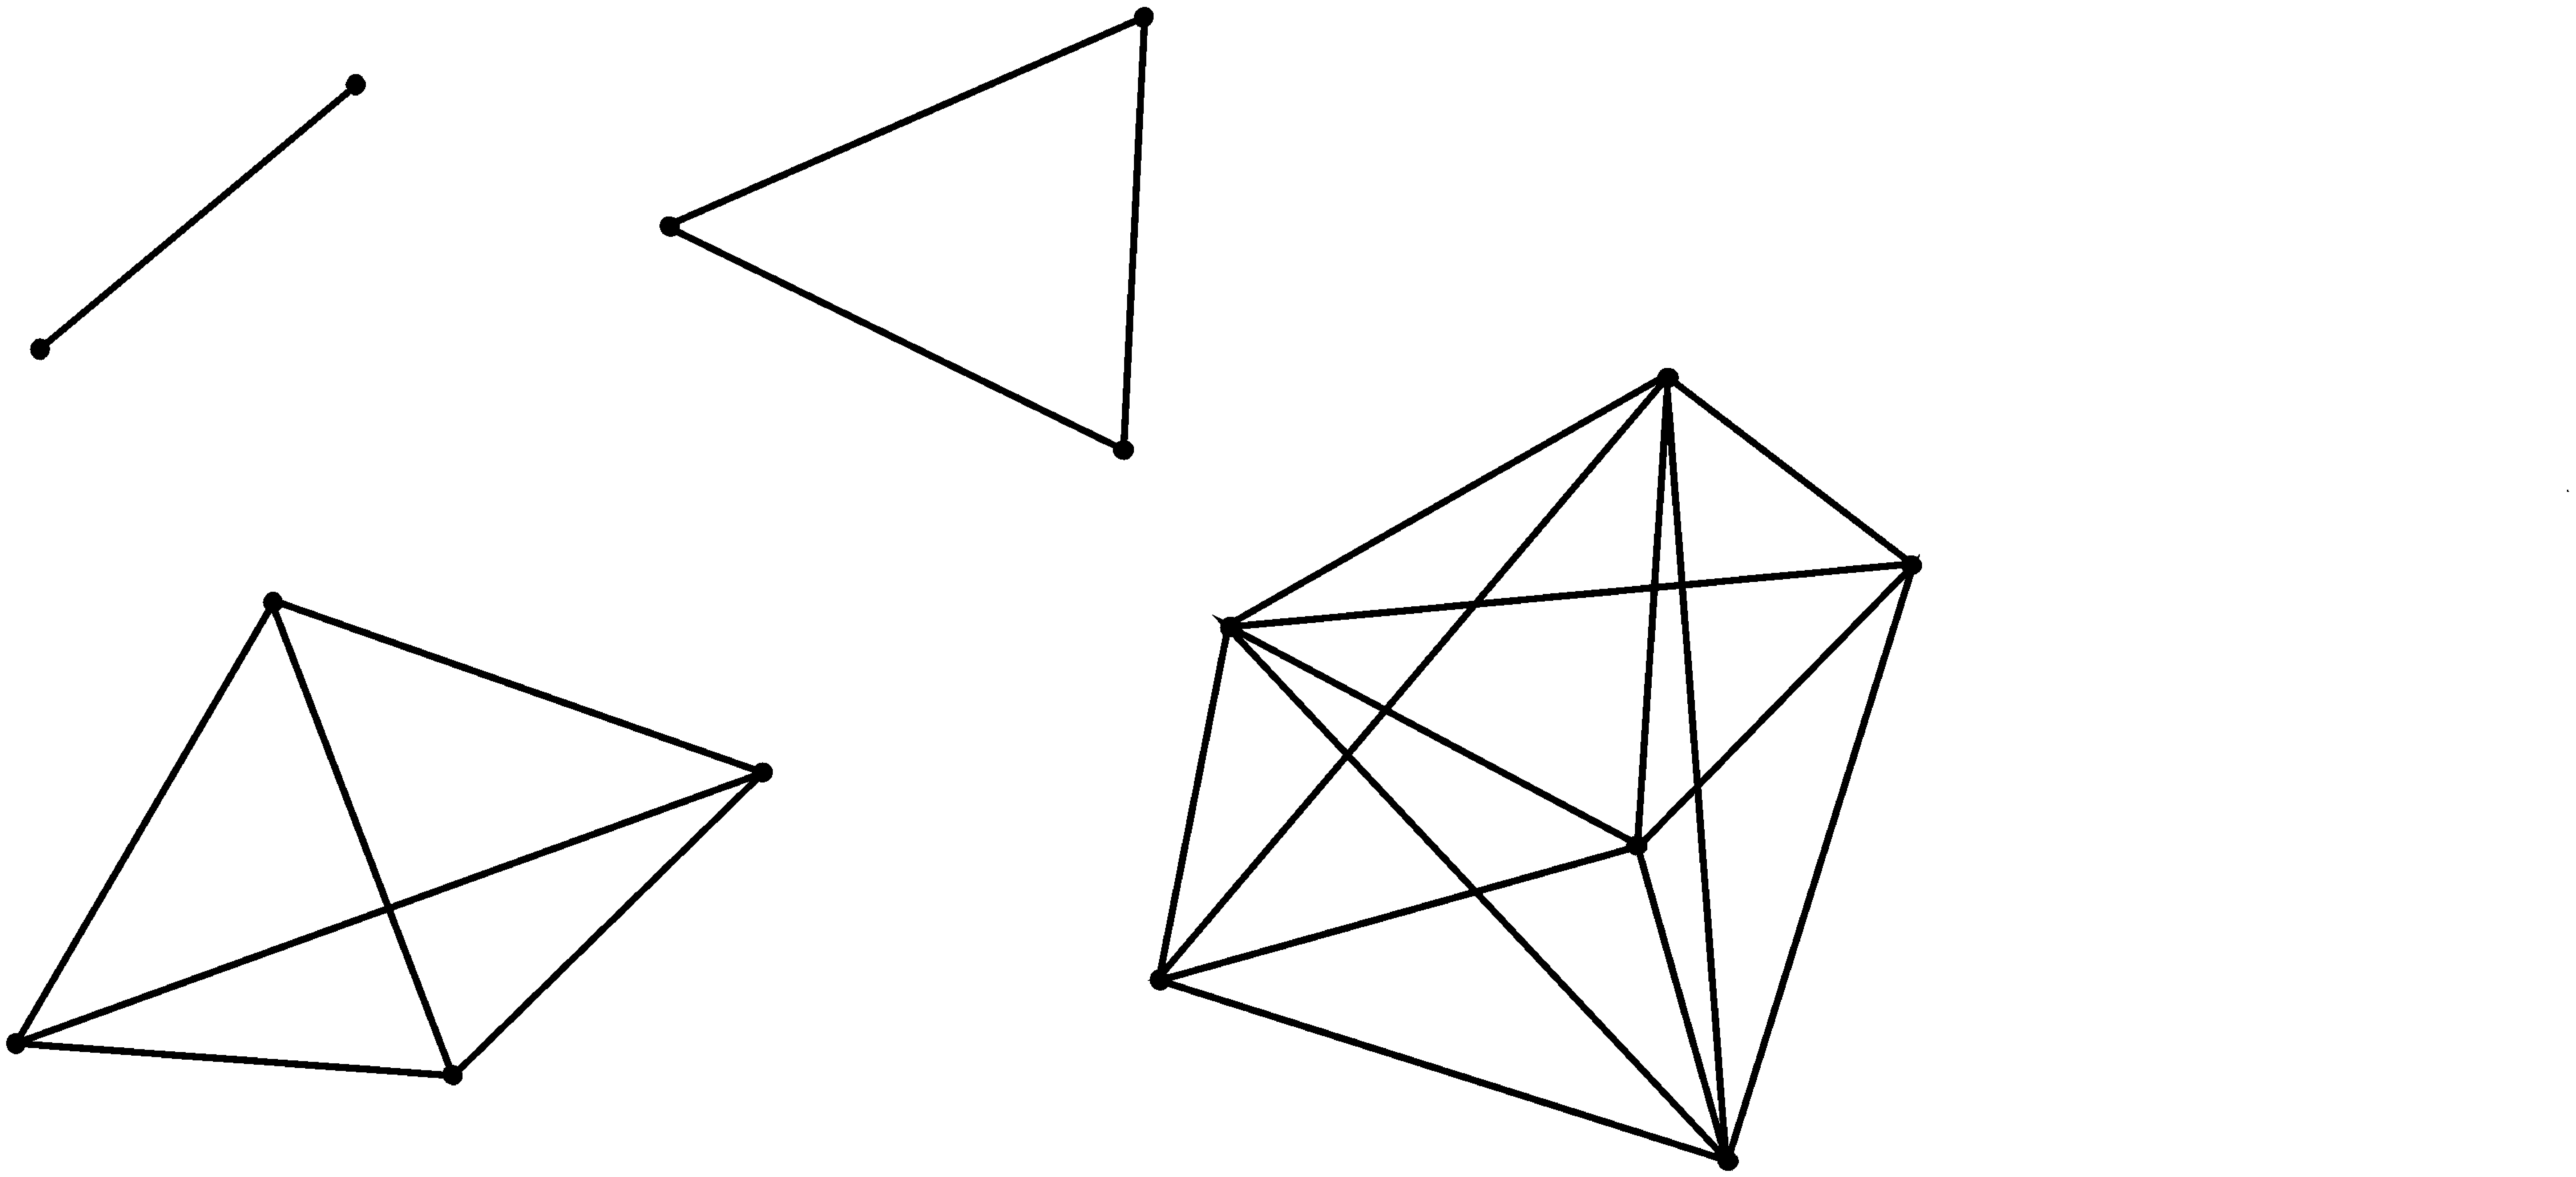
\includegraphics[width=0.6\textwidth]{pict08-2.eps}
\end{center}
 \bigskip
 \refstepcounter{ris}\label{r8-2}

 \centerline{���.~\theris}
 \bigskip
\end{figure}

 \vspace{5mm}

����뢠����,
 $$
 \bigcup_{M_n\subset M} \conv M_n=\conv M.
 $$
 ����⢨⥫쭮, ����� $x,y$ �ਭ�������
 $ \bigcup\limits_{M_n\subset M} \conv M_n,$
 ⮣�� $x$ �ਭ������� �����஬� ᨬ������ $\conv M_n,$
 � $y$ �ਭ������� �����஬� ᨬ������ $\conv M_m.$
 �������⥫쭮, $x$ � $y$ �ਭ������� {ᨬ������} $\conv M',$ ��� $M'=M_n
 \bigcup M_m$ � $[x,y]\subset \conv M' \subset
 \bigcup\limits_{M_n\subset M} \conv M_n.$ ����� ��ࠧ��, $\bigcup
 \conv M_n$ ��㪫�. {�᭮, �� �� ������⢮} �ਭ������� ��� ��㪫��� �������� $V,$
 ᮤ�ঠ饬� $M,$ � ���� �� ����祭��.

 \begin{Corollary} %%% �����⢨�.
 {������⢮}
 $$
 \bigcup_{M_n\subset M} \conv M_n
 $$
 ���� �������襥 ��㪫�� ������⢮, ᮤ�ঠ饥 $M.$
 \end{Corollary}

 \begin{Remark} %%% ����砭��.
 �᫨ $x_1,\ldots, x_n\subset M,$ � $\conv M_n$ {ᮢ������ � ������⢮�}
 $$
 \left\{x=\sum\limits_{k=1}^n c_kx_k:\quad c_k\ge 0,\quad \sum\limits_{k=1}^n
 c_k=1\right\}.
 $$
 \end{Remark}

�뢠�� �㦭� ⠪�� {\it �������� ��㪫�� �����窠} $\overline{\conv M}$
������⢠ $M.$

\ \

\section{��ࠪ���⨪� �������� ��ନ஢����� ����࠭��}

{\bf 1.~����ࠡ��쭮���}
\vspace{3mm}

��ࠪ���⨪�� ���ᨢ���� ����࠭�⢠ ����
 ��������� ��魮��� ���� ���⭮�� ������⢠.

 ����࠭�⢮, ��� ���ண� ������� ����
 ���⭮� ��⭮� ������⢮, ���뢠���� {\it ᥯�ࠡ����}.

 ����࠭�⢮, �� ᮢ�����饥 � $\theta$ � � ���஬ ��� ����
 ���⭮�� ��⭮�� ������⢠, ���뢠���� {\it ��᥯�ࠡ����}.

 ��ࢮ�, �� �� ������ �஢����� ��� ����࠭�⢠ -- ᥯�ࠡ��쭮���.

\vspace{5mm}
{\bf 2.~������}
\vspace{5mm}

����࠭�⢮ ���뢠���� {\it �����}, �᫨ ��猪� ��᫥����⥫쭮���
 ��� (�㭤����⠫쭠� ��᫥����⥫쭮���) ���� �室�饩�� �
 ������-���� �������� ����࠭�⢠.

 ������ �������� ��ନ஢����� ����࠭�⢮
 ���뢠���� {\it ����客� ����࠭�⢮�} ��� ����࠭�⢮�
 ⨯� $B.$

\vspace{5mm}
{\bf 3.~��䫥�ᨢ�����}
\vspace{5mm}

����� $X$ -- ����客� ����࠭�⢮; $X^*$ -- ᮯ�殮���� � ���
 ����࠭�⢮ �������� �����뢭�� �㭪樮�����, �ᥣ�� ����客�; $X^{**}$ -- ��஥
 ᮯ�殮���� ����࠭�⢮.

 ������� �������᪮� �������� $X$ � $X^{**}$ ���।�⢮� ����:
 {��� ���} {$x\in X$ �������}
 $$
 F_{{x}}(f)=f(x),\qquad f\in X^*,
 $$
 ⠪ ��
 $$
 \forall\ x\in X\qquad x\longmapsto F_{{x}}\in X^{**}.
 $$

 ����࠭�⢮ ���뢠���� {\it �䫥�ᨢ��}, �᫨ ��
 �������᪮� �������� $X$ � $X^{**}$ �� ᠬ�� ���� ����� $X\equiv X^{**}$,
 {�.\,�. �� �㭪樮���}
 {$F\in X^{**}$ ᮢ������ � ������� �㭪樮�����}
 {$F_x$ ��� $X^*$.}

 �᫨ ����࠭�⢮ �䫥�ᨢ��, � $X$ � $X^{**}$ ���஥�� ��������� (�������� � ���������).
 ���⭮ ����୮, $X$ � $X^{**}$ ����� ����, ���ਬ��, ��������, ��
 $X$ �� �䫥�ᨢ��.

 �����⭮, �� �᫨  ����࠭�⢮ �䫥�ᨢ��,
 � �� �� ��࠭�祭��� ��᫥����⥫쭮��
 ��� ������⮢ ����� ����� ᫠�� �室������ �����᫥����⥫쭮���.

\vspace{5mm}
 {\bf 4.~��஥��� ���� (��)}
 \vspace{5mm}

 {\bf \normalsize   a) ��ண�� ��㪫����.} ����࠭�⢮ ���뢠���� {\it ��ண� ��㪫�},
 �᫨ ��� ������� �� ��ண� ��㪫�.

 ������� �� ��ண� ��㪫�, �᫨ ��� ���� $x\ne y,$ �ਭ�������� ���, �� �窠
 �� ���ࢠ�� $(x,y)$
 ����� ��ண� ����� ��.

 \begin{Example} %%% �ਬ��.
 ��� -- ��ண� ��㪫�� ������⢮ (��.~8.3), ������ -- �� ��ண�
 ��㪫��. �᭮, �� �᫨ ����࠭�⢮ �� ��ண� ��㪫��,
 � ������� ����௫�᪮���, ����� ��ᠥ��� �����筮��
 �� �����, 祬 � ����� �窥.

 \vspace{0.5cm}
 %%%%%%%%%%%%%%%%%%%%%%%%%%%%%%%%%%%%%%%%%%%%%%%%%%%%%%
 %\hbox to 0.5cm {}{\special{em:graph pict1.pcx}}
 %\vspace{6cm}
 %%%%%%%%%%%%%%%%%%%%%%%%%%%%%%%%%%%%%%%%%%%%%%%%%%%%%%%%%%
 \begin{figure}[ht]
\begin{center}
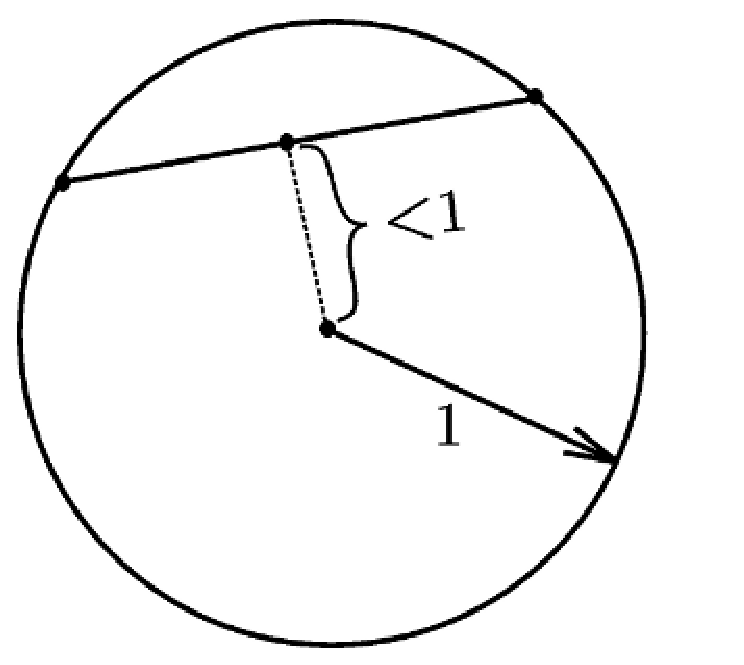
\includegraphics[width=0.3\textwidth]{pict08-3.eps}
\end{center}
 \bigskip
 \refstepcounter{ris}\label{r8-3}

 \centerline{���.~\theris}
 \bigskip
\end{figure}
 \end{Example}

 {\bf \normalsize b) ����६���� �窨} {(�� �������� ����⨥).}
 ����� ������⢮ $M\subset X,~ x\in M.$

 ��窠 $x\in M$ ���뢠���� {\it ������६��쭮�} �窮� ������⢠ $M,$
 �᫨ �������� �窨 $a,b\in M$ ⠪��, �� $x\in (a,b)$
 (��.~8.4). � ��⨢��� ��砥 �窠 ���뢠���� {\it ����६��쭮�}.

%\newpage

 %\vspace{2cm}
 %%%%%%%%%%%%%%%%%%%%%%%%%%%%%%%%%%%%%%%%%%%%%%%%%%%%%%
 %\hbox to 0.5cm {}{\special{em:graph pict1.pcx}}
 %\vspace{6cm}
 %%%%%%%%%%%%%%%%%%%%%%%%%%%%%%%%%%%%%%%%%%%%%%%%%%%%%%%%%%
   \vspace{10mm}
\begin{figure}[ht]
\begin{center}
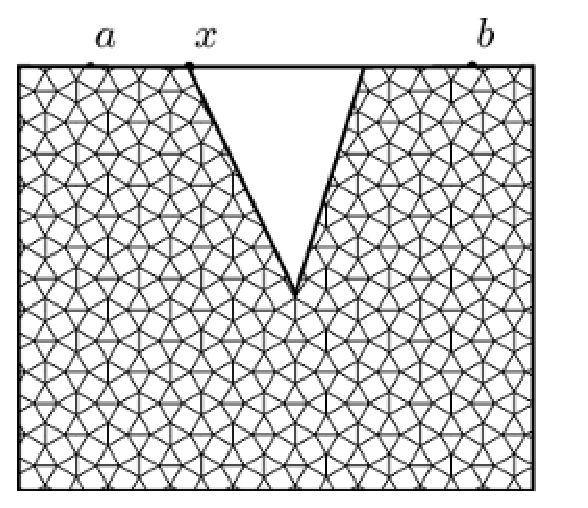
\includegraphics[width=0.3\textwidth]{pict08-4.eps}
\end{center}
 \bigskip
 \refstepcounter{ris}\label{r8-4}

 \centerline{���.~\theris}
 \bigskip
\end{figure}

\vspace{5mm}



 ����� $O_1$ -- ������� ��, $S_1$ -- ���, ��� �࠭��.

 {����� ����}
 \begin{teo}
 � �� ����筮��୮� ����客�� ����࠭�⢥ �� $O_1$ ����
 �������� ��㪫�� �����窠 ᢮�� ����६����� �祪.
 \end{teo}

 ���६� �ਢ���� ��� ������⥫��⢠. � ��饬 ��砥 ��� ����ୠ. �������� ����客�
 ����࠭�⢠, � ������ ������� �� �� �����
 ����६����� �祪.

 \ex
 ��������, �� � �����筮� �� $O_1$  � $L{[0,1]}$ ��� ��
 �����  ����६��쭮� �窨.

 \ex
 ��������, �� �� $O_1$ � $C[0,1]$ ����� ��� ����६����� �窨.

\vspace{5mm}
 {\bf \normalsize c) ���������.}
 ����࠭�⢮ ���뢠���� {\it �������}, �᫨ ��� ��
 �窨 �� $S_1$ ������� �����⢥��� ����� �㭪樮���,
 �.\,�. �����⢥���� ���⥫쭠� ����௫�᪮��.
 ��।������ ���⥫쭮� ����௫�᪮�� �㤥� ���� �����.

 � ��⨢��� ��砥 ����࠭�⢮ �� ������.

\vspace{5mm}
 {\bf 5.~�������� ������⢠}
 \vspace{5mm}

  ������⭮� ������⢮ -- ⠪�� ������⢮, �� ��
 ��᫥����⥫쭮��
 ���ண� ����� ����� �室������ �����᫥����⥫쭮��� � �������� �⮣� ������⢠.

 ������⭮� ������⢮ �ᥣ�� �������.

 \vspace{3mm}
 \section{�᭮��� ����࠭�⢠}
  \vspace{3mm}

 {\it ����࠭�⢮ $C=C(Q,X)$ -- �� ����࠭�⢮ �����뢭�� �㭪権}, ��।�������
 �� ������� $Q$ � �ਭ������ ���祭�� �� ����客� ����࠭�⢠ $X.$
 ������᪨� ��砨: $X=\bR,$  $\ X=\bC.$
 \vspace{3mm}

 1. {����࠭�⢮ $C(Q,X)$} ������.
 \vspace{3mm}

 2. �� �������� $Q$ � $X$ ����࠭�⢮ {$C(Q,X)$} ᥯�ࠡ��쭮, � �� �������� -- ���.

 �᫨ $Q$ -- ��१��, $X=\bR,$ � $C(Q,X)$ ᥯�ࠡ��쭮.
  \vspace{3mm}

 3. �᫨ $Q$ ��᪮��筮, � $C$ ���䫥�ᨢ��; � ��⭮��, $C[0,1]$ ���䫥�ᨢ��.
  \vspace{3mm}

 4. {�� ���� $Q,$ $X$ ����࠭�⢮ $C(Q,X)$} �� ��ண� ��㪫�� ����࠭�⢮ {� ��} {�������.}
\vspace{3mm}

 \ex %%%��ࠦ�����.
{�������� �� ᢮��⢠.}

{{\it ����࠭�⢮} $ L^{{p}},~ 1\le p< \infty.$}

 ����� ������ ����࠭�⢮ $Q$ � ��ன $\mu$ ($\mu$ --
 ��⭮ ����⨢��� ������⥫쭠� �㭪�� ����ਬ�� ���������� �� $Q$).

 ����� $y=f(x)$ -- ��।������� �� $Q$ ����ਬ��
 �㭪�� {� ���祭�ﬨ � $\bR$ ��� $\bC$,} ��� ���ன
 ��⥣ࠫ  $\ds\int_Q |f(x)|\ d\mu$ ����祭, $L_{{\mu}}$ -- ������⢮ ⠪�� �㭪権 �
 $\ds\int_Q |f(x)|\ d\mu=\pnl f\pnr$ -- ���㭮ଠ.
 ��� ⮣�, �⮡� ������� ����客� ����࠭�⢮, 䠪�ਧ㥬 $L_{{\mu}}$:
 $$
  \left. L_{{\mu}} \right/ \{f:\ \pnl f\pnr =0{\}},
  $$
 {�.\,�. �㤥� �⮦���⢫��� �㭪樨, ࠧ����騥�� ���� �� ���������⢥ �㫥���} {����.}
 ����稬 ������ ����࠭�⢮, ���஥ � ����� �㤥� ��������� $L_{{\mu}}.$

 ����ࠡ��쭮��� $L_{{\mu}}$ ������ �� $Q$ � �� $\mu;$ �᫨ $\mu$ --
 ��� ������ �� $Q\subset\bR^n,$ � $L_{\mu}=L_{\mu}^1(Q)=L(Q)$ ᥯�ࠡ��쭮.

 �⮡� ������� $L^p_\mu$, ���쬥� ���㭮��
 $$
 \pnl f \pnr =\left( \int_Q |f(x)|^p\, d\mu \right)^{1/p}.
 $$
{ ����� ���������⭮��, ᮮ⢥�����騩 �㭪樨 $f$, �㤥� ��������� ⥬ ��}
{ᨬ����� $f$ � ��⮬� $\pnr f\pnr=\|f\|_{L^p}$ -- ��ଠ.}

 �� $p=2$ ����稬 {$L^2_\mu$} -- ���졥�⮢� ����࠭�⢮ � ᪠����
 �ந���������
 $$
 (f,g)=\ds\int_Q {fg}\ d\mu
 $$
 ��� ����� ����⢨⥫��� �ᥫ,
 $$
 (f,g)=\ds\int_Q {f{\overline g}}\ d\mu
 $$
 ��� ����� ���������� �ᥫ; {$L^2_\mu$}~--
 ������ �⭮�⥫쭮 ���� $\|f\|_{{L^2}}=\sqrt{(f,f)}$ {����࠭�⢮}.

 ��������, �� � ����࠭�⢠� $L^p,\ L^q,$ �� $\dfrac{1}{p}+\dfrac{1}{q}=1,\ 1<p,\ q<\infty$
 ��ࠢ���⢮ �\"{�}�줥�
 $$
 \left| \int_{a}^b f(x)g(x)\,dx\right| \le
 \|f\|_{L^p[a,b]}\|g\|_{L^q[a,b]}
 $$
 ��� $f\in L^p[a,b],\ g\in L^q[a,b]$ �ॢ�頥��� �
 ࠢ���⢮ ⮫쪮 �᫨ $f(x)g(x)\ge 0$ ���� ���� �
 $|f(x)|^p$ ���� ���� �ய��樮����� $|g(x)|^{q}.$

 \begin{ex}
���ᬮ���� ��� ������ ��� �㭪権 �� $L^p_{\mu}(Q)$ � $L^q_{\mu}(Q).$
 \end{ex}

 % ���樨 ��ࣥ� ���ᮢ�� ��窨��
% ??? ���ᥭ� ��ࠢ����� �.�.����襢�
% ���ᥭ� ��ࠢ����� �.�.�����, ����� 23.07.2009
% ���ᥭ� �ࠬ����᪠� � ���-�ࠢ�� �.����������, ����� 05.08.09


%%%%%%%%%%%%%%%%%%%%%%%%%%%%%
\chapter{��騥 ������� ����� ⥮ਨ �ਡ�������}
%%%        ����� 9.

\section{��㪫���� ����࠭�⢠ $L^p$}

�த������ ��ᬠ�ਢ��� ����࠭�⢠ ${L^p},$~ $1\le p<\infty.$ �� $p=2$ ����࠭�⢮
 ${L^2}$ ���졥�⮢�. ����� ��⠥�, �� $\mu$ -- ���
 ������.

����� ���� ᫥�����, �ਢ������ ����� ��� ������⥫��⢠
 \begin{teo}    %%% ���६�.
 ������ ��ନ஢����� ����࠭�⢮ {$H$ ���졥�⮢�} ⮣�� � ⮫쪮 ⮣��, ����� �� ���
 ����筮���� �������࠭�⢠, ������ ���, �᫨ ��� ����筮��୮,
 ���������.
 \end{teo}


 \begin{Corollary} %%% �����⢨�.
 � ���졥�⮢�� ����࠭�⢥ ��ୠ ���᪠� ��������.
 \end{Corollary}

 \begin{Example} %%% �ਬ��.
 ��ࠫ�����ࠬ� �������� ᢮��⢮�:
  �㬬� �����⮢ ���������� ࠢ�� �㬬� �����⮢ ��� ����� ��஭,
  �.\,�.
 $$
 \|x+y\|^2+\|x-y\|^2=2(\|x\|^2+\|y\|^2)
 $$
 (����� ��ࠫ�����ࠬ��). � ���� �������
  �����뢠����, �� 㦥 �� ᢮��⢮ �ࠪ�ਧ�� ���졥�⮢�
  ����࠭�⢮.
 \end{Example}

 �� $p\ne 2,$~ $p>1,$ ����࠭�⢮ ${L^p}$ (�᫨ ��� ࠧ��୮��� ����� 1)
 �� ���� ���졥�⮢�,
 �� ���� ��ண� ��㪫� � �䫥�ᨢ��.

 � �� ����客�� ����࠭�⢥ ��ଠ 㤮���⢮���  ��ࠢ�����
 ��㣮�쭨��
 $$
 \|x+y\|\le \|x\|+\|y\|.
 $$
 � ${L^p}$ ����砥�
 $$
 \left\{ \int_Q {|x+y|}^p\, dt \right\}^{1/p} \le
 \left\{ \int_Q |x|^p\, dt \right\}^{1/p}+
 \left\{ \int_Q |y|^p\, dt \right\}^{1/p}
 $$
 -- ������᪮� ��ࠢ���⢮ ������᪮��. �����
  ࠢ���⢮ (� ����⢥���� ��砥) �㤥� ⮣�� � ⮫쪮 ⮣��, �����
 $x$ � $y$ ������⥫쭮 �ய��樮�����, �.\,�. ��������
 $\alpha,\beta \ge 0$ � $\alpha^2+\beta^2>0$ ⠪��, �� $\alpha
 x=\beta y,$ �.\,�. $x$ � $y$ ����� �� ����� ���, ��室�饬 �� ��砫�
 (�. �᫮��� ��.~9.1).

 �� ᢮��⢮ ���뢠���� ᢮��⢮� {\it ��ண��
  ��ନ஢������}; ��� ���������⭮ ��ண�� ��㪫��� ����࠭�⢠.

  \begin{figure}[ht]
\begin{center}
\includegraphics{pict09-1.eps}
\end{center}
 \bigskip
 \refstepcounter{ris}\label{r9-1}

 \centerline{���.~\theris}
 \bigskip
\end{figure}


 �������⥫쭮, ��� ��� $p>1$ ����࠭�⢮ ${L^p}$ ��ண� ��㪫�. ����࠭�⢮ ${L^1}$
 �� ���� ��ண� ��㪫�; ��� ���᭮����� �⮣� ����ந� � ${L^1}[0,1]$
  ��� ������� $x$ � $y$ ⠪��, �� � ��ࠢ���⢥ ������᪮��
  {�믮������ ࠢ���⢮}, �� $x$ � $y$ �� ���� ������⥫쭮 �ய��樮�����:
  {�����筮 ��������}
  $$
    {
    x(t) = \begin{cases}
      1, & t \in [0,1/2)  \\[7pt]
      0, & t \in [1/2,1]
    \end{cases},\qquad
    y(t) = \begin{cases}
      0, & t \in [0,1/2)  \\[7pt]
      1, & t \in [1/2,1]
    \end{cases}.}
  $$

 % \vspace{1cm}
 %%%%%%%%%%%%%%%%%%%%%%%%%%%%%%%%%%%%%%%%%%%%%%%%%%%%%%
 %\hbox to 0.5cm {}{\special{em:graph pict1.pcx}}
 %\vspace{6cm}
 %%%%%%%%%%%%%%%%%%%%%%%%%%%%%%%%%%%%%%%%%%%%%%%%%%%%%
 �� ��.~\ref{r9-2} �।�⠢��� �� ���� ��ਠ�� �㭪権
 $x$ � $y.$

 \bigskip
\begin{figure}[ht]
\begin{center}
\includegraphics{pict09-2.eps}
\end{center}
 \bigskip
 \refstepcounter{ris}\label{r9-2}

 \centerline{���.~\theris}
 \bigskip
\end{figure}

 �ਬ�� ����� �����࠭��� �� ����࠭�⢠ $L_{\mu}.$

 %\bigskip

 \section{�������ୠ� ��㪫����}

 ���쬥� ������� �� $O_1$ � ����客�� ����࠭�⢥, �஢���� ����௫�᪮���
  �� ����ﭨ� $h<1$ �� $\Theta_X,$ <<��०�� ���⨪>> $l$ �� �� $O_1$ (�. ��.~\ref{r9-3}).
   �㤥� ���� $d(l)$
  -- ������� <<���⨪�>>. ������ ���६�� $h$ � $1$ � ��ᬮ�ਬ
 $\lim\limits_{h\to 1} d(l).$

 \bigskip
\begin{figure}[ht]
\begin{center}
\includegraphics{pict09-3.eps}
\end{center}
 \bigskip
 \refstepcounter{ris}\label{r9-3}

 \centerline{���.~\theris}
 \bigskip
\end{figure}


\noindent � ���������� ����࠭�⢥ $d(l)\to 0$~ $(h\to 1).$

 ����࠭�⢮ ���뢠���� {\it ࠢ����୮ ��㪫�}, �᫨
  ������� $d(l) \rightrightarrows 0$~ $(h\to 1)$
  ࠢ����୮ �� �ᥬ ����௫�᪮��� {(�� �ᥬ <<���⨪��>>)}.
  �᭮, �� ࠢ����୮ ��㪫�� ����࠭�⢮ -- ��ண�
  ��㪫��.

 {����� ����} ᫥����� ⥮६�, ������ ⠪�� �ਢ����
 ��� ������⥫��⢠.
 \begin{teo}[����ᮭ] %%% ���६�
 ��类� ࠢ����୮ ��㪫�� ����客� ����࠭�⢮ �䫥�ᨢ��.
 \end{teo}

 �������� ࠢ������� ��㪫���� ����࠭�⢠ ${L^p}$ �� $p>1,$
 ����, ᫥����⥫쭮, ${L^p},$~ $p>1$,  �䫥�ᨢ��. ${L^1},$
 ����� ������, �� �䫥�ᨢ��, �� �᪫�祭���
 ��஦������ ��砥�, ����� ��� ��।��祭� �
 ����筮� �᫥ �祪.

 \section{��騥 ������� ����� ⥮ਨ �ਡ�������}

 {\bf ���⠭���� �����.} ����� $X$ -- ����客� ����࠭�⢮,
 $L$ -- ᮡ�⢥���� �������࠭�⢮ $(L\ne X)$ ($L$ �������).

 ���ᬮ�ਬ ������ � ������襬 �ਡ�������
 ��� ������� $x\in X$ �� ����� ������⮢ $y\in L,$ �.\,�. ��ᬮ�ਬ
 ������
 $$
 \inf_{y\in L} \|x-y\|_X=E(x,L)_X.
 $$

 \vspace{3mm}
 {\bf 1.~�஡���� �����⢥�����}
 \vspace{3mm}

 ��� ��� $x\in X$ ��⠢�� ������⢮ $Y(x)$
 (����� ����, � ���⮥):
 $$
 Y(x)=\{ y^*\in L : \|x-y^*\|_X=E(x,L)_X\}
 $$
 -- ������⢮ (��� ������࠭���) �������� ������⮢;
 $$
 x\longmapsto Y(x)\subset L.
 $$

����� ��᫥����� ᫥�����

 \task %%% �����.
 �� ����� �᫮���� �� $X$ ��� ��� $x\in X$ � ��� $L$
 ��魮��� $\mbox{card}\ Y(x)\le 1?$ �.\,�. ��� ����� $X$
 ��� ��� $x\in X$ � �� �������࠭�⢥ $L$
 ������� �� ����� ������ ������襣� �������?

\begin{defi}
 �᫨ ��� ��� �������࠭�⢠ $L$ � ��� ��� ������� $x\in X$
 �������� ⮫쪮 ���� ��� {�� ��������} �� ������ ������襣� �������, � �㤥�
 �������, �� $X$ �������� {\it ᢮��⢮� �����⢥�����} $(U).$
 \end{defi}

 \begin{teo} %% ���६�.
 ��� ⮣� �⮡� ����客� ����࠭�⢮ �������� ᢮��⢮� $(U)$,
 ����室��� � �����筮, �⮡� ��� �뫮 ��ண� ��㪫�.
 \end{teo}

 \begin{proof} %%% ������⥫��⢮.
 �\;�\;�\;�\;�\;�\;�\;�\;�\;�\;�\;�\;�.~ ����� $X$ ��ண� ��㪫�. �।�������, ��
 $(U)$ �� �믮������, �.\,�. �������� $L\subset X,$ $x\in
 X$ � $y_1,y_2$ ⠪��, ��
 $$
 \{y_1,y_2\}\subset Y_L(x),\qquad y_1\ne y_2.
 $$
 �����
 $$
 \inf_{y\in L} \|x-y\|=\|x-y_1\|=\|x-y_2\|=E(x,L)_X>0.
 $$
 ���ᬮ�ਬ ������� $y=\dfrac{1}{2}(y_1+y_2).$ �����⠥� 㪫������ $x$
 �� $y$:
 $$
 \|x-y\|=\left\| \frac{1}{2} (x-y_1)+\frac{1}{2}(x-y_2) \right\|.
 $$
 ������� $x-y$ ���� �।��� ��१�� $[x-y_1,x-y_2],$ �����
 ���ண� ����� �� ��� $S$ ࠤ��� $\rho=E(x,L)_X.$
 ����� � ᨫ� ��ண�� ��㪫��� ����࠭�⢠ ������� $x-y$
 ����� ��ண� ����� �� ${O}_{\rho},$ �����, ����� ��ண� ������� ����, �.\,�.
 $$
 E(x,L)_X \le \|x-y\|=\left\| \frac{1}{2}(x-y_1)+\frac{1}{2}(x-y_2)
 \right\|<\|x-y_1\|=\|x-y_2\|=E(x,L)_X
 $$
 -- ��⨢��稥.



 {�\;�\;�\;�\;�\;�\;�\;�\;�\;�\;�\;�\;�.}~ ����� $X$ �������� ᢮��⢮� $(U),$
 ���� ��������, �� ⮣�� $X$ ��ண� ��㪫�. �।�������, �� $X$
 �� ��ண� ��㪫�, ⮣�� ������� ����௫�᪮��� $L,$
 ����ﭨ� �� ���ன �� {��砫�} $\theta_X$ ࠢ�� 1 � �����
 ��ᠥ��� �����筮� ���� �� �ࠩ��� ��� � ���� �窠� $s_1,s_2.$
 <<�������>> ����௫�᪮��� ⠪, �⮡� $L\to L_1,$~ $\theta_X\to x_0,$~ $L_1$
 -- �������࠭�⢮, �.\,�. $L_1\ni \theta_X,$ ⮣�� $s_1\to y_1,$~ $s_2\to y_2.$

 \bigskip
\begin{figure}[ht]
\begin{center}
\includegraphics{pict09-4.eps}
\end{center}
 \bigskip
 \refstepcounter{ris}\label{r9-4}

 \centerline{���.~\theris}
 \bigskip
\end{figure}


 ���ᬮ�ਬ ������� $x_0$ (�. ��.~\ref{r9-4}). ��� ���� � �������࠭�⢥ $L_1$
 ���� �� �ࠩ��� ��� ��� ������� ������襣�  �ਡ������� $y_1$
 � $y_2.$ ��⨢��稥. ���६� ��������.
 \end{proof}

\begin{Remark} %%% ����砭��.
  { �� 䠪��᪨ ��������, �� �᫨ $y_1\in Y(x),$~ $y_2\in Y(x),$
 �.\,�.
 $$
 E(x,L)=\|x-y_1\|=\|x-y_2\|,
 $$
 � $[y_1,y_2]\subset Y(x).$}
 \end{Remark}

{ ����⢨⥫쭮, �� ������� $y$ �� $[y_1,y_2]$
 �।�⠢����� � ���� $y=ty_1+(1-t)y_2$ �� �����஬ $t\in [0,1].$
 �����
 $$
{E(x,L)\le} \|x-y\|=\|t(x-y_1)+(1-t)(x-y_2)\|\le t\|x-y_1\|+(1-t)\|x-y_2\|=E(x,L).
 $$}

  \begin{Corollary} %%% �����⢨�.
 ������࠭��� �������� �ਡ������� -- �ᥣ�� ��㪫�� ������⢮ $($�, �����, ���
 ��ண� ��㪫��� ����࠭�⢠ �� ���� ����, ���� ��⮨�
 ⮫쪮 �� ������ �������$)$.
 \end{Corollary}

 �� ������᪨� ����࠭�� ����࠭�⢠ $C$ � ${L^1}$ �� ����� ��ண� ��㪫묨,
 ᫥����⥫쭮, $C$ � ${L^1}$ �� �������� ᢮��⢮� �����⢥�����.
 {����࠭�⢠} ${L^p},$~ $p>1,$ ��ண� ��㪫�, ᫥����⥫쭮, �������� ᢮��⢮�
 �����⢥�����.

 � ��饬 ��砥 �� �������࠭�⢠ $\{L\}$ ����࠭�⢠ $X$
 ������� �� �������騥 �  �� �������騥 ᢮��⢮� �����⢥�����.
 {�� {��.~\ref{r9-5}} ����ࠦ��� ��� � ���}
 {�������࠭�⢠ ����࠭�⢠ �� ���᪮�� � ��ମ�,
 ��।��塞�� �⮩ ��ன.

 \begin{figure}[ht]
\begin{center}
\includegraphics{pict09-5.eps}
\end{center}
 \bigskip
 \refstepcounter{ris}\label{r9-5}

 \centerline{���.~\theris}
 \bigskip
\end{figure}


 \vspace{3mm}
 {\bf 2.~�஡���� ����⢮�����}
  \vspace{3mm}

 �᫨ ���  ��� $x\in X$ � �� �������࠭�⢥ $L$
 ��������  ��� �� ���� ������訩 �������, � �㤥� �������, �� $X$
 �������� ᢮��⢮� ����⢮����� $(E).$

�㤥� �������, �� ����௫�᪮��� {$L_1$} ��ᠥ��� ����
$S_1$, �᫨ ������� ������� $y\in S_1=\{ z\in X:\ \|z\|=1\}$
⠪��, �� $\inf\limits_{x\in {L_1}} \|x-y\|=0.$ ����⨬, �� ��ᠭ�� �� �।�������� ����稥 �窨 ��ᠭ��.

��� ����客�� ����࠭�� {����� ����}
 \begin{teo}[������] %%% ���६�
 ��� ⮣� �⮡� ����客� ����࠭�⢮ �뫮 �䫥�ᨢ��, ����室��� �
 �����筮, �⮡� ��猪� ����௫�᪮��� �⮣� ����࠭�⢠,
 �������� �����筮� ����, ����� $($��� �� ����$)$ ��� ��ᠭ��
 {���, �� � �� ᠬ��, ��猪� ����௫�᪮��� $L_x=\{y : f(y)=f(x)\}$ ����� �� ���}
 {��ᠭ�� � ��ன $S_E=\{z\,:\,\|z\|=E(x,L)\},$ ��� $L$~-- ������⠭�⢮ $\{y:f(y)=0\}.$}
 \end{teo}

% \begin{proof} %%% ������⥫��⢮.
 ����� ��ࠧ��, ����࠭�⢮ $X$
  �䫥�ᨢ�� ⮣�� � ⮫쪮 ⮣��, ����� ��� ��� $f\in X^*$
 �������� $x\in X$ ⠪��, �� $\|x\|=1$ � $|f(x)|=\|f\|$
 (�.\,�. �� ������� $x$ ���⨣����� ��ଠ �㭪樮����).
 %�� ��࠭�稢�� ��魮��,
 %����� �����, �� $\|f\|=1.$ ����� ������⢮ $\{ y : f(y)=1\}$
 %-- ����௫�᪮��� � ������ ����⢮���� ������� $x,$~ $\|x\|=1$,
 %⠪��, �� $f(x)=1.$
 %\end{proof}

 \begin{Example} %%% �ਬ��.
 � $C[0,1]$ ��ᬮ�ਬ �㭪樮��� $f(x)=\ds\int_0^1 \sign\sin 2\pi t\cdot
 x(t)\,dt.$ ��ଠ �⮣� �㭪樮����
 $$
 \|f\|=\int_0^1 |\sign\sin 2\pi t|\, dt=1,
 $$
 �� ��� �� ���⨣����� � $C,$ ⠪ ��� �㭪�� $x(t)=\mbox{sign} \sin
 2\pi t$ �� �ਭ������� $C[0,1].$


 \noindent � �⮬ �ਬ�� �窨 ��ᠭ�� ����௫�᪮�� $f(x)=1$ � �����筮� ��ன
 $S_1$ � $C[0,1]$ ��� (��� ����� ������, ��� �� $x(t)\in C[0,1],~ \|x\|_C=1,~
 \Longrightarrow |f(x)|<1$).
 \end{Example}

 \begin{teo} %%% ���६�.
 ����客� ����࠭�⢮ �������� ᢮��⢮� $(E)$
 � ⮬ � ⮫쪮 ⮬ ��砥, ����� ��� �䫥�ᨢ��.
 \end{teo}

 \begin{proof} %%%������⥫��⢮.
 1) ����� $X$ �� �䫥�ᨢ��. ����� �� ⥮६� ������ �������
 ����௫�᪮��� $\{ f(x)=1\},$ {$\|f\|=1,$} ����� �� ����� �窨 ��ᠭ�� �
 �����筮� ��ன. ���ᬮ�ਬ �������࠭�⢮ $L=\{{y}:f(y)=0\}.$
 ����� ��� ��� ������� $x$ ⠪���, �� $f(x)\ne 0$ � $L$
 ��� ������襣� ������� (�᫨ �� ��, � ��᫥
 <<ᤢ���>> ����稫� �� ��� ��ᠭ�� ��� ����௫�᪮�� $L_x$ {(�. ��.~9.6)}).

 \vspace{10mm}
 %%%%%%%%%%%%%%%%%%%%%%%%%%%%%%%%%%%%%%%%%%%%%%%%%%%%%%
 %\hbox to 0.5cm {}{\special{em:graph pict1.pcx}}
 %\vspace{6cm}
 %%%%%%%%%%%%%%%%%%%%%%%%%%%%%%%%%%%%%%%%%%%%%%%%%%%%%%%%%%
 %\noindent \hskip3.0cm {��.}
 %\bigskip
\begin{figure}[ht]
\begin{center}
\includegraphics{pict09-6.eps}
\end{center}
 %\bigskip
 \refstepcounter{ris}\label{r9-6}

 \centerline{���.~\theris}
% \bigskip
\end{figure}

 2) ����� $X$ �䫥�ᨢ��. �������, �� ⮣�� ��� �������� ᢮��⢮�
 $(E).$ �०�� �ᥣ� ����⨬, �� �᫨ $\{ x_n\}\in L$ � $x_n \dashrightarrow x$
 (᫠�� �室���� � $x$), � $x\in L$ �
 $$
 \|x\|\le d =
 \mathrel{\mathop{\underline{\lim}}\limits_{n\to \infty}} \|x_n\|.
 $$

 ����� ⥯��� $L$ -- �� �������࠭�⢮ � $x$ -- �� ������� ��
 $X,$ {$x\not \in L.$} ����ந� ��� $O_{d+\varepsilon_n}=O_{d+\varepsilon_n}(x)$ (�. ��.~9.7) � 業�஬ � $x$
 � ࠤ��ᮬ $d+\varepsilon_n,$ ��� $d=E(x,L)$ � $\varepsilon_n
 \downarrow 0.$ ���ᬮ�ਬ ������⢠ $K_n=O_{d+\varepsilon_n}\cap L.$
 $\{K_n\}$ -- ��������� ��᫥����⥫쭮��� �������� ��࠭�祭���
 ��������� �������.  � �䫥�ᨢ��� ����࠭�⢥ ⠪�� ��᫥����⥫쭮���
 ����� �����⮥ ����祭��. ����⢨⥫쭮, ���쬥�
 $$
 x_n\in K_n,\qquad \|x-x_n\| \longrightarrow d.
 $$
 ��᫥����⥫쭮��� $\{x-x_n\}$~-- ᫠�� ������⭠�. �����⭮, �� �� ��� �����
 ����� �����᫥����⥫쭮��� $\{x-x_{n_k}\},$
 ᫠�� �室������ � �����஬� �������� $x-x_0,\ x_0\in \cap K_n.$ �������⥫쭮,
 $x_0\in L$ � $\|x-x_0\|\le
 d.$ ��� ��� $d=E(x,L),$ � ��ண��� ��ࠢ���⢠ �� ����� ����, ⠪ ��, �� ᠬ�� ����
 $\|x-x_0\|=d$ �, �����, $x_0$ -- ������訩 �������. ���६� ��������.
 \end{proof}

 \bigskip
\begin{figure}[ht]
\begin{center}
\includegraphics{pict09-7.eps}
\end{center}
 \bigskip
 \refstepcounter{ris}\label{r9-7}

 \centerline{���.~\theris}
 \end{figure}



 \begin{Corollary} %%% �����⢨�.
 ��类� ����筮��୮� �������࠭�⢮ ���� ������⢮ ����⢮�����.
 \end{Corollary}

 \begin{Remark} %%% ����砭��.
 ��类� ��࠭�祭�� ������⭮�
 ������⢮, �.\,�. ������⢮, ����祭�� ���ண� � ���
 �஬ $O_d(x)$ ������⭮, ���� ������⢮ ����⢮�����.
 \end{Remark}

 \begin{Example} %%% �ਬ��
 {(����筮-��ࠬ����᪮�� ������⢠} �� ��饣��� ��࠭�祭�� ��������).
 � $C[0,1]$ ��ᬮ�ਬ ������⢮ �樮������ �஡�� ���� $R_1=\dfrac{a}{b+ct}\in C[0,1].$
 $R_1$ ������ �� ��� ��ࠬ��஢ $a,b,c;$ �� ������⢮ �� ������⭮ � $C[0,1]$:
 ��᫥����⥫쭮��� $\left\{ \dfrac{1}{1+ct}\right\}$
 {�� $c \to 0$}
 �室���� �� $(0,1]$
 � $0,$ � � �窥 {$t=0$} �ਭ����� ���祭��, ࠢ��� $1.$

 ����࠭�⢮ ${L^p},~ p>1,$ ���� � �䫥�ᨢ��, � ��ண� ��㪫�,
 ᫥����⥫쭮, � $L_p,~ p>1,$ �� �������࠭�⢮ ���� �
 �������࠭�⢮ $(U)$, � �������࠭�⢮~$(E).$

 ����� �������࠭�⢠, ��騥�� �
 �������࠭�⢠�� �����⢥�����, � ������⢠��
 ����⢮�����, ���뢠���� {\it 祡�襢᪨��}
 �������࠭�⢠��.
 \end{Example}

 % ���樨 ��ࣥ� ���ᮢ�� ��窨��
% ??? ���ᥭ� ��ࠢ����� �.�.����襢�
% ���ᥭ� ��ࠢ����� �.�.�����, ����� 23.07.2009
% ���ᥭ� �ࠬ����᪠� � ���-�ࠢ�� �.����������, ����� 05.08.09

%%%%%%%%%%%%%%%%%%%%%%%%%%%%%
\chapter{���਩ ������襣� \\
 �ਡ������� � $\boldsymbol L^p$. ���४⭮���}
%%% ����� 10.


 \section{���਩ ������襣� ������� � $L^p$}

  %%% ����砭��.
 ����� $H$ -- ���졥�⮢� ����࠭�⢮. � ���� �������
 �����뢠����, �� ��� ⮣� �⮡� $y^*$ �� ������訬 ������⮬ �
 �������࠭�⢥
 $M\subset H$ ��� ������� $x,$ ����室��� � �����筮, �⮡�
 $$
 (x-y^*,y)=0\qquad \forall\  y\in M.
 $$
 �᫨ $H=L_2,$ � �� �᫮��� ����� ��९����
 $$
 \int_Q (x-y^*)y\, dt=0\qquad \forall\  y\in M.
 $$


 ����뢠����, �� �⢥ত���� ���� ����
 ��砩 ����� ��饩 ⥮६�, ����� ���� ����室����
 � �����筮� �᫮��� ��� ������襣� ������� � $L_p,$~ $p>1.$

 \begin{teo} %%% ���६�.
 ����� $p>1,$~ $M\subset L_p$ -- �������࠭�⢮, $ \ x\in L_p.$
 ��� ⮣�, �⮡� $y^*$ �� ������訬 ������⮬ �� $M$ ��� $x$
 � $L_p$ ����室��� � �����筮, �⮡�
 \begin{equation}\label{f9-1}
 {\int_Q |x-y^*|^{p-1} \sign (x-y^*)y\, dt=0} {\qquad \forall\  y\in M}.
 \end{equation}
 \end{teo}

 \begin{proof} %%% ������⥫��⢮.
 �\;�\;�\;�\;�\;�\;�\;�\;�\;�\;�\;�\;�.~ ����� �᫮��� \eqref{f9-1}
 �� �믮������, �.\,�. ������� $y\in M$ ⠪��, ��
 $$
 {\int_Q |x-y^*|^{p-1} \sign (x-y^*)y\, dt\ne 0.}
 $$
 �������, �� ⮣�� $y^*$ �� ���� ������訩 �������.

 ���ᬮ�ਬ
 $$
 \Phi(\alpha)=\|x-y^*-\alpha y\|^p={\int_Q |x-y^*-\alpha y|^p\, dt.}
 $$
 ��� ��� $p>1,$ � �� ���� ����७��㥬�� �㭪�� �� $\alpha,$
 � �� ⥮६� � ����७�஢���� �� ��ࠬ���� ���
 ������ ��⥣ࠫ�
 $$
 \Phi'(\alpha)=-p {\int_Q |x-y^*-\alpha y|^{p-1}\sign(x-y^*-\alpha y)y\, dt.}
 $$
 �� $\alpha=0$ ����� $\Phi'(\alpha)|_{\alpha=0}\ne 0,$
 ᫥����⥫쭮, �� $\alpha=0$ ��� �����㬠. �����, �� �����஬
 $\alpha$ ����� ᤥ���� 㪫������ $\|x-y^*-\alpha y\|$ �� �����, 祬
 $\|x-y^*\|,$ �.\,�. $y^*$ �� ���� ������訬 ������⮬. ��⨢��稥.

 �\;�\;�\;�\;�\;�\;�\;�\;�\;�\;�\;�\;�.~ � ᨫ� \eqref{f9-1}, �ਬ���� ��ࠢ���⢮
 ���줥�,  {��� ���} {$y \in M$}
 �����
 $$
 \int_Q |x-y^*|^{p}\, dt=\int_Q |x-y^*|^{p-1}(x-y^*)\sign(x-y^*)\, dt=
 $$
 $$
 =\int_Q |x-y^*|^{p-1}(x-y)\sign(x-y^*)\, dt \le \int_Q |x-y^*|^{p-1}|x-y|\
 dt\le
 $$
 $$
 \le \left\{ \int_Q |x-y^*|^{p}\, dt \right\}^{1/q}\cdot
 \left\{ \int_Q |x-y|^{p}\, dt \right\}^{1/p},\qquad
 {\frac{1}{p}+\frac{1}{q}=1}.
 $$
 ����� �����, �� $\ds\int_Q |x-y^*|^{p}\, dt\ne 0$ (� ��⨢��� ��砥
 $y^*$ -- ������訩 ������� � �� ��������). �����
 $$
 \left\{ \int_Q |x-y^*|^{p}\, dt \right\}^{1/p}\le
 \left\{ \int_Q |x-y|^{p}\, dt \right\}^{1/p},
 $$
 �.\,�. ��� ��� $y\in M$ �믮������ ��ࠢ���⢮ $\|x-y^*\|\le \|x-y\|,$ �����,
 $\|x-y^*\|=E(x,M).$
 ���६� ��������.
 \end{proof}

 \begin{Remark} %%% ����砭��.
 �� $p=1$ {�᫮���} \eqref{f9-1} ����� ���
\begin{equation}\label{f9-2}
 \int_Q \sign(x-y^*)y\, dt=0,\qquad \forall\  y\in M,
\end{equation}
 � �� ���� �����筮� �᫮��� ��� ⮣�, �⮡� $y^*$
 �� ������訬 ������⮬ ��� $x$ (������⥫��⢮ � �� ᠬ��).
 �� �᫮��� �㤥� � ����室���, �᫨ ��ਮ� �����⭮, ��
 $x(t)-y^*(t)\ne 0$ ���� ���� �� $Q$ (⠪ ��� ⮣�� �� $\alpha=0$ ���� ���� �������
 �ந������� $\dfrac{d}{d\alpha}|x-y^*-\alpha y|\Big|_{\alpha=0}=-y
 \, \sign(x-y^*)$). � ��饬 ��砥 �� �᫮��� ⮫쪮
 �����筮�. ����室���� � �����筮� �᫮��� ����� ����
 � ࠡ��\footnote{Kripke~B.R., Rivlin~T.J. Approximations in the metric of $L_1(X,\mu)$ //
 Trans. Amer. Math. Soc. 1965. Vol.~119, \No~1, iss.~7.
 P.~101--122.}.
% {[Kripke, Rivlin]}.}
 \end{Remark}

%\vspace{2mm}

%{\bf 1. ������襥 �ਡ�������.}
\section{������襥 �ਡ������� � $L^1$}

�� ��ᬮ�५� �ਡ������� � {$L^p$ �������࠭�⢠�� $M$} �
 ��������, �� �� $p>1$ {�������} $y^*\in M$
 �㤥� ������訬 ������⮬ ��� $x$ ⮣�� � ⮫쪮 ⮣��, �����
 \begin{equation}\label{f9-1-10}
 \int |x-y^*|^{p-1} \sign (x-y^*)y\, dt=0\qquad \forall\  y\in M.
 \end{equation}

 \begin{Example} %%% �ਬ��.
 ���ᬮ�ਬ ���� ��砩 $M=\{c\}$ --  ������୮� �������࠭�⢮
 ����⠭�.

 ����� $p=2$, {$L^p=L^2[a,b].$} � �⮬ ��砥 �᫮��� \eqref{f9-1-10} �������� ⠪:
 $$
 \int_{a}^b\{x(t)-c^*\}\, dt=0,
 $$
 �.\,�. (�. ��.~10.1) $S_+=S_-.$

 %\vspace{2cm}
 %%%%%%%%%%%%%%%%%%%%%%%%%%%%%%%%%%%%%%%%%%%%%%%%%%%%%%
 %\hbox to 0.5cm {}{\special{em:graph pict1.pcx}}
 %\vspace{6cm}
 %%%%%%%%%%%%%%%%%%%%%%%%%%%%%%%%%%%%%%%%%%%%%%%%%%%%%%%%%%
 %\noindent \hskip3.0cm {��.}

  \bigskip
\begin{figure}[ht]
\begin{center}
\includegraphics{pict10-1.eps}
\end{center}
 \bigskip
 \refstepcounter{ris}\label{r10-1}

 \centerline{���.~\theris}
 \bigskip
\end{figure}



 \noindent �᫨ $p=1,$ � �᫮��� \eqref{f9-1-10} ��९����� ���
 $$
 \int_a^b\sign \{x(t)-c^*\}\, dt=0
 $$
 ���, { � ��砥, ����� $L^1[a,b]$ ���� ����࠭�⢮ � ��ன $\mu,$ ���}
 \begin{equation}\label{f10-1}
 \mu(E_+)-\mu(E_-)=0,
 \end{equation}
 ��� $E_+\ (E_-)$ -- ������⢮, �� ���஬ ࠧ����� $x(t)-c^*>0\
 (<0),$~ $\mu$ -- ���.
 \end{Example}

 ����� ����ந�� �ਬ��, ����� ��� �����⢥�����
 ������襣� ������� � {$L^1$} \linebreak {{(�. ��.~10.2)}:}

\begin{figure}[ht]
\begin{center}
\includegraphics[width=0.5\textwidth]{pict10-2.eps}
\end{center}
 \bigskip
 \refstepcounter{ris}\label{r10-2}

 \centerline{���.~\theris\ \  $(c^*\in [0,1])$}
\end{figure}



 \noindent �� ����⠭� $c^*\in [0,1]$ -- {�����} ��������.

 ��� �⬥砫���, �� $p=1$ {�᫮���} \eqref{f9-1-10} -- {⮫쪮} �����筮� ��� ������襣�
 �������. ����� ����ந�� �ਬ��, ����� ��� ������襩
 ����⠭�� � {����࠭�⢥ $L^1$ � ��ன} �᫮��� \eqref{f10-1} {⮦�} �� �믮������
 (�. ��.~10.3 ��� ���� ������).

 %\vspace{2cm}
 %%%%%%%%%%%%%%%%%%%%%%%%%%%%%%%%%%%%%%%%%%%%%%%%%%%%%%
 %\hbox to 0.5cm {}{\special{em:graph pict1.pcx}}
 %\vspace{6cm}
 %%%%%%%%%%%%%%%%%%%%%%%%%%%%%%%%%%%%%%%%%%%%%%%%%%%%%%%%%%
 %\noindent \hskip3.0cm {��.}
 \bigskip
\begin{figure}[ht]
\begin{center}
\includegraphics{pict10-3.eps}
\end{center}
 \bigskip
 \refstepcounter{ris}\label{r10-3}

 \centerline{���.~\theris\ (����� �����, �� $c^*=1/2$)}
 \bigskip
\end{figure}




 �᫨ {�� $\mu\{t\in[a,b] : x(t)-y^*(t)=0\}=0,$} � ����७�஢���� ��� ������ ��⥣ࠫ�
 �������, � ����襭�� �᫮��� \eqref{f10-1} ����砥�, �� $y^*$ �� ���� ������訬
 ������⮢ � $M$ ��� $x$.

 ����� $X$ -- ����客� ����࠭�⢮, $M\subset X $ --
 �������࠭�⢮.
 � ����� � ������襬 �ਡ������� ��� ��� $x\in X$
 �� �饬 $y^*\in M$ ⠪��, ��
 $$
 \|x-y^*\|_X\le \|x-y^*-h\|\qquad \forall\  h\in M;
 $$
 �.\,�. $y^*$ �㤥� ������訬 ������⮬, �᫨  �� �������� �������騩
 ������� $h.$ �����, �㭪樮���
 $$
 \Phi(h)=\|x-y^*-h\|
 $$
 ������ ���⨣��� �� $h=\theta$ ᢮��� �����㬠. �᫨ $\Phi(h)$ --
 ����७��㥬� �㭪樮���, � ��� �����㬠 ����室���, �⮡�
 ����७樠� �� $\Phi(h)$ ���頫�� � 0 �� $h=\theta.$
 ��� ����� 䨪�஢��� $h.$ ����� �㭪樮���
 $$
 F_h(t)=\|x-y^*-th\|,\qquad t\in (-1,1),
 $$
 ������ ����� ������ � �窥 $t=0$ �� ������ $h\in M$; �.\,�. $\cD\|x-y^*-h\|
 |_{h=\theta}=0,$ ⠪ �� �᫮��� \eqref{f9-1-10} ���� ����砥�, �� ����७樠� ࠢ��
 ���.

 ��� ��� $\Phi(h)$ -- ��㪫� �㭪樮���, �
�᫨ $\Phi(h)$~-- ����७��㥬� �㭪樮���,
 �᫮��� ���饭�� ����७樠�� ��� $\Phi(h)=\|x-y^*-h\|$ �� ����࠭�⢥
 $M$ � 0 �� $h=\theta$ ���� ����室���� � �����筮� ��� ⮣�, �⮡� $y^*$
 �� ������訬.

\section{���४⭮���}

���ᬮ�ਬ ����� � �����뢭�� ����ᨬ��� �襭�� ����� ������襣� �ਡ�������
�� ���������� �᫮���.

 ����� $X$ --~����客� ����࠭�⢮, � ����� ����� $M\subset X$ --~������⢮
 ����⢮�����, �������� $x\in X,$ $y(x)$ -- �������
 ������襣� �ਡ������� � $M$ ��� $x$, $E(x,M)_X$ --~������襥 �ਡ�������
 ������� $x.$ �祢����, �� $E(x,M)_X=\Phi(x)$ --
 �㭪樮���~��~$x.$

 ��� ���
 $$
 E(x,M)-E(x',M)=\|x-y(x)\|-\|x'-y(x')\|\le \|x-y(x')\|-\|x'-y(x')\|\le
 \|x-x'\|,
 $$
 � ����砥�, �� {\it ������襥 �ਡ������� {$E(x,M)$} ������ ��} $x$
 {\it {�����뢭� �} {���� ࠢ����୮ �����뢭�.}}

\ex �������� ����祭��� �業�� ��� �।��������� $M\in (E).$

 ����� ⥯��� � $M$ � ��� $x$, � ��� $x'$ �������� �����⢥���
 ������訥 �������� $y(x)$ � $y(x').$ �᫨ $x$ � $x'$ ������,
 ᫥��� �� ⮣��, �� $y(x)$ � $y(x')$ ������? ����� ������, �� ��
 ⠪, $y(x),$ ����� ������, �� ���� �����뢭�� �㭪樥� �� $x.$
 �� �����뢭���� $y(x)$ ����� ���� � ����� ������ ��砥.

 ����� $M$ ��࠭�祭�� ������⭮, �.\,�. ����祭�� $M$
 � ��� �஬ {����} �������. ��࠭�祭�� ������⭮�
 ������⢮ �ᥣ�� ���� ������⢮ ����⢮�����, �.\,�.
 ��� ��� $x$ ������⢮ �������� ������⮢
 $Y(x)\subset M$ �� ����. {��� �������} {�����뢭���� �⮡ࠦ����}
 $$
   x \longmapsto Y(x)\subset M,\qquad{ x \in X}.
 $$
 �㤥� ��ᬠ�ਢ��� {$Y_{\varepsilon}$~--} $\varepsilon$-���७�� $Y(x)$ � $M$,~
 {$Y_{\varepsilon}=\{y\in M:\rho(y,Y(x))<\varepsilon\}$}
 ��䨪��㥬 �����-����� ������� $x\in X.$
 ���᭨�, ��� �易�� $Y_{\varepsilon}$ � $Y.$

 %\vspace{2cm}
 %%%%%%%%%%%%%%%%%%%%%%%%%%%%%%%%%%%%%%%%%%%%%%%%%%%%%%
 %\hbox to 0.5cm {}{\special{em:graph pict1.pcx}}
 %\vspace{6cm}
 %%%%%%%%%%%%%%%%%%%%%%%%%%%%%%%%%%%%%%%%%%%%%%%%%%%%%%%%%%
 %\noindent \hskip3.0cm {��.}

  \bigskip
\begin{figure}[ht]
\begin{center}
\includegraphics{pict10-4.eps}
\end{center}
 \bigskip
 \refstepcounter{ris}\label{r10-4}

 \centerline{���.~\theris}
 \bigskip
\end{figure}



 \noindent �᭮, �� $Y=\bigcap\limits_{\varepsilon >0} Y_{\varepsilon}.$
 ������ ���쬥� $E(x,M)=d$ � ��ᬮ�ਬ ������⢮\linebreak (�. ��.~10.4)
 $$
 Z(\varepsilon)=Z(\varepsilon,x)=\{ z\in M:\ \|x-z\|\le d+\varepsilon\}.
 $$
 ����� ��� ��࠭�祭�� ��������� ������� $M$ �ࠢ������

 \begin{Proposition} %%% �⢥ত����.
 ��� ��� $\varepsilon>0$ �������� $\varepsilon_1>0$ ⠪��, ��
 $Z(\varepsilon_1)\subset Y_\varepsilon.$
 \end{Proposition}

 ����⢨⥫쭮, {$\{Z(\varepsilon_1)\}_{\varepsilon_1}$} --
 �뢠��� �� �������� �� $\varepsilon_1\downarrow 0$
 ��⥬� ��������� ������� � $\bigcap\limits_{\varepsilon_1>0} Z(\varepsilon_1)=Y{(x)}.$
 ����� �� ᢮���� ��������� ������� ��� �� ����⭮��
 $Y_{\varepsilon}$  {������⢠ $Y(x)$}
 �� $Z(\varepsilon_1),$ ��稭��
 � �����ண� $\varepsilon_0,$ �.\,�. �� $\varepsilon_1\le \varepsilon_0,$
 ����� ����� $Y_{\varepsilon}.$

 � ��饬 ��砥, �᫨ ��� ��࠭�祭��� ������⭮��, �� �⢥ত����
 �� ����� ����.

 � ��⭮�� ����砥�, �� �᫨
 {� ��࠭�祭�� ������⭮� ������⢥ $M$}
 ���� �����⢥���
 ������訩 �������
{��� $x$}, � �� <<��訥>> �窨, �.\,�. ⠪�� $z\in M,$
 ����ﭨ� �� ������ �� $x$
 ���� �⫨砥��� �� ������襣� �ਡ�������, �����
 � �����ன ����� ����⭮�� ������襣� �������.

 \begin{teo}[� ���४⭮��] %%% ���६�
 ����� $X$ -- ����客� ����࠭�⢮, $M$ -- ��࠭�祭�� ������⭮�
 ���������⢮ �� $X,$~ $x\in X$ � ������� �����⢥��� �������
 $y^*\in M,$ ������訩 � {$x.$} ����� �᫨ $\{x_n\}$ -- �� �室�����
 � $x$ ��᫥����⥫쭮��� �� $X$ � $\{y_n\}$ -- ��᫥����⥫쭮��� ��
 $M$ ⠪��, �� $\|x_n-y_n\|\to \|x-y^*\|,$ � $y_n\to y^*.$
 \end{teo}

 ����⢨⥫쭮, ��� ��� $\delta>0$ ��� �����筮
 ������ $n$
 $$
 \|x-y_n\|\le \|x-x_n\|+\|x_n-y_n\|\le \|x-y^*\|+\delta,
 $$
 �.\,�. $y_n\in Z(\delta).$ �� 㦥 �⬥砫�, �� ��� ���
 $\varepsilon>0$ ������⢮ $Z(\delta)$ �ਭ������� $Y_{\varepsilon}$ ���
 �����筮 ����� $\delta.$ ����� ��ࠧ��, $\|y_n-y^*\|\le \varepsilon$
 ��� ��� �����筮 ������ $n,$ �.\,�. $y_n\to y^*.$

 ���뢠� �����뢭���� $E(x,M)$ {����砥�}
 \begin{Corollary}
 ����� $M$ -- ��࠭�祭�� ������⭮� ������⢮ �� $X$
 � ��� ��� $x\in X$ ������訩 ������� $y(x)$ -- �����⢥���.
 ����� $y(x)$ {����} �����뢭�� �㭪�� �� $x$
 �� �ᥬ ����客�� ����࠭�⢥. {�� �⮬} $y(x)$ �㤥� ࠢ����୮ �����뢭��
 �㭪樥�, �᫨ $x\in K,$ ��� $K$ -- �������.
 \end{Corollary}

 \task %%% �����.
 � ����࠭�⢥ $C{=C[0,1]}$ �ਡ������ �㭪�ﬨ �� �����
 $$
 \{ x\in C:\quad \|x'\|\le 1,\quad x(0)=0\}.
 $$
 �㤥� �� $y(x)$ �����뢭�? � ����� ����客�� ����࠭�⢠� ���
 ��� �������࠭�⢠ {$M$ �����᪠� �஥��� $y(x)$}
 ࠢ����୮ �����뢭�?

 ����� $H$ -- ���졥�⮢� ����࠭�⢮, $M\subset H $ -- �������࠭�⢮,
 $  x\in X,$ $y(x)$~{-- ������訩 � $x$ ������� � $M.$}
 �� ����� ������襣� �ਡ�������
 $$
 (x-y(x),y)=0\qquad \forall\  y\in M
 $$
 ᫥���, ��
 $$
 \|x-y(x)\|^{2}+\|y(x)\|^2=\|x\|^2
 $$
 �
 $$
 \|y(x)\|\le \|x\|.
 $$
 ����� {� ᨫ� ��������� �����᪮� �஥�樨 � $H$ �� �������࠭�⢮}
 $$
 \|y(x)-y(x')\|=\|y(x-x')\|\le \|x-x'\|,
 $$
 �.\,�. �����᪠� �஥��� � ���졥�⮢��
 ����࠭�⢥ ࠢ����୮ �����뢭� (� ����
 ��࠭�祭�� ������� �����஬).

 \begin{Remark} %% ����砭��.
 ����� ������ (� ��� �ࠢ���, �᫨ ����࠭�⢮ �� ���졥�⮢�), ���������� ��������
 ������⮢ �� ����� ����. ���ਬ��, ����� � $C[-1,1]$
 �ਡ������ ����⠭⠬� {(�. ��.~10.5)} �㭪樨
 $$
     {f_1(t)=\begin{cases}
     0, & -1 \le t \le 0 \\
     t, & 0 < t \le 1
   \end{cases},}
   $$
   $$
   f_2(t)=f_1(-t),
   \qquad (f_1+f_2)(t)=|t|.
 $$

 %\vspace{2cm}
 %%%%%%%%%%%%%%%%%%%%%%%%%%%%%%%%%%%%%%%%%%%%%%%%%%%%%%
 %\hbox to 0.5cm {}{\special{em:graph pict1.pcx}}
 %\vspace{6cm}
 %%%%%%%%%%%%%%%%%%%%%%%%%%%%%%%%%%%%%%%%%%%%%%%%%%%%%%%%%%
 %\noindent \hskip3.0cm {��.}

 \bigskip
\begin{figure}[ht]
\begin{center}
\includegraphics{pict10-5.eps}
\end{center}
 \bigskip
 \refstepcounter{ris}\label{r10-5}

 \centerline{���.~\theris}
 \bigskip
\end{figure}

 \noindent ����� �����: $\dfrac12=c^*(f_1)=c^*(f_2)=c^*(f_1+f_2)\ne c^*(f_1)+
 c^*(f_2)=1.$

 ���������� ����� ���� ⮫쪮 � ���졥�⮢��
 � �������� ��஦������ ����࠭�⢠�.
 \end{Remark}

 \begin{teo} %%% ���६�.
 ����� $X$ -- ࠢ����୮ ��㪫�� ����࠭�⢮, $M\subset X $ -- �������࠭�⢮. ����� $M$
 -- �������࠭�⢮ �����⢥�����, � �����᪠� �஥��� $y(x)$ {�� $M$}
 ࠢ����୮ �����뢭� ������ �� $x$ {�� �� ��࠭�祭���} {������⢥}.
 \end{teo}

 \begin{proof} %%% ������⥫��⢮.
 ��ࢮ� �⢥ত���� ⥮६� ��⥪��� �� ⥮६�~9.3.
 �ਬ���� ��ࠢ���⢮ ��㣮�쭨��
 � �ᯮ���� ᢮��⢠ ������襣� �ਡ�������, ��� �ந������� ������⮢ $x$ � $x',$
 ��������� ������訬� ������⠬� � $M,$ ����砥�
 $$
 \|x-y(x{'})\|\le \|x'-y(x')\|+\|x-x'\|\le \|x'-y(x)\|+\|x-x'\|\le
 $$
 $$
 \le \|x-y(x)\|+\|x-x'\|+\|x-x'\|=\|x-y(x)\|+2\|x-x'\|,
 $$
 �.\,�. �᫨ $x'$ ������ � $x,$ � ࠢ����୮ �⭮�⥫쭮 $x$ � $x'$ �������
 $y(x')$ ����� �⪫������ �� $x$, {������� � ������襬�.} ����稫�, ��
 $y(x')\in Z(2\|x-x'\|,x).$
 ����� ࠢ����୮� ��㪫��� ����࠭�⢠ ���
 ᫥���, �� ����ﭨ� ����� $y(x)$ � $y(x')$
 ࠢ����୮ 㬥��蠥��� � 㬥��襭��� ����ﭨ� ����� $x$ � $x'$
�� �᫮���, �� ����稭� $\|x\|$ ��࠭�祭�.

 ����࠭�⢠ $L_p,~ p>1,$ ࠢ����୮ ��㪫�, ᫥����⥫쭮, � $L_p,~
 p>1,$
 {��} {��࠭�祭��� ������⢥ ������⮢ �����᪠� �஥���}
 $y(x)$ ࠢ����୮ �����뢭�.

 � ���졥�⮢�� ����࠭�⢥, ��� 㦥 �⬥砫�,
 �����᪠� �஥��� ࠢ����୮ �����뢭� {�� �ᥬ ����࠭�⢥}.

 � ����࠭�⢥ $C{[a,b]}$ �����᪠� �஥��� �� ���� ࠢ����୮
 �����뢭��.
 \end{proof}

 \begin{Example} %%% �ਬ��.
 � $C[0,1]$ �ਡ������ �㭪�ﬨ $a+bx=p(x).$ ����ந� ��� ���
 $\varepsilon>0$ �����뢭� �� $[0,1]$ �㭪樨 $f$ � $\widetilde f$
 ⠪��, �� $\|f-{\widetilde f}\|_C\le \varepsilon,$ ��
 $\|p^*(f)-p^*({\widetilde f})\| {> 1}.$
 �� � �㤥� �������, �� ��� �����᪮� �஥�樨 $p(f)$
 ��� ࠢ����୮� �����뢭���. �ਬ�� ���뢠���� <<������>> (�. ��.~10.6).
 ����� $\widetilde f(\varepsilon)=1+\varepsilon,~ \widetilde f(-\varepsilon)=1-\varepsilon,$
 $f(-1)=\widetilde{f}(-1)=0,\ f(1)=\widetilde{f}(1)=0,\ f(0)=\widetilde{f}(0)=-1,\
 f(\varepsilon)=f(-\varepsilon)=1,\ \widetilde{f}(-\varepsilon)=1-\varepsilon,\
 \widetilde{f}(\varepsilon)=1+\varepsilon$~-- ���設�
 �������� -- ��䨪�� �㭪権 $f(x)$ � $\widetilde{f}(x).$

 %\vspace{2cm}
 %%%%%%%%%%%%%%%%%%%%%%%%%%%%%%%%%%%%%%%%%%%%%%%%%%%%%%
 %\hbox to 0.5cm {}{\special{em:graph pict1.pcx}}
 %\vspace{6cm}
 %%%%%%%%%%%%%%%%%%%%%%%%%%%%%%%%%%%%%%%%%%%%%%%%%%%%%%%%%%
 %\noindent \hskip3.0cm {��.}

 \bigskip
\begin{figure}[ht]
\begin{center}
\includegraphics{pict10-6.eps}
\end{center}
 \bigskip
 \refstepcounter{ris}\label{r10-6}

 \centerline{���.~\theris}
 \bigskip
\end{figure}


 \noindent ����� ������訬 ��� $f$ ���� $p^*(f)\equiv 0,$
 ������訬 ��� $\widetilde f$ ���� $p^*(\widetilde f\,)=x,$
 �� ᫥��� �� ⥮६� ����襢� �� ����ୠ��
 (�㤥� ��������). � �ਬ�� ���� 祡�襢᪨�
 ����ୠ��� ����室���� �����.
 \end{Example}

 \begin{Example} %%% �ਬ��.
� $C[0,1]$ �㤥� �ਡ������ �㭪樨 �樮����묨 �஡ﬨ �� ������⢠
 $$
 M=\left\{ \frac{a}{b+cx}\right\}
 $$
 ����� ��������, �� ������ ������襣� �ਡ������� � �⮬ ��砥 �� ���� �����뢭�.

 ����⢨⥫쭮, �ᯮ���� ���਩ ����襢�, ��� ������� $r>0$ ����� ����ந��
 �����뢭�� �㭪�� $f_r,$ ��� ���ன $\dfrac{1}{1+rx}$
 �㤥� ������襩 �樮���쭮� �஡�� (�� 祡�襢᪮��
 ����ୠ��� � ��� �窠�)
 � ⠪��, �� $f_r(x) \rightrightarrows f,$ ��祬
 ��� $f$ �������� �樮���쭠� �஡� ⮦���⢥��� ࠢ�� $0,$ � $\dfrac{1}{1+rx}
 \not\rightrightarrows 0$~ $(r\to \infty),$ ⠪ ���
 �㭪�� $R(x),$ �।��쭠� ��� ��᫥���� �஡�, ���� ࠧ�뢭�� ��
 ��१�� $[0,1]$: $R(0)=1,\ R(x)=0,\ 0< x\le 1.$

 ����� ��ࠧ��, ������ {������襣�} �஥��஢���� � $C[0,1]$ �� {������⢮} ����࡮� �௨�
 ࠧ�� (�. ��.~\ref{r10-7}).
 \end{Example}

 %\vspace{-5cm}
\begin{figure}[h]
\begin{center}
\includegraphics[width=0.5\textwidth]{pict10-7.eps}
\end{center}
\bigskip
\refstepcounter{ris}\label{r10-7}

\centerline{���.~\theris}
\end{figure}

\begin{ex}
 �ਤ㬠�� ���ਪ� � ��嬥୮� ����࠭�⢥ (<<��>>, ��।����騩
 ���ਪ�) ⠪��, �⮡� �����᪠� �஥��� �� �����஥
 ������୮� �������࠭�⢮ �뫠 ࠧ�뢭��.
\end{ex}

 % ���樨 ��ࣥ� ���ᮢ�� ��窨��
% ���ᥭ� ��ࠢ����� �.�. ����� � �.�. ���쪮��, ����� 24.02.2009
% ���ᥭ� ��ࠢ����� �.�. �����, ����� 16.07.2009
% ���ᥭ� �ࠬ����᪠� � ���-�ࠢ�� �.����������, ����� 05.08.09

\chapter{���பᨬ�⨢��� ������⭮���. �ਡ������� � \boldmath $C$}

\section{�����뢭���� �����᪮� �஥�樨}

����� {$X$ -- �����᪮� ����࠭�⢮,} $M\subset X$,\  $x\in X$,
$Y(x)$~-- ������⢮ �������� ������⮢ ��� $x$ {� $M$}. �᫨ $M$~--
祡�襢᪮� ������⢮, �.\,�. ��� ��� $x$ ������� � ��⮬ �����⢥���
������訩 ������� {$y(x)$}, � �᫨ $M$ �� � ��࠭�祭�� ������⭮� ������⢮,
� �����᪠� �஥���
$$
x\longmapsto Y(x)=\{y(x)\}
$$
�����뢭� (�뫮 ��������).

����� $X$~-- ����客� ����࠭�⢮, $M\subset X$. ������⢮ $M$
���뢠���� \textit{���பᨬ�⨢�� ��������} (�.\,�.), �᫨ ��� ������� $x\in
X$ �� ������������� ��᫥����⥫쭮��� ������⮢ $\{y_n\}$,
�.\,�. ⠪��, �� $y_n\in M$ � $\|x-y_n\|\to E(x,M)_X$~ ($n\to\infty)$, ᮤ�ন�
�����᫥����⥫쭮���, �室������ � �������� �� $M$.

�᫨ ������⢮ $M$ �.\,�. � $Y(x)$ ��⮨� �� ����� �窨, � ��猪�
������������� ��᫥����⥫쭮��� $\{y_n\}$ �室���� � �⮩ �窥.
�⬥⨬ ⠪��, �� �� ���பᨬ�⨢�� ������⭮� ������⢮
�������.

\begin{Example}
�᫨ $H$~-- ��᪮��筮��୮� ���졥�⮢� ����࠭�⢮, � �����筠�
��� $S_1=\{x\colon\|x\|=1\}$ �� ���� ���பᨬ�⨢��
������⭮�, � ������⢮ $M=S_1\cup\{0\}$ ���பᨬ�⨢�� ������⭮.
\begin{figure}[ht]
\begin{center}
\includegraphics[width=0.35\textwidth]{pict11-1.eps}
\end{center}
 \bigskip
 \refstepcounter{ris}\label{r11-1}

 \centerline{���.~\theris}
\end{figure}
\end{Example}

���᭨�, ��� ���஥�� ���பᨬ�⨢�� ������⭮� ������⢮.

\begin{enumerate}
\item �᫨ $M$~-- �.\,�., � $Y(x)\ne \varnothing$ ��� ��� $x\in X$.
\item ��� ��� $x\in X$ ������⢮ $Y(x)$ � �.\,�. ������⢥ $M$ ����
��������, ⠪ ��� ��猪� ��᫥����⥫쭮��� �� $Y(x)$ ����
�����������饩 �, ᫥����⥫쭮, ᮤ�ন� �室������ �����᫥����⥫쭮���.
\end{enumerate}

\begin{teo}[�.\,������]
����� $M$~-- �.\,�. ������⢮ � ����� ��� ������� $x_0$ ������� �����⢥���
������訩 ������� $y(x_0)$. ����� {�����᪠� �஥���
$Y(x)$} �����뢭� � �窥 $x_0$, �.\,�. ��� �� ��᫥����⥫쭮��
$\{x_n\}\to x_0$~ $(n\to\infty)$ � ��� ���� $y_n\in Y(x_n)$ �����
$y_n\to y(x_0)$~ $(n\to\infty)$.
\end{teo}

����⢨⥫쭮, ����� ��᫥����⥫쭮��� $\{x_n\}$
�室���� � $x_0$. ���쬥� �� $y_n\in Y(x_n)$. ����� $\{y_n\}$
�㤥� �����������饩 ��᫥����⥫쭮���� ��� $x_0$, ���
$$
\|x_0-y_n\| = \|x_0-x_n+x_n-y_n\| \le \|x_0-x_n\| + \|x_n-y_n\| =
\|x_0-x_n\| + E(x_n,M) \to E(x_0,M)
$$
�� $n\to\infty$; ᫥����⥫쭮, $y_n\to y(x_0)$~ ($n\to\infty)$.

\begin{Corollary}
�᫨ $M$~-- 祡�襢᪮� �.\,�. ������⢮, � �����᪠� �஥���
$y(x)$ �����뢭� � �� �窥 ����࠭�⢠ $X$.
\end{Corollary}

\begin{Remark}
�⬥⨬ �� ���� ����� ��砩 �����뢭��� �⮡ࠦ���� $Y(x)$. �����
$X$~-- ����客� ����࠭�⢮, $M$~-- ����௫�᪮���. ���
��࠭�祭�� ��魮�� ����� �����, �� $M$ ᮤ�ন� $0$.
{����� �� ����� ������� $x_0 \in X \setminus M$.}
� �⮬
��砥 �� ������� $x\in X$ �।�⠢�� �����⢥��� ��ࠧ�� � ����
$$
x = y+\alpha x_0,\qquad y\in M,\qquad \alpha\in \mathbb R.
$$
{��� ᫥���, �� $Y(x)=y+\alpha Y(x_0)$. ���⮬� �᫨} ��� �����ண�
{$x_0\in X,$} {$x_0\notin M$}, ������訩 �������
{$Y(x_0)$} ������� � �����⢥���, � � ��� ��� {$x\in X$} ������� $Y(x)$
�������, �����⢥��� � �����뢭� ������ �� $x$. �����
�����뢭���� ����� ���� ���� ����� ��������� ����樨 �஥��஢����:
$$
Y(\alpha x_1+\beta x_2)=\alpha Y(x_1)+\beta Y(x_2),\qquad \|Y(x)\| \le 2\|x\|.
$$
\end{Remark}

�������� �ਢ����� 祡�襢᪨� ������⢠, ��騥�� � ⮬� ��
���பᨬ�⨢�� �������묨. �� �� ����࠭�⢮ � �������� ������⢠.

\begin{Remark}
�������� ⠪�� ��᪮��筮���� ����客� ����࠭�⢠, � ������ ���
�� ������ ���ਢ���쭮�� 祡�襢᪮�� �������࠭�⢠ (�ਬ��
�.\,�.\,��ઠ��).
\end{Remark}

\begin{task}
��୮ ��, �� �� ��类� ᥯�ࠡ��쭮� ����࠭�⢥ ࠧ��୮�� ����� 1
�������� ���ਢ����� 祡�襢᪨� �������࠭�⢠?
\end{task}

� $C[0,1]$ ���� ���ਢ����� 祡�襢᪨� �������࠭�⢠, ���ਬ��,
�������࠭�⢮ ����⠭�.

� $L[0,1]$ ⮦� ���� ���ਢ����� 祡�襢᪨� �������࠭�⢠.

\begin{Example}
���ᬮ�ਬ $L(0,1)$, $\|f\|=\ds\int_0^1 |f(t)|\,dt$,
$$
M=\left\{\varphi\in L(0,1)\colon \varphi(t)=0\quad\forall\, t\in [0,1/2]\right\}.
$$

 \bigskip
\begin{figure}[ht]
\begin{center}
\includegraphics{pict11-2.eps}
\end{center}
 \bigskip
 \refstepcounter{ris}\label{r11-2}

 \centerline{���.~\theris}
 \bigskip
\end{figure}

\noindent �� ��.~\ref{r11-2}\ \ $\varphi^*$~-- �����⢥��� ������訩 �������
��� $f \in L(0,1).$
\end{Example}

\begin{task}
�������, �� �� ����筮��୮� ����࠭�⢮ ������⥫쭮�
ࠧ��୮�� ᮤ�ন� 祡�襢᪮� ����௮�����࠭�⢮.
\end{task}

\begin{Remark}
� �� ����筮��୮� ����࠭�⢥ ������� 祡�襢᪮� �������࠭�⢮
�� ����襩 ࠧ��୮�� (�.\,�.\,���������).
\end{Remark}


\section{�ਡ������� � ����࠭�⢥ $C_{2\pi}$}

������ ��宦����� ������襣� ������� �����쭮 ᫮����. ���⮬�
��⠥� ����� �� �業�� ������襣� �ਡ������� $E(f,M)$. ���筮
������ �業�� $E(f,M)$ ������� �� ��ࠢ���⢠
$E(f,M) \le \|f-\varphi\|$, ��ࠢ ���室���� �㭪�� $\varphi\in
M$.

�ਢ���� ��᪮�쪮 �ਬ�஢ �業�� ��� ���� {$C_{2\pi}$}~--
����࠭�⢠ �����뢭�� $2\pi$-��ਮ���᪨� �㭪権 � {$M=\mathcal T_n$}~--
������⢠ �ਣ��������᪨� ��������� �⥯��� �� ��� $n$.

\begin{enumerate}
\item ����� �㭪�� {$f\in C_{2\pi}$} � $\sum\limits_{k=0}^\infty A_k(x)$~--
�� �� ����, ���
$$
A_0(x)=\frac{a_0}{2},\qquad A_k(x)=a_k\cos kx+b_k\sin kx.
$$
�����⭮, �� ������襥 �ਡ������� � ��᫥ �।���� ������筮��
�����⢫���� ���筮� �㬬�� $s_n$ �鸞 ����:
$$
\sum\limits_{k=n+1}^{\infty} (a_k^2+b_k^2) = \frac{1}{\pi} \int_{-\pi}^{\pi}
(f-s_n)^2\, dx\le \frac{1}{\pi} \int_{-\pi}^{\pi}(f-t_n)^2\, dx\le
2\|f-t_n\|^2_C,
$$
��� $t_n\in \mathcal{T}_n$~-- �ந������ �ਣ��������᪨� �������. �������⥫쭮,
$$
E(f,\mathcal T_n)_C\ge \frac{1}{\sqrt{2}}\left( \sum\limits_{k=n+1}^{\infty}
(a_k^2+b_k^2) \right)^{1/2}.
$$

\item ��� �㬬 ����� ���ᥭ� $\sigma_{2n,n}(x)$, �ᯮ���� ��ࠢ���⢮ ������, ����砥�
$$
E(f,\mathcal T_{2n})_C\le \|\sigma_{2n,n}(x)-f\|_C\le \frac{2(2n+1)}{2n-n+1}
E(f,\mathcal{T}_n)_C\le 4E(f,\mathcal{T}_n)_C.
$$
��� ��, �᫨ ����� �ਡ������� �㭪樨 � ������� �㬬 ����� ���ᥭ�
(� ��~-- ����� �����, ⠪ ��� $\sigma_{2n,n}$~-- ������� ������), �
����� �業��� ������訥 �ਡ������� � ᢥ���, � ᭨��.

\item ��� �㬬 ���� ������� �業��
$$
\|f-s_n\|_C\le \left\{ \frac{4}{\pi^2} \ln n+O(1)\right\} E(f,\mathcal{T}_n)_C.
$$
\end{enumerate}


\section{�ਡ������� �樮����묨 �஡ﬨ}

����� $R_{m,n}=R_{m,n}[a,b]$~-- ������⢮ ��� �����ࠨ�᪨� �஡��
���� $R(x)=P(x)/Q(x)$, $\deg P\le m$, $\deg Q\le n,$
��।������� ���� �� ��१�� $[a,b]$.

�㤥� �ਡ������ �㭪�� $f\in C[a,b]$ �樮����묨 �஡ﬨ $R\in
R_{m,n}$. �業�� ����稭� ������襣� �ਡ�������
$$
\inf_{R\in R_{m,n}} \|f-R\|_C=\rho_{m,n}(f).
$$

�㤥� �।��������, �� �஡� ��᮪�⨬� � �����
$$
\deg P=m-\mu,\qquad \deg Q=n-\nu.
$$
��⠥�, �� $R(x)$ �����뢭� �� $[a,b]$, �.\,�. ������ $R(x)$ �ᯮ������
��� $[a,b]$. ����� $a\le x_1< x_2<\ldots <x_N \le b$ �
$f(x_k)-R(x_k)=\lambda_k\ (k=1,\ldots,N).$ �᫨ $\sign\lambda_k
\cdot \sign\lambda_{k+1}=-1$,~ $k=1,\ldots,N-1$ (�.\,�. ����� $\lambda_k$ �।�����),
� �㤥� �������, �� ����筠� ��᫥����⥫쭮��� $\{x_k\}$ ��ࠧ��
����� ���ᥭ��᪨� ����ୠ�� ����� $N$ {��� ࠧ���� $f-R$} (�. ��.~\ref{r11-3} � $N=5$).

\begin{teo}[�.\,�.\,����� ���ᥭ]
����� $f-R$ ����� ����� ���ᥭ��᪨� ����ୠ�� ����� $N=m+n-\min
\{\mu,\nu\}+2.$ ����� $\rho=:\rho_{m,n}(f)\ge \min\limits_k|\lambda_k|.$
\end{teo}

 \bigskip
\begin{figure}[ht]
\begin{center}
\includegraphics{pict11-3.eps}
\end{center}
 \bigskip
 \refstepcounter{ris}\label{r11-3}

 \centerline{���.~\theris}
 \bigskip
\end{figure}



\begin{proof}
�।�������, �� �⢥ত���� ����୮, �.\,�. ������� �樮���쭠� �㭪��
$r = p/q \in R_{m,n}$ ⠪��, ��
$$
\|r-f\|_C<\min_{k}|\lambda_k|.
$$

���ᬮ�ਬ ࠧ����� $R(x)-r(x)$ � �窠� $x=x_k$:
$$
R(x_k)-r(x_k)=R(x_k)-f(x_k)+f(x_k)-r(x_k)=-\lambda_k+(f(x_k)-r(x_k)).
$$
�᭮, �� ⮣�� ������ ����
$$
\sign (R(x_k)-r(x_k))=\sign (R(x_k)-f(x_k))=-\sign \lambda_k.
$$
������稬 $\Delta(x)=R(x)-r(x).$ ����� $\Delta(x)$ �ਭ����� � �窠�
$x_k$ ���祭�� � �।��騬��� ������� �, �����, ����� ����� ���� ��
�ࠩ��� ��� $N-1$ �㫥�. ��
$$
\Delta(x)=R(x)-r(x)=\frac{P(x)}{Q(x)}-\frac{p(x)}{q(x)}=
\frac{Pq-Qp}{Qq},
$$
$$
\deg Pq\le m-\mu +n,\qquad \deg Qp\le m+n-\nu.
$$
��� ��� �� �᫮���
$$
N-1=m+n-\min(\mu,\nu)+1>m+n-\min(\mu,\nu),
$$
� �᫮ $N-1$ �㫥� �᫨⥫� ����� �⥯��� �᫨⥫�, ��⨢��稥. ���६� ��������.
\end{proof}


\section{���⥬� ����襢�}

����� $C[a,b]$~-- ����࠭�⢮ ����⢥���� �����뢭��  �㭪権.

���⥬� $(\varphi)$ �㭪権 $\varphi_1(x),\ldots,\varphi_n(x)$ �� $C[a,b]$
���뢠���� {\it ��⥬�� ����襢�} ��� ��⥬�� ����襢� ���浪� $n$
�� ��१�� $[a,b]$, �᫨ ��� ���� ࠧ����� �祪 $x_1,x_2,\ldots,x_n\in [a,b]$
��।���⥫� $\mathcal D(x_1,\ldots,x_n)=\det(\varphi_i(x_k))$
�⫨祭 �� ���.

� ��⭮��, �� $n=1$ �㭪�� $\varphi_1$ �� ���頥��� � ��� �� $[a,b]$, �.\,�. ��࠭�� ����.

�������筮 ��।������� ��⥬� ����襢� � ����࠭�⢥ $C(K)$ ���
�ந����쭮�� ������� $K$.

�⬥⨬ ������� ᢮��⢠ ��⥬ ����襢�.

1. ���⥬� ����襢�, � ⮫쪮 ���, ����� ���௮��樮��묨 ��⥬���,
�.\,�. ��� �ᥣ�� ����� �������筮� �襭�� ����� ���࠭��.

��������, �� ����� ���࠭�� �����砥��� � ⮬, �⮡� ��� �������� ��⥬�
㧫�� $\{x_k\}$ � ���祭�� $\{y_k\}$ ���� �������
$\varphi(x)=\sum\limits_{i=1}^n a_i \varphi_i(x)$ ⠪��, ��
$\sum\limits_{i=1}^n a_i \varphi_i(x_k)=y_k$ ($k=1,\ldots,n$).

2. ��猪� ��⥬� ����襢� �� ��१�� ������� ������ᨬ�, ⠪ ���
�� ���ਢ����� ������� �� ��⥬� ����襢� ���浪� $n$ ����� �� �����
$n-1$ �㫥�.

\begin{ex}
�᫨ ���� ��⥬� ����襢� �� $[a,b]$, � ��� ����筮 �㤥� ��⥬�� ����襢�
� �� �� ᮡ�⢥���� �����१��. �������, �� ���⭮� ����୮.
\end{ex}

3. ��।���⥫�
%��� �ந����쭮�� ������⢠ $\Sigma=\{\xi_i\}_{i=1,\ldots,n-1}\subset [a,b]$
%����� ����ந��
%���ਢ����� ������� $\varphi$ �� ��⥬� ����襢� �� �⮬ ��१��,
%������⢮ �㫥� ���ண� ᮢ������ � $\Sigma$.
%��� �⮣� ����� �����
$$
{\cal D}(\xi)={\cal D}(\xi_0,\xi_1,\ldots,\xi_{n-1})=\left|
\begin{array}{cccc}
\varphi_1(\xi) &  \varphi_2(\xi) & \ldots &  \varphi_n(\xi)\\
\varphi_1(\xi_1) & \ldots  & \ldots &  \varphi_n(\xi_1)\\
\ldots & \ldots & \ldots & \ldots\\
\varphi_1(\xi_{n-1}) &  \ldots & \ldots &  \varphi_n(\xi_{n-1})
\end{array}
\right|
$$
��࠭�� ��।������ ���� �� ������⢥ ${\cal M}=\{\xi:\ \xi_0<\ldots<\xi_{n-1}\}.$
�� ᫥��� �� ⮣�, �� �㭪�� ${\cal D}(\xi)$ �����뢭� � �⫨筠 �� ���
�� ${\cal M},$ � �� ��� ���� $\xi,\xi'\in {\cal M}$
����� $\xi$ ����� �����뢭� ��ࠧ�� ��ॢ��� � ����� $\xi',$
��⠢���� � ${\cal M}.$

4. ��� �ந����쭮�� ������⢠ $\Sigma=\{\xi_i\}_{i=1,\ldots,n-1}\subset [a,b],\
\xi_1<\ldots<\xi_{n-1},$ ������� ������� $\varphi$ ��
��⥬� ����襢� �� �⮬ ��१��, ������⢮
�㫥� ���ண� ᮢ������ � $\Sigma$ � ����� �� ���室�
�१ �㫨 ����� ����. ��� �⮣� ����� ����� $\varphi(x)=A{\cal
D}(x,\xi_1,\ldots,\xi_{n-1}).$ ����⢨⥫쭮, ����� $A=1,\
\sigma=\sign {\cal D}(\xi),\ \xi\in {\cal M},\ i\in \{1,\ldots,n-1\},\
a<\xi_i<b,\ x'$ � $x''$ -- �窨, �����筮 ������� � $\xi_i,$ � ⠪��,
�� $x'<\xi_i<x''.$ ����� $\varphi(x')=(-1)^{i-1}{\cal D}(\xi_1,\ldots,\xi_{i-1},x',\xi_i,
\ldots,\xi_{n-1}).$ ��� ��� $(\xi_1,\ldots,\xi_{i-1},x',\xi_i,\ldots,\xi_{n-1})\in {\cal
M},$ � $\sign\varphi(x')=(-1)^{i-1}\sigma.$ �������筮, $\sign\varphi(x'')=(-1)^{i}\sigma.$
�������⥫쭮, $\varphi$ ����� ���� �� ���室� �१ $x_i.$

5. ������� ������� �� 祡�襢᪮� ��⥬� �� $[a,b]$,
��࠭��騩 ���� �� �⮬ ��१��, ��⠢���� ��ண� ������⥫�� ��� ����⥫��.

� �⫨稥 �� �����ࠨ�᪨� �����童��� (�� ��⥬� $1, x, \ldots, x^{n-1}$),
� ��饬 ��砥 ��� 䠪� ������ �� �ਢ�����. ���砫� ����ந�
������� $P_0(x)$, ������⥫�� �� $[a,b]$.
 �� ����� ᤥ����, �롨�� $P_0(x)$ ��� ࠢ������ �।�� �室�饩��
�����᫥����⥫쭮�� ��������� $\pm\dfrac{\varphi(x)}{\|\varphi\|_{C[a,b]}}$ �� �᫮���
$\xi=(\xi_1,\ldots,\xi_{n-1})\to(a,a,\ldots,a)$.
�� ���室�饬 ��࠭��� ����� ���।���� �������� ���� ������⥫�묨 ��
$(\xi_{n-1},b]$ �, �����, $P_0(x)$ �㤥� ������⥫�� �� $[a,b]$.
����� $x_1,\ldots,x_r$~--- �㫨 �������� $P_0$, ⮣�� $r\le n-1$.
���쬥�
�ந������ ��ࠧ�� �窨 $x_{r+1},\ldots,x_{n}$, �⫨�� �� $x_1,\ldots,x_r$ � ���
�� ��㣠. � ᨫ� ���௮��樮����� ᢮��⢠ ��⥬� $(\varphi)$ �������� ������� $Q$ ��
�⮩ ��⥬� ⠪��, �� $Q(x_1)=\ldots=Q(x_{n})=1$. ������稬 $M=\|Q\|_{C[a,b]}$.
�롥६ $\epsilon>0$ ⠪, �⮡� ��� ��� $i=1,\ldots,n$ � ��� ��� $x$ ⠪��, ��
$|x-x_i|<\epsilon$, �믮��﫮�� ��ࠢ���⢮ $Q(x)>0$. ��।���� ������⢮
$$
E = \{x\in[a,b]\colon \exists\ i=1,\ldots,n-1\quad |x-x_i|<\epsilon\}.
$$
����� $\delta:=\min_{x\in [a,b]\backslash E}P_0(x) > 0$.
������� $P(x) = P_0(x) + \dfrac\delta{2M} Q(x)$.
�⢥ত�����, �� $P(x)>0$ ��� ��� $x\in[a,b]$. ����⢨⥫쭮, �᫨ $x\in E$,
� $P_0(x)\ge 0$, $Q(x)>0$. �᫨ �� $x\in [a,b]\backslash E$, � $P_0(x)\ge\delta$,
$\dfrac\delta{2M}Q(x)\ge-\dfrac\delta2$.





%%%% ����� %%%%

\section{�ਡ������� �����뢭�� �㭪権 ���।�⢮� \\ ��������� �� ��⥬� ����襢�}

\begin{teo}
�᫨ ��⥬� $(\varphi)$, ������ �� $n$ {�����뢭�� �������}
{������ᨬ��} �㭪権, �� ���� ��⥬� ����襢�, � �� ��⥬� ��஦����
��祡�襢᪮� �������࠭�⢮, �.\,�. ������� �㭪�� $f$ ⠪��,
�� ��� ��� ���� �� �ࠩ��� ��� ��� �������� �������� $\varphi_1^*$ �
$\varphi_2^*$ �� �⮩ ��⥬�.
\end{teo}

\begin{proof}
� c���� ����, �������� �窨 $x_1< x_2< \ldots< x_n$ �� $[a,b]$ ⠪��, ��
$\det (\varphi_i(x_k))=0$, �.\,�. ��ப� � �⮫��� �⮣� ��।���⥫� �������
����ᨬ�. �����, �������� $c_i$,~ $\sum\limits_{i=1}^n c_i^2\ne 0$, ⠪��, ��
 \begin{equation}\label{f11-1}
 \sum\limits_{i=1}^n c_i \varphi_i(x_k)= 0,\qquad k=1,\ldots,n,
 \end{equation}
� �������� $d_k$,~ $\sum\limits_{k=1}^n d_k^2 \ne 0$, ⠪��, ��
 \begin{equation}\label{f11-2}
 \sum\limits_{k=1}^n d_k \varphi_i(x_k)=0,\qquad i=1,\ldots,n.
 \end{equation}
�����, ��� ��� �������� {$\varphi=\sum\limits_{i=1}^n a_i \varphi_i$} �㤥�
 \begin{equation}\label{f11-3}
 \sum\limits_{k=1}^n d_k\varphi(x_k)=0,\qquad k=1,\ldots,n.
 \end{equation}
����ந� �㭪�� $f$ ᫥���騬 ��ࠧ��: $f(x_k)=\sign d_k$ �� $k=1,\ldots,n$
(�� ��⠥�, �� $\sign 0=0$), $f$ ������� �� ��१���
$[x_k,x_{k+1}]$ � ����ﭭ� �� ��१��� $[a,x_1]$ � $[x_n,b]$. �� ����஥��� {$\|f\|_C=1$}.

�� \eqref{f11-3} ᫥���, �� ��� ��� �������� $\varphi$ �������� ⠪�� �᫮
$k$, �� $d_k\ne0$ � $d_k\varphi(x_k)\le0$. ���
$\|f-\varphi\|_C \ge |f(x_k)-\varphi(x_k)| \ge 1 = \|f-0\|_C$, �.\,�.
⮦���⢥��� ��� ���� ��������� ������襣� �ਡ������� �� ��⥬�
($\varphi$) ��� ����஥���� �㭪樨 $f(x)$.

{� ᨫ� \eqref{f11-1} ������� ������� $\varphi_0(x) \not\equiv 0$ ⠪��,
�� $\varphi_0(x_k)=0$~ ($k=1,\ldots,n$).} ���쬥�
$\varphi_0(x)$ {� �������}
$$
f_\eps(x) = f(x)\cdot(1-|\eps\varphi_0(x)|),
$$
��� $\varepsilon>0$ ��࠭� ⠪, �� $\|\eps\varphi_0\|_C < 1$.
��� �⮩ �㭪樨 {$f_\eps(x_k)=\sign{d_k},$
$\|f_\eps\|_C=1$ � ���⮬�}, ���㦤�� ��� � ��砥 $f(x),$ ����砥�, ��
⮦���⢥��� ��� ���� ��
��������� ������襣� �ਡ�������. �஬� ⮣�, ��� �� �窨 $x\in [a,b]$ �����
$$
|f_\eps(x)+\eps\varphi_0(x)| \le |f(x)|\cdot(1-|\eps\varphi_0(x)|) + |\eps\varphi_0(x)| \le
(1-|\eps\varphi_0(x)|) + |\eps\varphi_0(x)| = 1,
$$
���⮬� $-\eps\varphi_0$ ⠪�� �㤥� ��������� ������襣� �ਡ������� ��� $f_\eps$.

�⠪, $f_\eps$ ����� �� �ࠩ��� ��� ��� �������� �������� �, �����,
$(\varphi)$ ��஦���� ��祡�襢᪮� �������࠭�⢮. ���६� ��������.
\end{proof}

\begin{Remark}
�������筮� �⢥ত���� ����� ���� �������� �� ������ ��१��
$[a,b]$ �� �ந������ �������~$K$.
\end{Remark}

 % Лекции Сергея Борисовича Стечкина
% ??? Внесены исправления С.В. Конягина и И.Г. Царькова, версия 24.02.2009
% Внесены исправления Н.И. Черныха, версия 16.07.2009
% Внесена грамматическая и ТеХ-правка М.Дейкаловой, версия 05.08.09

\chapter{Системы Чебышева. Теорема Хаара}

\section{Чебышевские подпространства в $C(K)$}

Изучаем приближения действительных функций в метрике $C$ посредством
конечномерных подпространств.

Пусть $f\in C[a,b]$,~ $L_n\subset C[a,b]$ --
подпространство, порожденное системой линейно независимых функций
$(\varphi) = \{\varphi_1,\ldots,\varphi_n\}$;
ищем наилучший
полином $\varphi^*(f)$ по системе $(\varphi)$, т.\,е. полином,
на котором достигается $E(f,L_n)_C.$ Было доказано, что если $(\varphi)$
не является системой Чебышева, то найдется элемент из
$C[a,b]$, для которого наилучшее приближение не единственно.

\begin{task}
(Не исследована до конца). На каких компактных множествах $K$ существуют
векторнозначные системы Чебышева, принимающие значения в $\mathbb R^m$?
\end{task}

Для случая $m=1$ имеется теорема Мейерхьюбера: для того, чтобы на
компакте существовала система Чебышева длины больше 1, необходимо и достаточно,
чтобы компакт был гомеоморфен части окружности, а при $n$ четном --
ее собственной части.

\begin{teo}[А.\,Хаар]
Пусть $K$ -- компакт. Для того, чтобы линейно независимая система {$(\varphi)$}
порождала чебышевское подпространство
{в $C(K)$}, необходимо и достаточно, чтобы она была системой
Чебышева на $K$.
\end{teo}

\begin{proof}
Н\;е\;о\;б\;х\;о\;д\;и\;м\;о\;с\;т\;ь~ обсуждалась на прошлой лекции:
именно, было доказано (для $K=[a,b]$), что если система нечебышевская, то
найдется функция, для которой наилучший полином не единственен.

Д\;о\;с\;т\;а\;т\;о\;ч\;н\;о\;с\;т\;ь.~ Пусть $C(K)$~-- множество
непрерывных функций на компакте $K,$ и система функций $(\varphi) =
\{\varphi_1,\ldots,\varphi_n\}$~-- чебышевская. Покажем, что тогда
она является системой единственности. В силу линейной
независимости системы $(\varphi)$ для
мощности $K^\sharp$ компакта справедлива оценка $K^\sharp\ge
n.$ Если $K^{\sharp}=n,$ то пространство, порожденное
системой $(\varphi)$ совпадает с $C(K),$ и значит, является
чебышевским.

Пусть $f\in C(K)$,~ $\varphi(x)=\sum\limits_{k=1}^n a_k \varphi_k(x)$~
($x\in K$)~-- произвольный полином по заданной системе функций.
Рассмотрим \textit{множество точек максимального уклонения}
$$
M(f,\varphi) = \{x\in K\colon \|f-\varphi\|_C=|f(x)-\varphi(x)|\}.
$$
Так как $K$~-- компакт и $f$ и $\varphi$~-- непрерывные функции, то такое множество непусто.

Пусть теперь $\varphi^*$ -- наилучший полином для $f$, т.\,е.
$\|\varphi^*-f\|=E(f,{L_n})_C$. Будем изучать $M(f,\varphi^*)$. Докажем
вспомогательное

\begin{Proposition}\label{card_M}
Пусть $f\in C(K)$, и $\varphi^*$ -- ее наилучший полином по
чебышевской системе порядка $n.$ Тогда множество $M(f,\varphi^*)$ не может
быть слишком маленьким, а именно, должно быть
$$
\card M(f,\varphi^*)\ge n+1.
$$
\end{Proposition}

Докажем это утверждение от противного. Пусть для некоторых $f$ и
$\varphi$ число точек в $M(f,\varphi)$
не превышает $n$. В частности, тогда $f\notin L_n,\ E_n(f,L_n)_C>0.$
Покажем, что такой полином $\varphi$ не является наилучшим.

Построим понижающий полином $h\in (\varphi)$ такой, что $\varphi+\eps h$
дает меньшее уклонение от $f$:
$$ \|f-(\varphi+\eps h)\|<\|f-\varphi\| $$
для некоторого $\eps > 0$. Рассмотрим множество $M(f,\varphi)$. Оно состоит
из точек $x_1,\ldots,x_n$ (если точек $\{x_k\}$ меньше чем $n$,
доказательство такое же). {В силу свойства} {интерполяционности
системы $(\varphi)$ существует} полином $h$ такой, что {для всех $x_k$}
$$
h(x_k) = f(x_k)-\varphi(x_k){(\ne 0)}.
$$
Окружим точки $x_k$ окрестностями $U_k$, в которых функции $h$ и $f-\varphi$
сохраняют знак. Тогда $|f-\varphi-\eps h|<\|f-\varphi\|$ в $U_k$
при малых $\eps>0$. Вне объединения $U_k$ имеем $|f-\varphi|<\|f-\phi\|_C$.
{Значит,} $|f-\varphi-\eps h| < \|f-\varphi\|_C$ при достаточно
малых $\eps$. Утверждение доказано.

Вернемся к доказательству теоремы Хаара (от противного). Пусть есть функция
$f\in C(K)$ и для нее имеется два наилучших полинома $\varphi_1^*$ и
$\varphi_2^*$:
$$
\|f-\varphi_1^*\|=\|f-\varphi_2^*\|=E(f,{L_n})_C=E.
$$
Тогда, так как множество наилучших полиномов выпукло, то при
любом $t\in[0,1]$ для $\varphi = t\varphi_1^* + (1-t)\varphi_2^*$ справедливо
равенство $\|f-\varphi\|=E$. В частности, при $t=\dfrac12$
полином $\widetilde\varphi = \dfrac12\,\varphi_1^*+\dfrac12\,\varphi_2^*$~--
наилучший, и по доказанному утверждению найдутся точки $x_k$,~ $k=1,2,\ldots,n+1$, в которых
$$
\|f-\widetilde\varphi\|=|f(x_k)-\widetilde\varphi(x_k)|=E.
$$
В этих точках для $\varphi_1^*$ и $\varphi_2^*$ должно быть
$$
|f(x_k)-\varphi_1^*(x_k)|=E,\qquad |f(x_k)-\varphi_2^*(x_k)|=E,
$$
причем знаки разностей должны быть одинаковы, т.\,е.
$$
f(x_k)-\varphi_1^*(x_k) = f(x_k)-\varphi_2^*(x_k) = \pm E.
$$
Отсюда следует, что для полинома $h=\varphi_1^*-\varphi_2^*$, не равного
тождественно нулю по предположению,
$$
h(x_k) = \varphi_1^*(x_k)-\varphi_2^*(x_k) = (f(x_k)-\varphi_2^*(x_k))-
(f(x_k)-\varphi_1^*(x_k)) = 0,\qquad k=1,\ldots,n+1.
$$
Таким образом, ненулевой полином по системе Чебышева имеет $n+1$ нуль,
чего не может быть. Значит, $h\equiv 0$~-- противоречие. Теорема
доказана.
\end{proof}

\begin{Remark}
Условие $\card M(f,\varphi^*)\ge n+1$ для наилучшего полинома $\varphi^*$~-- необходимое, но не достаточное.
\end{Remark}

\begin{Example}
В $C[0,1]$ приближаем константами, $n=1$,~ $n+1=2$. Для наилучшей константы
$\varphi^*=\dfrac12$ (см. рис.~\ref{r12-1})
$$
\card M(f,\varphi)\ge n+1=2.
$$

 \bigskip
\begin{figure}[ht]
\begin{center}
\includegraphics{pict12-1.eps}
\end{center}
 \bigskip
 \refstepcounter{ris}\label{r12-1}

 \centerline{Рис.~\theris}
 \bigskip
\end{figure}


%константы
Для любой постоянной функции $\varphi<\dfrac12$ имеется континуум точек
максимального уклонения, но она не есть наилучшая.
\end{Example}


\section{Теорема Чебышева}

Пусть $f$~-- непрерывная на $[a,b]$ функция, $(\varphi)$~-- система Чебышева
и $\varphi=\sum\limits_{k=1}^n a_k \varphi_k(x)$~-- полином по этой
системе.

Рассмотрим множество $M=M(f,\varphi)$ точек максимального уклонения.

Будем говорить, что $M(f,\varphi)$ имеет (чебышевский) альтернанс длины $n+1$,
если существуют точки $x_1, x_2,\ldots,x_{n+1}$ из $M$ такие, что

1) $a\le x_1<x_2<\ldots<x_{n+1}\le b$,

2) знаки разностей $f(x_k)-\varphi(x_k)$ чередуются
($k=1,2,\ldots,n+1$).

\begin{teo}[П.\,Л.\,Чебышев]
Для того, чтобы полином $\varphi$ по чебышевской системе порядка $n$ на отрезке был
наименее уклоняющимся от $f$, необходимо и достаточно, чтобы
множество точек максимального уклонения $M(f,\varphi)$ имело альтернанс длины
по крайней мере $n+1$.
\end{teo}

\begin{proof}
Н\;е\;о\;б\;х\;о\;д\;и\;м\;о\;с\;т\;ь.~ Пусть в $M(f,\varphi)$ не
содержится альтернанс длины $n+1$. Покажем, что тогда найдется полином с
меньшим уклонением.

Пусть $M(f,\varphi) = M_+\cup M_-$, где
$$
M_+=\{x\in M(f,\varphi)\colon f(x)-\varphi(x)>0\},\qquad
M_-=\{x\in M(f,\varphi)\colon f(x)-\varphi(x)<0\}.
$$
{Можно считать также,
что $M_+\ne \varnothing$ и $M_-\ne \varnothing$, так как в противном случае найдется}
{полином $\varphi(x)-\varepsilon P_+(x)$ с меньшим уклонением, где
$P_+(x)>0$ на $[a,b]$,~ $\varepsilon>0$ при} {$M_+\ne \varnothing$,
$\varepsilon<0$ при $M_-\ne \varnothing$ и $|\varepsilon|$ -- достаточно
малое число. Существование полинома} {$P_+(x)$ по чебышевской системе было
доказано ранее.} Пусть также $\eta_1=\min\{x\colon x\in M(f,\varphi)\}$;
без ограничения общности предполагаем, что $\eta_1\in M_+$. Обозначим
$$ \eta_2 = \min\{x>\eta_1\colon x\in M_-\}, $$
$$ \eta_3 = \min\{x>\eta_2\colon x\in M_+\} $$
и т.\,д. Мы получили систему точек $\eta_1<\ldots<\eta_k$; при этом по
{нашим предположениям} {$1<k\le n$}. Далее, положим
$$ \zeta_1 = \max\{x\in M_+\colon x<\eta_2\}, $$
$$ \zeta_2 = \max\{x\in M_-\colon x<\eta_3\}, $$
$$ {\ldots\ldots\ldots\ldots\ldots\ldots\ldots\ldots\ldots} $$
$$ {\zeta_k = \max\{x\in M\} \qquad (\zeta_k\ge\eta_k).} $$


Наконец, на каждом интервале $(\zeta_i,\eta_{i+1})$,~ $i=1,\ldots,k-1$,
возьмем произвольным образом точку $\xi_i$.

Окружим отрезки $[\eta_i,\zeta_i]$, {$i=1,\ldots,k$}, интервалами {$(a_i,b_i)$},
не содержащими точек~$\xi_i$ (см. рис.~\ref{r12-2}). В случае $\eta_1=a$
и/или $\zeta_k=b$ вместо $(a_1,b_1)$,~ $(a_k,b_k)$ возьмем промежутки $[a,b_1)$,
$(a_k,b]$. По доказанному ранее, если $k=n$, то существует
полином $h(x)=\pm{\cal D}(x;\xi_1,\ldots,\xi_{n-1})$,
который в точках $\xi_1,\ldots,\xi_{n-1}$ имеет нули и меняет знаки.

 \bigskip
\begin{figure}[ht]
\begin{center}
\includegraphics{pict12-2.eps}
\end{center}
 \bigskip
 \refstepcounter{ris}\label{r12-2}

 \centerline{Рис.~\theris}
 \bigskip
\end{figure}


Правильно выбрав знак в формуле для $h(x),$ можно считать, что $h(x)>0$ на интервалах
{$(a_{2i-1},b_{2i-1})$} и $h(x)<0$ на интервалах $(a_{2i},b_{2i})$.
{Если же $k<n$, то
недостающие различные точки $\{\xi_i\}_{i=k}^{n-1}$ поместим в случае
четного их числа на интервале $(\xi_1,a_2)$, а в случае нечетности $n-k$
возьмем $\xi_{n-1}=a$ при $a<\eta_1$ или $\xi_{n-1}=b$ при $\zeta_k<b$,
а остальные точки $\{\xi_i\}_{i=k}^{n-2}$ разместим так же на интервале
$(\xi_1,a_2).$ Ясно, что построенный по этим точкам полином $h(x)$
сохраняет свойство $\sign h(x)=\sign(f(x)-\varphi(x))$ при $x\in(a_i,b_i)\cap M,\
(i=1,2,\ldots,k)$, уже доказанное в случае $k=n.$
Осталось построить такой же полином в оставшемся
случае, когда $n-k$ нечетно и $\eta_1=a,$~ $\zeta_k=b.$ В этом случае по уже
выбранным точкам $\{\xi_k\}_{k=1}^{n-2}$ построим два полинома
$h_a(x)$ и $h_b(x),$ зануляющихся в них и в точках $x=a,$~ $x=b,$ соответственно.
Полагая $h=h_a+h_b$, опять получим полином с нужными свойствами.}
Рассуждая далее как в конце доказательства утверждения~\ref{card_M}, видим, что
$\|f-\varphi-\eps h\|<\|f-\varphi\|$ при малых $\eps>0$.

Д\;о\;с\;т\;а\;т\;о\;ч\;н\;о\;с\;т\;ь.~ Предположим, что имеется альтернанс длины
$n+1$. Покажем, что тогда $\varphi$ есть полином, наименее
уклоняющийся от функции $f$. Если это не так и существует еще один полином
$\varphi_1$, который дает меньшее уклонение, то в точках альтернанса
{разность $\varphi_1-\varphi$ имеет чередующиеся знаки (см. рис.~\ref{r12-3}). Следовательно,}
$\varphi_1-\varphi$ имеет $n$ нулей, что
невозможно. Теорема доказана.

 \bigskip
\begin{figure}[ht]
\begin{center}
\includegraphics{pict12-3.eps}
\end{center}
 \bigskip
 \refstepcounter{ris}\label{r12-3}

 \centerline{Рис.~\theris}
 \bigskip
\end{figure}


\end{proof}

\begin{Remark}
В случае, когда система Чебышева есть система многочленов степени не
выше $n$, {чтобы полином $p_n$ наименее уклонялся от функции $f$,}
необходимо и достаточно, чтобы {в $M(f,p_n)$} существовал альтернанс
длины $n+2$.
\end{Remark}


\section{Валле пуссеновский альтернанс}

Пусть $(\varphi)=\{\varphi_k(x)\}_{k=1}^n$}~-- система Чебышева непрерывных функций на отрезке
$[a,b]$, $f\in C[a,b]$ и $F\subset [a,b]$. Обозначим
$$
E(f,(\varphi),F)=\inf \|f-\varphi\|_{C(F)},
$$
где нижняя грань берется по полиномам $\varphi$ по системе
$(\varphi)$. Заметим, что для сужения $f$ на множество $F,$ содержащее не менее $n+1$ точек,
 теорема Чебышева тоже верна: для того чтобы полином $\varphi$
обеспечивал наилучшее приближение к $f$ на $F$, необходимо
и достаточно, чтобы {на этом множестве у $f-\varphi$} был чебышевский
альтернанс длины по крайней мере $n+1$.

Пусть далее $F=F_{n+1}$ -- валле пуссеновский альтернанс длины
$n+1$, т.\,е. $F_{n+1}$ -- конечная последовательность $\{x_k\}\subset [a,b],$\
$x_1<\ldots<x_{n+1},$ такая, что для некоторого полинома
$\varphi_F$
$$
f(x_k)-\varphi_F(x_k)=(-1)^k\sigma\lambda_k,
$$
где
$$
\sigma\in \{1,-1\},\qquad \lambda_k>0,\qquad
k=1,\ldots,n+1.
$$

Будем рассматривать уклонение полинома от функции на произвольном таком множестве
$F_{n+1}\subset [a,b]$. Ясно, что
$$
E(f,(\varphi),[a,b])\ge E(f,(\varphi),F_{n+1}).
$$

Так как $\varphi_F$ -- полином по системе $(\varphi)$, то можно считать, что
на $F_{n+1}$ приближаем функцию $f$,\ {$f(x_k)=(-1)^k\lambda_k$}.
Используя это, постараемся вычислить $E(f,(\varphi),F_{k+1})$ явным образом.

Рассмотрим $\varphi(x)=\sum\limits_{i=1}^n a_i \varphi_i(x)$ и
потребуем, чтобы {на $F_{n+1}$ было}
$$
f(x_k)-\varphi(x_k)=(-1)^k \rho, \qquad k=1,\ldots,n+1.
$$
Это есть линейная система уравнений относительно коэффициентов $a_i$~
($i=1,\ldots,n$) и неизвестного уклонения $\rho$, т.\,е. $n+1$ уравнение с
$n+1$ неизвестным:
$$
(-1)^k \lambda_k=(-1)^k \rho+\sum\limits_{i=1}^n a_i \varphi_i(x_k).
$$
Найдем $\rho.$ Определитель этой системы
$$
\left|
\begin{array}{cccc}
{-1} & \varphi_1(x_1) & \ldots & \varphi_n(x_1) \\
{1} & \ldots & \ldots & \ldots \\
\vdots & & & \\
{(-1)^{n+1}} & \varphi_1(x_{n+1}) & \ldots & \varphi_n(x_{n+1})
\end{array}
\right|=
{-}\sum\limits_{k=1}^{n+1} \mathcal D(x_1,\ldots,x_{k-1},x_{k+1},\ldots,x_{n+1})
$$
{отличен от нуля}, так как считаем, что $x_1< x_2<\ldots< x_{n+1}$
{и, следовательно,} все определители под знаком суммы имеют один знак.
(Действительно, от одного определителя к другому можно перейти
непрерывным изменением набора узлов $\{x_k\}$, причем в этом процессе
определитель не будет обращаться в нуль). Уклонение
$E(f,(\varphi),F_{n+1})=\rho$ определяется по формуле
$$
\rho=\frac{\sum\limits_{k=1}^{n+1}\lambda_k
\mathcal D(x_1,\ldots,x_{k-1},x_{k+1},\ldots,x_{n+1})}
{\sum\limits_{k=1}^{n+1}
\mathcal D(x_1,\ldots,x_{k-1},x_{k+1},\ldots,x_{n+1})}.
$$
Меняя, если нужно, знак у числителя и знаменателя, видим, что $\rho$
есть некое среднее из $\lambda_k$ с положительными весами.
Следовательно, для валле пуссеновского альтернанса $F_{n+1}$ имеем оценку
$$
E(f,(\varphi),[a,b]) \ge \rho\ge \min_{k}\lambda_k,
$$
где $\lambda_k=|f(x_k)-\varphi_F(x_k)|,\ x_k\in F_{n+1},\ k=1,2,\ldots,n. $

\begin{teo}[об очистке]
$$
E(f,(\varphi),[a,b])=\sup_{F_{n+1}} E(f,(\varphi),F_{n+1})=
E(f,(\varphi),F_{n+1}^*),
$$
где $F_{n+1}^*$ -- чебышевский альтернанс для функции $f$
на $[a,b].$
\end{teo}

\begin{proof}
Ясно, что первая величина не меньше второй.
Докажем, что вторая величина не меньше первой.
В качестве $F_{n+1}$ возьмем $F_{n+1}^*=\{x_1^*,\ldots,x_{n+1}^*\}$ -- чебышевский альтернанс
для наилучшего полинома на всем отрезке. Тогда на этом множестве
функция не приближается лучше, чем на всем отрезке, так как в силу теоремы
Чебышева наилучшие полиномы на $[a,b]$ и на $F_{n+1}^*$ совпадают. Теорема доказана.
\end{proof}

 % Лекции Сергея Борисовича Стечкина
% ??? Внесены исправления С.В. Конягина и И.Г. Царькова, версия 24.02.2009
% Внесены исправления Н.И. Черныха, версия 16.07.2009
% Внесена грамматическая и ТеХ-правка М.Дейкаловой, версия 05.08.09

\chapter{Теоремы единственности}

\section{Чебышевские ранги подпространств}

Пусть $X$ -- банахово пространство, $M$ -- конечномерное
подпространство в $X$ и $x\in X$. Рассмотрим $Y(x)$~-- множество
наилучших элементов в $M$ для $x$. Это выпуклое замкнутое множество.

Зафиксируем $y_0\in Y(x)$ и рассмотрим множество $\{y-y_0\}$,~ $y\in Y(x)$.
Число $r(x)$ линейно независимых элементов среди $\{y-y_0\}$
называется \textit{размерностью множества наилучших элементов}. Ясно, что
$$ 0\le r(x)\le n = \dim\ M. $$
Для чебышевских подпространств $r(x)=0$ для любого $x\in X$. Это есть
характеристика чебышевских подпространств.

Можно ввести числовые характеристики для всего
подпространства в целом, например,
$$
\sup_{x\in X} r(x)=\max_{x\in X} r(x)=R(M).
$$
Ясно, что $0\le R(M)\le n$. Число $R(M)$ называется чебышевским рангом подпространства
$M$. Для чебышевских подпространств $R(M)=0$.

Нижняя грань
$\inf\limits_{x\in X} r(x)$ всегда равна нулю (достигается на $x\in M$), так
что такую характеристику подпространства вводить не имеет смысла.

Оказывается, в $C[a,b]$ существуют подпространства любого чебышевского ранга.

В $L[a,b]$ ситуация иная. А.\,Л.\,Гаркави в 1964 г.
доказал, что в $L_{\mu}[a,b]$ в случае безатомной меры
$\mu$ ранг любого конечномерного подпространства совпадает
с его размерностью.

Можно изучать чебышевский ранг подпространства $M\subset X$ не относительно
всего пространства $X$, а относительно какого-то множества
$\mathfrak M \subset X$;~ $\mathfrak M$, вообще говоря,~-- не подпространство.

Чебышевским рангом подпространства $M$ относительно множества
$\mathfrak M$ в пространстве $X$ называется
$$
\sup_{x\in \mathfrak M} r(x)=R(M,\mathfrak M)_X\le R(M)_X.
$$

В классических пространствах $C$ и $L^1$ существуют $\mathfrak M$ и $M$, для которых
$$ R(M,\mathfrak M)_X < R(M,X). $$
Если разумно выбрать $\mathfrak M$, то содержательным может оказаться
понятие чебышевского подпространства в $X$ относительно $\mathfrak
M.$ Так будет, если

$$
0=R(M,\mathfrak M)_X < R(M,X)_X.
$$
Например, если в $L[a,b]$ взять $\mathfrak M=C[a,b]$, то относительно
$\mathfrak M$ существуют конечномерные чебышевские подпространства
(теорема Джексона, будет доказана).

\section{Периодический случай}

Пусть $C_{2\pi}$ -- пространство $2\pi$-периодических непрерывных функций.
Для аппроксимации аппарат многочленов здесь совершенно не приспособлен, но можно
говорить о приближении таких функций тригонометрическими полиномами порядка $n$:
$$
t_n(x)=a_0+\sum\limits_{k=0}^n (a_k \cos kx+b_k \sin kx).
$$
При правильном подсчете нулей (на $[0,2\pi)$) это~-- {подпространство}
Чебышева порядка $2n+1$ и справедлив аналог теоремы Чебышева:
тригонометрический полином порядка $n$ будет наилучшим {для функции}
тогда и только тогда, когда {у его} {уклонения от функции} имеется
чебышевский альтернанс длины $2n+2$ (на любом полуинтервале вида
$[\alpha,\alpha+2\pi)$; наличие альтернанса не зависит от выбора $\alpha$).

\section{Лакунарные тригонометрические ряды}

Утверждения в этом разделе даются без доказательств.

Пусть имеется ряд вида
\begin{equation}\label{l13-lakuna}
a_0+\sum\limits_{k=1}^{\infty} (a_{n_k}\cos n_k x+b_{n_k}\sin n_k
x).
\end{equation}
Будем считать, что $1\le n_1<n_2<\ldots<n_k<\ldots\,.$ Если $\{n_k\}$~--
достаточно редкая последовательность, то говорят, что ряд лакунарный.

\textit{Лакунарность по Адамару}: существует $\lambda>1$ такое, что
$$
\frac{n_{k+1}}{n_k}\ge \lambda>1\qquad \forall\ k,
$$
т.\,е. $n_k$ встречается по крайней мере не чаще, чем геометрическая
прогрессия со знаменателем $\lambda$:
$$
n_{k+1}\ge \lambda n_k,\qquad n_k\ge \lambda^{k-1} n_1\ge \lambda^{k-1}.
$$
Лакунарные тригонометрические ряды обладают рядом свойств, которыми не
обладают обыкновенные тригонометрические ряды.

\textit{Пусть {$f\in C_{2\pi}$} и пусть ее ряд Фурье имеет вид
\eqref{l13-lakuna} с адамаровскими лакунами, $\dfrac{n_{k+1}}{n_k}\ge
\lambda>1.$ Тогда этот ряд Фурье равномерно сходится к $f$ {$($А.\,Н.\,Колмогоров$)$;}
этот ряд не только равномерно, но и абсолютно сходится
{$($С.\,Сидон$)$.}}

Пусть $\rho_k=\sqrt{a_{n_k}^2+b_{n_k}^2}$. Оказывается, для непрерывных
функций $f$ с рядом Фурье вида~(\ref{l13-lakuna})
$$
\sum\limits_{k=0}^{\infty}\rho_k\le C(\lambda)\|f\|_C
$$
и при фиксированном $\lambda>1$
\begin{equation}\label{l13-rho}
\|f\|_C \asymp \sum\limits_{k=0}^{\infty} \rho_k.
\end{equation}

\begin{ex}
Возьмем для рассматриваемых $f$ симметричную разность с шагом $2h$
$$
\Delta_h f(x)=f(x+h)-f(x-h) = 2\sum\limits_{k=1}^{\infty} \sin
{ n_k h(-a_{n_k}\sin n_k x+b_{n_k}\cos n_k x)}.
$$
Применяя~(\ref{l13-rho}), оценить норму $\|\Delta_hf\|_C$ и модуль непрерывности
$\omega(f,\delta)=\sup\limits_{|h|\le \delta} \|\Delta_h f\|_C$
через коэффициенты ряда Фурье функции $f$.
\end{ex}


\section{О наилучших приближениях класса функций,\\
представимых лакунарными рядами}

Рассмотрим ряд Вейерштрасса
$$
\sum\limits_{k=1}^{\infty} a^k\cos b^k x,
$$
где $b\in\mathbb N$,~ $b>1$,~ $0<a<1$. При надлежащем соотношении $a$ и
$b$ этот ряд равномерно и абсолютно сходится к функции Вейерштрасса
$f\in C_{2\pi}$, которая нигде не дифференцируема.

\begin{teo}[С.\,Н.\,Бернштейн]
Если $b$ нечетно, то
$$
s_n(x)=\sum\limits_{k:\,b^k\le n} a^k\cos b^k x
$$
для любого $n$ является тригонометрическим полиномом, наилучшим
образом приближающим $f$ в метрике $C$ среди полиномов порядка не выше
$n$.
\end{teo}

\begin{proof}
Имеем
$$
f(x)-s_n(x)=\sum\limits_{b^k>n} a^k \cos b^k x.
$$
При $x=0$ эта функция достигает максимума
\begin{equation}\label{l13-bernshtein}
\|f-s_n\|=\sum\limits_{b^k>n} a^k=\sum\limits_{k=k_0}^{\infty}a^k,
\end{equation}
где $b^{k_0}>n\ge b^{k_0-1}.$ Выясним, сколько раз достигается максимум.
Период всех функций $a^k\cos b^kx$ при $b^k>n$ равен
$\dfrac{2\pi}{b^{k_0}}$. В точке $x=\dfrac{\pi}{b^{k_0}}$ все они равны $-1$
{($b$ нечетно)} и, значит,
$$
f\left(\frac{\pi}{b^{k_0}}\right) - s_n\left(\frac{\pi}{b^{k_0}}\right)=-\|f-s_n\|.
$$
Таким образом, $f-s_n$ имеет на $[0,2\pi)$ чебышевский альтернанс длины $2b^{k_0}\ge 2n+2$
{(см. рис.~\ref{r13-1}})

 \bigskip
\begin{figure}[ht]
\begin{center}
\includegraphics{pict13-1.eps}
\end{center}
 \bigskip
 \refstepcounter{ris}\label{r13-1}

 \centerline{Рис.~\theris}
 \bigskip
\end{figure}

и, следовательно, $s_n$ есть полином, наименее уклоняющийся от $f$.
\end{proof}

\begin{Remark}
Если составить ряд из синусов, то
$$
f(x)-s_n(x)=\sum\limits_{b^k>n} a^k \sin b^k x
$$
и формула (\ref{l13-bernshtein}) неверна. Если прибавить к $x$ число
$\dfrac{\pi}{b^{k_0}}$, то все синусы изменят знак и, хотя формула
(\ref{l13-bernshtein}) неверна, все равно на $[0,2\pi)$ есть
$2b^{k_0}$-точечный чебышевский
альтернанс, так что теорема остается верной и в этом случае.
\end{Remark}

\begin{teo}[С.\,Б.\,Стечкин]
Пусть функция {$f\in C_{2\pi}$} разлагается в лакунарный ряд Фурье~{$(\ref{l13-lakuna}),$}
$\dfrac{n_{k+1}}{n_k}\ge \lambda>1.$ Тогда
$E_n(f)_C\asymp \sum\limits_{n_k>n}\rho_k,$ точнее,
$$
C(\lambda)\sum\limits_{n_k>n}\rho_k \le E_n(f)_C\le {C_1(\lambda)}
\sum\limits_{n_k>n}\rho_k,
$$
где числа $C(\lambda),\ C_1(\lambda)$ зависят только от $\lambda,$ $0<C(\lambda)\le
C_1(\lambda)<\infty$.
\end{teo}

\begin{proof}
Отметим одно свойство коэффициентов Фурье. Так как $\cos kx$ ортогонален
любому тригонометрическому полиному $t_n$ порядка $n$,~ $n<k$, то
$$
a_k=\frac{1}{\pi}\int_0^{2\pi} f(x)\cos kx\, dx=\frac{1}{\pi} \int_0^{2\pi}
\{ f-t_n^*\} \cos kx \, dx,
$$
где $t_n^*$~-- полином, наименее уклоняющийся от $f$ в метрике $C$. Откуда получаем
$$
|a_k|\le E_n(f)_C\cdot \frac{4}{\pi}, \qquad {k>n}.
$$
Аналогично, для $b_k$
$$
|b_k|\le E_n(f)_C\cdot \frac{4}{\pi}, \qquad {k>n}.
$$
Заметим также, что если $\sum A_{n_k}$~-- лакунарный ряд с $\lambda>1,$
то между $n$ и $2n$
имеется ограниченное число членов, которое зависит только от $\lambda$
(порядка $\ln 2/ \ln \lambda$).

Рассмотрим разность $f-\sigma_{2n,n}$, где $\sigma_{2n,n}=\dfrac{1}{n+1}
\sum\limits_{k=n}^{2n} s_k$~-- суммы Валле Пуссена (см. лекцию~6). Как мы знаем,
$\|f-\sigma_{2n,n}\|\le 4E_n(f)_C$. Подсчитаем, как отличается сумма Валле
Пуссена от $s_n$ {для любого ряда с общим членом $A_k(x)$. Имеем
{(см. рис.~\ref{r13-2})}}

 \bigskip
\begin{figure}[ht]
\begin{center}
\includegraphics{pict13-2.eps}
\end{center}
 \bigskip
 \refstepcounter{ris}\label{r13-2}

 \centerline{Рис.~\theris}
 \bigskip
\end{figure}


$$
\sigma_{2n,n}-s_n=\frac{1}{n}\sum\limits_{k=n+1}^{2n}
s_k-s_n=\sum\limits_{k=0}^{2n}\lambda_k^{(n)} A_k(x)-\sum\limits_{k=0}^n A_k(x)=
{\sum\limits_{k=n+1}^{2n}\lambda_k^{(n)} A_k(x)},
$$
откуда, так как в $\sum\limits_{k=n+1}^{2n}$ {в случае лакунарного ряда} число
слагаемых зависит только от~$\lambda,$
$$
|\sigma_{2n,n}-s_n|\le \sum\limits_{k=n+1}^{2n} |A_k(x)|\le C(\lambda)
E_n(f)_C.
$$
Таким образом, получаем, что
$$
E_n(f)_C\le \| f-s_n\|\le
\|f-\sigma_{2n,n}\|+\|\sigma_{2n,n}-s_n\|\le C_1(\lambda) E_n(f)_C,
$$
т.\,е. для лакунарных рядов, если $\lambda>1,$ то
$$
\|f-s_n\|\asymp E_n(f)_C.
$$
Применим к $f-s_n$ теорему Сидона и неравенство~(\ref{l13-rho}),
получим {соотношение}
$$
E_n(f)_C\asymp \sum\limits_{n_k>n}\rho_k,
$$
верное для любой функции, ряд Фурье которой лакунарный с $\lambda>1$.
\end{proof}

\begin{Example}
Функция, для которой суммы Фурье по порядку дают наилучшие приближения:
$$
f=\sum\limits_{n=1}^{\infty} a_n\cos nx,\qquad \left| \frac{a_{n+1}}{a_n}\right|<q<1.
$$
Имеем
$$
\|\sigma_{2n,n}-s_n\|\le \sum\limits_{k=n+1}^{2n} |a_k|\le C(q)|a_{n+1}|\le
C(q) E_n(f)_C.
$$
Учитывая, что $\|f-\sigma_{2n,n}\|\le 4E_n(f)_C,$
получаем
$$
\|f-s_n\|\le \|f-\sigma_{2n,n}\|+\|\sigma_{2n,n}-s_n\|\le
4E_n(f)_C+C(q)E_n(f)_C=C_1(q)E_n(f)_C.
$$
\end{Example}

\begin{Remark}
Для функций многих переменных задача очень трудна.
\end{Remark}


\section{Приближение функций посредством\\ конечномерных подпространств в метрике $L[a,b]$}

Пусть $L=L[a,b]$~-- пространство интегрируемых по Лебегу функций на отрезке $[a,b]$.

Мы знаем, что одномерное подпространство из констант в $L$ не является чебышевским
(был пример).

\begin{ex}
Доказать, что в $L[a,b]$ никакое нетривиальное конечномерное подпространство
не является чебышевским.
\end{ex}

Пространство $C[a,b]$ непрерывных на отрезке $[a,b]$ функций является в $L$
всюду плотным линейным многообразием, $(\overline C[a,b])=L$.

\begin{teo}[Д.\,Джексон]
Пусть $(\varphi) = \{\varphi_1,\varphi_2,\ldots,\varphi_n\}$~--
чебышевская система непрерывных на $[a,b]$ функций, $L_n$~-- натянутое на
$\varphi$ $n$-мерное подпространство. Тогда для любой
функции $f\in C[a,b]$ найдется единственный полином $\varphi^*\in L_n$ такой, что
$\|f-\varphi^*\|_L=E(f,L_n)_L.$
%, т.\,е. {чебышевский ранг подпространства $L_n$}
%{относительно $C[a,b]$ в $L[a,b]$}~ {$R(L_n,C)_L=0$.}
\end{teo}

Предварительно докажем несколько лемм.

\begin{lemma}\label{l13-1}
Если $\psi_1$, $\psi_2$~-- полиномы наилучшего приближения {в $L[a,b]$ для}
{$f \in C[a,b]$}, то $(f(x)-\psi_1(x))(f(x)-\psi_2(x))\ge0$
для любой точки $x\in[a,b]$.
\end{lemma}

\begin{proof}
Пусть $\psi_1$ и $\psi_2$~-- наилучшие полиномы для $f$. Тогда
$\psi=\dfrac12(\psi_1+\psi_2)$~-- тоже наилучший полином для $f$ и
$$
\int_a^b |f-\psi|\,dt = \frac12\left\{ \int_a^b |f-\psi_1|\,dt + \int_a^b
|f-\psi_2|\,dt \right\},
$$
т.\,е.
$$
\int_a^b |f-\psi_1+f-\psi_2|\,dt =
\int_a^b |f-\psi_1|\,dt+ \int_a^b |f-\psi_2|\,dt.
$$
Последнее равенство {для непрерывных функций} имеет место только
в том случае, когда разности $f-\psi_1$ и $f-\psi_2$ имеют одинаковые знаки.
\end{proof}

\begin{lemma}\label{J-sign-change}
Пусть $\psi_1$, $\psi_2$~-- различные наилучшие {в $L[a,b]$} полиномы для
{$f \in C[a,b]$} по системе Чебышева, $\alpha\in (0,1),\ \varphi_{\alpha}(t)=
\alpha\psi_1(t)+(1-\alpha)\psi_2(t)$. Тогда разность
$f-\psi_{\alpha}$ имеет не более $(n-1)$ нулей.
\end{lemma}

\begin{proof}
Пусть $f(t)-\varphi_{\alpha}(t)=0.$ В силу
леммы~\ref{l13-1}, мы имеем также $f(t)-\psi_1(t)=f(t)-\psi_2(t)=0.$
Таким образом, все нули функции $f-\varphi_{\alpha}$
являются нулями $\psi_1-\psi_2.$ Но последняя функция имеет
не более $(n-1)$ нулей, так как $(\varphi)$ -- чебышевская
система.
%Если непрерывная функция в точке $a$ меняет знак, то в этой точке она равна нулю.
%Следовательно, во всех точках, где $f-\psi_1,$
%а, значит, где $f-\psi_2$, меняет знак, имеет место равенство $\psi_1-\psi_2=0$.
%Следовательно, таких точек может быть не более $n-1$, так как
% система $(\varphi)$~-- чебышевская.
\end{proof}

\begin{lemma}\label{J-integral}
Пусть на $[a,b]$ задана система Чебышева $(\varphi) = \{\varphi_1, \varphi_2, \ldots, \varphi_n\}$. Рассмотрим полиномы
$\varphi(t)=\sum\limits_{k=1}^n a_k \varphi_k(t)$ по этой системе, для которых
$$
\|\varphi\|_L=\int_a^b |\varphi(t)|\, dt=\mathcal D
$$
для некоторого $\mathcal D$. Тогда для любого измеримого множества $E$ из $[a,b]$
$$
J(E)=\int_E |\varphi(t)|\, dt \le K\mathcal D\,\mes E,
$$
где $K$ зависит только от $(\varphi)$.
\end{lemma}

\begin{proof}
На сфере $\sum\limits_{k=1}^n a_k^2=1$ функция $\ds\int_a^b |\varphi(t)|\, dt$ достигает минимума как непрерывная функция от $a_k$,~
$k=1,\ldots,n$; но этот минимум не может равняться нулю, так как система $(\varphi)$~-- чебышевская. Следовательно,
$$
\int_a^b |\varphi(t)|\, dt \ge C>0\qquad \forall \ (a_1,\ldots,a_n)\colon \ \sum a_k^2=1.
$$
Теперь если $l=\sqrt{\sum\limits_{k=1}^n a_k^2}\ne 0$ и
$\ds\int_a^b |\varphi(t)|\,dt=\mathcal D$, то
$\ds\int_a^b \frac{|\varphi(t)|}{l}\,dt\ge C>0,$
т.\,е. $\mathcal D = \ds\int_a^b |\varphi(t)|\, dt\ge Cl$.
Тогда $|a_k|\le l\le \dfrac{\mathcal D}{C}.$
В силу этой оценки для $|a_k|,$ имеем
$$
\int_E |\varphi(t)|\, dt\le \sum\limits_{k=1}^n |a_k| \int_E
|\varphi_k(t)|\,dt\le K\mathcal D \,\mes E,
$$
где $K$~-- некоторая константа, зависящая только от $\varphi_1,\varphi_2,\ldots,\varphi_n.$
\end{proof}

%\begin{proof}
Д\;о\;к\;а\;з\;а\;т\;е\;л\;ь\;с\;т\;в\;о~ теоремы Джексона. Надо доказать,
что если $f\in C[a,b]$, $\{\varphi_1(t),\ldots,\varphi_n(t)\}$~--
{система Чебышева}, то полином $\varphi(t)=\sum\limits_{k=1}^n a_k
\varphi_k(t)$, наименее уклоняющийся от $f$ в метрике $L$, единственен.

Из леммы~\ref{J-sign-change} следует, что если $R(t)=f(t)-\varphi(t)$
имеет не менее $n$ перемен знака,
то $\varphi$~-- единственный наименее уклоняющийся от $f$ полином.

Допустим, что существуют два полинома $\psi_1$ и $\psi_2$, наименее
уклоняющихся от $f.$
%(так, что каждый из них имеет $q\le n-1$ перемен знака).
Обозначим $R(t)=f(t)-\varphi_{\alpha}(t),$ где $\varphi_{\alpha}(t)$
~-- произвольный полином вида
$$
{\varphi_\alpha(t)}=\alpha\psi_1(t)+(1-\alpha)\psi_2(t),\qquad \alpha\in [0,1].
$$
{Покажем что} разность $R(t)$ обращается в нуль на множестве
положительной меры, не зависящей от $\alpha$, и это приведет к противоречию с
леммой~\ref{J-sign-change}.

{Перенумеруем} точки перемен знака разности $R(t)$:
$$
a<t_1<\ldots<t_q<b,\qquad q\le n-1.
$$
Дополним, если нужно, эти точки до $n-1$ штук на отрезке $[b-\delta,b]$, где $b-\delta>t_q$:
$$ t_1<\ldots<t_q<t_{q+1}<\ldots<t_{n-1}<b. $$
Так как $(\varphi)$~-- чебышевская система, то по доказанному в п.~11.4
существует полином $F(t)$ по этой системе, который обращается в
нуль только в этих $n-1$ точках, причем меняет в них знак.
Можно считать, что $\|F\|_C=1$. Например, возьмем $F(t)=
\widetilde F(t)/\|\widetilde F\|_C$ или $F(t)=
-\widetilde F(t)/\|\widetilde F\|_C,$ где
$$
\widetilde F(t)=\left|
\begin{array}{ccc}
\varphi_1(t) & \ldots &  \varphi_n(t)\\
\varphi_1(t_1) & \ldots &  \varphi_n(t_1)\\
\ldots & \ldots &  \ldots\\
\varphi_1(t_{n-1}) & \ldots &  \varphi_n(t_{n-1})
\end{array}
\right| .
$$
Знак при $F(t)$ выбирается так, что $\sign F(t)=\sign R(t)$
на отрезке $[a,b-\delta]$ (см. рис.~\ref{r13-3})

 \bigskip
\begin{figure}[ht]
\begin{center}
\includegraphics{pict13-3.eps}
\end{center}
 \bigskip
 \refstepcounter{ris}\label{r13-3}

 \centerline{Рис.~\theris}
 \bigskip
\end{figure}


Рассмотрим разность $R(t)-\eps F(t)$,~ $\eps>0$. Определим на $[a,b]$ три множества
$$
\begin{array}{ll}
r:\ & |R(t)|> \eps,\quad \sign R=\sign F,\\[2ex]
s:\ & |R(t)|\le \eps,\quad \sign R=\sign F,\\[2ex]
u:\ & \sign R(t)\ne \sign F.
\end{array}
$$
По построению функции $F$: $u\subset [b-\delta,b]$ и
$$
R(t)-\eps F(t)=f(t)-\widetilde\varphi(t),
$$
где $\widetilde\varphi$~-- некоторый полином по системе $(\varphi)$. Следовательно,
$$ \int_a^b |R(t)-\eps F(t)|\, dt\ge \int_a^b |R(t)|\,dt, $$
так как $\ds\int_a^b |R(t)|\,dt=E(f,(\varphi))_L$. Далее,
имеем
$$
\int_r |R(t)-\eps F(t)|\, dt=\int_r |R(t)|\, dt-\eps \int_r |F(t)|\,dt,
$$
так как $\sign R(t)=\sign F(t)$ и $|R(t)|> \varepsilon$,~ $|F(t)|\le 1$ при $t\in r;$
и
$$
\int_s |R(t)-\eps F(t)|\, dt\le \int_s |R(t)|\, dt+\eps \int_s |F(t)|\, dt.
$$
Тогда
$$
\int_a^b |R(t)|\, dt\le\int_a^b |R(t)-\eps F(t)|\, dt= \int_r+\int_s+\int_u\le
$$
$$
\le \int_r |R(t)|\, dt-\eps\int_r|F(t)|\, dt+\int_s|R(t)|\,
dt+ \eps \int_s |F(t)|\, dt+\int_u |R(t)|\, dt+\eps \int_u |F(t)|\, dt=
$$
$$
 =\int_a^b |R(t)|\, dt-\eps\int_r |F(t)|\, dt+\eps \int_{s\cup u}
|F(t)|\, dt.
$$
Значит,
$$
\int_r |F(t)|\, dt \le \int_{s\cup u} |F(t)|\,dt.
$$
Прибавим к обеим частям $\ds\int_{s\cup u} |F(t)|\,dt$. Используя
лемму~\ref{J-integral}, получим
$$
\mathcal D = \int_a^b |F(t)|\,dt\le 2 \int_{s\cup u} |F(t)|\,dt\le 2K\mathcal D\,
\mes(s\cup u),\qquad K=K\big((\varphi)\big).
$$
Отсюда
$$ \mes(s\cup u)\ge c>0, $$
где $c$ от $\mathcal D$ не зависит. Выбрав $\delta<\dfrac{c}{2}$, будем иметь
$$ \mes s\ge \frac{c}{2}>0, $$
но при $\eps\to 0$ множество $s$ стремится к множеству, на котором $R(t)=0$.
Таким образом, для любого $\alpha\in [0,1]$ разность
$R_{\alpha}=f(t)-\varphi_{\alpha}(t)$ обращается в нуль на множестве
$s_{\alpha}$, $\mes s_{\alpha}\ge \dfrac{c}{2}>0$.
Но это противоречит лемме~13.2.

%Теперь выберем столько
%$\alpha_1,\ldots,\alpha_{\mu}$, чтобы соответствующие {какие-нибудь}
%множества $s_{\alpha_1}$ и $s_{\alpha_2}$ пересекались по множеству
%$\sigma$ положительной меры {$\left(\dfrac{c}{2}\,\mu>(b-a)\right);$} тогда
%$$ R_{\alpha_1}(t)=f(t)-\varphi_{\alpha_1}(t)=0\qquad \forall\  t\in \sigma, $$
%$$ R_{\alpha_2}(t)=f(t)-\varphi_{\alpha_2}(t)=0\qquad \forall\  t\in \sigma,
%\qquad \mes \sigma>0. $$
%Тогда на множестве $\sigma$,~ $\mes \sigma>0$,~ $\varphi_{\alpha_1} -
%\varphi_{\alpha_2}=0$, т.\,е. некоторый полином
%$\varphi=\varphi_{\alpha_1}-\varphi_{\alpha_2}$ по системе $(\varphi)$
%обращается в нуль на множестве положительной меры. Это противоречит тому,
%что $(\varphi)$~-- система Чебышева.
%\end{proof}

\begin{ex}
Где в процессе доказательства использовалась непрерывность функций
$\varphi_k$~ $(k=1,\ldots,n)$ и $f$? В случае $n=1$ получается, что
$q\le 0$, т.\,е. $q=0$. Как здесь быть?
\end{ex}

\begin{Remark}
Доказательство теоремы не проходит для произвольной меры, в доказательстве
рассматривалась мера Лебега.
\end{Remark}

 % Лекции Сергея Борисовича Стечкина
% Внесены исправления В.А. Юдина, версия 27.01.2009
% Внесены исправления Н.И. Черныха, версия 19.07.2009
% Внесена грамматическая и ТеХ-правка М.Дейкаловой, версия 05.08.09

\chapter{Теорема Джексона}

\section{Приближение в $L_2(a,b)$}

%Пусть $X$~-- сепарабельное банахово пространство, $x_1,x_2,\ldots,x_n,\ldots$~--
%бесконечная система элементов из $X$,~ $L_n$~--
%подпространство, натянутое на $n$ первых элементов $\{x_1,\ldots,x_n\}$.
%Для любого $x\in X$ рассмотрим {наилучшее приближение}
%$$
%E_n(x)=E(x,L_n)_X\qquad (n=1,2,\ldots)
%$$
%{и отображение}
%$$
%X\longrightarrow \{ E_n(x)\}.
%$$

Полагаем дальше $X=L^2_{2\pi},$ $E_n(x)_{L^2}$ -- наилучшее
приближение в $L^2_{2\pi}$ функции $x(t)\in L^2_{2\pi}$
подпространством ${\cal T}_n$ (размерности $2n+1$)
тригонометрических полиномов $t_n(t)$ по системе
$$
1,\cos t,\sin t,\cos 2t,\sin 2t,\ldots.
$$
Эта система полна в {$L^2_{2\pi}$}, т.\,е.
$$
\forall\ x:\qquad E_n(x) \longrightarrow 0\qquad (n\to \infty).
$$
Рассмотрим для функции $x\in L^2_{2\pi}$ ее ряд Фурье
$$
x(t)\sim \frac{a_0}{2}+\sum\limits_{k=1}^{\infty} {(a_k \cos kt+b_k\sin kt)}
$$
и пусть
$$
s_n(t)\sim \frac{a_0}{2}+\sum\limits_{k=1}^{n} {(a_k \cos kt+b_k\sin kt)}.
$$
Тогда
$$
E_n^2(x)_{L^2}=\|x(t)-s_n(t)\|_{{L^2}}^2=\sum\limits_{k=n+1}^{\infty}(a_k^2+b_k^2)
$$
(по равенству Парсеваля).

\section{Неравенство Бернштейна}

Для любого тригонометрического полинома порядка $n$ выполняется неравенство
$$\|t_n'\|_{{L^2}}\le n\|t_n\|_{{L^2}}.$$


Действительно,
$$
\|t_n'\|_{{L^2}}^2 ={\sum\limits_{k=1}^n k^2}(a_k^2+b_k^2),
$$
$$
(n\|t_n\|_{{L^2}})^2=n^2\|t_n\|_{{L^2}}^2=n^2\left(
\frac{a_0^2}{2}+\sum\limits_{k=1}^n (a_k^2+b_k^2)\right).
$$
Отсюда ясно, что
$$
\|t'\|_{{L^2}}^2\le n^2\|t_n\|^2_{{L^2}}.
$$

\section{Модуль колебания, модуль непрерывности}

Пусть $\Delta_h x(t)=x\left( t+\dfrac{h}{2}\right)-x\left( t-\dfrac{h}{2}\right).$ Тогда величина
$$
\|\Delta_h x(t)\|_{{L^2}}=\ae(h,x)
$$
называется модулем колебания функции с шагом $h$ (в $L^2_{2\pi}$), а
величина
$$
\sup_{|h|\le \delta} \ae(h,x)=\omega(\delta,x)_{{L^2}}
$$
-- модулем непрерывности функции (в $L^2_{2\pi}$).

\begin{Remark} %%%Замечание.
Модуль непрерывности не может убывать
слишком быстро. Если $\ae(h,x)=o(h)$ при $h\to 0,$ т.\,е.
$$
\left\| \frac{\Delta_h x}{h}\right\|_{{L^2}} \to 0\qquad (h\to 0),
$$
то отсюда вытекает, что производная в метрике $L_2$
равна нулю почти всюду, т.\,е. \linebreak $x=\Const.$
\end{Remark}

Обозначим
$$
{\Delta_h^k x(t)=\Delta_h^{k-1}(\Delta_h x(t)),}
$$
$$
\left\| \Delta_h^k(x,t)\right\|_{{L^2}}=\ae_k(h,x).
$$
Тогда
$$
\sup_{|h|\le \delta} \ae_k(h,x)=\omega_k(\delta,x)_{{L^2}}
$$
называется модулем непрерывности $k$-го порядка.

\section{Теорема Джексона в {$L^2_{2\pi}$}}

\begin{teo}[неравенство Джексона]
Для каждой функции $x(t)\in L^2_{2\pi}$

$1)$ $E_n(x)_{{L^2}}\le C\omega\left( \dfrac{\pi}{n},x\right)_{{L^2}};$

$2)$ $E_n(x)_{{L^2}}\le C_k \omega_k \left( \dfrac{\pi}{n},x\right)_{{L^2}},$~ $k\in \bN;$

\noindent {\it где} $C$ {\it и} $C_k$ -- {\it абсолютные константы.}
\end{teo}

\begin{proof}%%%   Доказательство.
Имеем
$$
E_n^2(x)_{L^2}=\sum\limits_{k=n+1}^{\infty}(a_k^2+b_k^2),
$$
$$
{\Delta_h x(t)\sim\sum\limits_{k=1}^\infty\left(2\sin \frac{kh}{2}\right)(-a_k\sin kt+ b_k\cos kt),}
$$
{откуда}
$$
\ae^2(h,x)=4 \sum\limits_{k=1}^{\infty}\sin^2 k\frac{h}{2} (a_k^2+b_k^2).
$$
Но
$$
\frac{1}{\delta_n}\int_0^{\delta_n} \sin^2 k\frac{h}{2}\ {dh} \ge c>0\qquad
\left( k\ge n,\ \delta_n=\frac{\pi}{n}\right),
$$
поэтому
$$
\frac{1}{\delta_n}\int_0^{\delta_n} \sum\limits_{k=1}^{\infty}
\sin^2 k\frac{h}{2}(a_k^2+b_k^2)\ dh \ge
c \sum\limits_{k=n+1}^{\infty} (a_k^2+b_k^2),
$$
откуда
$$
\sum\limits_{k=n+1}^{\infty} (a_k^2+b_k^2)\le c_1 \frac{1}{\delta_n}
\int_0^{\delta_n} \sum\limits_{k=1}^{\infty}
\sin^2 k\frac{h}{2}(a_k^2+b_k^2)\ dh=
$$
$$
=c_2\frac{1}{\delta_n} \int_0^{\delta_n}\ae^2 (h,x)\ dh \le
c_2\omega(\delta_n,x)_{{L^2}}.
$$
\end{proof}

Доказательство второго утверждения теоремы аналогично, {если учесть, что}
$$
{\Delta_h^k x(t)\sim\sum_{l=1}^\infty\left(2\sin \frac{lh}{2}\right)^k
\left(a_l\cos \left(lx+\frac{k\pi}{2}\right)+ b_l\sin \left(lx+\frac{k\pi}{2}\right)\right).}
$$

\begin{Corollary}
Пусть функция $x$ абсолютно непрерывна и ее производная принадлежит {$L^2_{2\pi}.$} В этом случае
$$
\left\| \frac{\Delta_h x(t)}{h}\right\|_{{L^2}}\le K
$$
и тогда $E_n(x)=O\left( \dfrac{1}{n}\right),$ так как $\ae(h,x)\le Kh$ и, следовательно, $\omega(\delta,x)\le Kh.$
\end{Corollary}

\section{Обратная теорема}

\begin{teo} Для каждого $n\in\mathbb N$ и любой функции $x$ из $L^2_{2\pi}$
справедливо неравенство
$$
\omega^2\left( \frac{\pi}{n},x\right)_{{L^2}}\le \frac{C}{n^2}
\sum\limits_{{k=1}}^nkE_{{k-1}}^2(x)_{L_2},
$$
где $C=2\pi^2$.
\end{teo}

\begin{proof}
Разобьем $\|\Delta_h x\|^2$ на два слагаемых
$$\|\Delta_hx(t)\|_{L^2}^2 =
\sum\limits_{k=1}^{n-1}\left(2\sin\frac{kh}{2}\right)^2(a_k^2+b_k^2) +
\sum\limits_{k=n}^\infty\left(2\sin\frac{kh}{2}\right)^2(a_k^2+b_k^2) = I_1 + I_2.
$$
Оценим эти слагаемые, используя неравенства $|\sin x|\le|x|$,~ $|\sin x|\le1$,~
$x\in\mathbb R$. Имеем
$$I_1\le h^2\sum\limits_{k=1}^{n-1}k^2(a_k^2+b_k^2),
$$
$$
I_2\le 4\sum\limits_{k=n}^\infty (a_k^2+b_k^2),$$
откуда для
$$
\omega^2\left(\frac{\pi}{n},x\right)_{{L^2}} =
\sup_{|h|\le\frac{\pi}{n}}\|\Delta_hx\|^2_{{L^2}}
$$
имеем
$$
\omega^2\left(\frac{\pi}{n},x\right)_{{L^2}} \le \frac{\pi^2}{n^2}
\sum\limits_{k=1}^{n-1}k^2(a_k^2+b_k^2)+4E_{n-1}^2(x).
$$
Применяя
преобразование Абеля, получим
$$
\sum\limits_{k=1}^{n-1}k^2(a_k^2+b_k^2)\le
\sum\limits_{k=1}^{n-1}(2k-1)E_{k-1}^2(x)
{-(n-1)^2E_{n-1}^2(x)}.
$$
Следовательно,
$$
\omega^2\left(\frac{\pi}{n},x\right)_{{L^2}}\le
\frac{\pi^2}{n^2}\sum\limits_{k=1}^{n-1}(2k-1)E_{k-1}^2(x)
{-\frac{\pi^2}{n^2}(n-1)^2E_{n-1}^2(x)}+4E_{n-1}^2(x),
$$
{откуда легко выводится утверждение теоремы.}
Теорема доказана.
\end{proof}

 % Лекции Сергея Борисовича Стечкина
% ??? Внесены исправления В.А. Юдина, версия 27.01.2009
% Внесены исправления Н.И. Черныха, версия 19.07.2009
% Внесена грамматическая и ТеХ-правка М.Дейкаловой, версия 05.08.09


\chapter{{Дифференцируемость и аппроксимации в \boldmath $L^2$}}

\section{Доказательство второй теоремы Джексона в ${L^2}$}

Пусть {$f\in L_{2\pi}^2,$~ $f(t)= \dfrac{a_0}{2}+\sum\limits_{k=1}^{\infty}(a_k \cos kt+b_k\sin kt),$ где знак равенства означает совпадение}
{связываемых им функций как элементов из $L_{2\pi}^2$ (ряд здесь сходится в $
L_{2\pi}^2$ и его сумма} {принадлежит $L_{2\pi}^2$).}

Дадим определение производной, связанное со структурой {$L_{2\pi}^2$}. {Ясно, что}
$$
\dfrac{\Delta_h f(t)}{h}\in L_{2\pi}^2,\qquad h>0,
$$
$$
\dfrac{\Delta_h f(t)}{h}=\sum\limits_{k=1}^{\infty}\dfrac{2\sin kh/2}{h}(-a_k\sin kt+b_k\cos kt).
$$
Если существует {$\varphi\in L_{2\pi}^2$ такая, что}
 $$
 \lim\limits_{{L_2}\atop {h\to 0}} \dfrac{\Delta_h f}{h}=\varphi,
 $$
  т.\,е. если
 $$
\left\| \dfrac{\Delta_h f}{h}-\varphi\right\|_{L_2}\to 0\qquad (h\to 0),
$$
 то говорим, что $f$ имеет производную {в смысле $L^2$, равную} $\varphi,$ {которую будем} {обозначать также через $f'$~
$(f'=\varphi).$ Отметим, что если функция $f\in L_{2\pi}^2$ абсолютно} {непрерывна, то в качестве $f'$
в смысле $L^2$ можно брать обычную
производную, если она интегрируема с квадратом.}


{При условии существования производной $f'$ в смысле $L^2$} законно почленное дифференцирование ряда Фурье функции $f$,
{так как тогда
$a_k(\varphi)=\lim\limits_{h\to 0} a_k(\Delta_h f/h)=kb_k$ и, аналогично,} {$b_k(\varphi)=-ka_k$, так что ряд Фурье для $\varphi$ можно
получить формальным} {дифференцированием под знаком суммы ряда Фурье функции $f$.}

Аналогично {$f'$} определяем вторую и следующие
производные {в смысле $L^2$}. Итак, если существует $f^{(r)}$ {в смысле $L^2$,}
то в $L_{2\pi}^2$
$$
f^{(r)}(t)=\sum\limits_{k=1}^{\infty} k^r \left\{ a_k \cos \left( kt+\frac{r\pi}{2}\right)+
b_k \sin \left( kt+\frac{r\pi}{2}\right)\right\},
$$
$$
\left\| f^{(r)}\right\|_{{L_{2\pi}^2}}^2=\sum\limits_{k=1}^{\infty}
k^{2r}(a_k^2+b_k^2)=\sum\limits_{k=1}^{\infty} k^{2r}\rho_k^2.
$$

Рассмотрим
 $$
 f(t)-s_n(t,f)=\sum\limits_{k=n+1}^{\infty} A_k(t),\qquad {A_k(t)=A_k(t,f)=a_k\cos kt+b_k\sin kt}.
 $$
 Имеем
$$
E_n^2(f)_{{L^2}}=\|f-s_n\|_{{L_{2\pi}^2}}^2=\sum\limits_{k=n+1}^{\infty}\rho_k^2,\qquad {\rho_k^2=a_k^2+b_k^2,}
$$
$$
E_n^2(f^{(r)})_{{L_{2\pi}^2}}=\sum\limits_{k=n+1}^{\infty} k^{2r}\rho_k^2 \ge
(n+1)^{2r} \sum\limits_{k=n+1}^{\infty} \rho_k^2=(n+1)^{2r} E_n^2(f)_{{L_{2\pi}^2}},
$$
т.\,е.
\begin{equation}\label{l15-E_n(f)}
E_n(f)_{{L_{2\pi}^2}}\le \frac{1}{(n+1)^{{r}}} E_n (f^{(r)})_{{L_{2\pi}^2}}
\end{equation}
или
$$
\|f-s_n\|_{{L_{2\pi}^2}}\le \frac{1}{(n+1)^r}\|f^{(r)}-s_n^{(r)}\|_{{L_{2\pi}^2}}.
$$
Перепишем последнее неравенство иначе, заметив что
$$
{\{\varphi \perp t_n\quad \forall\ t_n\in \tau_n\}\qquad\Longleftrightarrow\qquad s_n(\varphi)\equiv 0.}
$$
Таким образом, если $\varphi\perp t_n,$ то получаем неравенство (неравенство Фавара или Бэра\,--\,Фавара)
\begin{equation}\label{l15-phi-norm}
\|\varphi\|_{{L^2}}\le\frac{1}{(n+1)^r} \|\varphi^{(r)}\|_{{L^2}},
\end{equation}
т.\,е. если спектр функции достаточно удален от нуля, то норма функции {в $L_{2\pi}^2$} {мала по сравнению с нормой производной в смысле
$L^2$.}

\begin{Remark}
В других метриках, где наилучшее приближение {как правило} достигается {не на} суммах
Фурье,~(\ref{l15-E_n(f)}) и~(\ref{l15-phi-norm})~-- разные неравенства.
\end{Remark}

Ранее было доказано неравенство Бернштейна, из которого следует
\begin{equation}\label{l15-t_n-norm}
\|t_n^{(r)}\|_{{L^2}}\le n^r \|t_n\|_{{L^2}}
\end{equation}
т.\,е. неравенство~(\ref{l15-t_n-norm}) имеет место для функций, спектр
которых отделен от $\infty.$

В неравенстве~(\ref{l15-t_n-norm}) равенство может быть только в том
случае, когда
$$ t_n(t)=A_n(t)=a_n\cos nt+b_n\sin nt.$$
В неравенстве Бэра\,--\,Фавара равенство может быть тогда и только тогда, когда $\varphi=A_{n+1}(t).$ {До конца лекции, говоря о производной
$f^{(r)}$ порядка $r$ будем, как и выше,} {считать эту производную в смысле $L^2$; или считать, что $f^{(r-1)}$ абсолютно непрерывна} {и
$f^{(r)}\in L_{2\pi}^2$.}

По неравенству Джексона
$$E_n(f^{(r)})_{{L^2}}\le C\omega\left( \frac{\pi}{n},f^{(r)}\right)_{{L^2}}.$$
{Отсюда получаем второе неравенство Джексона --} оценку для наилучшего приближения $r$
раз дифференцируемой функции
$$
E_n(f)_{{L^2}}\le \frac{C}{(n+1)^r}\, \omega\left( \frac{\pi}{n},f^{(r)}\right)_{{L^2}}.
$$
 Используя оценку
$$
E_n(f^{(r)})_{{L^2}}\le C_k \omega_k \left(
\frac{\pi}{n},f^{(r)}\right)_{{L^2}},
$$
для наилучших приближений~$r$
раз дифференцируемой функции получим оценку:
$$
E_n(f)_{{L^2}}\le \frac{C_k}{(n+1)^r}\, \omega_k\left( \frac{\pi}{n},f^{(r)}\right)_{{L^2}}.
$$

Пусть для $f$ существует $f^{(r)}$ и
$$
t_n(t)=\frac{\alpha_0}{2}+\sum\limits_{k=1}^n {(}\alpha_k\cos kt+\beta_k \sin kt{)}
$$
-- некоторый приближающий полином. Оценим $\|f^{(r)}-t_n^{(r)}\|$
через $\|f-t_n\|$ и $f^{(r)}.$ Имеем
$$
\|f-t_n\|_{{L^2}}^2=\frac{(a_0-\alpha_0)^2}{2}+\sum\limits_{k=1}^n
\{(a_k-\alpha_k)^2+(b_k-\beta_k)^2\}+\sum\limits_{k=n+1}^{\infty}(a_k^2+b_k^2),
$$
$$
\|f^{(r)}-t_n^{(r)}\|_{{L^2}}^2=\sum\limits_{k=1}^n k^{2r} \{
(a_k-\alpha_k)^2+(b_k-\beta_k)^2\}+\sum\limits_{k=n+1}^{\infty}k^{2r}\rho_k^2
\le
$$
$$
\le n^{2r}\|f-t_n\|_{{L^2}}^2+E_n^2(f^{(r)})_{{L^2}}\le
\left( n^{r}\|f-t_n\|_{{L^2}}+E_n(f^{(r)})_{{L^2}}\right)^2,
$$
т.\,е.
\begin{equation}\label{l15-rth}
\|f^{(r)}-t_n^{(r)}\|_{{L^2}}\le n^r \|f-t_n\|_{{L^2}}+E_n
(f^{(r)})_{{L^2}}.
\end{equation}

\begin{Remark}
Неравенство~(\ref{l15-rth}) переносится на другие метрики {$L_{2\pi}^p$~ $(1<p<\infty)$}.
\end{Remark}

Рассмотрим теперь случай, когда полином хорошо
приближает функцию {в $L_{2\pi}^2$, в} {том смысле, что} он дает приближение порядка
наилучшего:
\begin{equation}\label{l15-tk1}
\|f-t_n\|_{{L^2}}\le AE_n(f)_{{L^2}}.
\end{equation}
Тогда по неравенству Фавара
$$
\|f-t_n\|_{{L^2}}\le \frac{A}{(n+1)^r}E_n(f^{(r)})_{{L^2}}
$$
и из~(\ref{l15-rth}) следует
\begin{equation}\label{l15-rth2}
\|f^{(r)}-t_n^{(r)}\|_{{L^2}}\le
(A+1)^r E_n(f^{(r)})_{{L^2}},
\end{equation}
т.\,е. производная от хорошо приближающего полинома дает для производной функции тоже порядок наилучшего приближения.


\section{Дифференциальные свойства функций \\ и свойства приближающих полиномов}

Из~(\ref{l15-rth2}) следует, что если {полиномы из некоторого множества хорошо приближают в}
{указанном выше смысле} $r$ раз
дифференцируемую функцию, то {нормы их} {производных порядка $r$ равномерно ограничены:}
$$
{\|t_n^{(r)}\|_{L_2}\le  C_r\|f^{(r)}\|_{L^2},}
$$
{где константа $C_r=C_r(A)$ зависит только от $r$ и константы $A$ в неравенстве~(\ref{l15-tk1}).}
Для наилучших {в $L_{2\pi}^2$ полиномов $s_n=s_n(f)$ здесь можно положить $C_r=1,$ так как в}
{силу тождества $s_n^{(r)}(f)\equiv s_n(f^{(r)})$ и равенства Парсеваля имеем равномерно по $n$ оценку}
$$
\|s_n^{(r)}\|_{{L^2}}\le \|f^{(r)}\|_{{L^2}}.
$$
В других пространствах $L_{2\pi}^p$~ $(1<p<\infty)$, учитывая ограниченность в них норм частных сумм Фурье,
для полиномов $t_n^*=t_n^*(f)$ наилучшего
приближения в $L_{2\pi}^p$ получаем
$$
\|t_n^{*(r)}\|_{L^p}\le C_r \|f^{(r)}\|_{L^p}.
$$

Пусть $f$ имеет модуль непрерывности
{$\omega(\delta,f)_{{L^2}}.$} Оценим $\omega(\delta,s_n)_{L^2}.$
Имеем
$$
\|\Delta_h s_n{(f)}\|_{{L^2}}^2=4\sum\limits_{k=1}^n \sin^2 \frac{kh}{2}
(a_{{k}}^2+b_k^2){=\|s_n(\Delta_h f)\|_{L^2}^2},
$$
{поэтому}
$$
\|\Delta_h s_n\|_{{L^2}}\le \|\Delta_h f\|_{{L^2}}
$$
и {для любого $n\in \mathbb{N}$}
$$
\omega(\delta,s_n)_{{L^2}}\le \omega(\delta,f)_{{L^2}},
$$
т.\,е. равномерно по $n$ наилучший полином обладает теми же
дифференциальными свойствами, что и функция.

{Аналогично, для любого $n$ для $r$ раз дифференцируемых (в смысле $L^2$) функций}
$$
\omega(\delta,s_n^{(r)})_{L^2}\le \omega(\delta,f^{(r)})_{L^2}.
$$
Рассмотрим {величины} $\|\Delta_h t_n\|_{{L^2}}^2,$~ $\|\Delta_h^{r}
t_n\|_{{L^2}}^2,$~ $\|t_n^{(r)}\|_{{L^2}}^2$ {для любого
полинома $t_n\in {\cal T}_n$}. Для конечной разности имеем оценку через производные
\begin{equation}\label{15-7}
\|\Delta_h^{r} t_n\|_{{L^2}}\le |h|^r \|t_n^{(r)}\|_{{L^2}}.
\end{equation}

%\begin{excercise}
\begin{ex}
Получить эту оценку. (Указание: записать {$t_n$} через кратный интеграл {от $t_n^{(r)}$}).
\end{ex}
%\end{excercise}

Теперь получим оценку производной через конечные
разности. Имеем
$$
\|\Delta_h^{r} t_n\|_{{L^2}}^2 = 2^{2r}\sum\limits_{k=1}^n
\sin^{2r}\frac{kh}{2}\rho_k^2,
$$
$$
\|t_n^{(r)}\|_{{L^2}}^2=\sum\limits_{k=1}^n k^{2r}\rho_k^2,
$$
{где $\rho_k^2=a_k^2(t_n)+b_k^2(t_n)$.} Заметим, что отсюда
немедленно вытекает оценка~(\ref{15-7}).
Хотим получить неравенство типа
$$
\|t_n^{(r)}\|_{L^2}\le c_n(h) \|\Delta_h^{r} t_n\|_{L^2}.
$$
Для этого достаточно найти константу $c_n(h)$ такую, что
$$
k^{2r}\le 2^{2r}\sin^{2r} \frac{kh}{2} c_n^2(h)\qquad \forall\ k=1,\ldots,n
$$
или
$$
\frac{k}{2}\le \widetilde{c_n}(h)\left| \sin\frac{kh}{2}\right|\qquad \forall\ k=1,\ldots,n.
$$
Ясно, что
$$
 \widetilde{c_n}(h)=\max_{k=1,2,\ldots,n}\frac{k/2}{|\sin kh/2|}.
$$
Для конечности $ \widetilde{c_n}(h)$ величина $\left|\sin \dfrac{kh}{2}\right|$ должна здесь
быть больше нуля для любого $k$, значит, должно быть $\dfrac{k|h|}{2}<\pi,$ т.\,е. $|h|< \dfrac{2\pi}{n}.$
{Учитывая, что функция $\dfrac{\sin x}{x}$ убывает на отрезке $[0,\pi]$,
имеем} при $\dfrac{k|h|}{2}<\pi,$
$$
\left| \frac{\sin kh/2}{kh/2}\right|={\frac{\sin kh/2}{kh/2}\ge\frac{\sin nh/2}{nh/2}\qquad
\left(k=1,2,\ldots,n;\quad h\le \frac{2\pi}{n}\right),}
$$
откуда получаем при $\dfrac{k|h|}{2}<\pi$
$$
\max_{k=1,\ldots,n}\frac{k/2}{|\sin kh/2|}=\widetilde{c_n}(h)=\frac{{n}}{2|\sin
{nh}/{2}|}.
$$
Поведение функции $\widetilde{c_n}(h),\
0<h<\dfrac{2\pi}{n}$ отражает график, представленный на
рис.~\ref{r15-1}.
Таким образом, если $|h|<\dfrac{2\pi}{n},$ то
$$
\|t_n^{(r)}\|_{{L^2}}\le \left( \frac{n}{2\sin {n|h|}/{2}}\right)^r
\left\| \Delta_h^{(r)}t_n\right\|_{{L^2}}
$$
-- неравенство Стечкина.

\begin{figure}[ht]
\begin{center}
\includegraphics[width=0.5\textwidth]{pict15-1.eps}
\end{center}

 \refstepcounter{ris}\label{r15-1}
 \centerline{Рис.~\theris\ \ График функции $h\widetilde{c_n}(h)$}
\end{figure}


В частном случае при $h=\dfrac{\pi}{n}$
$$
\|t_n^{(r)}\|_{{L^2}}\le \left( \frac{n}{2}\right)^r \left\| \Delta_h^{r}t_n\right\|_{{L^2}}
$$
и, так как
$$
\left\| \Delta_h^{r} t_n\right\|_{{L^2}}\le 2^r \|t_n\|_{{L^2}},
$$
то это есть усиление неравенства Бернштейна из п.~14.2.


\section{Дифференциальные свойства приближающих полиномов}

Пусть  {$f\in L_{2\pi}^2$} и модуль непрерывности $\omega(\delta,f)$ {в $L_{2\pi}^2$} известен.
Пусть $t_n$~-- хорошо приближающий полином {в том смысле, что}
\begin{equation}\label{l15-tk2}
\|f-t_n\|_{{L^2}}\le A\omega\left(
\frac{\pi}{n},f\right)_{L^2}
\end{equation}
(такие полиномы по неравенству Джексона существуют).

Изучим $\omega(\delta,t_n)=\omega(\delta,t_n)_{L^2}.$ Имеем
$$
\|\Delta_h t_n\|_{{L^2}}\le \|\Delta_h f\|_{{L^2}}+\|\Delta_h
(f-t_n)\|_{L^2}\le \omega(h,f)+2\|f-t_n\|_{{L^2}}\le
\omega(h,f)+2A\omega\left(\frac{\pi}{n},f\right).
$$
Пусть $h\ge \dfrac{\pi}{n}.$ Тогда
$$
\|\Delta_h t_n\|_{{L^2}}\le (2A+1)\omega (h,f),
$$
так как $\omega\left( \dfrac{\pi}{n}\right) \le \omega(h)$ при $h\ge \dfrac{\pi}{n}.$

Если $h=\dfrac{\pi}{n},$ то
$$
\left\| \Delta_{\frac{\pi}{n}}t_n \right\|_{{L^2}}\le (2A+1)\omega\left(
\frac{\pi}{n},f\right).
$$
Оценим норму производной. В силу неравенства Стечкина
$$
\|t_n'\|_{{L^2}}\le \frac{n}{2}
\left\| \Delta_{\frac{\pi}{n}}t_n \right\|_{{L^2}}\le \frac12 n\omega \left(
\frac{\pi}{n},f\right)=o(n),
$$
а по неравенству Бернштейна получили бы только
$$
\|t_n'\|_{{L^2}}\le n\|t_n\|_{{L^2}}=O(n).
$$

Теперь оценим $\|\Delta_h t_n\|_{{L^2}}$ для всех $h,$~ $0<h<\dfrac{\pi}{n}.$

Докажем сначала неравенство
$$
\omega(\lambda\delta,f)\le (\lambda+1)\omega(\delta,f).
$$
Если $k$ целое, то
$$
\Delta_{kh}f={\sum\limits_{\nu=0}^{k-1} \Delta_h f\left(t+\nu h+\frac{1-k}{2}h\right)}
$$
и
$$
\omega(k\delta,f)\le k\omega(\delta,f).
$$
Теперь, если $k\le \lambda < k+1,$ то
$$
\omega(\lambda\delta,f)\le \omega((k+1)\delta,f)\le
(k+1)\omega(\delta,f)\le (\lambda+1)\omega(\delta,f).
$$
Тогда {при $0<h<\dfrac{\pi}{n}$}
$$
\|\Delta_h t_n\|_{{L^2}}\le h\|t_n'\|_{{L^2}}\le
\frac12 nh \omega\left( \frac{\pi}{n},f\right){=}
$$
$$
= \frac12 nh \omega\left( \frac{\pi}{nh}\cdot h,f\right)\le
\frac12 nh \left( \frac{\pi}{nh}+1\right)\omega(h,f)\le \pi\omega(h,f).
$$
Итак, для  любого {$h>0$}
$$
\|\Delta_h t_n\|_{{L^2}}\le C \omega(h,f)_{L^2},
$$
откуда
$$
\omega(h,t_n)_{L^2}\le C \omega(h,f)_{L^2},
$$
где $C=\max\{2A+1,\pi\}$ {зависит только от константы $A$ в~(\ref{l15-tk2})} и
не зависит ни от $n$, ни от $h,$ т.\,е. дифференциальные свойства хорошо
приближающих полиномов равномерно по $n$ такие же, как дифференциальные свойства функций.

Аналогично доказывается, что
$$
\omega_k(h,t_n)_{L^2}\le C_k \omega_k(h,f)_{L^2},\qquad {C_k=C_k(A).}
$$

Очевидно, что имеет место и обратное утверждение, так как
$$
\Delta_h f=\Delta_h(f-t_n)+\Delta_n(t_n)
$$
и {$\|f-t_n\|_{L^2} \le A \omega\left(\dfrac{\pi}{n},f\right).$}

Итак, для того чтобы {полиномы $t_n(t)$~ $(n\in N)$ с заданным модулем непрерывности}
$\omega(\delta)$ (т.\,е. $\omega(\delta,t_n)_{L^2}\le \omega(\delta)$)
{были хорошо приближающими функцию $f$ в смысле равномерной по
$n$ оценки~(\ref{l15-tk2}),} необходимо и достаточно, чтобы сама функция имела такой же модуль
непрерывности (точнее, $\omega(\delta,f)_{L^2}\le C(\omega(\delta)).$

 % ���樨 ��ࣥ� ���ᮢ�� ��窨��
% ??? ���ᥭ� ��ࠢ����� �.�. ����� (��ࠣ�� 16.1), ����� 27.01.2009
% ���ᥭ� ��ࠢ����� �.�.���⮢� (��稭�� � ��ࠣ�� 16.2), ����� 06.07.2009
% ���ᥭ� ��ࠢ����� �.�. �����, ����� 29.07.2009
% ���ᥭ� �ࠬ����᪠� � ���-�ࠢ�� �.����������, ����� 05.08.09

\chapter{��ࠢ���⢮ ����ᮭ� � \boldmath ${L^2}$ � �筮� ����⠭⮩. \\
���� �㬬 ����� ���ᥭ�}

\section{���६� �����}


��� �������� ��ࠢ���⢮ ����ᮭ� � $L^2_{2\pi}$
$$
E_n(f)_{L^2}\le C\omega\left(\frac{\pi}{n},f\right)_{L^2}.
$$

����⨬, �� ��ࠢ���⢮ ����� �ᨫ���, ⠪ ��� ������⥫��⢮ ��室�� ��� $E_{n-1}(f)_{L^2}$:
$$
E_{n-1}(f)_{L^2} \le C\omega \left(\frac{\pi}{n},f\right)_{L^2}.
$$

����� ��ᬠ�ਢ����� ᫥�����

\begin{task}
������� ������襥 ��������� ���祭�� ����⠭�� $C$,
�� ���஬ ��ࠢ���⢮ ����ᮭ� ��⠥��� �ࠢ������
��� ��� $n$.
\end{task}







�⠪, �� �⨬ ����
$$
\sup_{{f\in L^2}\atop {f\not\equiv \Const}} \frac{E_{n-1}(f)_{L^2}}
{\omega \left(\frac{\pi}{n},f\right)_{L^2}}=C_n
$$
�
$$
\sup_n C_n=C.
$$
��� $f\equiv \Const$ ����� $E_{n-1}(f)_{L^2}=0$,~
$\omega\left(\dfrac{\pi}{n},f\right)_{L^2}=0$ � ��ࠢ���⢮ ��୮ ��� �� ����⠭��.


����뢠����, �� $C_n$ �� $n$ �� ������, $C_n=C=\dfrac{1}{\sqrt{2}}$, �
�����⥫쭠� �ଠ ��ࠢ���⢠ ����ᮭ� � $L^2_{2\pi}$ �ਭ�����
���:

\begin{teo}[{�.\,�\,.�����}]\label{t1-Chernykh}
��� ������ $f\in L^2_{2\pi}$, $f\not\equiv \Const$, � ��� ��� $n\in \mathbb N$
$$
E_{n-1}(f)_{L^2}{<} \frac{1}{\sqrt{2}}\, \omega\left( \frac{\pi}{n},f\right)_{L^2},
$$
{����⠭�� ����� 㬥����� �����, ���} ��ࠢ���⢮ �ॢ�頥���
� ࠢ���⢮ ⮫쪮 {���} $f\equiv \Const$. {����⠭�
$\dfrac{1}{\sqrt{2}}$ ����� �筠�\footnote{�����
�뫮 ��������, �� $\dfrac{\pi}{n}$ ����� ⮦� 㬥����� ����� ��� 㢥��祭�� ����⠭��
$2^{-1/2}$ ��। $\omega$ (�.\,�.\,���⮢, �.\,�.\,�����, 1979 �.).}.}
\end{teo}

�� ����뢠����, �� ����� ����ந�� ��㣮� �㭪樮���,
����� ����� $\omega\left( \dfrac{\pi}{n},f\right),$
� �業�� ��� $E_{n-1}(f)$
�१ ��� �㭪樮��� ��⠥��� �ࠢ�������. �� ⥮६�
�����, ��ࠢ���⢮ ����ᮭ� � �筮� ����⠭⮩ �㤥� �� ��� ᫥������.


\begin{teo}[�.\,�.\,�����]\label{t-Chernykh}
��� ������ $f\in L^2_{2\pi}$ ��� ��� $n\in \mathbb N$
\begin{equation}\label{l16-chernykh}
E_{n-1}^2 (f)_{L^2}\le \frac{n}{4}\int_0^{\frac{\pi}{n}} \|\Delta_t f\|_{L^2}^2 \sin nt\,
dt=J_n
\end{equation}
{� ��ࠢ���⢮ ���頥��� � ࠢ���⢮ ⮫쪮 ��� �㭪権 �� $L_{2\pi}^2$ ����}
$$
{\alpha_0+\sum\limits_{k=1}^\infty(\alpha_k\cos(2k+1)nx+\beta_k\sin(2k+1)nx).}
$$
\end{teo}

{����� ��ࠧ��,} $J_n$~-- ⮦� ������ୠ� �ࠪ���⨪� �㭪樨, ��� �
$\omega\left( \dfrac{\pi}{n},f\right).$ �祢����, �� ��ࠢ���⢮
����ᮭ� $\Big($� ����⠭⮩ $C=\dfrac{1}{\sqrt{2}}\Big)$ ���� ᫥��⢨�
⥮६� �����. ����⢨⥫쭮,
$$
\omega(h,f)=\sup_{|t|\le h} \|\Delta_t f\|_{L^2}=\sup_{0\le t\le h}
\|\Delta_t f\|_{L^2}\ge \|\Delta_t f\|_{L^2}.
$$

�������⥫쭮,
$$
J_n\le \frac{n}{4}\omega^2 \left( \frac{\pi}{n},f\right)\int_0^{\frac{\pi}{n}}\sin nt\, dt=\frac12\, \omega^2\left( \frac{\pi}{n},f\right),
$$
�.\,�. {��ࠢ���⢮ ����ᮭ� ����� ������� � �ଥ}
$$
E_{n-1}(f)_{L^2}\le \frac{1}{\sqrt{2}}\, \omega\left( \frac{\pi}{n},f\right).
$$
����� ����� ���� ࠢ���⢮, ���᭨� �����.




%\begin{proof}
�\;�\;�\;�\;�\;�\;�\;�\;�\;�\;�\;�\;�\;�\quad {⥮६�~\ref{t-Chernykh}}.
�����, ��� ���筮, $\rho_k^2=a_k^2+b_k^2$ {$(k=1,\ldots).$}


�����
\begin{equation}\label{l16-chernykh-proof-1}
E_{n-1}^2(f)_{L^2}=\sum\limits_{k=n}^{\infty} \rho_k^2
\end{equation}
�
$$
\|\Delta_t f\|_{L^2}^2=4\sum\limits_{k=1}^{\infty} \sin^2
\frac{kt}{2}\rho_k^2=2\sum\limits_{k=1}^{\infty}\rho_k^2 (1-\cos kt)\ge
$$
$$
\ge 2\sum\limits_{k=n}^{\infty}\rho_k^2 (1-\cos kt)=
2E_{n-1}^2(f)_{L^2}-2\sum\limits_{k=n}^{\infty}\rho_k^2 \cos kt.
$$
���
\begin{equation}\label{l16-chernykh-proof-2}
E_{n-1}^2(f)_{L^2}\le \frac12 \|\Delta_t f\|_{L^2}^2+\sum\limits_{k=n}^{\infty}\rho_k^2\cos kt.
\end{equation}
������� ��� ��� ��ࠢ���⢠~(\ref{l16-chernykh-proof-2}) �� $\sin t$ � �ந�⥣��㥬 � �஬���⪥
�� 0 ��~$\dfrac{\pi}{n}$. ����稬
$$ E_{n-1}^2(f)_{L^2}\int_0^{\frac{\pi}{n}}\sin nt\, dt=\frac{2}{n} E_{n-1}^2(f)_{L^2}\le $$
$$ \le \frac{1}{2} \int_{0}^{\frac{\pi}{n}} \|\Delta_t f\|_{L^2}^2 \sin
nt\, dt+\int_0^{\frac{\pi}{n}} \sum\limits_{k=n}^{\infty}\rho_k^2 \cos kt\sin nt\, dt. $$ � ��᫥���� ��⥣ࠫ� �� �室���� ��᮫�⭮ �
ࠢ����୮, �����, ����� �������� ���⠬� ��⥣�஢���� � �㬬�஢����, ⠪ ��
$$
\frac{2}{n}E_{n-1}^2(f)_{L^2} \le \frac{1}{2}\int_0^{\frac{\pi}{n}}
\|\Delta_t f\|_{L^2}^2 \sin nt\, dt+ \sum\limits_{k=n}^{\infty}\rho_k^2
\int_0^{\frac{\pi}{n}} \cos kt\sin nt\, dt,\qquad k\ge n.
$$
�����⠥� ��⥣ࠫ� ��� ������ �㬬�.
\begin{equation}\label{l16-chernykh-proof-3}
\int_0^{\frac{\pi}{n}} \cos kt\sin nt\, dt= \left\{
\begin{array}{ll}
0, & k=n \\
\dfrac{2n}{n^2-k^2}\cos^2 \dfrac{k\pi}{2n}, & k>n
\end{array}
\right\} \le 0\qquad (k\ge n).
\end{equation}
�����,
\begin{equation}\label{l16-chernykh-proof-4}
\sum\limits_{k=n}^{\infty}\rho_k^2 \int_{0}^{\frac{\pi}{n}} \cos kt\sin
nt \le 0
\end{equation}
�
$$
\frac{2}{n} E_{n-1}^2(f)_{L^2}\le \frac{1}{2} \int_0^{\frac{\pi}{n}} \|\Delta_t f\|_{L^2}^2
\sin nt\, dt.
$$
��ࠢ���⢮~(\ref{l16-chernykh}) ��������.
%\end{proof}


��ᬮ�ਬ, ����� � ��ࠢ���⢥~(\ref{l16-chernykh}) �㤥� ࠢ���⢮.
��� �⮣� ����, �⮡� �� ��� �몫����� �뫮 ࠢ���⢮.
�஢�ਬ �� ⠪�� ����.


1) �᫮���
$$
\sum\limits_{k=1}^{n-1}\rho_k^2 \ds\int_0^{\frac{\pi}{n}}\cos kt \sin nt\, dt=0
$$
(�.~(\ref{l16-chernykh-proof-1}) �~(\ref{l16-chernykh-proof-3})), � ᨫ� ᢮���
$$
\ds\int_0^{\frac{\pi}{n}}\cos kt\sin nt\, dt>0,\qquad 1\le k<n,
$$
����砥�, �� $\rho_k=0$ ��� ��� $k,$~ $k<n,$ �஬� $k=0.$


2) �~(\ref{l16-chernykh-proof-3}) �~(\ref{l16-chernykh-proof-4}) ࠢ���⢮ �㤥�,
����� $\rho_k=0$ ��� ��� $k\ne (2m+1)n.$

����� ��ࠧ��, � ⥮६�~\ref{t-Chernykh} ࠢ���⢮ �㤥� ⮣�� � ⮫쪮 ⮣��, �����
�㭪�� $f$ ����� �� ���� ����
$$
\frac{a_0}{2}+\sum\limits_{k=0}^{\infty} a_{(2k+1)n}\cos
(2k+1)nx+b_{(2k+1)n}\sin(2k+1)nx.
$$
��ਮ� ⠪�� �㭪権 ࠢ�� $\dfrac{2\pi}{n}.$



��᫥�㥬 ⥯���, ����� � ��ࠢ���⢠�
$$
E_{n-1}^2(f)_{L^2}\le \frac{n}{4}\int_0^{\frac{\pi}{n}} \|\Delta_t f\|_{L^2}^2 \sin nt\, dt\le \frac{1}{2} \,\omega^2 \left(
\frac{\pi}{n},f\right)
$$
�㤥� ࠢ���⢮, �.\,�. ����� �㤥� ࠢ���⢮ � ��ࠢ���⢥
����ᮭ� � �ଥ ⥮६�~\ref{t1-Chernykh}. ������⢮ �㤥� ⮫쪮 � ⮬ ��砥,
����� ��� ���
$t,$~ $0\le t\le \dfrac{\pi}{n},$
$$
\|\Delta_t f\|_{L^2}^2=\omega\left( \frac{\pi}{n},f\right).
$$
���뢠�, �� $\|\Delta_t f\|_{L^2}^2\to 0$~ $(t\to 0),$ ����砥�
$$
\|\Delta_t f\|_{L^2}^2=\omega\left( \frac{\pi}{n},f\right)=0,
$$
�.\,�. $ \|\Delta_t f\|_{L^2}^2=0.$
�������⥫쭮, $\rho_k=0\ \ \forall\ k>0,$
� �� �����, �� $f\equiv \Const.$


�⠪, ��������, ��
$$
\sup_{{f\in L^2}\atop {f\not\equiv \Const}} \frac{E_{n-1}(f)_{L^2}}
{\omega\left( \frac{\pi}{n},f\right)}\le \frac{1}{\sqrt{2}}.
$$
�������, �� ����� �� ᠬ�� ���� ࠢ���⢮. �롥६ {$2\pi$-��ਮ������ �㭪��}
$$f_\eps(x)=
\begin{cases}
1,& 0\le x\le\eps\\ 0,& \eps<x<2\pi
\end{cases},
\qquad \eps<\pi,$$ �����⠥� �।��� ���祭�� $f_\eps(x)$ �� $(0,2\pi)$:
$$
{\frac{1}{2\pi}}\int_0^{2\pi}f_\eps(x)dx=\frac{\eps}{2\pi}.
$$
�����⠥� $E_0^2(f_\eps)$. �����
$$
E_0^2(f_\eps)=\frac{1}{\pi}\int_0^{2\pi}\left(f_\eps(x)-\frac{\eps}{2\pi}\right)^{{2}}\,dx =
\frac{\eps}{\pi}{\left(1-\frac{\eps}{2\pi}\right)}.
$$
�業�� ᢥ��� $\omega^2(\pi,f_\eps)$. ��� ��� $t$ ��室��
$$
\|\Delta_tf_\eps\|^2=\frac1\pi\int_0^{2\pi}[f_\eps(x+t)-f_\eps(x)]^2dx\le
\frac1\pi\int_0^{2\pi}[f_\eps^2(x+t)+f_\eps^2(x)]dx=\frac{2\eps}{\pi}.
$$ �������⥫쭮,
�� $\eps\to0$
\begin{equation}\label{l16-E_0}
\frac{E_0^2(f_\eps)}{\omega^2(f_\eps,\pi)}\ge {\frac{1-\eps/2\pi}{2}}\to\frac12.
\end{equation}

����� ��ࠧ�� ����砥�, �� �筮��� ����⠭�� � ⥮६�~\ref{t1-Chernykh} �������� ��� $n=1$.
��� �ந����쭮�� $n\in\mathbb N$,~ {$n\ge 2$,} ��ᬮ�ਬ
��ਮ������
$$
f_{\eps,n}(x)=\frac1n\sum\limits_{k=0}^{n-1}f_\eps\left(x-\frac{2\pi {k}}n\right),
\qquad\eps<\dfrac{\pi}n.
$$
{�� �㭪��} $\dfrac{2\pi}n$-��ਮ��筠, {���⥫� ᫠������ �� ���ᥪ�����,
$f_{\eps,n}=\dfrac{1}{n}f_{\eps}$ ��} {$\left[0,\dfrac{2\pi}{n}\right)$,} ���⮬�
$$
\dfrac{1}{2}\,a_0(f_{\eps,n})=\dfrac{1}{2}\,a_0(f_{\eps})=\dfrac{\eps}{2\pi},
$$
$$E_{n-1}^2(f_{\eps,n})={\frac{n}{\pi}\int_0^{2\pi/n}
\left(f_{\eps n}(x)-\frac{\eps}{2\pi}\right)^2dx}={\frac{\eps}{n\pi}
\left(1-\frac{\eps n}{2\pi}\right)}.
$$
�������筮 �業����� ����� �����뢭���. ��� ��� $t$
$$
\|\Delta_tf_{\eps,n}\|_{L^2}^2\le{\frac{2\eps}{n\pi}},
$$
�� ᭮�� �ਢ���� {� �業�� ����}~(\ref{l16-E_0}) ��� $n\ge 2$.


\begin{remark}\label{r16-1}
{������} ����࠭�⢮ $H$\ $2\pi$-��ਮ���᪨� �㬬��㥬��
�㭪権~$f$, ����ਠ�⭮� �⭮�⥫쭮 ᤢ��� �� �� $h\in R,$
� ���஬ ��ଠ �������� ᢮��⢠��
 $$
 \forall\  h\qquad \|f(x+h)\|_{H}=\|f(x)\|_{H},
 $$
 $$
 \forall\  f\qquad \|\Delta_t f\|_{H}\to 0\qquad (t\to 0)
 $$
�㤥� ���뢠�� ����த�� ����࠭�⢮�.

����㤭� ������,
�� ⠪�� ����࠭�⢮ ᮤ�ন� ������⢮ �ਣ��������᪨� ���������
(�� ��易⥫쭮 ���), ���஥ ����
���⭮ � �⮬ ����࠭�⢥, � �ࠢ������ ��ࠢ���⢮ ����ᮭ�
$$
E_{n-1}(f)_{H}\le C\omega \left(
\frac{\pi}{n},f\right)_{H},
$$
��� �������� �ਡ������� ���������� �� �������࠭�⢠ ${\cal T}_n\cap H,$
����� �� �������࠭�⢮ �� ����. �⢥ত���� �
�ਣ��������᪨� ��������� � $H$ ��⥪��� �� �����
����� �᫮��� �ਢ�������� ��।������ ����த����
����࠭�⢠.
\end{remark}



\begin{task}
��ୠ �� ����⥧� (�.\,�.\,��窨�), ������ � ⮬, ��
�᫨ ����� $C=\dfrac{1}{\sqrt{2}}$ � �᫨ ����த��� �㭪樮���쭮� ����࠭�⢮ $H$
�����筮 ����让 ࠧ��୮�� $(\ge 3),$ � ��� ���졥�⮢�.
\end{task}

\begin{task}
��୮ �� ��ࠢ���⢮
$$
E_{n-1}^p(f)_{L^p}\le \int_0^{\frac{\pi}{n}} \|\Delta_t f\|^p_{L^p} \varphi_n(t)\,
dt,\qquad p>1,
$$
��� �������� $\varphi_n(t)$,~ {$\ds\int_0^{\frac{\pi}{n}} \varphi_n(t) dt <C$\,?}
\end{task}

{�����⢨��} �⮣� ��ࠢ���⢠ {�뫮 ��} ��ࠢ���⢮ ����ᮭ� {��� $L_{2\pi}^p$}.

��� ����७��㥬�� $2\pi$-��ਮ���᪨� �㭪権 ����� ��ࠢ���⢮
$$
E_{n-1}(f)_{L^2}\le \frac{1}{n^k} E_{n-1} (f^{(k)})_{L^2},
$$
⮣�� �� ��ࠢ����� ����ᮭ� � �ଥ ����� �����
$$
E_{n-1}(f)_{L^2}\le \frac{1}{n^k} E_{n-1} (f^{(k)})_{L^2}\le \frac{1}{\sqrt{2}}
\frac{\omega\left(
\frac{\pi}{n},f^{(k)}\right)_{L^2}}{n^k}.
$$

����� ��ࠧ�� �� ⥮६�~\ref{t1-Chernykh} ��⥪���
\begin{Corollary}
�᫨ � �㭪樨 $f(x)\in C_{2\pi}$ ������� ��᮫�⭮
�����뢭�� �ந������� ���浪� $k-1$ � $f^{(k)}\in
L^2_{2\pi},$ �
$$
E_{n-1}(f)_{L^2}\le \frac{1}{\sqrt{2}}\cdot\frac{1}{n^k}\omega
\left( \frac{\pi}{n},f^{(k)}\right)_{L^2}.
$$
�� �⢥ত���� ����� ��९���� � ����
$$
\sup_{{f:\ f^{(k)}\in L^2}\atop {f^{(k)}\not\equiv \Const}}
\frac{E_{n}(f)_{L^2} n^k}
{\omega\left( \frac{\pi}{n},f^{(k)}\right)_{L^2}}\le \frac{1}{\sqrt{2}}\,.
$$
\end{Corollary}


\begin{task} ����� ���� ���� ����⠭�� ���� ��
㤠����.
\end{task}


\begin{task}
� ��ࠢ���⢥
$$
E_{n-1}(f)_{L^2}\le C_k\omega_k\left(
\frac{\pi}{n},f\right)_{L^2}
$$
�����⭠ �筠� �業�� ⮫쪮 ��� $k=1.$ ��� ��⠫��� $k$ ��������
����⠭� $C_k$ �� ���᫥��.
\end{task}



\begin{task}
��� �㭪権 $m$ ��६����� �� �� $\bT^m$ �� �᭮, ��� ���㫨஢���
ᮮ⢥�����騥 �����: ⠪
$$
E_n(f)_{L^2(\mathbb T^m)}\le C_m \omega \left( \frac{\pi}{n},f\right)_{L^2(\mathbb T^m)}
$$
���, ᪮॥ �ᥣ�, ⠪
$$
E_n(f)_{L^2(\mathbb T^m)}\le C_m \omega \left( \frac{\gamma_m}{n},f\right)_{L^2(\mathbb T^m)},
$$
���� ���� ���冷� ��� $\gamma_m$ �� $m\to
\infty.$\footnote{�.\,�.\,���� ������� (1981 �.) ��
��ࠢ���⢮ � �筮� ����⠭⮩ $\dfrac{1}{\sqrt{2}}$ ���
�������� �ਡ������� �ਣ��������᪨�� ���������� �
ᯥ��஬ � ��㣥 ࠤ��� $n$ � �������襩 ��
$C_m=\dfrac{1}{\sqrt{2}}$ (��� ����� ������� �.\,�.\,��ࡠ祢)
����⠭⮩ $\gamma_m$.
}
\end{task}



�� �� ����� ����� ���� ��ਠ樮��� ��⮤�� � �� �� ᠬ�� ���� ��ਠ樮��� �����.




 \section{���� �㬬 ����� ���ᥭ�. ���६� ������᪮��}

��稭�� � �⮣� ������, �᭮���� ��襩 楫�� �㤥� ���祭��  �������� �ਡ�������
�����뢭�� $2\pi$-��ਮ���᪨� �㭪権 (�.\,�. �㭪権 �� ����࠭�⢠
$C=C_{2\pi}$) �ਣ��������᪨�� ���������� �⭮�⥫쭮 ����
$$
 \|f\|_{C}=\max\{|f(x)|:\ x\in(-\infty,\infty)\}.
 $$

�����   $f\in {C}=C_{2\pi}.$  ���ᬮ�ਬ �㬬�
����� ���ᥭ�\footnote{� ������祭��� ���樨~6 �।��� ����� ���ᥭ�,
��।������ ����� � � ���樨~17, ������砫��� �� ��� $\sigma_{n,n-p},$ ��
᫥��� ������� �� �ᯮ�짮����� १���⮢ �� ���樨~6.}
\begin{equation}\label{f16-1}
 \frac{1}{p+1}\sum\limits_{k=n-p}^n s_k(f)=\sigma_{n,p}(f);
 \end{equation}
 ����� {$p$~-- 楫��,}  $0\le p\le n.$   �� ����   ������� ������ ��
 $C$ � $C;$ ���稬 ��� ����
  $$
 \|\sigma_{n,p}\|_C^C=L_{n,p}.
 $$

 \begin{teo}[{�.\,�.\,������᪨�, 1940 �.}]
 \label{t16-3} ��  $0\le p\le n$
 $$
 L_{n,p}=\frac{4}{\pi^2}\ln \frac{n}{p+1}+O(1).
 $$
 \end{teo}

 \begin{Remark}
 �᫨ $p=0,$ � $\sigma_{n,0}=s_n$
 � ����砥� �������� �ᨬ������� ���� ���
 ����⠭� ������ �㬬 ����. �᫨ $c\, n\le p\le n,$
 � $L_{n,p}=O(1).$ ����  $L_{n,p}$
 ����� � ⮬ � ⮫쪮 ⮬ ��砥, ����� $p=o(n).$  �������⥫쭮,
 ��㫠 ���� �ᨬ����᪮� �� $p=o(n).$
 \end{Remark}

  \begin{lemma}\label{l16-1a} �� $r\ge 1$
  $$
 \int_0^{\pi}\frac{|\sin rt|}{t}\, dt=
 \frac{2}{\pi} \ln r+O(1).
 $$
 \end{lemma}

 \proof  ����襬
 $$
 \int_0^{\pi} \frac{|\sin rt|}{t}\, dt=
 \sum\limits_{k=0}^{k_0}
 \int_{\frac{k\pi}{r}}^{\frac{(k+1)\pi}{r}} \frac{|\sin rt|}{t}\, dt+
 \int_{\frac{(k_0+1)\pi}{r}}^{\pi} \frac{|\sin rt|}{t}\, dt,
 $$
 ��� 楫�� ������⥫쭮�  �᫮ $k_0$ ��࠭� �� �᫮��� $k_0+1\le {r}<k_0+2$ ���, � �� ᠬ��,
 $\dfrac{(k_0+1)\pi}{r}\le \pi <\dfrac{(k_0+2)\pi}{r}.$ ��᫥���� ��⥣ࠫ ��࠭�祭 �� $r\ge
 1$:
 $$
 \int_{\frac{(k_0+1)\pi}{r}}^{\pi} \frac{|\sin rt|}{t}\, dt=O(1).
 $$
 ������ �㦭�� ������, ����砥�
 $$
 \sum\limits_{k=0}^{k_0}
 \int_{\frac{k\pi}{r}}^{\frac{(k+1)\pi}{r}}
 \frac{|\sin rt|}{t}\, dt=
 \sum\limits_{k=0}^{k_0}
 \int_{0}^{\frac{\pi}{r}}
 \frac{|\sin rt|}{t+\frac{k\pi}{r}}\, dt
 = \int_{0}^{\frac{\pi}{r}}\sin rt\cdot \sum\limits_{k=0}^{k_0}
 \frac{1}{t+\frac{k\pi}{r}}\, dt.
 $$
 ����� ᫠������ �� $k=0$ �� ������ �� $r$:
 $$
 \int_{0}^{\frac{\pi}{r}} \frac{\sin rt}{t}\, dt=\int_{0}^{\pi} \frac{\sin t}{t}\, dt=O(1).
 $$
 ��� ��⠫��� ᫠������ �����
 $$
 \frac{r}{\pi}
 \sum\limits_{k=1}^{k_0} \frac{1}{k+1}\le
 \sum\limits_{k=1}^{k_0} \frac{1}{t+\frac{k\pi}{r}}\le
 \frac{r}{\pi}\sum\limits_{k=1}^{k_0} \frac{1}{k}.
 $$
��� ᫥��⢨�, ����砥�
 $$
\sum\limits_{k=1}^{k_0} \frac{1}{t+\frac{k\pi}{r}}=
 \frac{r}{\pi} \sum\limits_{k=1}^{k_0} \frac{1}{k}  +O(r),\qquad t\in\left[0,\frac{\pi}{r}\right].
 $$
 ��᪮��� $k_0=r+O(1),$ �
 $$
 \int_0^{\frac{\pi}{r}} \sin rt \sum\limits_{k=0}^{k_0}
 \frac{1}{t+\frac{k\pi}{r}}\, dt=\frac{2}{\pi}
 \sum\limits_{k=1}^{k_0} \frac{1}{k}+O(1)=\frac{2}{\pi}\ln k_0+O(1)=\frac{2}{\pi}\ln r+O(1).
 $$
 �⠪, �� ��������, �� �� $r\ge 1$
 $$
 \int_0^{\pi}\frac{|\sin rt|}{t}\, dt=
 \frac{2}{\pi} \ln r+O(1).
 $$
 ����� ��������. � ᫥���饩 ���樨 �ᯮ��㥬 �� ���
 ������⥫��⢠ ⥮६�~\ref{t16-3}.
 % ���樨 ��ࣥ� ���ᮢ�� ��窨��
% ���ᥭ� ��ࠢ����� �.�.���⮢�, ����� 06.07.2009
% ���ᥭ� ��ࠢ����� �.�.�����, ����� 29.07.2009
% ���ᥭ� �ࠬ����᪠� � ���-�ࠢ�� �.����������, ����� 05.08.09

 %%%%%%%%%%%%%%%%%%%%%%%%%%%%%
 \chapter{���� �㬬 ����� ���ᥭ� (�த�������)}
 %%{����� 17.}

 \section{������⥫��⢮ ⥮६� ������᪮��}


�������  ⥮६� ������᪮��, ���㫨஢����� � ���� �।��饩 ���樨. �㬬�
 ����� ���ᥭ�%\footnote{{� ������祭���,
% �ਭ���� � ���樨~\ref{ch6}, �뭥��� $\sigma_{n,p}$ ������砫��� �� $\sigma_{n,n-p}$,
% �� ᫥��� ������� ��} {�ᯮ�짮����� १���⮢ �� �⮩ ���樨.}}
 \ $\sigma_{n,p}$  �।�⠢������  �१ �㬬� ����� $\sigma_n$:
 %\Green{������� �������� ���, �⮡� ⥪�� �� ᪮��� �� ᤥ��� � ���� ᭮᪨ ����� ��࠭���.}:
  $$
 \sigma_{n,p}(f)=\frac{1}{p+1} \sum\limits_{k=n-p}^n s_k(f)=\frac{n+1}{p+1}
 \sigma_n(f)-\frac{n-p}{p+1} \sigma_{n-p-1}(f);
 $$
 � ��砥  $p=n$ ��⠥�, ��  $\sigma_{n-p-1}(f)=\sigma_{-1}(f)\equiv 0.$
 ��� �㬬 ����� �����⭮ ��⥣ࠫ쭮� �।�⠢����� (�. ��ࠣ��~\ref{s5-2})
 $$
 \sigma_{n}(f)=\sigma_{n,n}(f)=
 \frac{1}{2\pi(n+1)} \int_0^{2\pi} f(x+t)\left( \frac{\sin
 \frac{n+1}{2}\,t}{\sin \frac{t}{2}}\right)^2\, dt.
 $$
 � १���� ��� �㬬 ����� ���ᥭ� ����砥� �।�⠢�����
 $$
 \sigma_{n,p}(f)=
 \frac{1}{2\pi(p+1)} \int_0^{2\pi} f(x+t)\left\{
 \left( \frac{\sin \frac{n+1}{2}\,t}{\sin \frac{t}{2}}\right)^2-
 \left( \frac{\sin \frac{n-p}{2}\,t}{\sin \frac{t}{2}}\right)^2\right\}\,
 dt=
 $$
 $$
 =\frac{1}{\pi(p+1)} \int_0^{2\pi} f(x+t)
 \frac{\sin \frac{2n+1-p}{2}\,t\cdot \sin \frac{p+1}{2}\,t}
 {2\sin^2 \frac{t}{2}}\, dt,
 $$
 �.\,�.
 $$
 \sigma_{n,p}(f)=\int_0^{2\pi} f(x+t)K(t)\, dt,\ \ \mbox{���}\ \  K(t)=\frac{1}{\pi(p+1)} \cdot
 \frac{\sin \frac{2n+1-p}{2}\,t\cdot \sin \frac{p+1}{2}\,t}
 {2\sin^2 \frac{t}{2}}.
 $$
�⠪, �㬬� ����� ���ᥭ� ����� �����஬ ᢥ�⪨
 � �����뢭� �஬  $K.$
 ��ଠ ⠪��� ������ � ����࠭�⢥ $C,$ ��� �� �����, �������� �� ��㫥
 $$
 \|\sigma_{n,p}\|=\|\sigma_{n,p}\|_C^C=\int_0^{2\pi} |K(t)|\, dt.
 $$
��� $K$ ���� ���, ���⮬�
 $$
 \|\sigma_{n,p}\|=2\int_0^{\pi} |K(t)|\, dt=
 \frac{2}{\pi(p+1)} \int_0^{\pi}
 \left| \frac{\sin \frac{2n+1-p}{2}\,t\cdot \sin\frac{p+1}{2}\,t}
 {2\sin^2\frac{t}{2}} \right|\, dt.
 $$

����� ᢥ���� � ��᫥������� ��᫥����� ��⥣ࠫ�. ������ ������祭��
 $$
 m=\dfrac{p+1}{2},\qquad r=\dfrac{2n+1-p}{p+1};
 $$
 ����� $m\ge \dfrac{1}{2}$,~
$r\ge 1.$ �⬥⨬, �� $rm=\dfrac{2n+1-p}{2}.$
 � ��� ������祭���
 $$
 \|\sigma_{n,p}\|=\frac{1}{\pi m}\int_0^{\pi}
\frac{ \left| \sin rmt\cdot \sin mt \right|}
 {2\sin^2\frac{t}{2}}\, dt.
 $$
 ��� ���
 $$
 \frac{1}{\sin^2 \frac{t}{2}}-\frac{4}{t^2}=O(1),\qquad 0<t\le\pi,
 $$
 � �᫨⥫� ��ࠦ���� ��� ������ ��⥣ࠫ� ��࠭�祭, ����� �������
 $$
 \|\sigma_{n,p}\|=\frac{2}{\pi m}\int_0^{\pi}
 \frac{|\sin rmt\cdot \sin mt|}
 {t^2}\, dt+O\left( \frac{1}{m} \right)=
 $$
 $$
 =\frac{2}{\pi m}\int_0^{\pi}
 \frac{|\sin rmt\cdot \sin mt|}
 {t^2}\, dt+O(1).
 $$
 ������ ����� ��६�����  $u=mt.$ ����� ��᫥���� ��ࠦ���� �ਬ�� ���
 $$
 \frac{2}{\pi}\int_0^{\pi m}
 \frac{|\sin ru\cdot \sin u|}
 {u^2}\ du+O(1).
 $$
 ��᪮���  $\displaystyle\int_{\pi}^{\infty}\frac{du}{u^2}=O(1),$ �
  $$
 \frac{2}{\pi}\int_0^{\pi m}
 \frac{|\sin ru\cdot \sin u|}
 {u^2}\ du= \frac{2}{\pi}\int_0^{\pi}
 \frac{|\sin ru\cdot \sin u|}
 {u^2}\ du+O(1).
 $$
 �����, � ᨫ� ᮮ⭮襭��
 $$
 \frac{\sin u}{u^2}-\frac{1}{u}=O(1),\qquad u\in (0,\pi],$$
�����
 $$
 \|\sigma_{n,p}\|=\frac{2}{\pi} \int_0^{\pi} \frac{|\sin ru \cdot \sin
 u|}{u^2}\ du+O(1)
 =\frac{2}{\pi} \int_0^{\pi} \frac{|\sin ru|}{u}\ du+O(1).
 $$
 �ਬ���� ⥯��� �⢥ত���� �����~\ref{l16-1a}, ����砥�
  $$
 \|\sigma_{n,p}\|=
 \frac{4}{\pi^2} \ln r+O(1).
 $$
 ��᪮���  $ 0\le p\le n,$ �  $n+1\le 2n+1-p\le 2n+1.$  ��� ᫥��⢨�,  $2n+1-p \asymp n$ �
 $$
 \ln(2n+1-p)=\ln n+O(1).
 $$
�����⥫쭮 ��� ��� �㬬 ����� ���ᥭ� �����
 $$
 \|\sigma_{n,p}\|_C^C=\frac{4}{\pi^2}\ln \frac{n}{p+1}+O(1).
 $$
 ���६� ��������.


 \begin{Remark} %%%   ����砭��.
 ����� $H$ --- ����த��� ����࠭�⢮ (�. ����砭��~\ref{r16-1}), �.\,�.
 ����客� ����࠭�⢮ $2\pi$-��ਮ���᪨� �㬬��㥬�� �㭪権 � ᢮��⢠��
 $\|f(x+h)\|_H=\|f(x)\|_H,$~ $h\in (-\infty,\infty),$ � $\|\Delta_h f\|_H\to 0,$~
 $h\to 0,$ ��� �� �㭪樨 $f\in H.$
 � �⮬ ��砥
 $$
 \|\sigma_{n,p}(f)\|_H=\left\| \int_0^{2\pi} f(x+t)K(t)\, dt
 \right\|_H\le
 $$
 $$
 \le \int_0^{2\pi} |K(t)| \|f(x+t)\|_H\, dt= \|f\|_H
 \int_0^{2\pi} |K(t)|\, dt \qquad \forall\ f\in H,
 $$
 �.\,�.
 $$
 \|\sigma_{n,p}\|_H=\|\sigma_{n,p}\|_H^H\le \int_0^{2\pi} |K(t)|\, dt=
 \|\sigma_{n,p}\|_C.
 $$
 ��� ��祬� ����� ��砩 ����࠭�⢠  $C.$
 \end{Remark}

 \begin{Corollary} �� $1\le q<\infty$
\begin{equation}\label{17-1}
 \|\sigma_{n,p}\|_{L_q}=\|\sigma_{n,p}\|_{L_q}^{L_q}\le
 \frac{4}{\pi^2}\ln \frac{n}{p+1}+O(1).
 \end{equation}
 \end{Corollary}

 �� $q=1$ �� ᠬ�� ���� ����� ����� ���� ࠢ���⢮, � �� $1<q<\infty$
 �業�� ��ୠ, �� 㦥 �� �筠.


 \section{�ਫ������ �㬬 ����� ���ᥭ� \\ � �ਡ������� �����뢭��
 �㭪権}

 ��� ����ࠫ쭮�� �᫠ $k$ ������稬 �१   ${C}^{(k)}={C}^{(k)}_{2\pi}$
 ������⢮ $k$ ࠧ �����뢭� ����७��㥬�� (�� �ᥩ �᫮��� ��)
 $2\pi$-��ਮ���᪨� �㭪権.



 \task %%% �����.
 ��� �㭪樨 $f\in {C}^{(k)} $ � �ਣ��������᪮�� �������� $t_n$
 �����⭠ ��ଠ  㪫������ $\|f-t_n\|_C.$
 ��� �業��� $\|f^{(k)}-t_n^{(k)}\|_C?$


�������� ⥮६� ᮤ�ন� ���� �� ��������� �⢥⮢.

 \begin{teo}[� ����७�஢���� �ਡ������� ���������]\label{t17-1}
 ������� ����⠭� $A_k$ ⠪��, �� ��� ������ �㭪樨 $f\in {C}^{(k)}_{2\pi} $ � ���
 �ਣ��������᪮�� �������� $t_n$ ����� ���� ��ࠢ���⢮
 $$
 \|f^{(k)}-t_n^{(k)}\|_C\le A_k \left\{ n^k \|f-t_n\|_C+E_n
 (f^{(k)})_C\right\}.
 $$
 \end{teo}

 \begin{Corollary} %%% �����⢨�.
 �᫨ $f\in C^{(k)}_{2\pi}$ � $n^k \|f-t_n\|_C\to 0$~ $(n\to \infty),$ �
 $\|f^{(k)}-t_n^{(k)}\|_C\to 0$ $(n\to \infty).$
 \end{Corollary}

  \begin{Remark} %%% ����砭��.
 ������ �᫮��� $\|f-t_n\|_C=o(n^{-k})$
 �������筮 ��� ⮣�, �⮡� �⢥ত���, �� $f\in {C}^{(k)}.$
 \end{Remark}

 \begin{Remark} %%% ����砭��.
 �� �⢥ত���� ���� � � ����࠭�⢠� $L^p=L^p_{2\pi},$ $1\le p<\infty,$
 ⠪ ��� �� ������⥫��⢥ ⥮६�~\ref{t17-1} ���� �ᯮ�짮������ ⮫쪮
 �㬬� ����� ���ᥭ�, ᢮��⢮~(\ref{17-1}) ��� �㬬 �
 ��ࠢ���⢮ ����⥩�� (� ��砥 $C_{2\pi}$ �ᨫ����� � ᫥���饩
 �����).
 \end{Remark}



 \begin{lemma}[����饭��� ��ࠢ���⢮ ����⥩��, {�.\,�.\,��窨�, 1948 �.}]\label{l17-1}
 ��� �ந����쭮��  �ਣ��������᪮�� �������� $t_n$ ���浪� $n$ �ࠢ������
 ��ࠢ���⢠
 $$
 \|t_n'\|_C\le \frac{n}{2\sin \frac{nh}{2}} \|\Delta_h t_n\|_C,\qquad
 0<h<\frac{2\pi}{n},
 $$
 �, ��� ᫥��⢨�, ��ࠢ���⢠
 $$
 \|t_n^{(k)}\|_C\le \Big(\frac{n}{2\sin \frac{nh}{2}}\Big)^{k} \|\Delta_h^k t_n\|_C,\qquad
 k\in \mathbb N.
 $$
\end{lemma}

������� � ��᫥���� ��ࠢ���⢠� $h=\dfrac{\pi}{n}$ �
���뢠�, �� $\|\Delta^kf(x)\|_C\le 2^k\|f\|_C,$
 ����稬 ������᪮� ��ࠢ���⢮  ����⥩��
\begin{equation}\label{17-2}
 \|t_n'\|_C\le \frac{n}{2} \|\Delta_{\frac{\pi}{n}} t_n\|_C \le
 n\|t_n\|_C
\end{equation}
� ��� ᫥��⢨�
$$
\|t_n^{(k)}\|_C\le n^k \|t_n\|_C.
$$


 �\;�\;�\;�\;�\;�\;�\;�\;�\;�\;�\;�\;�\;�\quad  �����~\ref{l17-1}. ����� $x_0$ ���� �窠,
 � ���ன ���⨣����� ���ᨬ� $|t_n'|;$ �।������� ��� ��।��������, ��
 $t_n'(x_0)>0.$ ������稬
 $$
 M_1= \max |t_n'(x)|=t_n'(x_0).
 $$
 ��।����  �㭪�� �ࠢ�����
 $$
 \varphi_n(x)= \varphi_n(x,t_n)=M_1\cos n(x-x_0).
 $$




 %%%%%%%%%%%%%%%%%%%%%%%%%%%%%%%%%%%%%%%%%%%%%%%%%%%%%%
% \hbox to 0.5cm {}{\special{em:graph pict1.pcx}}
% \vspace{6cm}
 %%%%%%%%%%%%%%%%%%%%%%%%%%%%%%%%%%%%%%%%%%%%%%%%%%%%%%%%%%
\begin{figure}[ht]
\begin{center}
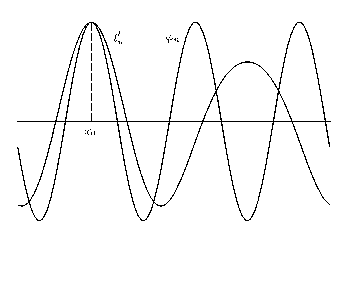
\includegraphics[width=0.5\textwidth]{pict17-1.eps}
\end{center}
 \refstepcounter{ris}\label{r17-1}
 \centerline{���.~\theris}
\end{figure}

 \noindent
 ���ᬮ�ਬ ��१�� $\left[ x_0-\dfrac{\pi}{n}, x_0+\dfrac{\pi}{n}
 \right]=I,$ ��騩�� ����� �� ��������� ��ਮ��� �㭪樨 $\varphi_n.$
 ����뢠���� (�. ��.~\ref{r17-1}), ��
$$
 \varphi_n(x)\le t_n'(x)\qquad \forall\ x\in
 \left[ x_0-\frac{\pi}{n}, x_0+\frac{\pi}{n}\right]=I.
$$
 ������� �� ᢮��⢮ ���㦤���ﬨ  �� ��⨢����. �।�������, �� ������� �窠 $x'\in I,$
 � ���ன $t_n'(x')< \varphi_n(x').$ {����� �� �஬���⪥ $I$ �஬� $x_0$ ��������}
{�� �ࠩ��� ��� �� ���� ��� $x''$ �㭪樨
$t_n'-\varphi_n$ {(�. ��.~\ref{r17-2}).}}

\begin{figure}[ht]
\begin{center}
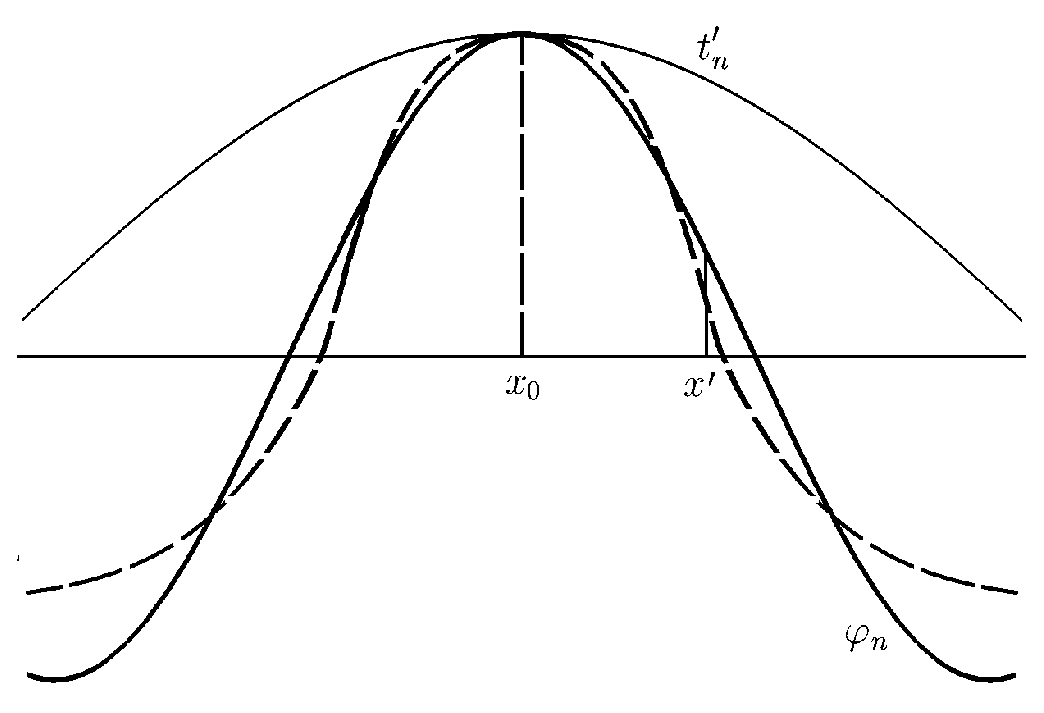
\includegraphics[width=0.5\textwidth]{pict17-2.eps}
\end{center}
% \bigskip
 \refstepcounter{ris}\label{r17-2}

\centerline{���.~\theris}
\end{figure}

%\bigskip

% \noindent
 �㤥� ����� �㫨 ࠧ���� $t_n'-\varphi_n.$  ���ᬮ�ਬ ��१��, �� ������
 $\cos n(x-x_0)$ ���� ࠧ
 ������� �� $-1$ �� 1. �� ������ �� ��� ��१��� ��䨪 $\varphi_n$
 ���ᥪ����� � ��䨪��  $t_n';$
 �� �⮬, �᫨ ����祭�� �����⢫����  � �窥 ����६㬠 $\varphi_n$, �  ��
 �窠 ���� ������ ��୥� ࠧ����  $t_n'-\varphi_n.$ � ��⮬ ��⭮�⥩, ��䨪
 �������� $\varphi_n(x)=M_1 \cos n(x-x_0)$
 ���ᥪ��� ��䨪  $t_n'$ {�� �ࠩ��� ���} �⮫쪮 ࠧ, ᪮�쪮 $\cos n(x-x_0)$
 ��������� �� $-1$ �� 1. ����� ��ࠧ��, ��� �᭮�����
 ��१�� $I$ ������� $2n-2$ ��� ࠧ���� $t_n'-\varphi_n,$
 {�᫨ ��� �� �������� � ����� ��१�� $I$;} �஬� ⮣�,  �� $I$
�������� �� ��� ��� -- � �窥 $x_0$ (������� ���) � � �窥 {$x''\in {\rm int}\, I$}
 (�� �।���������). ����� ��ࠧ��, �� ᤥ������ �������⥫쭮� �।���������
 �ᥣ� �� ��ਮ�� ࠧ����� $t_n'-\varphi_n$ �����
 (� ��⮬ ��⭮��), �� �ࠩ��� ��� $2n-2+2+1=(2n+1)$
 �㫥�. {�᭮, �� �᫨ $x''$ ᮢ������ � ����� �� ���殢 ��१�� $I$ ���
 �㭪�� $t_n'-\varphi_n$}
 {�������� � ����� ��� �����, � ��饥 �᫮ �� �㫥� �� ��ਮ��
 �� 㬥������.}  ������  $t_n'-\varphi_n$ ���� (���㫥���)  �ਣ��������᪨�
 ������� ���浪� $n$
 � �� ����� ����� �⮫쪮 �㫥�  (�� ��ਮ��). ��諨 � ��⨢����. �����,
 ����⢨⥫쭮, �ࠢ������ ��ࠢ���⢮
 $$
 M_1\cos n(x-x_0)\le t_n'(x)\qquad \forall\ x\in
 \left[ x_0-\frac{\pi}{n},x_0+\frac{\pi}{n} \right].
 $$

 �ந�⥣��㥬 ��᫥���� ��ࠢ���⢮ �� $x$ ��
 $ \left[ x_0-\dfrac{h}{2},x_0+\dfrac{h}{2} \right]\subset I$
 �� $0<h<\dfrac{2\pi}{n}.$ � १���� ����稬
 $$
 M_1 \int_{x_0-\frac{h}{2}}^{x_0+\frac{h}{2}}\cos n(x-x_0)\, dx=
 \frac{M_1}{n} 2\sin \frac{nh}{2}\le
 $$
 $$
 \le \int_{x_0-\frac{h}{2}}^{x_0+\frac{h}{2}} t_n'(x)\, dx=
 t_n\left(x_0+\frac{h}{2}\right)- t_n\left(x_0-\frac{h}{2}\right)\le
 \|\Delta_ht_n\|_C
 $$
 �, ⠪ ��� $M_1=\|t_n'\|_C,$ � ����� �� $k=1$ ��������.
 ����� �� $0<h<\dfrac{2\pi}{n}$ ��୮ ��ࠢ���⢮
 $$
 \|t_n^{(k-1)}\|\le \bigg( \dfrac{n}{2\sin\frac{nh}{2}}\bigg)^{k-1}\|\Delta_h^{k-1}
 t_n\|_C.
 $$
 ����� �� $0<h'<\dfrac{2\pi}{n}$ �� �����������
 ��ࠢ�����
 $$\|t_n^{(k)}\|_C\le \dfrac{n}{2\sin\frac{nh'}{2}}\|\Delta_{h'} t_n^{(k-1)}\|_C=
\bigg(
\dfrac{n}{2\sin\frac{nh'}{2}}\bigg)\|(\Delta_{h'}
t_n)^{(k-1)}\|_C\le
$$
$$
\le \bigg( \dfrac{n}{2\sin\frac{nh'}{2}}\bigg)
\left( \dfrac{n}{2\sin nh}\right)^{k-1}\|\Delta_h^{k-1}(\Delta_{h'} t_n)\|.
$$
������� ⥯��� $h'=h\in \Big(0,\dfrac{2\pi}{n}\Big),$
����稬 �ॡ㥬��

%\newpage
 �\;�\;�\;�\;�\;�\;�\;�\;�\;�\;�\;�\;�\;�\quad ⥮६�~\ref{t17-1}.
 �।�⠢�� ࠧ����� $f-t_n$ � ����
 $$
 f-t_n=f-\sigma_{n+p,p}(f)-(t_n-\sigma_{n+p,p}(f)).
 $$
 �த���७��㥬 �� ⮦���⢮ $k$ ࠧ:
 $$
 f^{(k)}-t_n^{(k)}=f^{(k)}-\sigma_{n+p,p}(f^{(k)})-(t_n-
 \sigma_{n+p,p}(f))^{(k)}.
 $$
��� ����砥�
 $$
 \|f^{(k)}-t_n^{(k)}\|_C\le \|f^{(k)}-\sigma_{n+p,p}(f^{(k)})\|_C+\|(t_n-
 \sigma_{n+p,p}(f))^{(k)}\|_C.
 $$
 �ਬ���� ��ࠢ���⢮ ������  (��� ��⮤� ����� ���ᥭ�), �����
 $$
 \|f^{(k)}-\sigma_{n+p,p}(f^{(k)})\|_C\le
 ({\|\sigma_{n+p,p}\|_C^C}+1) E_n(f^{(k)})_C.
 $$
 �����, �ਬ���� ��ࠢ���⢮ ����⥩�� � ����� ��ࠢ���⢮  ������, ����砥�
 $$
 \|(t_n-
 \sigma_{n+p,p}(f))^{(k)}\|_C\le (n+p)^k \|t_n-
 \sigma_{n+p,p}(f)\|_C\le
 $$
 $$
 \le
  (n+p)^k (\|f-t_n\|_C+\|f-
 \sigma_{n+p,p}(f)\|_C)
 \le
 $$
 $$
 \le (n+p)^k \left\{
 \|f-t_n\|_C+({\|\sigma_{n+p,p}\|_C^C}+1)\|f-t_n\|_C\right\} =
 $$
 $$
 =({\|\sigma_{n+p,p}\|_C^C}+2)  (n+p)^k
 \|f-t_n\|_C.
 $$
 ����� ��ࠧ��,  �ࠢ������ ��ࠢ���⢮
 \begin{equation}\label{f17-1}
 \|f^{(k)}-t_n^{(k)}\|_C\le (\|\sigma_{n+p,p}\|_C+2) \left\{ (n+p)^k
 \|f-t_n\|_C+E_n(f^{(k)})_C\right\}. %\eqno(1)
 \end{equation}

 ������� ����� $p=n.$ ��  ⥮६� ������᪮�� ���� $\|\sigma_{2n,n}\|$
 ��࠭�祭� (�� $n$). ���⮬�  �� {\eqref{f17-1}} ᫥��� �業��
 $$
 \|f^{(k)}-t_n^{(k)}\|_C\le A_k \left\{ n^k \|f-t_n\|_C+E_n
 (f^{(k)})_{{C}}\right\}.
 $$
 ���६� ��������.

 \begin{Remark} %%%����砭��.
 �ਢ�������  ������⥫��⢮ ���� ���祭�� $A_k=O(2^k).$ �� ᠬ�� ���� ����� �������   $A_k=O(\ln(k+1)).$
 ��� ���᭮����� �⮣� ����室���   �������騬 ��ࠧ�� �����
 ��ࠬ��� $p.$ �� �業�� {\eqref{f17-1}}  �� ⥮६�
 ������᪮�� ����稬
 $$
 \|f^{(k)}-t_n^{(k)}\|_C\le \left\{ \frac{4}{\pi^2}\ln
 \frac{n+p}{p+1}+O(1) \right\} \left( \frac{n+p}{n}\right)^k \left(
 n^k \|f-t_n\|_C+E_n (f^{(k)})_C\right).
 $$
 ��⥬ �롮� $p=p(n)$ ᤥ���� ����稭�
  \begin{equation}\label{f17-2}
\left\{ \frac{4}{\pi^2}\ln \frac{n+p}{p+1}+O(1)\right\} \left(
 \frac{n+p}{n}\right)^k %\eqno(2)
  \end{equation}
 ��� ����� �����. ���ᬮ�ਬ ��� ����.

 {\Case $k\le n.$} �롥६ 楫�� $p$ ⠪, �⮡� $\dfrac{n}{k}-1\le p\le \dfrac{n}{k}.$
 �����
 $$
 \left( \frac{n+p}{n}\right)^k \le \left( 1+
 \frac{{n}/{k}}{n}\right)^k = \left(
 1+\frac{1}{k}\right)^k\le e,
 $$
 $$
 \frac{n+p}{p+1}=\frac{n-1}{p+1}+1\le k\frac{n-1}{n}+1< k+1.
 $$
 �� ⠪�� �롮� ��ࠬ��� $p$ ����稭� {$\eqref{f17-2}$}
 �㤥� ����� ���祭��   $O(\ln(k+1)),$ �.\,�. $A_k=O(\ln(k+1)).$

 {\Case $k\ge n.$}
 \noindent  ������� $p=0.$ � �⮬ ��砥 ��� ����稭� {$\eqref{f17-2}$}  ����� {�業��}
 $$
 \frac{4}{\pi^2} \ln (n+1)+O(1)\le
 \frac{4}{\pi^2} \ln (k+1)+O(1)=O(\ln(k+1)).
 $$
 �⠪, � ����� ����� ����砥�
 $$
 A_k=O(\ln(k+1)).
 $$
 \end{Remark}

 \task %%% �����.
 ��������, �� ��� ���冷� ����稭� $A_k$ ���� ���.

 \begin{Remark} %%%����砭��.
 ��ࠢ���⢮ ����⥩��~(\ref{17-2}) �������� ���� � ����࠭�⢥ $C_{2\pi}.$
 ������, ��� ����� ��������, ��� ����� ���� � � �� ����த��� ����࠭�⢥. ���⮬� �
 ⥮६�~\ref{t17-1} � ����७�஢���� �ਡ������� ���������
 ��ୠ �� ⮫쪮 � $C,$ �� � � �� ����த��� ����࠭�⢥ (�. ����砭�� � ���� �.~17.1).
 \end{Remark}

 % ���樨 ��ࣥ� ���ᮢ�� ��窨��
% ���ᥭ� ��ࠢ����� �.�.���⮢�, ����� 06.07.2009
% ���ᥭ� ��ࠢ����� �.�.�����, ����� 24.07.2009
% ���ᥭ� �ࠬ����᪠� � ���-�ࠢ�� �.����������, ����� 05.08.09

 %%%%%%%%%%%%%%%%%%%%%%%%%%%%%
 \chapter{�ਡ������� ��⮪���ࠧ�� �।�⠢���� �㭪権}
  %%{����� 18.}



 \section{�ਡ�������  �㭪権 � ����࠭�⢥  $L_{2\pi}$
 %\\ �ਣ��������᪨�� ����������
 }

���ᬮ�ਬ ���砫�  ������襥 �ਡ������� �㭪権 � ����࠭�⢥ $L= L_{2\pi},$
���������� ��ମ�
$$
\|f\|_L=\frac{1}{\pi}\int_{0}^{{2\pi}}|f(t)|dt,
$$ �ਣ��������᪨��
 ����������
 $$
 t_{n-1}(x)=\frac{\alpha_0}{2}+\sum\limits_{k=1}^{n-1} (\alpha_k\cos
 kx+\beta_k \sin kx)
 $$
 ���浪� $n-1,$~ $n\ge 1.$



 \begin{teo}\label{approx_L} \it{ ��� �㭪権  $f\in L_{2\pi}$ �ࠢ������
 ᫥���騥 ��� �⢥ত����:

 $1)$ �᫨ ��� �ਣ��������᪮�� �������� $t_{n-1}^{{*}}$ �㭪��, ࠢ��� ����� ࠧ����
 $R=f-t_{n-1}^{{*}},$ ��⮣����쭠 ����࠭��� ${\cal T}_{n-1}:$
 \begin{equation}\label{f18-1}
 \sign R \perp {t_{n-1}}\qquad \forall\  {t_{n-1}\in\mathcal{T}_{n-1}}, %\eqno(1)
  \end{equation}
 � $t_{n-1}^*$  --  ������� ������襣� �ਡ������� �㭪樨 $f$ � $L_{2\pi}$.


 $2)$ �᫨  $t_{n-1}^{{*}}$ -- ������� ������襣� �ਡ������� �㭪樨 $f$ � ࠧ�����
 $f-t_{n-1}^{{*}}$ ���� ���� �⫨筠 �� ���, � ��易⥫쭮 �믮������
 �᫮���~$(\ref{f18-1}).$}
 \end{teo}

 � ���� ���樨 9 ����ਫ��� � ��������� �뢮�� ���������
 १���� ��� �ਡ������� � $L(Q)$ �� �ਢ�������� ⠬
 ������⥫��⢠ ����� ������� ������襣� �ਡ������� �
 $L^p(Q).$ ���� �ਢ������ ������ ������⥫��⢮ ���
 ��ᬠ�ਢ������ ��⭮�� ����.


 \begin{proof}
 %� � � � � �  � � � � � � � �\ \  � � � � �.
 �।�������, �� ���
 �ਣ��������᪮�� �������� $t_{n-1}^{{*}}$ �믮������ ᢮��⢮~$(\ref{f18-1}),$
 �.\,�.  �㭪�� $\sign R$
 ��⮣����쭠  ��� �������� ���浪� $n-1.$ �����  ��� ��� ��������
 {$t_{n-1}\in {\cal T}_{n-1}$}
 $$
 \|f-t_{n-1}^{{*}}\|_L=\frac{1}{\pi}\int_0^{2\pi} |f(x)-t_{n-1}^{{*}}(x)|\, dx=
 \frac{1}{\pi}\int_0^{2\pi} (f(x)-t_{n-1}^{{*}}(x))\ \sign R(x)\, dx=
 $$
 $$
 =\frac{1}{\pi}\int_0^{2\pi} ((f(x)-{t}_{n-1}(x))+({t}_{n-1}(x)-t_{n-1}^{{*}}(x)))\
 \sign R(x)\, dx=
 $$
 $$
 =\frac{1}{\pi}\int_0^{2\pi} (f(x)-{t}_{n-1}(x))\ \sign R(x)\, dx\le
 \frac{1}{\pi}\int_0^{2\pi} |f(x)-{t}_{n-1}(x)|\, dx=\|f-{t}_{n-1}\|_L.
 $$
�������⥫쭮, $t_{n-1}^{{*}}$ -- ������訩 ������� ��� �㭪樨 $f$ � {$L_{2\pi}$
�।� ��������� �� $\mathcal{T}_{n-1}$.}

�।������� ⥯���, �� $t_{n-1}^{{*}}$ -- ������� ������襣�
�ਡ������� �㭪樨 $f$ � ���� ���� $t_{n-1}^{{*}}\ne f.$ ��� �ந����쭮�� ��������
${t}_{n-1}$ ���浪� $n-1$ ��।���� �㭪��
$$
\Phi(\lambda)=\|f-(t_{n-1}^{{*}}-\lambda {t}_{n-1})\|_L=\frac{1}{\pi}\int_{0}^{2\pi}|f(x)
-t_{n-1}^{{*}}(x)+\lambda {t}_{n-1}(x))|\, dx
$$
����⢥����� ��६������ $\lambda.$
��������, �� �㭪�� $\Phi$ ����७��㥬� � �窥 $\lambda=0$ �
���᫨� �ந������� $\Phi'(0).$

��� ����⢥���� �ᥫ $a\ne 0$ � $b$ �㭪�� $\phi(\lambda)=|a+\lambda b|$ ��६������
$\lambda$  ����७��㥬� � �窥 $\lambda=0$ � $\phi'(0)=b\ \sign a.$ �஬� ⮣�,
����� ���� ��ࠢ���⢮
$$
\left|\frac{|a+\lambda b|-|a|}{\lambda}\right|\le |b|,\qquad \lambda\ne 0.
$$
�ਬ���� ⥮६� ������ � ����࠭⭮� �室�����, ⥯��� ����㤭� 㡥������, �� �㭪��
$\Phi$ ����७��㥬�  � �窥 $\lambda=0$ �
$$
\Phi'(0)=\frac{1}{\pi}\int_{0}^{2\pi}\  {t}_{n-1}(x)\ \sign (f(x)-t_{n-1}^{{*}}(x))\,dx.
$$
� ᨫ� ����६��쭮�� �������� $t_{n-1}^{{*}}$ �窠 $\lambda=0$ ���� �窮� �����㬠
�㭪樨~$\Phi;$ ���⮬�  $\Phi'(0)=0$ � �� ��諨 � ᢮����~$(\ref{f18-1}).$
���६�~\ref{f18-1} ��������.
\end{proof}

 ����⨬, �� �᫨ �믮������ �᫮���~(\ref{f18-1}), �
 $$
 E_{n-1}(f)_L=\frac{1}{\pi}\int_0^{2\pi} (f(x)-t_{n-1}^{{*}}(x))\ \sign R(x)\, dx=
 \frac{1}{\pi}\int_0^{2\pi} f(x)\ \sign R(x)\, dx
 $$
�, �����⥫쭮,
 \begin{equation}\label{f18-2}
 E_{n-1}(f)_L=\frac{1}{\pi}\int_0^{2\pi} f (x)h^*(x)\, dx,%\eqno(2)
 \end{equation}
��� $h^*=\sign R;$ �� �⮬ �㭪�� $h^*$ �������� ᢮��⢠��
$\|h^*\|_{{L^\infty}}\le 1$ � $h^*\perp {t}_{n-1}$ ��� ��� ��������
$t_{n-1}.$



 \begin{teo} %%% ���६�.
 ����� $f\in L_{2\pi}.$ ����� ��� �� �㭪樨 {$h\in L_{2\pi}^\infty$} � ᢮��⢠��
 $$
 \|h\|_{{L^\infty}}\le 1\quad \textit{�}\quad h\perp
 {t}_{n-1}\qquad \forall\ {t}_{n-1}
 $$
 �믮������ ��ࠢ���⢮
  \begin{equation}\label{f18-3}
 E_{n-1}(f)_L\ge \frac{1}{\pi}\int_0^{2\pi} f(x) h(x)\, dx.%\eqno(3)
  \end{equation}
 \end{teo}

 \begin{proof} %%% ������⥫��⢮.
 ����� $t_{n-1}^*$ -- ������� ������襣� �ਡ������� �㭪樨 $f$ � $L.$
 � ᨫ� ��⮣����쭮�� �㭪樨  $h$ ��������� ���浪� $n-1$
 $$
 \frac{1}{\pi}\int_0^{2\pi} f(x)h(x)\, dx=\frac{1}{\pi}\int_0^{2\pi} (f(x)-t_{n-1}^*(x))h(x)\,dx\le
 \frac{1}{\pi}\int_0^{2\pi} |f(x)-t_{n-1}^*(x)|\,dx=E_{n-1}(f)_L.
 $$
  ���६� ��������.
 \end{proof}

\setcounter{corollary}{0}
\begin{corollary}
�।�������, ��  $t_{n-1}^*$ -- ������� ������襣� � $L_{2\pi}$
�ਡ�������  ��� �㭪樨 $f$ �
�㭪��  $h^*=\sign (f-t_{n-1}^*)$ 㤮���⢮���  �᫮���~$(\ref{f18-1})$ $($� �ਬ���,
ࠧ����� $f-t_{n-1}^*$ �� ࠢ�� ��� ���� ����$).$ �����
 $$
 E_{n-1}(f)_L=\frac{1}{\pi}\int_0^{2\pi} f(x)h^*(x)\,dx=
 $$
 $$=\max \left\{\frac{1}{\pi}\int_0^{2\pi} f(x)h(x)\,dx:\
 h\in {L_{2\pi}^\infty},\ \|h\|_{{L^\infty}}\le 1;\ h\perp {t_{n-1}}\
 \forall\ {t_{n-1}}\in {\cal T}_{n-1}\right\}.
 $$
\end{corollary}

\begin{corollary}  �᫨ ������� {$t_{n-1}^*$} ⠪��, ��  ࠧ����� {$f-t_{n-1}^*$} ���� ����
�⫨筠 �� ��� � �㭪�� $h^{{*}}=\sign (f-t_{n-1}^{{*}}) $ ��⮣����쭠
����࠭��� ��������� ���浪� $n-1,$ � {$t_{n-1}^*$} --
������� ������襣� �ਡ������� � $L_{2\pi}$ ��� �㭪樨 $f,$ � ��ࠢ���⢮
{\eqref{f18-3}} �� �㭪樨 $h^{{*}}$ � ⮫쪮 �� �⮩ �㭪樨 ���頥��� �
ࠢ���⢮.
\end{corollary}

\ \

�� �㭪�� $h$ {�� $L_{2\pi}^\infty$} � ᢮��⢠��
$$
\|h\|_{{L^\infty}}\le 1\quad \text{�}\quad h\perp t_{n-1}\qquad \forall\
t_{n-1}\in {\cal T}_{n-1}
$$
���� � ᨫ� {\eqref{f18-3}} ��� ����稭� $E_{n-1}(f)_L$ �業�� ᭨��.
 �롥६ ᯥ樠��� ��ࠧ�� �㭪��  $h.$ �।�������, ��  $h$ ����� ��ਮ�  $\omega=\dfrac{2\pi}{n}$
 � $\ds\int_{-\pi}^{\pi} h(x)\, dx=0.$ ����� �� ���� ⠪�� �㭪樨 ����� ���
  $$
 h(x) \sim \sum\limits_{k=1}^{\infty} \alpha_{nk}\cos nkx+\beta_{nk}\sin nkx,
 $$
 �.\,�. � �㭪樨 $h$ ����� ����  �⫨�� �� ��� ⮫쪮 �����樥���
 ����, ����� ������ ���� ��� $n.$
 � ��⭮��, �믮������ ᢮��⢮
 $$
 h\perp {t}_{n-1}\qquad \forall\  {t}_{n-1}.
 $$
 ���⮬� � ����⢥ $h$ � {\eqref{f18-3}}
 ����� ����� ���� ⠪�� �㭪�� (㤮���⢮������, ������ ⮣�, �᫮���
 {$\|h\|_{L^\infty}\le 1$}).


 ���쬥� �㭪�� $h(x)=\sign \sin(nx+\alpha).$ �� �㭪�� ��������
 �ᥬ� ����᫥��묨 ᢮��⢠��: �� ��ਮ�
  $\omega$ ࠢ�� $\dfrac{2\pi}{n},$~
 $ \dfrac{1}{\pi}\displaystyle\int_{-\pi}^{\pi} h(x)\, dx=0$ � {$\|h\|_{L^\infty}\le 1.$}
 ���⮬�
  \begin{equation}\label{f18-4}
 E_{n-1}(f)_L\ge \frac{1}{\pi}\int_{-\pi}^{\pi} f(x)\, \sign\sin(nx+\alpha)\, dx\qquad
 \forall\ \alpha.%\eqno(4)
  \end{equation}
 ���ᬮ�ਬ ��砨 $\alpha=0$ � $\alpha=\dfrac{\pi}{2}.$ ���� �����⭮ ࠧ�������
 $$
 \sign \sin x=\frac{4}{\pi}\sum\limits_{k=0}^{\infty}\frac{\sin
 (2k+1)x}{2k+1}.
 $$
�������⥫쭮,
 %\addtocounter{equation}{1}
 \refstepcounter{equation}\label{f18-5}
 $$
 \sign \sin nx=\frac{4}{\pi}\sum\limits_{k=0}^{\infty}\frac{\sin
 (2k+1)nx}{2k+1}.\eqno(\theequation')
 $$
 �������筮,
 $$
 \sign \cos x=\sign \sin\left( x+\frac{\pi}{2}\right)
 =\frac{4}{\pi}\sum\limits_{k=0}^{\infty}\frac{(-1)^k\cos
 (2k+1)x}{2k+1},
 $$
 $$
 \sign \cos nx=\frac{4}{\pi}\sum\limits_{k=0}^{\infty}
 \frac{(-1)^k\cos (2k+1)nx}{2k+1}.\eqno(\theequation'')
 $$
 � ᨫ� {\eqref{f18-4}}  ��� �� �㭪樨 $f\in L$ �ࠢ������
 $\Big($����砥�� ᮮ⢥��⢥���, �� $\alpha=0$ � $\alpha=\dfrac{\pi}{2}\Big)$ �業��
 \begin{equation}\label{f18-6}
 E_{n-1}(f)_L\ge \frac{4}{\pi}\sum\limits_{k=0}^{\infty}
 \frac{b_{(2k+1)n}}{2k+1}, %\eqno(6)
 \end{equation}
 \begin{equation}\label{f18-7}
 E_{n-1}(f)_L\ge \frac{4}{\pi}\sum\limits_{k=0}^{\infty}
 \frac{(-1)^k a_{(2k+1)n}}{2k+1}, %\eqno(7)
 \end{equation}
 ��� $a_{(2k+1)n}$ � $b_{(2k+1)n}$ -- ᮮ⢥�����騥 �����ᠬ �����樥��� ����
  �㭪樨 $f.$
    ����⨬, �� �᫨ $\alpha=\pi,$
 � $h(x)=-\sign \sin nx,$ �᫨ $\alpha=\dfrac{3}{2}\,\pi,$
 � $h(x)=-\sign\cos nx,$ � ����稬 ��������� �業��
 $$
 E_{n-1}(f)_{L}\ge
 -\frac{4}{\pi}\sum\limits_{k=0}^{\infty}\frac{b_{(2k+1)n}}{2k+1},
 \eqno(\ref{f18-6}')
 $$
 $$
 E_{n-1}(f)_{L}\ge
 -\frac{4}{\pi}\sum\limits_{k=0}^{\infty}\frac{(-1)^k a_{(2k+1)n}}{2k+1}.
 \eqno(\ref{f18-7}')
 $$

 ��������� �����, ����� ��᫥���� ���� �業�� �������� � ࠢ���⢮?
 ����� $t_{n-1}^*$ -- ������� ������襣� �ਡ������� �㭪樨 $f.$
 �㤥� ��室��� �� ⮣�, ��   ���� ��� ���  �祪 $x\in(-\pi,\pi)$ �믮������ ᢮��⢮ $f(x)-t_{n-1}^*(x)\ne 0.$
 ������⢮ � {\eqref{f18-6}} �������� ⮫쪮 � ⮬ ��砥, ����� (���� ����)
 \begin{equation}\label{f18-8}
 \sign(f-t_{n-1}^*)=\sign\sin nx; %\eqno(8)
 \end{equation}
 ࠢ���⢮ � {\eqref{f18-7}} ����� ����, ⮫쪮 �᫨
 \begin{equation}\label{f18-9}
 \sign(f-t_{n-1}^*)=\sign\cos nx. %\eqno(9)
 \end{equation}
 �������筮, ࠢ���⢮ �~{$(\ref{f18-6}')$ �~$(\ref{f18-7}')$} �㤥�, �����, ᮮ⢥��⢥���,
 $$
 \sign(f-t_{n-1}^*)=-\sign\sin nx, \eqno(\ref{f18-8}')
 $$
 $$
 \sign(f-t_{n-1}^*)=-\sign\cos nx. \eqno(\ref{f18-9}')
 $$


 �।�������, �� �㭪�� $f$ �����뢭� �� ���ࢠ�� $(-\pi,\pi).$
 ����� {\eqref{f18-9} �~$(\ref{f18-9}')$} �������, �� ࠧ�����
 $f-t_{n-1}^*$ ����� ���� � �� � ⮫쪮 �� �窠�, ��� $\cos nx$
 ���頥��� � ���, �, �����, $t_{n-1}^*$ ���௮����� $f$
 � ���� $\cos nx;$ �������筮,~{\eqref{f18-8} �~$(\ref{f18-8}')$}
 ������, �� $t_{n-1}^*$ ���௮����� $f$ � ���� $\sin nx.$
 �� �᫮��� ���௮��樨 -- ����室��� �᫮��� �ࠢ��������
 (��� �����뢭�� �㭪樨) ࠢ���� �~{\eqref{f18-7}, $(\ref{f18-7}')$,
 \eqref{f18-6}, $(\ref{f18-6}')$,}
 ᮮ⢥��⢥���. ������ � �������� ������ ��� ����� �  ������묨.
  ����⢨⥫쭮, �᫨ ������� $t_{n-1}$ ���௮����� �㭪�� $f,$ � �ਬ���, {⮫쪮}
 � ���� $\cos nx$ � ࠧ����� $f-t_{n-1}$
 ����� ���� � ��� ���� � ����� �����, � �~{\eqref{f18-7}
  ���~$(\ref{f18-7}')$}, ᮮ⢥��⢥���,
 ����� ���� ࠢ���⢮ � {$t_{n-1}^*$}
 ���� ������訬 ��������� ��� $f$ {� $L_{2\pi}$.} {� ��� ������}
 $$
 E_{n-1}(f)_L=\frac{4}{\pi}\left|\sum\limits_{k=0}^{\infty}
 \frac{b_{(2k+1)n}}{2k+1}\right|, \eqno(\ref{f18-6}'')
 $$
  $$
 E_{n-1}(f)_L=\frac{4}{\pi}\left|\sum\limits_{k=0}^{\infty}
 \frac{(-1)^k a_{(2k+1)n}}{2k+1}\right|.\eqno(\ref{f18-7}'')
 $$

 ����� ��ࠧ��, �� ����稫� ᯮᮡ ��宦�����
 ������襣� �������� � $L_{2\pi}$ ��� $f\in C_{2\pi}$:
 �롨ࠥ� $h(x)=\sign \sin nx,$ �᫨ $f$ -- ���⭠�, $h(x)=\sign \cos nx,$
 �᫨ $f$ -- �⭠� (��� ��㣨� ��砥� ᫥��� ��ᬮ���� �㭪��
 $\sign \sin (nx+\alpha)$ � ��������� �������� ᮮ⢥�����騬 ��ࠧ�� ���祭�� ��ࠬ���
 $\alpha$). ��⥬ ��ந� �������, �����
 ���௮����� $f$ � ����, ᮮ⢥��⢥���, $\sin nx$ ��� $\cos nx$
 � �஢��塞 ����� ࠧ����. �᫨ ��� 㤮���⢮����
 ᮮ⢥�����騬 �᫮���~{\eqref{f18-8}, $(\ref{f18-8}'),$ \eqref{f18-9} ���~$(\ref{f18-9}')$,}
 � ������訩 ������� ����஥�. ��� �� ����� ����஥���
 ������襣� �������� � $L_{2\pi}$
 ᢮����� � �஢�થ ����� ࠧ���� $f-t_{n-1}^*.$
 �᫨ ����� �� �஢�����, �~{\eqref{f18-7}, $(\ref{f18-7}')$ �~\eqref{f18-6}
 ���~$(\ref{f18-6}')$}
 ���� �業�� ��� $E_{n-1}(f)_L$ ᭨��.


 \section{�ਡ������� ����ᮢ �㭪権 � ${C}_{2\pi}$}

 �����  $K\in L_{2\pi};$ �㭪�� $K$ �㤥� ���뢠��  �㬬��㥬�  �஬.
 ���ᬮ�ਬ ����� �㭪権 $\G M=\G M_K,$  ��⮪���ࠧ�� �।�⠢���� �� �����
 �⮣� ��, �.\,�. �����  �㭪権 ����
 \begin{equation}\label{f18-10}
 f(x)=c+\frac{1}{\pi}\int_0^{2\pi} K(t)\varphi(x+t)\,dt, %\eqno(10)
 \end{equation}
 ���  $\varphi$ -- �ந����쭠� $2\pi$-��ਮ���᪠� �㭪�� �� ����࠭�⢠
 {$L^\infty=L_{2\pi}^{\infty}$}
 � ᢮��⢮� $\|\varphi\|_{{L^\infty}}\le 1,$ � $c=c(f)$ -- ����⢥���� ����⠭�.
 �㭪樨 �� ����� $\G M$ ���� �����뢭묨 $2\pi$-��ਮ���᪨��. ������
  �㭪�� $f\in \G M$
  ������訬 ��ࠧ�� �ਡ����� �ਣ��������᪨��
 ���������� � $C_{2\pi}$ � ���쬥�
 $$
 \sup_{f\in \G M} \min_{t_{n-1}}\|f-t_{n-1}\|_C=E_{n-1}(\G M_K)_C;
 $$
 ��� ����稭� ���뢠�� ������訬 �ਡ�������� ����� $\G M$
 � ����࠭�⢥ $C_{2\pi}$ ������⢮�
 �ਣ��������᪨� ��������� ���浪� $n-1$.

 ��� ��� �ਣ��������᪮�� �������� {$\widetilde{t}_{n-1}$}  �㭪��
 $$
 t_{n-1}(x)=c+ \frac{1}{\pi}\int_0^{2\pi} \-{\widetilde{t}_{n-1}(t)} \varphi(x+t)\, dt
 $$
⠪�� ���� �ਣ��������᪨� ���������  ���浪� $n-1$, � ��� ���� ��
$c=c(f)$ �����
 $$
 |f(x)-t_{n-1}(x)|=\left| \frac{1}{\pi}\int_0^{2\pi} \{ K(t)-{\widetilde{t}_{n-1}(t)}\}
 \varphi(x+t)\, dt \right|\le \frac{1}{\pi}\int_0^{2\pi} | K(t)-{\widetilde{t}_{n-1}(t)}|\, dt,
 $$
�, �����,
 $$
 \|f-t_{n-1}\|_C\le \frac{1}{\pi}\int_0^{2\pi} |K-{\widetilde{t}_{n-1}}|\,
 dt \qquad \forall \ {\widetilde{t}_{n-1}}.
 $$
 ��� �����砥�, ��
 $$
 E_{n-1}(f)_C\le E_{n-1}(K)_L\qquad \forall \ f\in \G M_K.
 $$
 �������⥫쭮, ����� ���� ��ࠢ���⢮
 \begin{equation}\label{f18-11}
 \sup_{f\in \G M_K} E_{n-1}(f)_C \le E_{n-1}(K)_L. %\eqno(11)
 \end{equation}
{����� 㪠���� �ப�� ����� 拉� $K,$ ����� �� ᠬ�� ���� ����� ����� ���� ࠢ���⢮;
���� �� �㤥� ᤥ���� ��� ������� �����⭮�� ����.}

 �ਢ������ ��� ���㦤���� ����� ������� � �� ����த���
 ����࠭�⢥ $H$ $2\pi$-��ਮ���᪨� �㭪権, ��ଠ � ���஬ ����ਠ�⭠ �⭮�⥫쭮 ᤢ���.
 ����� �㤥�  �����
 $$
 \|f-t_{n-1}\|_H=\left\| \frac{1}{\pi}\int_0^{2\pi}\{K(t)-{\widetilde{t}_{n-1}(t)}\}
 \varphi(x+t)\, dt\right\|_H\le
 $$
 $$
 \le \frac{1}{\pi}\int_0^{2\pi} |K(t)-{\widetilde{t}_{n-1}(t)}|\ \|\varphi(\cdot +t)\|_H\, dt=
 \frac{1}{\pi}\int_0^{2\pi} |K(t)-{\widetilde{t}_{n-1}(t)}|\, dt \cdot \|\varphi\|_H
 $$
 �, ᫥����⥫쭮,
 $$
 E_{n-1}(f)_H \le E_{n-1}(K)_L\cdot \|\varphi\|_H.
 $$
 ������稬 �१  $\G M_{K,H}$ ����� �㭪権 � $H$ ���� {\eqref{f18-10}},
 �  ������ $\varphi\in H,$~ $\|\varphi\|_H\le 1.$ ����� ����稬
 $$
 \sup_{f\in \G M_{K,H}} E_{n-1}(f)_H\le E_{n-1}(K)_L.
 $$
 � ��饬 ��砥 ����� ࠢ���⢠ �� �㤥�.

 \section{�ਡ������� �� ���㫫�\\ �ਣ��������᪨�� ���������� � �।���}



 ������ ��ᬮ�ਬ ����� ${W_1^{(r)}},$~ $r\ge 1,$ �㭪権 $f\in C_{2\pi},$
 � ������ �ந������� $f^{(r-1)}$
 ���浪� $r-1$ �ਭ������� ������ ${\rm Lip\ }1$ � ����⠭⮩ $1,$
 �.\,�. 㤮���⢮��� �᫮���
 $$
 |f^{(r-1)}(x')-f^{(r-1)}(x'')|\le |x'-x''|\qquad \forall\ x',x''.
 $$
 � �㭪樨 $f\in {W_1^{(r)}}$ ���� ����  ������� �ந�������  $f^{(r)}$ ���浪� $r,$
  �� �⮬ $|f^{(r)}(x)|\le 1$ ���� ���� �
 $$\frac{1}{\pi}\int_0^{2\pi}f^{(r)}(x)\, dx=0,$$
 �.\,�. �ந������� $f^{(r)}$
 ����� �㫥��� �।��� ���祭�� �� ��ਮ��. �㭪�� $f\in {W_1^{(r)}}$  ����᪠�� ᫥���饥 ��⥣ࠫ쭮�
 �।�⠢�����:
 \begin{equation}\label{f18-12}
 f(x)=\frac{a_0}{2}+\frac{1}{\pi}\int_{-\pi}^{\pi} K_r(t) f^{(r)}(x+t)\, dt, %\eqno(12)
 \end{equation}
 ��� $\dfrac{a_0}{2}=\dfrac{1}{2\pi}\displaystyle\int_0^{2\pi}f(x)\,dx$
 -- �।��� ���祭�� �㭪樨 $f,$ �
 \begin{equation}\label{f18-13}
 K_r(t)=\sum\limits_{n=1}^{\infty}\frac{\cos\left( nt+\frac{r\pi}{2}\right)} {n^r}. %\eqno(13)
 \end{equation}
 �㭪�� $K_r$ ���뢠�� �஬ ���㫫�.

 �� $r=1$ �����
 $$
 K_1(t)=-\sum\limits_{n=1}^{\infty}\frac{\sin nt}{n}=\frac{t-\pi}{2},\qquad
 t\in (0,2\pi).
 $$
 �� $r>1$ ��  $K_r$  ����砥��� ��⥣�஢����� ��  $K_{r-1}$ � �᫮���� �롮� ����⠭�� ��⥣�஢���� ⠪, �⮡� �।��� ���祭�� �뫮 ࠢ�� ���:
 $$
\frac{1}{2\pi} \int_0^{2\pi} K_r(t)dt=0.
 $$




 � ᨫ� १���⮢ �।��饣� ��ࠣ�� ��� �㭪権 $f\in {W_1^{(r)}}$ �ࠢ������ ��ࠢ���⢮
 $$
 E_{n-1}(f)_C\le E_{n-1}(K_r)_L.
 $$
 ���᫨� ����稭� $E_{n-1}(K_r)_L.$ ����� $K_r$ ��� 㤮��� ���᫨�� ������襥 �ਡ������� �㭪樨
 $$
 K_r(t+\pi)=\sum\limits_{n=1}^{\infty}(-1)^n\frac{\cos\left( nt+\frac{r\pi}{2}\right)} {n^r},
 $$
 ��� �㭪�� ����� ������稬 ᨬ����� $K_r.$ � ᨫ� ᢮��⢠ $2\pi$-��ਮ��筮��
 ����稭� ������襣� �ਡ������� �� �⮬ �� ���������. � ����� ������祭��� �����
 $$
 K_1(t)=\frac{t}{2},\qquad t\in (-\pi,\pi).
 $$
�㭪�� $K_r$ ���� ���⭮� ��� �⭮� � ᮮ⢥��⢨� � ⥬, �㤥� �� �᫮ $r$ ����� ��� ���.

����ந� ��� 拉�  $K_r$
 ���௮��樮��� �������� $U_{n-1}$ � 㧫��� � ���� $\sin nx$, �᫨ �᫮ $r$ ���⭮�,
 � � ����  $\cos nx$, �᫨ �᫮ $r$ �⭮�.
 �������� ��� ����� ��⮨� � ⮬, �⮡� ��������, �� ࠧ�����  $R=K_r-U_{n-1}$
 ����� ���� ���� � �窠� ���௮��஢����.
 � ��砥 $r=1$ �㭪�� $K_1$ (�. ��.~\ref{r18-1}) ����� ࠧ��� � �窠� $(2k+1)\pi;$ �� �窨 ᫥���
 ����� �窠�� ��६��� ����� ࠧ���� $R.$
 � ��砥  $r=2s+1,$~ $s>0,$  �窨 $\pm\pi$ ����뢠���� �� � �������⥫�묨 㧫���
 ���௮��஢����.

\begin{figure}[ht]
\begin{center}
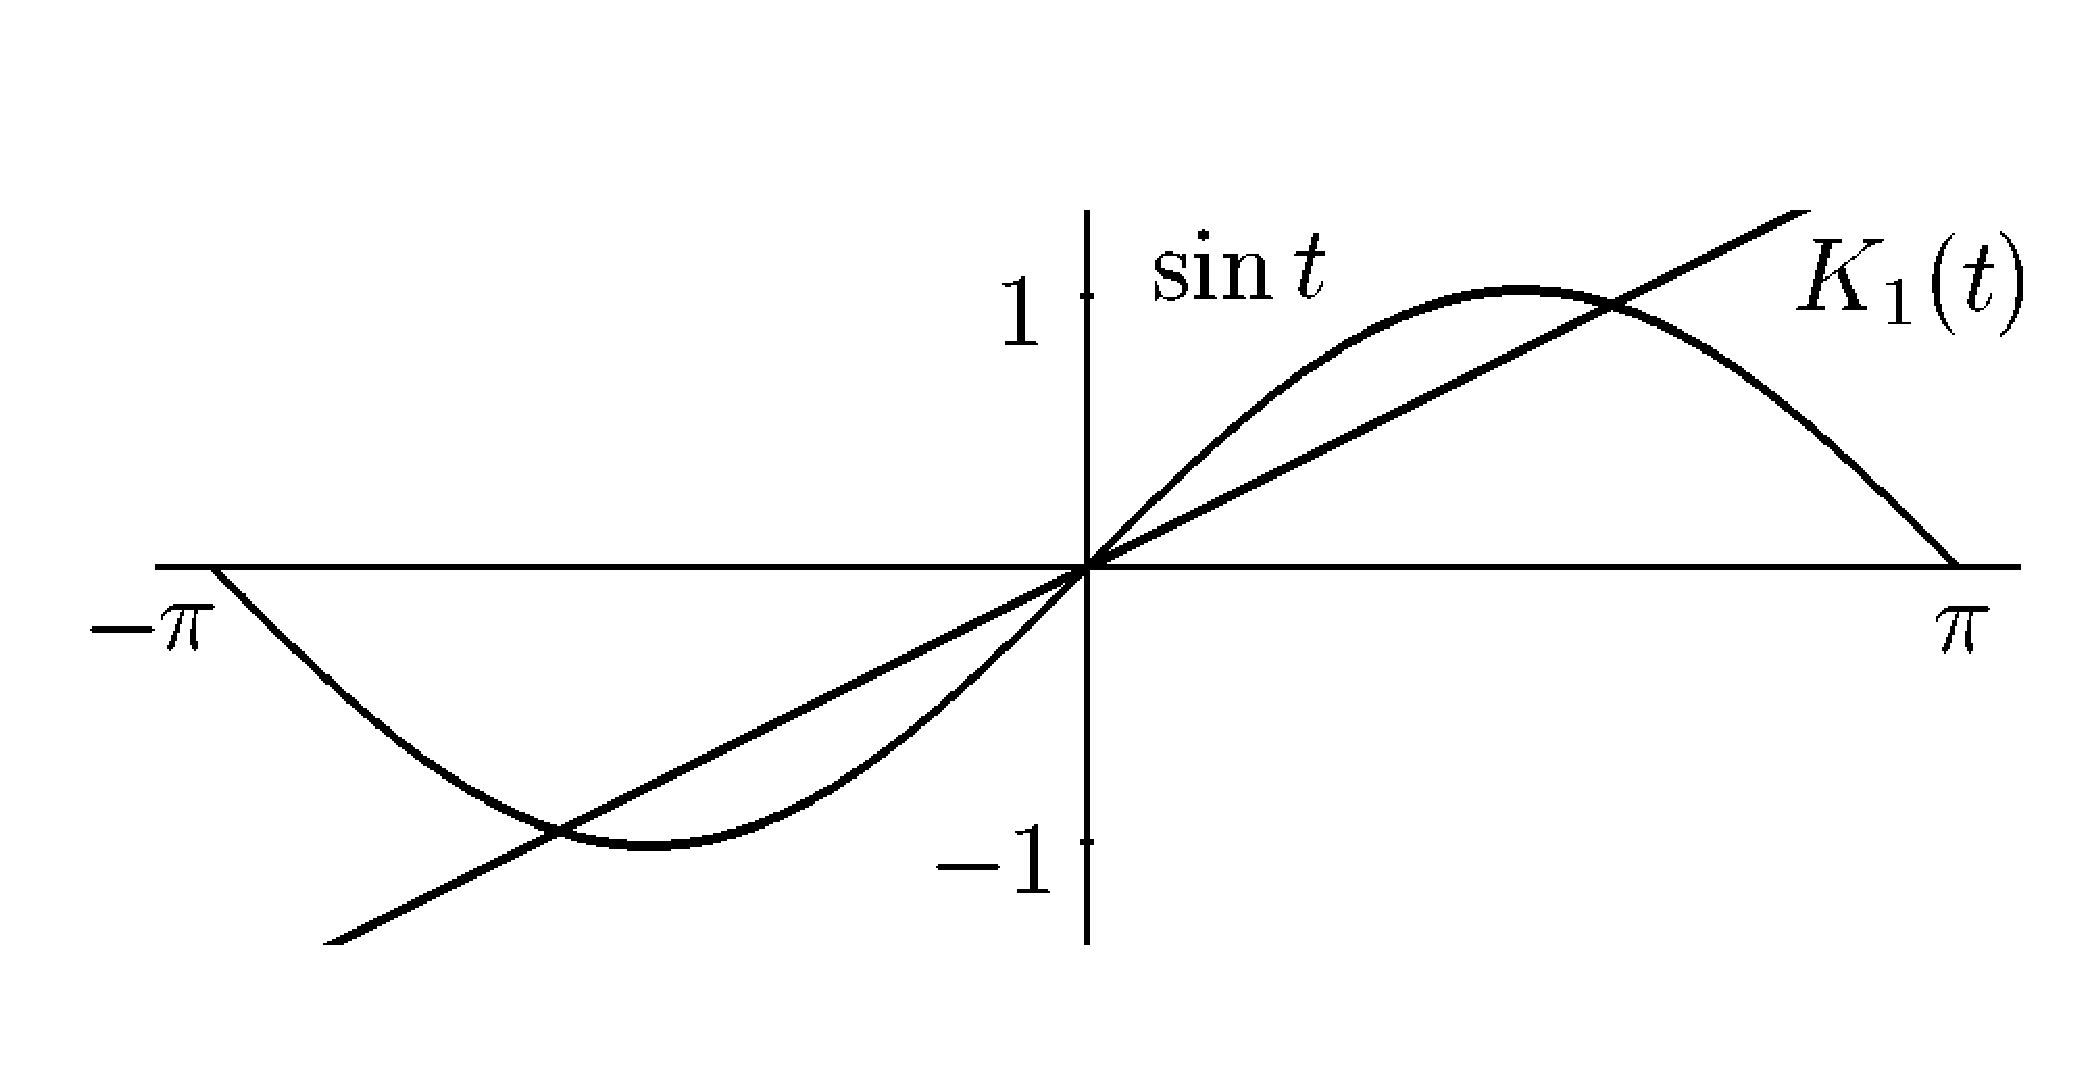
\includegraphics[width=0.5\textwidth]{pict18-1.eps}
\end{center}
 \refstepcounter{ris}\label{r18-1}

 \centerline{���.~\theris}
\end{figure}





 \begin{lemma}\label{l18-2}
 �������� $R=K_r-U_{n-1}$ �� $K_r$ � ���௮��樮�����
 ��������
 $U_{n-1}$ �������� ᢮��⢮�
 $$
 \sign(K_r(t)-U_{n-1}(t))=\pm \sign \sin nt,\qquad t\in(-\pi,\pi),
 $$
  �᫨ �᫮ $r$ ���⭮�, � ᢮��⢮�
 $$
 \sign(K_r(t)-U_{n-1}(t))=\pm \sign \cos nt,\qquad t\in(-\pi,\pi),
 $$
  �᫨ �᫮ $r$ �⭮�.
 \end{lemma}

�\;�\;�\;�\;�\;�\;�\;�\;�\;�\;�\;�\;�\;�\quad �����~\ref{l18-2}.
�������� $R=K_r-U_{n-1}$ �� $(-\pi,\pi)$ ����� $(2n-1)$ �㫥� �� ���⭮� $r$ �
$2n$ �㫥� -- �� �⭮� $r.$ ��� ���᭮����� �⢥ত���� ����� �����筮
��������, �� �� �� �㫨 ����� � ��㣨� �㫥� ���.

� ᢮� ��।�, ��� �⮣� �����筮 ��������, �� �� $r$ ���⭮�
��� �ந����쭮�� ���⭮�� �ਣ��������᪮�� �������� $V_{n-1}$ ���浪� $n-1$ ࠧ�����
$R=K_r-V_{n-1}$ ����� �� $(-\pi,\pi)$ �� ����� $(2n-1)$ �㫥� (� ��⮬ ��
��⭮��), � �� �⭮� $r$ � �⭮� �������� $V_{n-1}$
ࠧ����� $R=K_r-V_{n-1}$  ����� �� $(-\pi,\pi)$ �� �����
$2n$ �㫥� {(����� �� � ��⮬ ��
��⭮��).} ������� �� �⢥ত����  ����樥� �� $r\ge 1.$


1. ����� $r=1.$ �������, �� ࠧ����� $R=K_1-V_{n-1}$ ����� �஬ $K_1$ (��� � ������
��砥 ���⭮�) � ����� �ਣ��������᪨�
  ��������� $V_{n-1}$ ����� �� ���ࢠ�� $(-\pi,\pi)$ �� ����� $(2n-1)$
  �㫥� (� ��⮬ �� ��⭮��).
  ������� ��� 䠪� �� ��⨢����. �ந������� ࠧ����
 $$
 R'(t)=\frac{1}{2} -V_{n-1}'(t)=\frac{1}{2} -\sum\limits_{k=1}^{n-1}
 \alpha_k\cos kt,\qquad t\in (-\pi,\pi),
 $$
 ���� (���㫥���) ������� ��  ��ᨭ�ᠬ ���浪� $n-1$. ����� �������
 ����� ����� �� $(-\pi,\pi)$
 �� ����� $(2n-2)$ �㫥�. �᫨ �� �� $(-\pi,\pi)$ ࠧ����� $R$ �����,
 �� �ࠩ��� ���,  $2n$
 �㫥�, � �� ⥮६� ����� �� �ந�������  $R'$ ����� �� $(2n-1)$
 �㫥�, 祣� ���� �� �����. ��諨 � ��⨢����. �������⥫쭮,
 $R=K_r-V_{n-1},$ ����⢨⥫쭮,
 ����� �� $(-\pi,\pi)$ �� ����� $(2n-1)$ �㫥�.

 2. ����� $r=2.$ ���  $K_2$ � ������� $V_{n-1}$  ����� ��묨.
 �� �⨬  ��������, �� ࠧ�����
 $R=K_2-V_{n-1}$ ����� �� $(-\pi,\pi)$
 �� ����� $2n$ �㫥�.
 �����  $R'=K_2'(t)-V'_{n-1}$, ���
 $V'_{n-1}$ ����  ����� ������� ���浪� $n-1$. ���쪮 ��  �� 㦥 ��������, �� ⠪��
 ࠧ����� ����� ����� �� ����� $(2n-1)$ �㫥� �� $(-\pi,\pi).$
 �������⥫쭮, $R$ ����� ����� �� ����� $2n$ �㫥�.

 3. ������� ⥯���, �� �᫨ ��  $r>1$ �㦭�� ᢮��⢮ �㫥�  ����� ���� ��� ����� $r-1,$ � ��� ����� ���� � ��� ����� $r.$    ����� $r>1$ ���⭮�,
 $r=2s+1,$~ $s\ge 1.$
 ����� $K_{2s+1}$ � $V_{n-1}$ ����� �, ᫥����⥫쭮  $K_{2s+1}$
 � $V_{n-1}$ �������� � �窠� $\pm \pi$
 � ���. �� ⮣�� � ࠧ�����  $R=K_{2s+1}-V_{n-1}$ ⠪�� � ��� �窠� ���頥��� � ���:
 $R(\pm \pi)=0.$
  �������, �� �᫮ �㫥� $m$ ࠧ����  $R$ �� $(-\pi,\pi)$ �� �ॢ��室��
  $2n-1.$ ��᪮��� $R(\pm\pi)=0,$ � �� ⥮६� ����� �ந������� $R'$
   �㤥� �����  $m+1$ ��� �� ���ࢠ�� $(-\pi,\pi).$ ��  �।��������� ��
   ����樨 �ந�������  $R'=K_{r-1}-V'_{n-1}$
 ����� �� $(-\pi,\pi)$ �� ����� $2n$ �㫥�. �������⥫쭮,  �᫮ �㫥�
 ࠧ����  $R=K_{2s+1}-V_{n-1}$ �� �ॢ��室�� �᫠ $2n-1.$


 �᫨ $r=2s$ �⭮�, � $R'=K_{2s-1}-V'_{n-1}$ ���� �㭪�� ���⭠� � �� ������⥫����
  ����� �� ����� $(2n-1)$ �㫥�. �� ⥮६� �����  ࠧ����� $R$ ����� �� ����� $2n$
 �㫥�. ����� ��������.

 ������ ����� �믨��� ������襥 �ਡ������� �� ���㫫� {\eqref{f18-13}} �ਣ��������᪨�� ���������� �
 �।���.

 \begin{teo}\label{t18-2}
 ������� $U_{n-1}$ ���浪� $n-1,$ ���௮�����騩 ��  $K_r$
 � ���� $\sin nx$, �᫨ �᫮ $r$ ���⭮�, � � ����  $\cos nx$, �᫨ �᫮ $r$ �⭮�,
 ���� ��������� ������襣� �ਡ������� ��� $K_r$ � ����࠭�⢥ $L;$ �� �⮬
 \begin{equation}\label{f18-14}
 E_{n-1}(f)_L=\|K_r-U_{n-1}\|_L=\frac{M_r}{n^r}, %\eqno(14)
 \end{equation}
 ���
 \begin{equation}\label{f18-15}
 M_r=\frac{4}{\pi}\sum\limits_{k=0}^{\infty}
 \frac{(-1)^{(r+1)k}}{(2k+1)^{r+1}}. %\eqno(15)
 \end{equation}
 \end{teo}




  �\;�\;�\;�\;�\;�\;�\;�\;�\;�\;�\;�\;�\;�\quad ⥮६�~\ref{t18-2}.
  ����६��쭮��� ��������� $U_{n-1}$ �뫠 ���᭮���� � �।������� ���㦤�����.
  �����, �ਬ���� ����~{$(\ref{f18-6}''),$ $(\ref{f18-7}'')$}, {{$(\ref{f18-5}'),$
  $(\ref{f18-5}'')$}} � ࠧ�������~{\eqref{f18-13},}  ����砥�
  $$
 E_{n-1}(f)_L=\left|\frac{1}{\pi}\int_{-\pi}^{\pi}K_r(t)\sign \sin nt\,dt\right|=  \frac{4}{\pi}\, \sum\limits_{k=0}^{\infty}
 \frac{1}{n^r(2k+1)^{r+1}},\qquad r - \mbox{���⭮�},
  $$
  $$
 E_{n-1}(f)_L=\left|\frac{1}{\pi}\int_{-\pi}^{\pi}K_r(t)\sign \cos nt\,dt\right|= \frac{4}{\pi}\, \sum\limits_{k=0}^{\infty}
 \frac{(-1)^{k}}{n^r(2k+1)^{r+1}},\qquad r - \mbox{�⭮�}.
 $$
 ���६� ��������.


\ \

 % ���樨 ��ࣥ� ���ᮢ�� ��窨��
% ���ᥭ� ��ࠢ����� �.�.���⮢�, ����� 06.07.2009
% ���ᥭ� ��ࠢ����� �.�.�����, ����� 24.07.2009
% ���ᥭ� �ࠬ����᪠� � ���-�ࠢ�� �.����������, ����� 05.08.09

 %%%%%%%%%%%%%%%%%%%%%%%%%%%%%
 \chapter{���६� ����� � �� �ਫ������}
 %%{����� 19.}

 \section{���६� �����\\ � �ਡ������� ����७��㥬��
 �㭪権}


 �� ��諮� ���樨 ��  �ਡ������ �㭪樨, ��⮪���ࠧ��
 �।�⠢��� � ������� �� $K\in L_{2\pi},$
 �ਣ��������᪨�� ����������; � �裡 � �⨬  �᪠��
 ������襥 �ਡ������� ��
 $$
 E_{n-1}(K)_L=\min_{t_{n-1}}\|K-t_{n-1}\|_L=\|K-t_{n-1}^*\|_L
 $$
 �ਣ��������᪨�� ���������� � $L_{2\pi}.$ ������訬
 ��������� ��� ���� �������, ���௮�����騩 �㭪�� $K$ �
 ࠢ��������� 㧫�� �  ����ﭨ�� $\dfrac{\pi}{n}$ ����� �ᥤ���� 㧫���.
 ��, � ��⭮��, �ࠢ������ ��� �� ���㫫� $K_r,$ ���஥ ����
 ��⥣ࠫ쭮� �।�⠢����� $r$ ࠧ ����७��㥬�� �㭪権, �筥�, �㭪権 �� �����
  $W^{(r)}$:
 $$
 f(x)=\frac{a_0}{2}+\frac{1}{\pi}\int_0^{2\pi} K_r(t)\varphi(x+t)\, dt,
 $$
 ����� $\varphi=f^{(r)}.$ � �⮬ ��砥, ��� �� �������� �
 ⥮६�~\ref{t18-2},
 $$
  E_{n-1}(K)_L=\| K_r-t_{n-1}^*\|_L=\frac{M_r}{n^r},
 $$
 ��� $M_r$ --  ����⠭��, ��।������  ��㫮� \eqref{f18-15} �।��饩 ���樨.
 %����� ��������, ��  $1<M_r<\frac{\pi}{2}.$

\ \


���� �����饩 ���樨 ��⮨� � ⮬, �⮡�

 1) ��� �㭪樨 $f\in C_{2\pi}^{(r)}$  �業���  ������襥 �ਡ������� $E_{n-1}(f)_C$
 �ਣ��������᪨�� ���������� ���浪� $n-1;$

 2) ���᫨��
 $$
 \sup_{{W_1^{(r)}}} E_{n-1}(f)_C=E_{n-1}(W_1^{(r)})_C,
 $$
 ��� $W_1^{(r)}$ -- ����� �㭪権 $f\in W^{(r)},$ ��� ������
 $\|f^{(r)}\|_{L^\infty}\le 1.$

 �᭮, �� �᫨ ��᫥���� ����� �襭�, � ��� �� �㭪樨 $f\in C^{(r)}$
 ����� ���� ��ࠢ���⢮
 $$
 E_{n-1}(f)_C\le E_{n-1}(W_1^{(r)})_C\cdot \|f^{(r)}\|_C.
 $$
 ����� $t_{n-1}^*$ -- ������� ������襣� �ਡ�������  � �।��� �� $K_r.$
 �����
 \begin{equation}\label{f19-1}
 \int_0^{2\pi} \{ K_r(\theta)-t_{n-1}^{*}(\theta)\}\varphi(x+\theta)
 \,d\theta=f(x)-t_{n-1}(x),%\eqno(1)
 \end{equation}
 ���  $t_{n-1}$ -- ������� �ਣ��������᪨� ������� ���浪� $n-1.$ �, �����,
 \begin{equation}\label{f19-2}
 E_{n-1}(f)_C\le \|f-t_{n-1}\|_C\le \int_0^{2\pi}
 |K_r(t)-t_{n-1}^{*}(t)|\, dt\cdot \|f^{(r)}\|_C. %\eqno(2)
 \end{equation}
 ��� ᫥��� �業��
 \begin{equation}\label{f19-3}
 E_{n-1}(W_1^{(r)})_C\le E_{n-1}(K)_L. %\eqno(3)
 \end{equation}
 �� ᠬ�� ���� ����� ����� ���� ࠢ���⢮, �.\,�. �ࠢ������ ᫥���饥 �⢥ত����.

 \begin{teo}[�����] ��� ���� $n\ge 1,$~ $r\ge 1$
 $$
 E_{n-1}(W_1^{(r)})_C= E_{n-1}(K_r)_L.
 $$
 \end{teo}

����� \eqref{f19-3}, ��� ������⥫��⢠ ⥮६�  �����筮 ��������,
 �� ����� ���� ��ࠢ���⢮
 $$
 E_{n-1}(W_1^{(r)})_C\ge E_{n-1}(K_r)_L.
 $$
 � �⮩ 楫�� ����ந� �㭪�� $f^*\in W_1^{(r)},$ ��� ���ன
 $E_{n-1}(f^*)_C=E_{n-1}(K_r)_L.$
 ���쬥� � {\eqref{f19-1}} ������訩 � �।��� �������
 $t_{n-1}^*$ ��� $K_r.$ ��������, �� �㭪�� $\varphi^*=\sign (K_r-t_{n-1}^*)$
 ���� �ந������� ���浪� $r\ge 1$ �����ன �㭪樨 ��
 $W_1^{(r)}.$

 ��࠭�祭��� ����ਬ�� $2\pi$-��ਮ���᪠� �㭪�� $\varphi$
 ����  �ந������� ���浪� $r\ge 1$ �����ன �㭪樨 ��
  $W^{(r)}$ � ⮬ � ⮫쪮  ⮬ ��砥, �᫨  �।��� ���祭�� �㭪樨
  $\varphi$ ࠢ�� ���. � ��襬
 ��砥, ��� �� �����, $\sign (K_r-t_{n-1}^*)=\sign \sin(nx+\alpha)$
 ��� ᮮ⢥�����饣� ���祭�� $\alpha,$ � ��⮬� $\displaystyle\int_0^{2\pi}\sign \{
 K_r-t_{n-1}^*\}\, dx=0.$ �����, �㭪�� $\varphi^*=\sign(K_r-t^*_{n-1})$
 ���� �ந������� ���浪� $r$  �����ன �㭪樨 $f^*\in W_1^{(r)};$
 ��� �㭪��  ����� ����⠭����� �� ��㫥 (�.~(\ref{f18-12}) � ��⮬
 ������७���� � ᨬ���� $K_r$)
 $$
 f^*(x)=\int_0^{2\pi}\, K_r(\theta-\pi)\,
 \varphi^*(x+\theta)\, d\theta.
 %\eqno(\star)
 $$


 ����� ᢮��� �㭪樨  $\varphi^*(x)=\sign \sin(nx+\alpha),$ �ࠢ������ ᮮ⭮襭��
 $$
 f^*\left( x+\frac{\pi}{n}\right)=-f^*(x),\qquad x\in(-\infty,\infty);
 $$
� �����, �㭪�� $f^*$ ����� �� $[0,2\pi)$ 祡�襢᪨� $2n$-����
����ୠ��. �� 祣� ᫥���, �� ������� ������襣� ࠢ����୮�� �ਡ�������
�㭪樨 $f^*$ ���� ⮦���⢥��� ��� � ��⮬�
 $$
 E_{n-1}(f^*)_C=\|f^*\|_C=\int_0^{2\pi}
 |K_r(t)-t_{n-1}^*(t)|\, dt=E_{n-1}(K_r)_L.
 $$
 �������⥫쭮, $E_{n-1}({W_1^{(r)}})_C=E_{n-1}(K_r)_L.$
 ���६� ��������.

 �⠪, ��������, ��
 $$
 E_{n-1}({W_1^{(r)}})_C=E_{n-1}(K_r)_L=\frac{M_r}{n^r}.
 $$
 ����⠭�� $M_r$ ����� �뫨 ���᫥�� ����஬ � ���뢠����
 ����⠭⠬� �����.  �����
 $$
 M_2=\frac{\pi}{8}\le M_r\le M_1=\frac{\pi}{2},\qquad r\ge 1;
 \qquad \lim_{r\to +\infty}M_r=\frac{4}{\pi}.
 $$





 ��� �� �㭪樨 $f\in C^{(r)}_{2\pi}$
 ⥯��� ����� �������
 \begin{equation}\label{f19-4}
 E_{n-1}(f)_C \le \frac{M_r}{n^r} \|f^{(r)}\|_C. %\eqno(4)
 \end{equation}
 �� ��ࠢ���⢮ ���뢠�� ��ࠢ���⢮� �����.

 �ਬ���� ��ࠢ���⢮ ����� � �㭪樨 $f-t_{n-1},$ ��� $t_{n-1}$
 -- �� ������� ���浪� $n-1;$ ����稬
 $$
 E_{n-1}(f)_C \le \frac{M_r}{n^r} \|f^{(r)}-t_{n-1}^{(r)}\|_C.
 $$
 ����稭� $\|f^{(r)}-t_{n-1}^{(r)}\|,$ ����� ������, ��� ��� $t_{n-1}$
 �����, 祬 $E_{n-1}(f^{(r)})_C,$
 ⠪ ��� $t_{n-1}^{(r)}$ ����� �㫥���  �।��� ���祭��. �������
 $t_{n-1}^{(r)}$ ������訬 ��ࠧ��, ����� �業���
 \mbox{$\|f^{(r)}-t_{n-1}^{(r)}\|_C$} ⮫쪮 �१ $2E_{n-1}(f^{(r)})_C,$
 ⠪ ��� ᢮����� 童� � �������� ������襣� �ਡ������� �ந������� $f^{(r)}$
 �業������� ����稭��  $E_{n-1}(f^{(r)})_C.$ {������ �����}
 {������� �業�� ��������� ���������� �� ��譥� ������.}

 {����⢨⥫쭮,} ��� �� �㭪樨 $f\in C^{(r)}_{2\pi}$ � �ந����쭮��
 �ਣ��������᪮�� �������� $\tau_{n-1}$ �ࠢ������  �।�⠢�����
 $$
 f(x)-{t}_{n-1}(x) =\int_0^{2\pi} \{
 K_r(t)-t_{n-1}^*\}\{\varphi(x+t)-\tau_{n-1}(x+t)\}\, dt,\qquad \varphi=f^{(r)},
 $$
 � ���஬ {$t_{n-1}$} -- ������� �ਣ��������᪨� ������� ���浪� $n-1$,
 {ᮮ⢥�����騩 �������� $\tau_{n-1}$}.
 ��ࠢ � ����⢥  $\tau_{n-1}$ ������� ������襣� ࠢ����୮�� �ਡ������� �㭪樨
 \mbox{$\varphi=f^{(r)}$} � $C_{2\pi},$
 ����稬 ������� {$t_{n-1},$} ��� ���ண�
 $$
 \|f-{t}_{n-1}\|_C\le \frac{M_r}{n^r} E_{n-1} (f^{(r)})_C.
 $$
 �������⥫쭮, ����� ���� ��ࠢ���⢮
 \begin{equation}\label{f19-5}
 E_{n-1}(f)_C\le \frac{M_r}{n^r} E_{n-1}(f^{(r)})_C. %\eqno(5)
 \end{equation}
 %��� �� ���祭�� �������� �ਡ������� �㭪権 $f\in C^{(r)}$  ᢮����� � ���祭�� �������� �ਡ�������  ������७��㥬�� �㭪権.

 ��ࠢ���⢮ \eqref{f19-5} �ࠢ������ � ��� ��㣨� {(������᪨�)}
 ����࠭��, �� �� ��� ������ �� ����࠭�� {$L_{2\pi}^p$~ $(1\le p<\infty)$}
 ����⠭� $M_r$ �� ���� �筮�.

 ���ᬮ�ਬ ����� �ਫ������ ��ࠢ���⢠ �����.

 %\section{�ਫ������ ��ࠢ���⢠ �����}

 \section{����饭�� ��ࠢ���⢠ ����⥩�� \\ ��
 ����७��㥬� �㭪樨}

 %\task %%%�����.
 ����� {$f\in C^{(r)}_{2\pi}.$} �業�� ���� $\|f^{(r)}\|_C$ �१ $\|f\|_C.$

 �᫨ $f=t_n,$ � ����� ���� ��ࠢ���⢮ ����⥩��
 $$
 \|f^{(r)}\|_C\le n^r \|f\|_C,
 $$
 ���஥ ���頥��� � ࠢ���⢮, ���ਬ��, �� �㭪樨 $f(x)=\sin nx.$
 �᫨ $f\ne t_n,$ � ��ࠢ���⢮ ����⥩�� 㦥 �� ����� ����.
  �� ᠬ�� ����
 ����� ���� ᫥���饥 �⢥ত����.

 \begin{teo}\label{t-o-bern} �� $r\ge 1$ ��� �㭪権 {$f\in C^{(r)}_{2\pi}$}
 ����� ���� ����饭��� ��ࠢ���⢮ ����⥩��
 \begin{equation}\label{f19-6}
 \|f^{(r)}\|_C\le n^r\|f\|_C+A_rE_n(f^{(r)})_C, %\eqno(6)
 \end{equation}
 ��� $A_r$ ���� ������� ����⠭�, �������� ⮫쪮 �� $r.$
 \end{teo}



 �᫨ $r$ 䨪�஢���, � $n\to \infty,$ � $E_n(f^{(r)})_C\to 0$ �
 $A_rE_n(f^{(r)})_C$ ���� �� ������ $n.$

 %�\;�\;�\;�\;�\;�\;�\;�\;�\;�\;�\;�\;�\;�\quad ��ࠢ���⢠ {\eqref{f19-6}} �஢���� � 2 �⠯�.

�।���⥫쭮 ������� ������� ᠬ����⥫�� ����� ⥮६� ��
�����६����� �ਡ������� �㭪樨 � �� �ந�������.

\begin{teo}\label{t19-3}
��� �� �㭪樨 $f\in C_{2\pi}^{(r)},\ r\in \mathbb N,$ �
�� �������� ������襣� �ਡ������� $t_n=t^*(f)$ �ࠢ������
��ࠢ���⢠
\begin{equation}\label{f19-7}
\|f^{(k)}-{t}_n^{(k)}\|_C\le C_r E_{n}(f^{(k)})_C \qquad
k=1,2,\ldots,r
\end{equation}
� ����⠭⮩ $C_r,$ ������饩 ⮫쪮 �� $r.$
\end{teo}


% \begin{equation}\label{f19-7}
% \exists\ C_r\qquad \forall\ f\in C_{{2\pi}}^{(r)}\qquad \exists\ {t}_n\qquad
% \|f^{(k)}-{t}_n^{(k)}\|_C\le C_r E_{n-1}(f^{(k)})_C  %\eqno(7)
% \end{equation}
%��� ���  $0\le k\le r.$ �᫨ $r=0,$ � $C_r=1.$

% ����� {$t_n=t_n^*$} -- ������� ������襣� �ਡ������� �㭪樨  $f$ � $C.$

 ��� ������⥫��⢠ ��ᬮ�ਬ  �㬬� ����� ���ᥭ�
 $\sigma(f)=\sigma_{n+p,n}(f)$ ��  $p=\left[
 \dfrac{n}{r}\right].$ �ᯮ���� ��ࠢ���⢠ ����⥩��, ������,
 ����� � ⥮६� ������᪮��, �� $0\le k\le r$  ����稬
 $$
 \begin{aligned}
 \|f^{(k)}-{t}_n^{(k)}\|_C &\le
 \|f^{(k)}-\sigma(f)^{(k)}\|_C+
 \|(\sigma(f)-{t}_n)^{(k)}\|_C\le\\
 &\le \|f^{(k)}-\sigma(f)^{(k)}\|_C+
 (n+p)^k \|\sigma(f)-{t}_n\|_C=\\
 &=\|f^{(k)}-\sigma(f^{(k)})\|_C+
 (n+p)^k \|\sigma(f-{t}_n)\|_C\le\\
 &\le (\|\sigma\|+1) E_{n}(f^{(k)})_C+(n+p)^k
 \|\sigma\|E_{n}(f)_C\le \\
 &\le (\|\sigma\|+1) \Big\{ E_{n}(f^{(k)})_C+(n+p)^k E_n(f)_C\Big\}\le\\
 &\le (\|\sigma\|+1) \Big\{ E_{n}(f^{(k)})_C+ M_k\left( \frac{n+p}{n+1}
 \right)^k E_n(f^{(k)})\Big\},\\
 \end{aligned}
 $$
 {��� $\|\sigma\|=\|\sigma_{n+p,n}\|_C^C$.}
  ��᪮��� �� �롮��  $p,$~ $p\le \dfrac{n}{r}$ � $0\le k\le r$ �
  $M_k\le \dfrac{\pi}{2},$ � �����
 $$
\|f^{(k)}-{t}_n^{(k)}\|_C\le A(\|\sigma\|+1) E(f^{(k)})_C,
 $$
��� $A$ -- ������� ��᮫�⭠� ����⠭�. ������ ⮣�, � ���� �।����������
$$
\|\sigma\|= O\left(\ln \frac{n+p}{n+1}\right)=O(\ln(r+1)).
$$
�������⥫쭮 ��� $t_n=t_n^*(f)$ �ࠢ������ �業��
 $$
 \|f^{(k)}-{t}_n^{(k)}\|_C\le O(\ln(r+1)) E_n(f^{(k)})_C
 $$
 � ��᮫�⭮� ����⠭⮩, ���⮩ ��� ������ $O.$ ���६�~\ref{t19-3} ��������.


 �\;�\;�\;�\;�\;�\;�\;�\;�\;�\;�\;�\;�\;�\quad ⥮६�~\ref{t-o-bern}.
  �।�������, �� ������� {$t_n$} �����⢫�� �����६�����
 �ਡ������� �㭪樨 � �� �ந�������,
 � �筥�, �������� ᢮��⢮� {\eqref{f19-7}}.
 �����, �ᯮ����   {\eqref{f19-7}}, ��ࠢ���⢠ ����⥩��
 � �����, ����砥�
 $$
 \begin{aligned}
 \|f^{(r)}\|_C &\le \|f^{(r)}-{t}_n^{(r)}\|_C+\|{t}_n^{(r)}\|_C\le\\
 &\le C_rE_n(f^{(r)})_C+n^r\|{t}_n\|_C\le \\
 &\le C_rE_n(f^{(r)})_C+n^r\|f\|_C+n^r\|f-{t}_n\|_C\le \\
 &\le n^r\|f\|_C+C_rE_n(f^{(r)})_C+n^r C_r E_n(f)_C \le \\
 &\le n^r\|f\|_C+(1+{M_r})C_rE_n(f^{(r)})_C,
 \end{aligned}
 $$
 ��� {$M_r$} -- ����⠭� {�����}. ����饭��� ��ࠢ���⢮
 ����⥩�� ��������.

 \section{�ਫ������ ��ࠢ���⢠ ����� \\ � �業��
 ���� ��⥣ࠫ�}



 \begin{teo}\label{t-Favard} %%%���६�.
 �����  $f\in C_{{2\pi}}^{(r)}$ �  $f\perp {t}_{n-1}$ ��� ���
 {$t_{n-1}\in {\cal T}_{n-1},$}  �.\,�. ᯥ��� �㭪樨 {$f$} ��稭����� � �����  $n$
 $($ᯥ��� �⤥��� �� ���$)$. ����� ����� ���� ��ࠢ���⢮
 $$
 \|f\|_C\le \frac{M_r}{n^r} \|f^{(r)}\|_C.
 $$
 \end{teo}

����⢨⥫쭮, �᫮��� $f\perp {t}_{n-1},\ t_{n-1}\in {\cal T}_{n-1},$
�����, �� � $f^{(r)}\perp {t}_{n-1}.$ ���⮬�
 $$
 f(x)=\frac{1}{\pi}\int_0^{2\pi}\{ K_r(t)-t_{n-1}^*(t)\} f^{(r)}(x+t)\, dt,
 $$
 ��㤠 ᫥��� �㦭�� �業��.

 \section{��ࠢ���⢮ �������஢�}

 �ࠢ��� ���� $\|f\|_C,$~ $\|f^{(k)}\|_C,$~ $\|f^{(n)}\|_C$~ $(0<k<n)$
 ��� ��   �㭪樨 $f\in C^{(r)}.$
 {����� ����} ᫥���饥 �⢥ত����.

 \begin{teo}[��ࠢ���⢮ �������஢�]\label{t19-4}
 �� ���� $0<k<n$ �������� ����⠭�� $K_{n,k}$ ⠪��, ��
 $$
 \|f^{(k)}\|_C\le K_{n,k}\|f\|^{\frac{n-k}{n}}_C\cdot
 \|f^{(n)}\|^{\frac{k}{n}}_C,\qquad f\in C_{{2\pi}}^{(n)}.
 $$
 \end{teo}

�\;�\;�\;�\;�\;�\;�\;�\;�.\quad �� ᠬ�� ���� $K_{n,k}$ ࠢ����୮ ��࠭�祭�
�⭮�⥫쭮 ��ࠬ��஢ $n$ � $k$.

 �\;�\;�\;�\;�\;�\;�\;�\;�\;�\;�\;�\;�\;�\quad ⥮६�~\ref{t19-4}.
 ���ᬮ�ਬ  �㬬� ����� ���ᥭ� $\sigma=\sigma_{m,p}(f)$ �㭪樨 $f\in C^{(n)}_{2\pi},$
 ����� ��।����� ��㫮�~{(\ref{f16-1}).}
 �����
 $$
 \|f^{(k)}\|_C\le \|f^{(k)}-\sigma(f)^{(k)}\|_C+\|\sigma^{(k)}(f)\|_C.
 $$
 �ਬ���� ��ࠢ���⢮ ������ ��� �㬬 ����� ���ᥭ� � ��ࠢ���⢮ �����
 ��� $k$-� �ந�������, ����稬
 $$
 \|f^{(k)}-\sigma^{(k)}(f)\|_C= \|f^{(k)}-\sigma(f^{(k)})\|_C\le (\|\sigma\|+1)
 E_{m-p}(f^{(k)})_C\le
 $$
 $$
 \le (\|\sigma\|+1) {\frac{M_{n-k}}{(m-p+1)^{n-k}}} \|f^{(n)}\|_C,
 \qquad {(\|\sigma\|=\|\sigma\|_C^C).}
 $$
 �� ��ࠢ����� ����⥩��
 $$
 \|\sigma^{(k)}(f)\|_C\le m^k \|\sigma(f)\|_C\le m^k \|\sigma\|\cdot
 \|f\|_C.
 $$
 �������⥫쭮,
 $$
 \|f^{(k)}\|_C\le (\|\sigma\|+1) M_{{n-k}} \left\{ \frac{1}{(m-p+1)^{n-k}}
 \|f^{(n)}\|_C+m^k \|f\|_C \right\}.
 $$
 ��� �ࠢ��쭮�� �롮� ��ࠬ��� $m$ (����, ���ਬ��, $p\le \dfrac{m}{2}$)
 �� ���, �㦭� ��������஢���  ����稭�
 $$
 \min_{X}\left( X^{-(n-k)} \|f^{(n)}\|_C+X^k\|f\|_C\right).
 $$
 ����� ��ࢮ� ᫠������ �뢠��, ��஥ �����⠥�;
 �����, $X$ 楫�ᮮ�ࠧ�� �롨��� �� �᫮���
 $$
 X^{-(n-k)}\|f^{(n)}\|_C=X^k\|f\|_C,
 $$
 �.\,�. 楫�ᮮ�ࠧ�� ����� ���祭�� $m$ ࠢ��
 $$
 X=\left( \frac{\|f^{(n)}\|_C}{\|f\|_C} \right)^{\frac{1}{n}}.
 $$
 �᫨ ����� ⠪�� ���祭�� $m$  � �����  $p=\dfrac{m}{2},$ � �� �㤥� ��������. �� $m$ (�� � $p$)
 ������ ���� 楫�. �롨ࠥ� $m$ �� �᫮��� $m\le X\le m+1.$
 �᫨ $X<1,$ � ������� $m=0,$~ $p=0.$
 �᫨ $X\ge 1,$ �, � �ਬ���, �� $p=\Big[\dfrac{m}{2}\Big]$ �㤥� ����� �㦭� ���冷�;
 �����⥫쭮 ����砥�
 $$
 \|f^{(k)}\|_C\le K_{n,k} \|f\|_C^{\frac{n-k}{n}}\cdot
 \|f^{(n)}\|_C^{\frac{k}{n}},
 $$
 �� � �ॡ������� ��������.

 ��ࠢ��������� ����砭�� ��⥪��� �� ��ࠢ���⢠
 �.\,�.\,�������஢� �� �᫮��� ��, ����������� �� � 1939 �. � �筮�,
 ��࠭�祭��� �� �ᥬ ��ࠬ��ࠬ ����⠭⮩.\footnote{�������஢\,�.\,�.
 ���࠭�� ����. ��⥬�⨪�, ��堭���. �.: ��㪠, 1985. �.~252--263.}

 % ���樨 ��ࣥ� ���ᮢ�� ��窨��
% ���ᥭ� ��ࠢ����� �.�.���⮢�, ����� 06.07.2009
% ���ᥭ� ��ࠢ����� �.�.�����, ����� 24.07.2009
% ���ᥭ� �ࠬ����᪠� � ���-�ࠢ�� �.����������, ����� 05.08.09

%%%%%%%%%%%%%%%%%%%%%%%%%%%%%
\chapter{��ࠢ���⢮ �������஢�.\\
�ਡ������� �������� �㭪�ﬨ.\\ �㭪�� �⥪����.\\
��ࠢ���⢮ ����ᮭ�}
%%%        ����� 20.

\section{��஥ ������⥫��⢮ ��ࠢ���⢠ �������஢� � $C_{2\pi}$}


 � ���� ��諮� ���樨 �뫮 �������� ��ࠢ���⢮ �������஢� ����� ��ଠ��
 �ந������� ����७��㥬�� ��ਮ���᪨� �㭪権, � �筥�, �뫮 ��������
 ᫥���饥 �⢥ত����.

 {\it �� ���� $0<k<n$ �������� ����⠭�� $K_{n,k}$ ⠪��, ��
  \begin{equation}\label{f20-1}
 \|f^{(k)}\|_C\le K_{n,k}\|f\|^{\frac{n-k}{n}}_C\cdot
 \|f^{(n)}\|^{\frac{k}{n}}_C,\qquad f\in C^{(n)}_{{2\pi}}.
 \end{equation}
 }

 �� $k=0$ � $k=n$ ��ࠢ���⢮~(\ref{f20-1}), �祢����, {⠪��}
 �믮������ {�} {����⠭⮩ $1$}.

 �뢥��� ��ࠢ���⢮~(\ref{f20-1}) �� ����饭���� ��ࠢ���⢠
 ����⥩��~(\ref{f19-6}).  �������  ��ࠬ��� $n$ �� ��ࠬ���  $l.$ �����     $0<k<l.$
 ��� �㭪樨  $f\in C^{(k)}_{{2\pi}}$
 �� ����饭���� ��ࠢ����� ����⥩�� (⥮६�~\ref{t-o-bern})
  \begin{equation}\label{f20-2}
 \|f^{(k)}\|_C\le n^k \|f\|_C+A_kE_n(f^{(k)})_C.
 %\eqno(1)
  \end{equation}
 �� ��ࠢ���⢮ �뫮 �������� ⮫쪮 ��� ����ࠫ��� $n,$
 �� ⠪ ��� $f^{(k)}\perp \mbox{const},$ � ��� ��୮ � ���  $n=0.$
 �ਬ���� � $f^{(k)}$ ��ࠢ���⢮ �����~(\ref{f19-4}):
 $$
 E_n(f^{(k)})_C\le \frac{M_{l-k}}{(n+1)^{l-k}}\|f^{(l)}\|_C,
 $$
��� $M_{l-k}$ -- ����⠭�� �����, ��� ������, ��� �뫮
�⬥祭� ࠭��, �ࠢ������ �業�� $M_{l-k}\le \dfrac{\pi}{2}.$
 ����� ��~(\ref{f20-2}) ����稬
 \begin{equation}\label{f20-3}
 \|f^{(k)}\|_C\le
 n^k\|f\|_C+C_k'\frac{\|f^{(l)}\|_C}{(n+1)^{l-k}}\qquad \forall\
 n=0,1,\ldots
 \end{equation}
 ��� ����⢥����� ��ࠬ��� $h>0$ �롥६ 楫�� ������⥫쭮� �᫮ $n$  �� �ࠢ���
 $\dfrac{1}{n+1}<
 h\le \dfrac{1}{n}$ �� $0<h\le 1$ � $n=0$ �� $h>1.$
 ����� ��~(\ref{f20-3}) ᫥���  ��ࠢ���⢮
 $$
 \|f^{(k)}\|_C\le h^{-k}\|f\|_C+C_k' h^{l-k}\|f^{(l)}\|\qquad \forall\
 h>0
 $$
 ���
 \begin{equation}\label{f20-4}
 \|f^{(k)}\|_C\le C_k (h^{-k}\|f\|_C+h^{l-k}\|f^{(l)}\|_C)\qquad
 \forall\ h>0,
 \end{equation}
 ��� $C_k=\max\{1,C_k'\}.$
 �롥६ ��ࠬ��� $h$ ⠪, �⮡� �ࠢ�� ���� ��᫥�����  ��ࠢ���⢠  �����  �������襥,
 ��� ������� � �������襬�,  ���祭��.

 � ⠪�� ������ ����뢠���� ������� ᫥���騩 �ਭ樯, ����� ��� 㤮��⢠ ��뫮�
 ������� {\it �ਭ樯�� �������襣� ���祭��} �㬬� �㭪権.
 �।�������, �� �㭪�� $u$ �뢠��, � �㭪�� $v$ �����⠥� �� �����஬ �஬���⪥
 $I.$ ��� ������� �������襥 ���祭�� (�� $I$)  �㬬� �㭪権 $u+v.$
 ������稬 �१ $\overline h$ ��� ��  $I$, � ���ன ���祭�� �㭪権 ᮢ������,
 �.\,�. ���, 㤮���⢮������ �᫮��� $u(\overline h)=v(\overline h)$
 (����筮, �᫨ ⠪���� ����� �������). � ��饬 ��砥 �믮������
 ��ࠢ���⢮ $\inf\{u(t)+v(t):\ t\in I\}\le u(\overline h)+v(\overline
 h)$ (�. ��.~\ref{r20-1}).
 ������ �� ������ ������ ����뢠����, ��  $u(\overline h)+v(\overline h)$
 ���쬠 ������ � �������襬� ���祭�� ��� ���� ᮢ������ � �������訬 ���祭���
 �㬬� �㭪権 $u+v$ �� $I.$ �� �ࠩ��� ���, �뢠�� �����筮 �������� �������襥
 ���祭�� �㬬� ��  $u(\overline h)+v(\overline h);$ ������ ��� 蠣 � ��⠢���
 ���� 㪠������� �ਭ樯�.


 %%%%%%%%%%%%%%%%%%%%%%%%%%%%%%%%%%%%%%%%%%%%%%%%%%%%%%
 %\hbox to 0.5cm {}{\special{em:graph pict1.pcx}}
 %\vspace{6cm}
 %%%%%%%%%%%%%%%%%%%%%%%%%%%%%%%%%%%%%%%%%%%%%%%%%%%%%%%%%%
 %\noindent \hskip3.0cm {��.}
 %\bigskip

\begin{figure}[ht]
\begin{center}
\includegraphics[width=0.4\textwidth]{pict20-1.eps}
\end{center}
 \bigskip
 \refstepcounter{ris}\label{r20-1}

 \centerline{���.~\theris}
 \bigskip
\end{figure}


� �ࠢ�� ���~(\ref{f20-4}) ᫠������  $h^{-k}$ �뢠��, � $h^{l-k}$
�����⠥�; ��室� �� ���㫨஢������ �ਭ樯� �롥६ ���
 $h=\overline h$ ��
 �᫮��� $(\overline h)^{-k}\|f\|_C=(\overline h)^{l-k}\|f^{(l)}\|_C,$ �� ���� ���祭��
 $$
  \overline h=\left( \frac{\|f\|_C}{\|f^{(l)}\|_C}\right)^{\frac{1}{l}}.
 $$
 ����⠢�� ��������� ���祭�� $h$
 �~(\ref{f20-4}), ����稬 ��ࠢ���⢮ �������஢�
 $$
 \|f^{(k)}\|_C\le {2C_k}\|f\|_C^{\frac{l-k}{l}}\|f^{(l)}\|_C^{\frac{k}{l}}.
 $$
 ���६� �������� � ����⠭⮩, �� ������饩 �� $n:\ K_{n,k}\le \pi A_k.$

 �\,�\,�\,�\,�\,�\,�\,�\,�.\quad
 1) ��ࠢ���⢮ �������஢� ��୮   � ������⥫��⢮ ��室��
 ��� ��� ����த���� ����࠭�⢠
 $2\pi$-��ਮ���᪨� �㭪権 (�. ����砭��~\ref{r16-1}), ⠪ ���
 ����饭��� ��ࠢ���⢮ ����⥩�� ��୮ ��� ���
 ����࠭��. � ��⭮��, ��� �ࠢ������ � $L_{2\pi}^p$

 2) ��� 㦥 �⬥砫��� � ���樨 19, ��ࠢ���⢮~(\ref{f20-1}) �ࠢ������ � ��� �㭪権 �� �ᥩ
 �᫮��� ��אַ�.


 ���� ��ࠢ���⢠ �������஢� �����砥��� �
 ᫥���饬: �᫨ ������-� ����࠭��� �ਭ�������
 �㭪�� � �� ����� �ந������� $f^{(l)},$
 � ⮬� �� ����࠭��� �ਭ������� � �� �஬������
 �ந������.

 ��ࠢ���⢮ �������஢� ���� �襭�� ᫥���饩
  �����. �����  ������ �᫠ $M_l\ge 0$ � $M_0\ge 0.$
 ���ᬮ�ਬ �� $l$ ࠧ ����७��㥬� �㭪樨 $f,$
  � ������
 $$
 \|f\|_C=M_0,\qquad \|f^{(l)}\|_C=M_l.
 $$
 ������ ⮣�� ������� ��������� ��� $\|f^{(k)}\|_C$
 �, � ��⭮��,  祬� ࠢ�� $M_k=\max\|f^{(k)}\|_C?$
 �� ������� ����뢠���� ��ࠢ���⢮� �������஢�.

 \section{���६� � ��童���� ����७�஢����\\ �㭪樮������
 ��᫥����⥫쭮�⥩}

 ���ᬮ�ਬ ������. ����� ���� ��᫥����⥫쭮��� ��ਮ���᪨�
 �㭪権 $\{f_n\}$ ࠢ����୮ �室����� � �㭪樨 $f$:~ $f_n\rightrightarrows
 f$ � �㭪樨 $f_n$ ����� $k$-�� �ந�������.
 �� ����� �᫮���� �।��쭠� �㭪�� ����७��㥬� $k$
 ࠧ � $f_n^{(k)} \rightrightarrows f^{(k)}?$

�।�������, �����⭮, �� �ந������ �����ண� ���浪�  $l>k$ 童���
��᫥����⥫쭮�� �������� � ��࠭�祭� �����ன ����⠭⮩:
 $\|f_n^{(l)}\|_C\le {A},\ n\ge 1.$
 ����襬 ��ࠢ���⢮ �������஢� ��� ࠧ���⥩ $f_n-f_m$:
  $$
 \|f_n^{(k)}-f_m^{(k)}\|_C\le K \|f_n-f_m\|_C^{\frac{k}{l}}\cdot
 (2{A})^{\frac{l-k}{l}};
 $$
 ��᫥���� ��ࠢ���⢮ �����뢠��, �� ��᫥����⥫쭮��� �ந������� $\{f_n^{(k)}\}$
 ���� �㭤����⠫쭮� (��᫥����⥫쭮���� ���) �, �����,
 ࠢ����୮ �室���� � �����ன �㭪樨 $\varphi.$
 �� ⮣�� � ᨫ� ᮮ⢥�����饩 ⥮६� � ࠢ����୮ �室�����
 ��᫥����⥫쭮���� ����७��㥬�� �㭪権 ����� �⢥ত���,
 �� �㭪�� $f$ ���� $k$ ࠧ ����७��㥬�� � $\varphi=f^{(k)}$.

 ��� ᫥���, �� �� �����  �㭪権, $l$
 ࠧ ����७��㥬��, � �ந������� ���浪� $l,$ ��࠭�祭��� �����ன ����⠭⮩,
 ������ ����७�஢���� ���浪�  $k,$~ $0<k<l,$ ���४⭠, � �筥�, ������
 ����७�஢���� ���浪� $k$ �����뢥�. ��
 ����砥�, �� �� ⠪�� ����� ����� ���� ॣ��ਧ��� ������
 ����७�஢����: ����� �訡�� � ��।������ �㭪樨 $f$
 �� ����� ��࠭���� ������� �訡�� ���᫥���
 �ந������� $f^{(k)}\ (0<k<l)$ �� ���室�饬 ��⮤� ��
 ����⠭������� �� $\widetilde{f}(x) (\approx f(x)).$

 ����� $f\in {C}^{(l)}_{{2\pi}}$ � $t_n$~--
 ������� �ਣ��������᪨� �������.
 �ਬ���� � ࠧ���� $f-t_n$ ��ࠢ���⢮ �������஢�:
 $$
 \|f^{(k)}-t_n^{(k)}\|_C\le K \|f-t_n\|_C^{\frac{k}{{l}}}\cdot
 \|f^{(l)}-t_n^{(l)}\|_C^{\frac{l-k}{l}}.
 $$
 ��� ᫥���, �� �᫨ �㭪�� �  �� ����� �ந�������
 ��� �ਡ�������� �ਣ��������᪨� ��������� � ���
 {���襩} �ந�������, � � �஬������ �ந������
 �㭪樨 ⮦� ��� �ਡ��������
 {ᮮ⢥�����騬�} {�ந�����묨 ��������}.

 �᫨ � ����⢥ $t_n$ ���쬥� �㬬� ����, � ����稬 �業��
 $$
   \|f^{(k)}-s_n^{(k)}\|_C\le K_{{1}} \|f-s_n \|_C^{\frac{k}{l}}\cdot
   \Big(\ln (n+1)  {E_n(f^{(l)})\Big)^{\frac{l-k}{l}},\qquad n\ge 1},
 $$
 ����� ���� ��� ����� �ਡ������ﬨ �ந������� � �㭪樨
 �㬬��� ����.

 �⬥⨬, �� � ��ࠢ���⢥ �������஢�~(\ref{f20-1}) � ����࠭�⢥ $C_{2\pi}$
 ����� �������� ���� �� ������訥 �ਡ�������, ⠪ ��� �
 ����࠭�⢥ $C_{2\pi}$ ������訩 ������� ��� �ந������� ����� �� ����
 �ந������� �� ������襣� �������� ��� �㭪樨. � $L_2$ ⠪�� ������ ��������.

������� ����讥 �᫮ ��᫥�������, ����饭��� ����� ��騬
 � �ࠢ����� �~(\ref{f20-1}) ��ࠢ���⢠�\footnote{���ଠ�� ��
 �⮩ ⥬�⨪� ����� ���� � ����୮� ࠡ��:
���⮢ �.\,�. �ਡ������� ����࠭�祭��� �����஢ ��࠭�祭�묨 �
த�⢥��� ����६���� �����
 // �ᯥ� ��⥬. ���. 1996. �.\,51, ��.\,6. �.\,89--124.}
 $$
 \|f^{(k)}\|_{L_q}\le K\|f\|_{L_p}^{\alpha}\cdot
 \|f^{(l)}\|_{L_r}^{\beta}.
 $$


 \section{��ࠢ���⢮ ����ᮭ�}

 {�஬������ �ਡ������� (�ਡ������� ��������
 �㭪�ﬨ)}
 \vspace{3mm}

 �����⭮, �� ����� �����뢭�� ��ਮ������  �㭪�� ����� ᪮�쪮 㣮���
 �筮 �ਡ������ �������� �㭪�ﬨ. ���ਬ��, �㬬���
 �����:
 $$
 \forall\ f\in C_{{2\pi}}\qquad \forall\ \varepsilon>0\qquad \exists\ n:\qquad
 \|f-\sigma_n{(f)}\|_C<\varepsilon.
 $$
 ������� ��ନ஢��� ��ࠬ����. ����� $l$
 -- ����ࠫ쭮� �᫮ � $M>0.$ ���ᬮ�ਬ ����� $C^{(l)}(M)$ ���
 $l$ ࠧ �����뢭� ����७��㥬�� $2\pi$-��ਮ���᪨�
 �㭪権 $\varphi,$ � ������  $\|\varphi^{(l)}\|_C\le M.$
 ����ᮬ $C^{(l)}(M)$ ($M$ -- 䨪�஢���) 㦥 �����  ᪮�� 㣮��� �筮
 �ਡ������ �ந�������
 �㭪��. ��������� ᫥����� �஡����.

 \task %%% �����.
 ����
 $$
 \inf_{\varphi\in C^{(l)}(M)} \|f-\varphi\|_C=E(f,C^{(l)}(M)).
 $$
 �� ����� ��᪮��筮��ୠ� � ����������.

\vspace{3mm}
 {\bf 1. � ᣫ�������� �㭪権}
 \vspace{3mm}

 �� $l=1,2$ ������᪮� �襭�� ����� � ᣫ�������� ������
 � ������� ��।��塞�� ���� �㭪権 �⥪����.

 ����� $h>0;$ ��।��� �㭪�� $f{\in C_{2\pi}}$ �� ��१��
 ����� $h$ � 業�஬ � �窥 $x.$  � १���� ����稬 �㭪��
    \begin{equation}\label{f20-VAS-1}
  f_h(x)=\frac{1}{h}
 \int_{-\frac{h}{2}}^{\frac{h}{2}} f(x+t)\, dt,
\end{equation}
 ����� ���뢠����  �㭪樥� �⥪����. ���������� �㭪��~(\ref{f20-VAS-1})
 㦥 �����뢭� ����७��㥬� �
 $$
 f_h'(x)=\frac{1}{h} \left\{ f\left( x+\frac{h}{2}\right)-f\left(
 x-\frac{h}{2}\right)\right\}.
 $$
 ��ࠢ������ ᫥���騥 ᮮ⭮襭��:
 $$
 \|f_h'\|_C\le \frac{2}{h}\|f\|_C,
 $$
 $$
 \|f-f_h\|_C\le \frac{1}{h}
 \int_{-\frac{{h}}{2}}^{\frac{{h}}{2}} \| f(x)-f(x+t)\|_C\, dt\le
 \frac{2}{h}
 \int_{0}^{\frac{h}{2}} \omega(f,t)\, dt\le \omega\left(
 f,\frac{h}{2}\right).
 $$
 �������⥫쭮, �㭪�� �⥪���� �ਡ������ ��室��� �㭪�� � ���� �����뢭�
 ����७��㥬��. ������, �� ��襬 �ਡ������� �ந������� $f'_h,$ ����� ������,
 �㤥� ����让.

 �� ����⢥����� ��� $M>0$ �롥६ ��ࠬ��� $h$ ⠪, �⮡� $M=\dfrac{2}{h}\|f\|_C,$
 �.\,�. ���쬥� $h=\dfrac{2\|f\|_C}{M}.$ � १���� ��室�� � ᫥���饬� �⢥ত���� � �ਡ������� �㭪�ﬨ �⥪����.

 \begin{teo} ��� ������ �㭪樨 $f\in C_{{2\pi}}$ � �� ����⠭�� $M>0$ �������
 �����뢭� ����७��㥬�� �㭪�� $\varphi$ � ᢮��⢮�
 $\|\varphi'\|_C\le M$ ⠪��,~��
 $$
  \|f-\varphi\|_C\le \omega\left( f,\frac{\|f\|_C}{M}\right).
 $$
 \end{teo}

 �������筮 ��᫥����� ��砩 $l=2.$
���ᬮ�ਬ ����� ࠧ�����
   $$
 \Delta_t^2 f(x)=f(x+t)-2f(x)+f(x-t).
 $$
 �ந�⥣�஢�� 2 ࠧ�, ����稬 ᮮ⭮襭��
  \begin{equation}\label{f20-5}
 \frac{1}{h^2}\int_0^{h}\int_0^{t_1} \Delta_t^2 f(x)\, dt\
 dt_1=\varphi(x)-f(x),
 \end{equation}
 � ���஬
  \begin{equation}\label{f20-5a}
 \varphi(x)=\frac{1}{h^2}\int_0^{h}\int_0^{t_1} (f(x+t)+f(x-t))\, dt\
 dt_1.
  \end{equation}
 ������ � ����� ��⥣ࠫ� ������ ��६������ $x+t=u,$ � �� ��஬ $x-t=u,$ ����砥� �।�⠢�����
 $$
 \varphi(x)=\frac{1}{h^2}\int_0^{h}\int_{x-t_1}^{x+t_1} f(u)\ du\  dt_1.
 $$
 �� �㭪�� ����७��㥬� �� $x$ �
 $$
 \varphi'(x)=\frac{1}{h^2}\int_0^{h}(f(x+t_1)-f(x-t_1))\  dt_1=\frac{1}{h^2}\left(\int_x^{x+h}f(v)\ dv-\int_{x-h}^{x}f(v)\ dv\right).
 $$
��᫥���� ��ࠦ���� ����� ����७��㥬�, �, �����, �㭪�� $\varphi$ ������
����७��㥬� �
 \begin{equation}\label{f20-6}
 \varphi''(x)=\frac{1}{h^2}\left(f(x+h)-2f(x)+f(x-h)\right).
\end{equation}

�������⥫쭮, �㭪�� $\varphi$ ������ �����뢭� ����७��㥬� �, ��� ����㤭�
㢨���� ��~(\ref{f20-6}) �~(\ref{f20-5}), �������� ᫥���騬� ᢮��⢠��:
 \begin{equation}\label{f20-7}
 \|\varphi''\|_C\le \frac{1}{h^2} \|\Delta_h^2 f\|_C\le\frac{4}{h^2}\,\|f\|_C,\qquad
 \|f-\varphi\|_C\le \frac{1}{2}\,\omega_2(h,f).
 \end{equation}

 \vspace{3mm}
 {\bf 2. ��ࠢ���⢮ ����ᮭ� � ${C_{2\pi}}$}
 \vspace{3mm}

 ��楤�� ᣫ��������  � ��ࠢ���⢮ ����� ���������
 �業��� �ਡ������� �ந����쭮� �㭪樨 �१ �ࠪ���⨪� �� ��������.

 \begin{teo}[�.\,����ᮭ]
 �� �� $k\ge 0$ ������� ����⠭� $C_k$ ⠪��, �� ��� �㭪権
 $f\in {C}^{(k)}$ �ࠢ������ ��ࠢ���⢮
  $$
 E_n(f)_C\le \frac{C_k}{(n+1)^k}\, \omega_2\left(
 \frac{1}{n},f^{(k)}\right).
 $$
 \end{teo}

 \begin{proof} %%% ������⥫��⢮.
 �� ��ࠢ����� �����~(\ref{f19-5})
 $$
 E_n(f)_C\le \frac{M_k}{(n+1)^k} E_n(f^{(k)})_C;
 $$
 ⥯��� �����筮 �業��� $E_n(f^{(k)})_C.$ ����ந�  �㭪��   $\varphi$  (�.~(\ref{f20-5a}))
 ��� �ந������� $f^{(k)}$ � ���祭��� ��ࠬ���  $h=\dfrac{1}{n}.$
 �����  � ᨫ�~(\ref{f20-7}) �㤥� �����
 $$
 \|\varphi''\|_C\le  n^2
 \left\| \Delta_{\frac{1}{n}}^2 f^{(k)}\right\|_C\le
  n^2\omega_2\left( \frac{1}{n},f^{(k)}\right)
 $$
 �, ᫥����⥫쭮, �� ��ࠢ����� �����
 $$
 E_n(\varphi)_C\le \frac{M_2}{(n+1)^2} n^2\omega_2
 \left( \frac{1}{n},f^{(k)}\right).
 $$
 ��᪮���
 $$
 E_n(f^{(k)})_C\le E_n(f^{(k)}-\varphi)_C+E_n(\varphi)_C\le \|f^{(k)}-\varphi\|_C+E_n(\varphi)_C,
 $$
 � (����� � �������~(\ref{f20-7})) ��室�� � �業��
  $$
 E_n(f^{(k)})_C\le \left(\frac{1}{2}+M_2\right) \omega_2
 \left( \frac{1}{n},f^{(k)}\right).
 $$
 ���६� ��������.
 \end{proof}

 �� $k=0$ ����砥�   ��ࠢ���⢮ ����ᮭ� ��� ������७��㥬�� �㭪権
 $$
 E_n(f)_C\le C\omega_2\left( \frac{1}{n},f\right).
 $$

 \begin{Remark} %%% ����砭��.
 �� ������⥫��⢮ ⥮६� ����ᮭ� ��室�� � �� ����த��� ����࠭�⢥.
 \end{Remark}


 \newpage
\thispagestyle{empty}
\normalsize
\begin{center}
НАУЧНОЕ ИЗДАНИЕ\\[24pt]
{\large\textbf{Изложение лекций С.\,Б.\,Стечкина по теории приближений}}\\[4pt]


\vspace{28pt}

Рекомендовано к изданию\\
ученым советом\\
Института математики и механики\\
и НИСО\ УрО\ РАН
\end{center}

\vspace{5pt}

%\bc
%ЛР \No\,020764  от  24.04.98. \\
%\ec

%\vfill


%\bc
%    Редактор~{\em{?.\,?.\,???}}
%\ec
%\vfill
\begin{center}
% Оригинал-макет подготовлен в РИО ИММ УрО РАН\\[2pt]

    Редактор~{\em{Е.\,Е.\,Понизовкина}}\\[2ex]

 Компьютерная верстка: {\em{А.\,И.\,Козко, Ю.\,В.\,Малыхин,
М.\,В.\,Дейкалова, В.\,В.\,Шевченко}}\\[1ex]
% Отв. за выпуск {\em{Н.\,В.\,Маслова}}

\end{center}
\vfill

\hrule

%\bigskip
\begin{center}  \footnotesize \noindent НИСО УрО РАН\,\ \No~..(..)--...\\
Подписано в печать~20.07.10. Формат ...$\times$.../...\linebreak
Печать офсетная.\ Усл.печ.л.~...\ Уч.-изд.л.~...\
Тираж~500.\linebreak %Заказ~2374
\hrule
\end{center}

%\bigskip
\begin{center}
\footnotesize
 Оригинал-макет подготовлен в ИММ УрО РАН\\[2pt]
\end{center}

\begin{center}
\footnotesize
%Институт математики и механики УрО РАН\\
     620990 г.~Екатеринбург,
     ул.\ С.~Ковалевской, 16.\\ [2ex]

Отпечатано с готовых диапозитивов в типографии \\ ООО
``Издательство Учебно-методический центр --- УПИ''\\ 620002 г.
Екатеринбург, ул.  Мира, 17.

\end{center}


\end{document}
